\documentclass[8pt]{beamer}

\usetheme{metropolis}

\usepackage{emoji}
\usepackage{pgfplots}
\usepackage{pgfplotstable}
\usepackage{tikz}
\usepackage{transparent}

\usepgfplotslibrary{fillbetween}
\usepgfplotslibrary{groupplots}

\usetikzlibrary{arrows.meta}
\usetikzlibrary{calc}
\usetikzlibrary{matrix}

\date{22.09.23}
\title{Kunstig intelligens og bildegjenkjenning i hjerneforskning}
\author{Esten H. Leonardsen}

\def\logoheight{1.2cm}
\def\logosep{0.5cm}

\titlegraphic{
	\centering
	\vspace{7cm}
	
\includegraphics[height=\logoheight]{data/norment.png}
	\hspace{\logosep}
	
\includegraphics[height=1.7cm]{data/lifescience.png}
	\hspace{\logosep}
	
\includegraphics[height=\logoheight]{data/lcbc.png}
	\hspace{\logosep}
}

\definecolor{headerbackground}{HTML}{23373b}
\definecolor{headerforeground}{HTML}{F4F4F4}
\setbeamercolor{footer}{bg=headerbackground, fg=headerforeground}

\defbeamertemplate*{footline}{cole}{%
  \leavevmode%
  \hbox{%
  \begin{beamercolorbox}[wd=\paperwidth,ht=2.25ex,dp=1ex,center]{footer}%
	\href{https://www.ncbi.nlm.nih.gov/pmc/articles/PMC6344374/}{Brain age and other bodily ‘ages’: implications for neuropsychiatry, Cole et al., \textit{Mol Psychiatry}, 2019}
  \end{beamercolorbox}%
  }%
  \vskip0pt%
}

\defbeamertemplate*{footline}{deep}{%
  \leavevmode%
  \hbox{%
  \begin{beamercolorbox}[wd=\paperwidth,ht=2.25ex,dp=1ex,center]{footer}%
	\href{https://10.1016/j.neuroimage.2022.119210}{Deep neural networks learn general and clinically relevant representations of the ageing brain, Leonardsen et al., \textit{NeuroImage}, 2022}
  \end{beamercolorbox}%
  }%
  \vskip0pt%
}

\defbeamertemplate*{footline}{xai}{%
  \leavevmode%
  \hbox{%
  \begin{beamercolorbox}[wd=\paperwidth,ht=2.25ex,dp=1ex,center]{footer}%
	\href{https://10.1016/j.neuroimage.2022.119210}{Characterizing personalized neuropathology in dementia and mild cognitive impairment with explainable artificial intelligence, Leonardsen et al., \textit{medRxiv}, 2023}
  \end{beamercolorbox}%
  }%
  \vskip0pt%
}

\begin{document}
	\setbeamertemplate{footline}[default]
	\begin{frame}
	 	\maketitle
	\end{frame}

	\section{Kunstig intelligens}

	\begin{frame}{Terminologi: Taksonomi} % Taxonomy, Artificial intelligence
		\centering
		\vfill
		\begin{tikzpicture}
			\node[circle, fill=blue!60, minimum size=6cm] (ai) at (0, 0) {};
			\node[text=white, anchor=north] at ($ (ai.north) - (0, 0.3) $) {\textbf{Kunstig intelligens}};
			\node[anchor=north west, align=left, font=\small] (ai-text) at ($ (ai.north) + (3.5, 0.2) $) {\textbf{Kunstig intelligens:}\\Maskiner som løser oppgaver\\som krever intelligens};
			\node[] at (-3, 3) {};
			\node[] at (7.7, -3.2) {};
		\end{tikzpicture}
		\vfill
	\end{frame}

	\begin{frame}{Terminologi: Taksonomi} % Taxonomy, Symbolic AI
		\centering
		\vfill
		\begin{tikzpicture}
			\node[circle, fill=blue!60, minimum size=6cm] (ai) at (0, 0) {};
			\node[text=white, anchor=north] at ($ (ai.north) - (0, 0.3) $) {\textbf{Kunstig intelligens}};
			\node[text=white] at ($ (ai.north) - (-1.1, 1.2) $) {Symbolsk AI};
			\node[anchor=north west, align=left, font=\small, text=gray!40] (ai-text) at ($ (ai.north) + (3.5, 0.2) $) {\textbf{Kunstig intelligens:}\\Maskiner som løser oppgaver\\som krever intelligens};

			\node[] at (-3, 3) {};
			\node[] at (7.7, -3.2) {};
		\end{tikzpicture}
		\vfill
	\end{frame}

	\begin{frame}{Terminologi: Taksonomi} % Taxonomy, Symbolic AI explanation
		\centering
		\vfill
		\begin{tikzpicture}
			\node[circle, fill=blue!60, minimum size=6cm] (ai) at (0, 0) {};
			\node[text=white, anchor=north] at ($ (ai.north) - (0, 0.3) $) {\textbf{Kunstig intelligens}};
			\node[text=white] at ($ (ai.north) - (-1.1, 1.2) $) {Symbolsk AI};
			\node[anchor=north west, align=left, font=\small, text=gray!40] (ai-text) at ($ (ai.north) + (3.5, 0.2) $) {\textbf{Kunstig intelligens:}\\Maskiner som løser oppgaver\\som krever intelligens};
			\node[anchor=north west, align=left, font=\small] (ml-text) at ($ (ai-text.south west) - (0, 0) $) {\textbf{Symbolsk AI}};
			\node[] (patient) at (5.2, 1) {\Huge{\emoji{face-with-medical-mask}}};
			\node[font=\small, draw=black] (check) at ($ (patient.south) - (0, 0.5) $) {Undersøkelse};
			\node[font=\small, align=center, text depth=0, draw=black, inner sep=2pt] (virus) at ($ (patient.south) - (0.8, 1.5) $) {Virus\\oppdaget};
			\node[font=\small, text depth=0, draw=black, inner sep=2pt] (fever) at ($ (patient.south) - (-0.8, 1.5) $) {Feber > 39};
			\node[font=\small, text depth=0, inner sep=2pt, draw=black] (join) at ($ (patient.south) - (0, 2.3) $) {Sammenstilling};
			\node[font=\small, text depth=0, inner sep=2pt, draw=black] (diagnosis) at ($ (patient.south) - (0, 3.3) $) {Diagnose};

			\draw[->] (patient) -- (check);
			\draw[->] ($ (check.south) - (0.05, 0) $) |-  ($ (virus.north) + (0, 0.15) $) -| (virus);
			\draw[->] ($ (check.south) + (0.05, 0) $) |-  ($ (fever.north) + (0, 0.31) $) -| (fever);

			\draw[->] (virus.south) |-  ($ (virus.south) - (0, 0.15) $) -| ($ (join.north) - (0.05, 0) $);
			\draw[->] (fever.south) |-  ($ (fever.south) - (0, 0.31) $) -| ($ (join.north) + (0.05, 0) $);
			\draw[->] (join) -- (diagnosis);

			\draw[densely dotted] ($ (patient.south) + (-1.53, -0.9) $) --
						  ($ (patient.south) + (1.56, -0.9) $) --
						  ($ (patient.south) + (1.56, -2.6) $) --
						  ($ (patient.south) + (-1.53, -2.6) $) --
						  ($ (patient.south) + (-1.53, -0.9) $);

			\node[anchor=north east] at ($ (patient.south) + (1.56, -2.6) $) {AI};
			\node[] at (-3, 3) {};
			\node[] at (7.7, -3.2) {};
		\end{tikzpicture}
		\vfill
	\end{frame}

	\begin{frame}{Terminologi: Taksonomi} % Taxonomy, Machine learning explanation
		\centering
		\vfill
		\begin{tikzpicture}
			\node[circle, fill=blue!60, minimum size=6cm] (ai) at (0, 0) {};
			\node[text=white, anchor=north] at ($ (ai.north) - (0, 0.3) $) {\textbf{Kunstig intelligens}};
			\node[text=white] at ($ (ai.north) - (-1.1, 1.2) $) {Symbolsk AI};
			\node[circle, fill=purple!60, minimum size=4.5cm, anchor=south] (ml) at ($ (ai.south) + (0, 0.05) $) {};
			\node[text=white, anchor=north] at ($ (ml.north) - (0, 0.3) $) {\textbf{Maskinlæring}};
			\node[anchor=north west, align=left, font=\small, text=gray!40] (ai-text) at ($ (ai.north) + (3.5, 0.2) $) {\textbf{Kunstig intelligens:}\\Maskiner som løser oppgaver\\som krever intelligens};
			\node[anchor=north west, align=left, font=\small] (ml-text) at ($ (ai-text.south west) - (0, 0) $) {\textbf{Maskinlæring}};
			\node[] (patient) at (5.2, 1) {\Huge{\emoji{face-with-medical-mask}}};
			\node[font=\small, draw=black] (check) at ($ (patient.south) - (0, 0.5) $) {Undersøkelse};
			\node[font=\small, text depth=0, inner sep=2pt, draw=black] (diagnosis) at ($ (patient.south) - (0, 3.3) $) {Diagnose};

			\draw[densely dotted] ($ (patient.south) + (-1.53, -0.9) $) --
						  ($ (patient.south) + (1.56, -0.9) $) --
						  ($ (patient.south) + (1.56, -2.6) $) --
						  ($ (patient.south) + (-1.53, -2.6) $) --
						  ($ (patient.south) + (-1.53, -0.9) $);

			\node[] at ($ (patient.south) + (0, -1.75) $) {\Huge{\textcolor{gray}{?}}};

			\draw[->] (patient) -- (check);
			\draw[->] (check) -- ($ (check.south) - (0, 0.2) $);
			\draw[->] ($ (diagnosis.north) + (0, 0.53) $) -- (diagnosis);

			\node[anchor=north east] at ($ (patient.south) + (1.56, -2.6) $) {AI};

			\node[] at (-3, 3) {};
			\node[] at (7.7, -3.2) {};
		\end{tikzpicture}
		\vfill
	\end{frame}

	\begin{frame}{Terminologi: Taksonomi} % Taxonomy, Machine learning explanation
		\centering
		\vfill
		\begin{tikzpicture}
			\node[circle, fill=blue!60, minimum size=6cm] (ai) at (0, 0) {};
			\node[text=white, anchor=north] at ($ (ai.north) - (0, 0.3) $) {\textbf{Kunstig intelligens}};
			\node[text=white] at ($ (ai.north) - (-1.1, 1.2) $) {Symbolsk AI};
			\node[circle, fill=purple!60, minimum size=4.5cm, anchor=south] (ml) at ($ (ai.south) + (0, 0.05) $) {};
			\node[text=white, anchor=north] at ($ (ml.north) - (0, 0.3) $) {\textbf{Maskinlæring}};
			\node[anchor=north west, align=left, font=\small, text=gray!40] (ai-text) at ($ (ai.north) + (3.5, 0.2) $) {\textbf{Kunstig intelligens:}\\Maskiner som løser oppgaver\\som krever intelligens};
			\node[anchor=north west, align=left, font=\small] (ml-text) at ($ (ai-text.south west) - (0, 0) $) {\textbf{Maskinlæring:}\\Modeller som lærer å\\løse oppgaver gjennom å\\finne mønster i data};
			\node[] at (-3, 3) {};
			\node[] at (7.7, -3.2) {};
		\end{tikzpicture}
		\vfill
	\end{frame}

	\begin{frame}{Terminologi: Taksonomi} % Taxonomy, Deep learning
		\centering
		\vfill
		\begin{tikzpicture}
			\node[circle, fill=blue!60, minimum size=6cm] (ai) at (0, 0) {};
			\node[text=white, anchor=north] at ($ (ai.north) - (0, 0.3) $) {\textbf{Kunstig intelligens}};
			\node[text=white] at ($ (ai.north) - (-1.1, 1.2) $) {Symbolsk AI};
			\node[circle, fill=purple!60, minimum size=4.5cm, anchor=south] (ml) at ($ (ai.south) + (0, 0.05) $) {};
			\node[text=white, anchor=north] at ($ (ml.north) - (0, 0.3) $) {\textbf{Maskinlæring}};
			\node[text=white, align=center, font=\linespread{0.5}\selectfont] at ($ (ml.north) - (1, 1.1) $) {Lineær\\regresjon};
			\node[text=white, align=center] at ($ (ml.north) - (-0.7, 1.2) $) {XGBoost};
			\node[circle, fill=red!60, minimum size=3cm, anchor=south] (dl) at ($ (ai.south) + (0, 0.1) $) {};
			\node[text=white, anchor=north] at ($ (dl.north) - (0, 0.3) $) {\textbf{Dyplæring}};
			\node[anchor=north west, align=left, font=\small, text=gray!40] (ai-text) at ($ (ai.north) + (3.5, 0.2) $) {\textbf{Kunstig intelligens:}\\Maskiner som løser oppgaver\\som krever intelligens};
			\node[anchor=north west, align=left, font=\small, text=gray!40] (ml-text) at ($ (ai-text.south west) - (0, 0) $) {\textbf{Maskinlæring:}\\Modeller som lærer å\\løse oppgaver gjennom å\\finne mønster i data};
			\node[anchor=north west, align=left, font=\small] (dl-text) at ($ (ml-text.south west) - (0, 0) $) {\textbf{Dyplæring:}\\Maskinlæringsmodeller som er lagvis\\ organisert ($\approx$ dype nevrale nett)\\for å lære mer effektive\\representasjoner av data};
			\node[] at (-3, 3) {};
			\node[] at (7.7, -3.2) {};
		\end{tikzpicture}
		\vfill
	\end{frame}

	\begin{frame}{Terminologi: Taksonomi} % Taxonomy, CNNs and LLMs
		\centering
		\vfill
		\begin{tikzpicture}
			\node[circle, fill=blue!60, minimum size=6cm] (ai) at (0, 0) {};
			\node[text=white, anchor=north] at ($ (ai.north) - (0, 0.3) $) {\textbf{Kunstig intelligens}};
			\node[text=white] at ($ (ai.north) - (-1.1, 1.2) $) {Symbolsk AI};
			\node[circle, fill=purple!60, minimum size=4.5cm, anchor=south] (ml) at ($ (ai.south) + (0, 0.05) $) {};
			\node[text=white, anchor=north] at ($ (ml.north) - (0, 0.3) $) {\textbf{Maskinlæring}};
			\node[text=white, align=center, font=\linespread{0.5}\selectfont] at ($ (ml.north) - (1, 1.1) $) {Lineær\\regresjon};
			\node[text=white, align=center] at ($ (ml.north) - (-0.7, 1.2) $) {XGBoost};
			\node[circle, fill=red!60, minimum size=3cm, anchor=south] (dl) at ($ (ai.south) + (0, 0.1) $) {};
			\node[text=white, anchor=north] at ($ (dl.north) - (0, 0.3) $) {\textbf{Dyplæring}};
			\node[align=center, text=white, font=\linespread{0.5}\selectfont] at ($ (dl.north) - (-0.2, 1.2) $) {Konvolusjonelle\\nevrale nett};
			\node[align=center, text=white, font=\linespread{0.5}\selectfont] at ($ (dl.north) - (0.2, 2.1) $) {Store\\språkmodeller};
			\node[anchor=north west, align=left, font=\small, text=gray!40] (ai-text) at ($ (ai.north) + (3.5, 0.2) $) {\textbf{Kunstig intelligens:}\\Maskiner som løser oppgaver\\som krever intelligens};
			\node[anchor=north west, align=left, font=\small, text=gray!40] (ml-text) at ($ (ai-text.south west) - (0, 0) $) {\textbf{Maskinlæring:}\\Modeller som lærer å\\løse oppgaver gjennom å\\finne mønster i data};
			\node[anchor=north west, align=left, font=\small, text=gray!40] (dl-text) at ($ (ml-text.south west) - (0, 0) $) {\textbf{Dyplæring:}\\Maskinlæringsmodeller som er lagvis\\ organisert ($\approx$ dype nevrale nett)\\for å lære mer effektive\\representasjoner av data};
			\node[anchor=north west, align=left, font=\small] (cnn-text) at ($ (dl-text.south west) - (0, 0) $) {\textbf{Konvolusjonelle nevrale nett:}\\Nevrale nett som løser problemer\\i bildedata};
			\node[anchor=north west, align=left, font=\small] at ($ (cnn-text.south west) - (0, 0) $) {\textbf{Store språkmodeller:}\\Nevrale nett som løser problemer\\i naturlig språk (ChatGPT)};
			\node[] at (-3, 3) {};
			\node[] at (7.7, -3.2) {};
		\end{tikzpicture}
		\vfill
	\end{frame}

	\begin{frame}{Terminologi: Veiledet vs ikke-veiledet læring} % Supervised vs unsupervised
		\centering
		\vfill
		\begin{tikzpicture}
			\node[align=center, anchor=north] (supervised) at (0, 0) {Veiledet læring\\(Supervised learning)};
			\node[align=center, anchor=north] (unsupervised) at (7, 0) {Ikke-veiledet læring\\(Unsupervised learning)};
			\draw[] (3.5, 0) -- (3.5, -7.5);
			\node[] (cat1) at ($ (supervised.south) + (-1, -0.8) $) {
				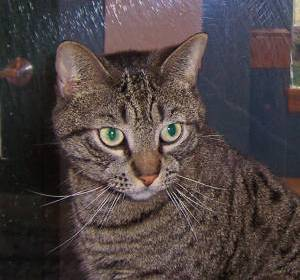
\includegraphics[width=1.2cm]{data/cat.1.jpg}
			};
			\node[anchor=west] (cattext1) at ($ (cat1.east) + (1.2, 0) $) {Katt};
			\draw[->] (cat1) -- (cattext1);
			\node[anchor=north] (dog1) at ($ (cat1.south) + (0, -0.1) $) {
				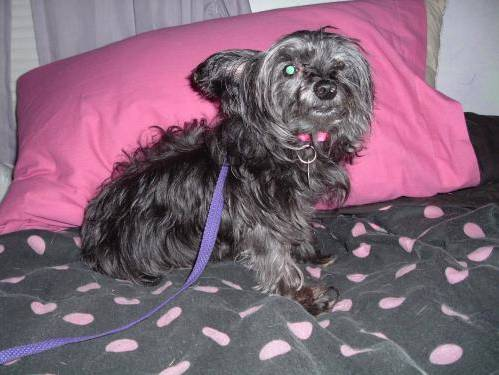
\includegraphics[width=1.2cm]{data/dog.0.jpg}
			};
			\node[anchor=west] (dogtext1) at ($ (dog1.east) + (1.2, 0) $) {Hund};
			\draw[->] (dog1) -- (dogtext1);
			\node[anchor=north] (cat2) at ($ (dog1.south) + (0, -0.1) $) {
				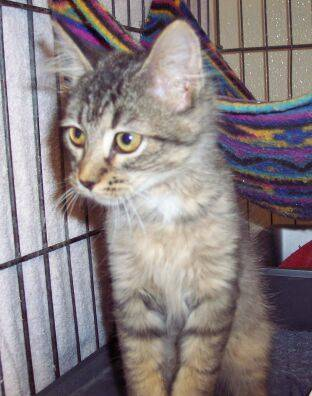
\includegraphics[width=1.2cm]{data/cat.2.jpg}
			};
			\node[anchor=west] (cattext2) at ($ (cat2.east) + (1.2, 0) $) {Katt};
			\draw[->] (cat2) -- (cattext2);
			\node[anchor=north] (dog2) at ($ (cat2.south) + (0, -0.1) $) {
				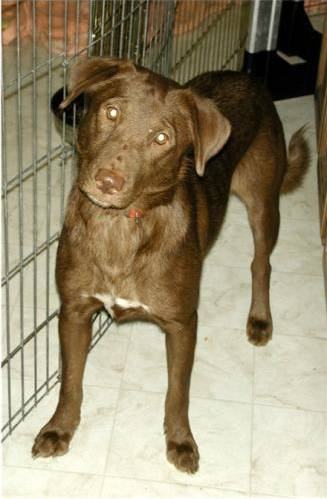
\includegraphics[width=1.2cm]{data/dog.1.jpg}
			};
			\node[anchor=west] (dogtext2) at ($ (dog2.east) + (1.2, 0) $) {Hund};
			\draw[->] (dog2) -- (dogtext2);

			\node[] (cat1) at ($ (unsupervised.south) + (-1.2, -1.1) $) {
				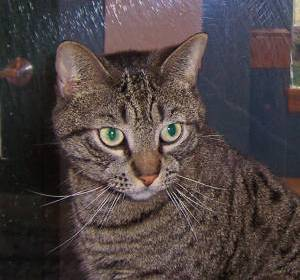
\includegraphics[width=0.8cm]{data/cat.1.jpg}
			};
			\node[] (cat2) at ($ (cat1) + (-0.9, 0.2) $) {
				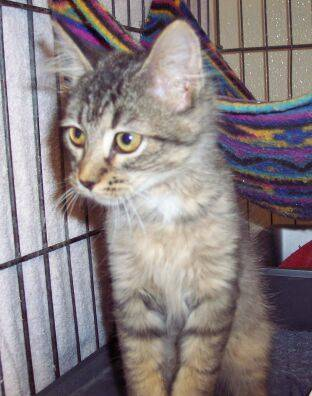
\includegraphics[width=0.8cm]{data/cat.2.jpg}
			};
			\node[] (cat3) at ($ (cat1) + (-0.5, -0.8) $) {
				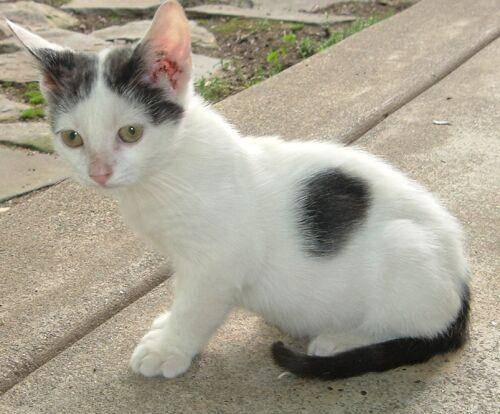
\includegraphics[width=0.8cm]{data/cat.3.jpg}
			};
			\node[] (cat4) at ($ (cat1) + (0.9, -0.1) $) {
				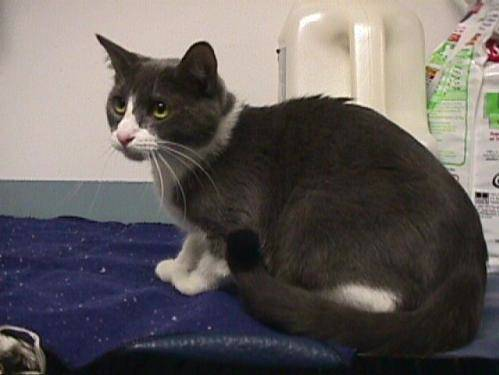
\includegraphics[width=0.8cm]{data/cat.4.jpg}
			};

			\node[] (dog1) at ($ (cat1) + (1.8, -1.5) $) {
				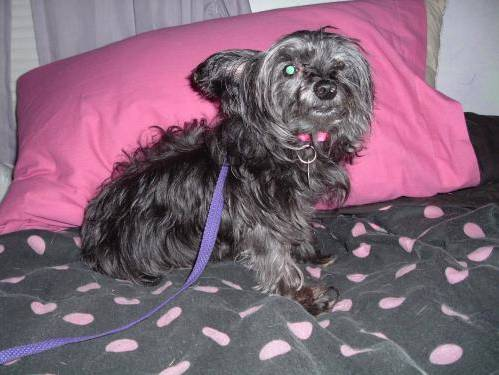
\includegraphics[width=0.8cm]{data/dog.0.jpg}
			};
			\node[] (dog2) at ($ (dog1) + (0.9, 0.1) $) {
				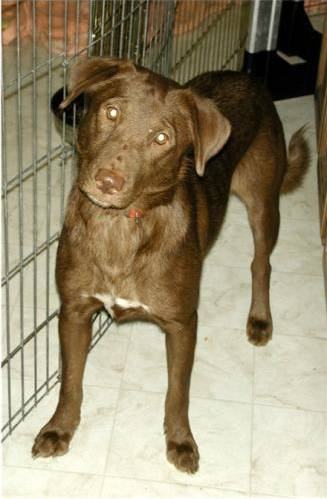
\includegraphics[width=0.8cm]{data/dog.1.jpg}
			};
			\node[] (dog3) at ($ (dog1) + (0.3, -0.8) $) {
				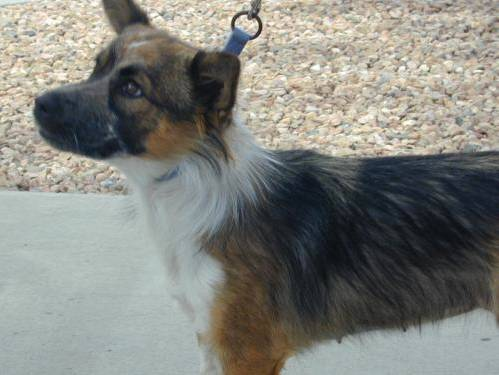
\includegraphics[width=0.8cm]{data/dog.3.jpg}
			};
			\node[] (dog4) at ($ (dog1) + (-0.9, -0.3) $) {
				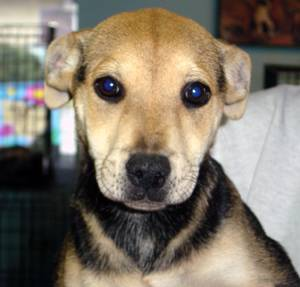
\includegraphics[width=0.8cm]{data/dog.4.jpg}
			};
			\draw[dashed, thick, red] ($ (cat1) + (-0.9, -1.7) $) -- ($ (dog1) + (1.2, 1.7) $);
		\end{tikzpicture}
		\vfill
	\end{frame}

	\section{Maskinlæring}

	\begin{frame}{Maskinlæring: Lineær regresjon} % Table
		\small
		\centering
		\vfill
		\begin{tabular}{|c|c|}
			\hline
			\textbf{BMI}&\textbf{Systolisk blodtrykk}\\
			\hline
			28.99&152.43\\
			26.45&153.27\\
			29.59&158.09\\
			33.09&168.63\\
			26.06&146.40\\
			26.06&136.18\\
			33.32&175.97\\
			30.07&150.52\\
			25.12&131.41\\
			29.17&157.25\\
			25.15&141.85\\
			25.14&138.97\\
			27.97&150.28\\
			19.35&110.56\\
			20.10&108.06\\
			24.75&132.78\\
			22.95&125.97\\
			28.26&157.44\\
			23.37&131.87\\
			21.35&112.26\\
			\hline
		\end{tabular}
		\vfill
	\end{frame}


	\newsavebox{\linearpoints}
	\sbox{\linearpoints}{%
		\begin{tikzpicture}
			\begin{axis}[
				xlabel=BMI,
				ylabel={Systolisk blodtrykk},
				height=6cm,
				width=6cm,
				xmin=18,
				xmax=35.5,
				ymin=102,
				ymax=178,
				xtick pos=bottom,
				ytick pos=left
			]
				\addplot[
					only marks,
					blue!60,
					mark size=2pt,
					opacity=0.5,
				] coordinates {
					(28.99,152.43)
					(26.45,153.27)
					(29.59,158.09)
					(33.09,168.63)
					(26.06,146.40)
					(26.06,136.18)
					(33.32,175.97)
					(30.07,150.52)
					(25.12,131.41)
					(29.17,157.25)
					(25.15,141.85)
					(25.14,138.97)
					(27.97,150.28)
					(19.35,110.56)
					(20.10,108.06)
					(24.75,132.78)
					(22.95,125.97)
					(28.26,157.44)
					(23.37,131.87)
					(21.35,112.26)
					(32.86,174.50)
					(26.10,140.51)
					(27.27,144.33)
					(21.30,123.91)
					(24.82,141.86)
					(27.44,153.15)
					(22.40,121.59)
					(28.50,151.72)
					(24.60,137.34)
					(25.83,146.13)
				};
			\end{axis}
		\end{tikzpicture}
	}

	\begin{frame}{Maskinlæring: Lineær regresjon} % Linear points
		\centering

		\begin{tikzpicture}
			\node[] at (0, 0) {
				\usebox{\linearpoints}
			};
			\node[] at (-4, -5.5) {};
			\node[] at (4.87, 2.75) {};
		\end{tikzpicture}
	\end{frame}

	\newsavebox{\linearbox}
	\sbox{\linearbox}{%
		\begin{tikzpicture}
			\begin{axis}[
				xlabel=BMI,
				ylabel={Systolisk blodtrykk},
				height=6cm,
				width=6cm,
				xmin=18,
				xmax=35.5,
				ymin=102,
				ymax=178,
				xtick pos=bottom,
				ytick pos=left
			]
				\addplot[
					only marks,
					blue!60,
					mark size=2pt,
					opacity=0.5,
				] coordinates {
					(28.99,152.43)
					(26.45,153.27)
					(29.59,158.09)
					(33.09,168.63)
					(26.06,146.40)
					(26.06,136.18)
					(33.32,175.97)
					(30.07,150.52)
					(25.12,131.41)
					(29.17,157.25)
					(25.15,141.85)
					(25.14,138.97)
					(27.97,150.28)
					(19.35,110.56)
					(20.10,108.06)
					(24.75,132.78)
					(22.95,125.97)
					(28.26,157.44)
					(23.37,131.87)
					(21.35,112.26)
					(32.86,174.50)
					(26.10,140.51)
					(27.27,144.33)
					(21.30,123.91)
					(24.82,141.86)
					(27.44,153.15)
					(22.40,121.59)
					(28.50,151.72)
					(24.60,137.34)
					(25.83,146.13)
				};
				\addplot[thick, blue] coordinates {
					(18, 25+4.5*18)
					(35, 25+4.5*35)
				};
			\end{axis}
		\end{tikzpicture}
	}

	\begin{frame}{Maskinlæring: Lineær regresjon} % Linear line
		\centering

		\begin{tikzpicture}
			\node[] at (0, 0) {
				\usebox{\linearbox}
			};
			\node[] at (-4, -5.5) {};
			\node[] at (4.87, 2.75) {};
		\end{tikzpicture}
	\end{frame}

	\begin{frame}{Maskinlæring: Lineær regresjon} % Linear formula
		\centering

		\begin{tikzpicture}
			\node[] at (0, 0) {
				\usebox{\linearbox}
			};
			\node[] at (0.85, -3.5) {
				$SBP=25+4.5*BMI$
			};
			\node[] at (-4, -5.5) {};
			\node[] at (4.87, 2.75) {};
		\end{tikzpicture}
	\end{frame}

	\newsavebox{\linearmodel}
	\sbox{\linearmodel}{%
		\begin{tikzpicture}
			\node[draw=black] (in) at (-1.25, -0.75) {BMI};

			\node[minimum width=3.1cm, minimum height=1.2cm, draw=black, fill=gray!10] at (1.2, -0.75) {$25+4.5*BMI$};
			\node[anchor=south] at (1.2, -0.15) {\small{Lineær modell}};

			\node[draw=black, align=center, dashed] (out) at (4.1, -0.75) {Systolisk\\blodtrykk};

			\draw[->] (in) -- (-0.35, -0.75);
			\draw[->] (2.75, -0.75) -- (out);
		\end{tikzpicture}
	}

	\begin{frame}{Maskinlæring: Lineær regresjon} % Linear model
		\centering

		\begin{tikzpicture}
			\node[] at (0, 0) {
				\usebox{\linearbox}
			};
			\node[] at (0.85, -4) {
				\usebox{\linearmodel}
			};
			\node[] at (-4, -5.5) {};
			\node[] at (4.87, 2.75) {};
		\end{tikzpicture}
	\end{frame}

	\newsavebox{\nonlinearpoints}
	\sbox{\nonlinearpoints}{%
		\begin{tikzpicture}
			\begin{axis}[
				xlabel=BMI,
				ylabel={Systolisk blodtrykk},
				height=6cm,
				width=6cm,
				xmin=18,
				xmax=35.5,
				ymin=102,
				ymax=178,
				xtick pos=bottom,
				ytick pos=left
			]
				\addplot[
					only marks,
					blue!60,
					mark size=2pt,
					opacity=0.5,
				] coordinates {
					(25.20,141.07)
					(27.00,164.47)
					(21.02,111.24)
					(27.77,159.40)
					(23.33,116.16)
					(18.66,112.62)
					(22.41,120.45)
					(27.39,167.73)
					(26.33,156.61)
					(20.41,112.99)
					(27.47,161.91)
					(24.65,136.30)
					(26.70,156.69)
					(26.33,157.41)
					(20.37,110.19)
					(26.40,160.58)
					(22.57,113.96)
					(31.19,173.48)
					(27.89,166.26)
					(25.18,145.27)
					(21.07,113.51)
					(25.22,137.73)
					(25.64,149.39)
					(20.16,110.58)
					(33.89,167.66)
					(26.58,160.27)
					(31.77,165.56)
					(20.55,112.36)
					(31.54,171.44)
					(19.56,111.16)
				};
			\end{axis}
		\end{tikzpicture}
	}

	\begin{frame}{Maskinlæring: Dype nevrale nettverk} % Non-linear points
		\centering

		\begin{tikzpicture}
			\node[] at (0, 0) {
				\usebox{\nonlinearpoints}
			};
			\node[] at (-4, -5.5) {};
			\node[] at (4.87, 2.75) {};
		\end{tikzpicture}
	\end{frame}

	\newsavebox{\nonlinearbox}
	\sbox{\nonlinearbox}{%
		\begin{tikzpicture}
			\begin{axis}[
				xlabel=BMI,
				ylabel={Systolisk blodtrykk},
				height=6cm,
				width=6cm,
				xmin=18,
				xmax=35.5,
				ymin=102,
				ymax=178,
				xtick pos=bottom,
				ytick pos=left
			]
				\addplot[
					only marks,
					blue!60,
					mark size=2pt,
					opacity=0.5,
				] coordinates {
					(25.20,141.07)
					(27.00,164.47)
					(21.02,111.24)
					(27.77,159.40)
					(23.33,116.16)
					(18.66,112.62)
					(22.41,120.45)
					(27.39,167.73)
					(26.33,156.61)
					(20.41,112.99)
					(27.47,161.91)
					(24.65,136.30)
					(26.70,156.69)
					(26.33,157.41)
					(20.37,110.19)
					(26.40,160.58)
					(22.57,113.96)
					(31.19,173.48)
					(27.89,166.26)
					(25.18,145.27)
					(21.07,113.51)
					(25.22,137.73)
					(25.64,149.39)
					(20.16,110.58)
					(33.89,167.66)
					(26.58,160.27)
					(31.77,165.56)
					(20.55,112.36)
					(31.54,171.44)
					(19.56,111.16)
				};
				\addplot[smooth, blue, thick] coordinates {
					(18, 110)
					(23, 117)
					(28, 165)
					(36, 175)
				};
			\end{axis}
		\end{tikzpicture}
	}

	\begin{frame}{Maskinlæring: Dype nevrale nettverk} % Black box neural net
		\centering

		\newsavebox{\blackbox}
		\sbox{\blackbox}{%
			\begin{tikzpicture}
				\node[draw=black] (in) at (-1.25, -0.75) {BMI};

				\node[minimum width=3.1cm, minimum height=2.2cm, draw=black, fill=gray!70] at (1.2, -0.75) {};
				\node[anchor=south] at (1.2, 0.3) {\small{Nevralt nettverk}};

				\node[draw=black, align=center, dashed] (out) at (4.1, -0.75) {Systolisk\\blodtrykk};

				\draw[->] (in) -- (-0.35, -0.75);
				\draw[->] (2.75, -0.75) -- (out);
			\end{tikzpicture}
		}

		\begin{tikzpicture}
			\node[] at (0, 0) {
				\usebox{\nonlinearbox}
			};
			\node[] at (0.85, -4) {
				\usebox{\blackbox}
			};
			\node[] at (-4, -5.5) {};
			\node[] at (4.87, 2.75) {};
		\end{tikzpicture}
	\end{frame}

	\begin{frame}{Maskinlæring: Dype nevrale nettverk} % Detailed neural net
		\centering

		\newcommand{\graphnode}[3]{
			\node[
				circle,
				fill=cyan!40,
				inner sep=0pt,
				outer sep=0pt,
				minimum width=10pt,
				draw=black
			] (####3) at (####1 * 0.6, ####2 * 0.5) {};
		}

		\newsavebox{\graphbox}
		\sbox{\graphbox}{%
			\begin{tikzpicture}
				\node[draw=black] (in) at (-1.25, -0.75) {BMI};

				\node[minimum width=3.1cm, minimum height=2.2cm, draw=black, fill=gray!10] at (1.2, -0.75) {};
				\node[anchor=south] at (1.2, 0.3) {\small{Nevralt nettverk}};

				\graphnode{0}{0}{n00}
				\graphnode{0}{-1}{n01}
				\graphnode{0}{-2}{n02}
				\graphnode{0}{-3}{n03}
				\graphnode{1}{-0.5}{n10}
				\graphnode{1}{-1.5}{n11}
				\graphnode{1}{-2.5}{n12}
				\graphnode{2}{-0.5}{n20}
				\graphnode{2}{-1.5}{n21}
				\graphnode{2}{-2.5}{n22}
				\graphnode{3}{-1}{n30}
				\graphnode{3}{-2}{n31}
				\graphnode{4}{-1}{n40}
				\graphnode{4}{-2}{n41}

				\node[draw=black, align=center, dashed] (out) at (4.1, -0.75) {Systolisk\\blodtrykk};

				\draw[] (n00) -- (n10);
				\draw[] (n00) -- (n11);
				\draw[] (n00) -- (n12);
				\draw[] (n01) -- (n10);
				\draw[] (n01) -- (n11);
				\draw[] (n01) -- (n12);
				\draw[] (n02) -- (n10);
				\draw[] (n02) -- (n11);
				\draw[] (n02) -- (n12);
				\draw[] (n03) -- (n10);
				\draw[] (n03) -- (n11);
				\draw[] (n03) -- (n12);
				\draw[] (n10) -- (n20);
				\draw[] (n10) -- (n21);
				\draw[] (n10) -- (n22);
				\draw[] (n11) -- (n20);
				\draw[] (n11) -- (n21);
				\draw[] (n11) -- (n22);
				\draw[] (n12) -- (n20);
				\draw[] (n12) -- (n21);
				\draw[] (n12) -- (n22);
				\draw[] (n20) -- (n30);
				\draw[] (n20) -- (n31);
				\draw[] (n21) -- (n30);
				\draw[] (n21) -- (n31);
				\draw[] (n22) -- (n30);
				\draw[] (n22) -- (n31);
				\draw[] (n30) -- (n40);
				\draw[] (n30) -- (n41);
				\draw[] (n31) -- (n40);
				\draw[] (n31) -- (n41);

				\draw[] (-0.35, -0.75) -- (n00);
				\draw[] (-0.35, -0.75) -- (n01);
				\draw[] (-0.35, -0.75) -- (n02);
				\draw[] (-0.35, -0.75) -- (n03);

				\draw[] (2.75, -0.75) -- (n40);
				\draw[] (2.75, -0.75) -- (n41);

				\draw[->] (in) -- (-0.35, -0.75);
				\draw[->] (2.75, -0.75) -- (out);
			\end{tikzpicture}
		}

		\begin{tikzpicture}
			\node[] at (0, 0) {
				\usebox{\nonlinearbox}
			};
			\node[] at (0.85, -4) {
				\usebox{\graphbox}
			};
			\node[] at (-4, -5.5) {};
			\node[] at (4.87, 2.75) {};
		\end{tikzpicture}
	\end{frame}

	\begin{frame}{Maskinlæring: Ustrukturert data}
		\newsavebox{\eegbox}
		\sbox{\eegbox}{%
		\begin{tikzpicture}
			\begin{axis}[
				height=3cm,
				width=6cm,
				xmajorticks=false,
				ymajorticks=false,
				axis line style={draw=none}
			]
				\addplot[samples=500,domain=0:1,red,thick] {1.5*sin(deg(2*pi*10*x)) + 0.5*sin(deg(2*pi*7*x))};
			\end{axis}
		\end{tikzpicture}
		}
		\centering
		\vfill
		\begin{tikzpicture}
			{
				\small
				\node[label={Strukturert data}] at (0, -1) {
					\begin{tabular}{|c|c|c|c|}
						\hline
						\textbf{Alder}&\textbf{Kjønn}&\textbf{BMI}&\textbf{SBP}\\
						\hline
						54&M&28.99&152\\
						32&K&26.45&110\\
						41&K&21.59&91\\
						72&M&25.52&130\\
						\hline
					\end{tabular}
				};
			}

			\draw[dashed] (3, 2.5) -- (3, -4.5);

			\node[align=center, anchor=west] at (3.7, 1.5) {
				"Pasienten opplever\\smerter i brystet og\\har høyt blodtrykk."
			};

			\node[draw=black, fill=black, anchor=west] at (3.8, -0.9) {
				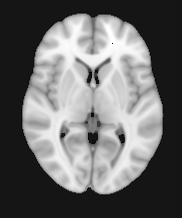
\includegraphics[width=2cm]{data/slice_10.png}
			};

			\node[anchor=west, inner sep=0pt] at (3.5, -3.5) {
				\usebox{\eegbox}
			};

			\node[anchor=west] at (3.7, 2.5) {\underline{\textbf{Ustrukturert data}}};

		\end{tikzpicture}
		\vfill
	\end{frame}

	\begin{frame}{Kunstig intelligens: Oppsummering}
		\centering
		\vfill
		\begin{itemize}
			\item Kunstig intelligens er et fagfelt som handler om å lage maskiner som løser vanskelige oppgaver som tidligere var reservert for mennesker.
			\item Maskinlæring er en teknikk der en maskin lærer å løse et problem gjennom å finne mønster i data.
			\item Nevrale nett er en type maskinlæringsmodell inspirert av hjernen, der prediksjonen skjer via et nettverk av kunstige nevroner.
			\begin{itemize}
				\item[\textcolor{green}{+}] Kan modellere komplekse, ikke-lineære sammenhenger.
				\item[\textcolor{green}{+}] Er i stand til å håndtere ikke-strukturert data (e.g. bilder).
				\item[\textcolor{red}{-}] Reglene som modellen lærer er ikke nødvendigvis forståelig for mennesker.
				\item[\textcolor{red}{-}] Krever mye data og regnekraft.
				\item[\textcolor{red}{-}] Kan være slutten på menneskeheten(?)
			\end{itemize}
		\end{itemize}
		\vfill
	\end{frame}

	\section{Bildegjenkjenning}

	\begin{frame}{Bildegjenkjenning} % Images
		\vfill
		\centering
		\begin{tikzpicture}
			\node[label=below:Katt] at (-5, 0) {
				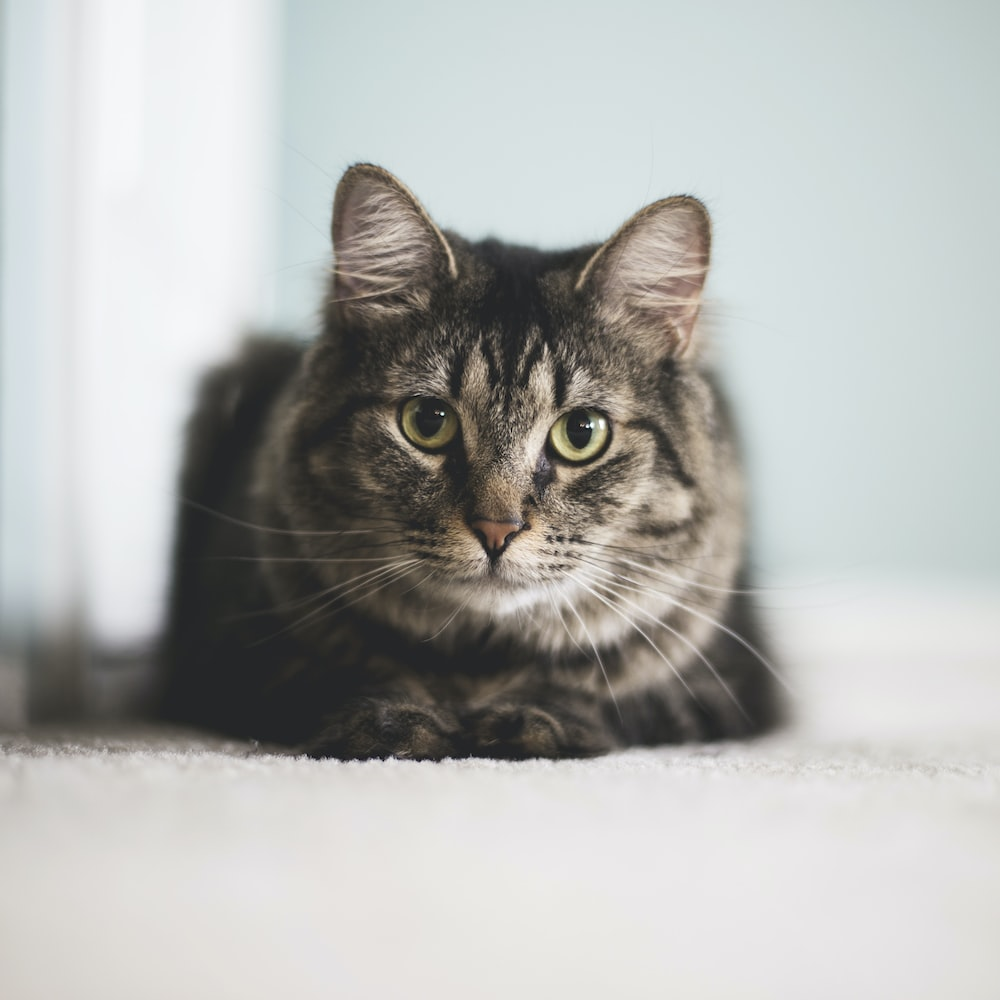
\includegraphics[width=2cm]{data/cat.jpeg}
			};
			\node[label=below:Solsikke] at (-2.5, 0) {
				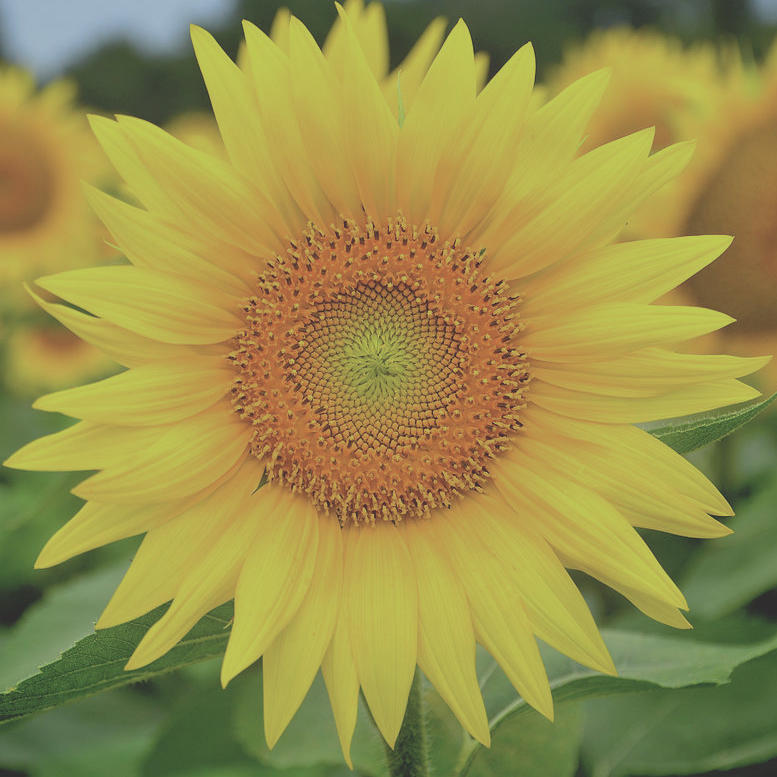
\includegraphics[width=2cm]{data/sunflower.jpeg}
			};
			\node[label=below:Hvithai] at (0, 0) {
				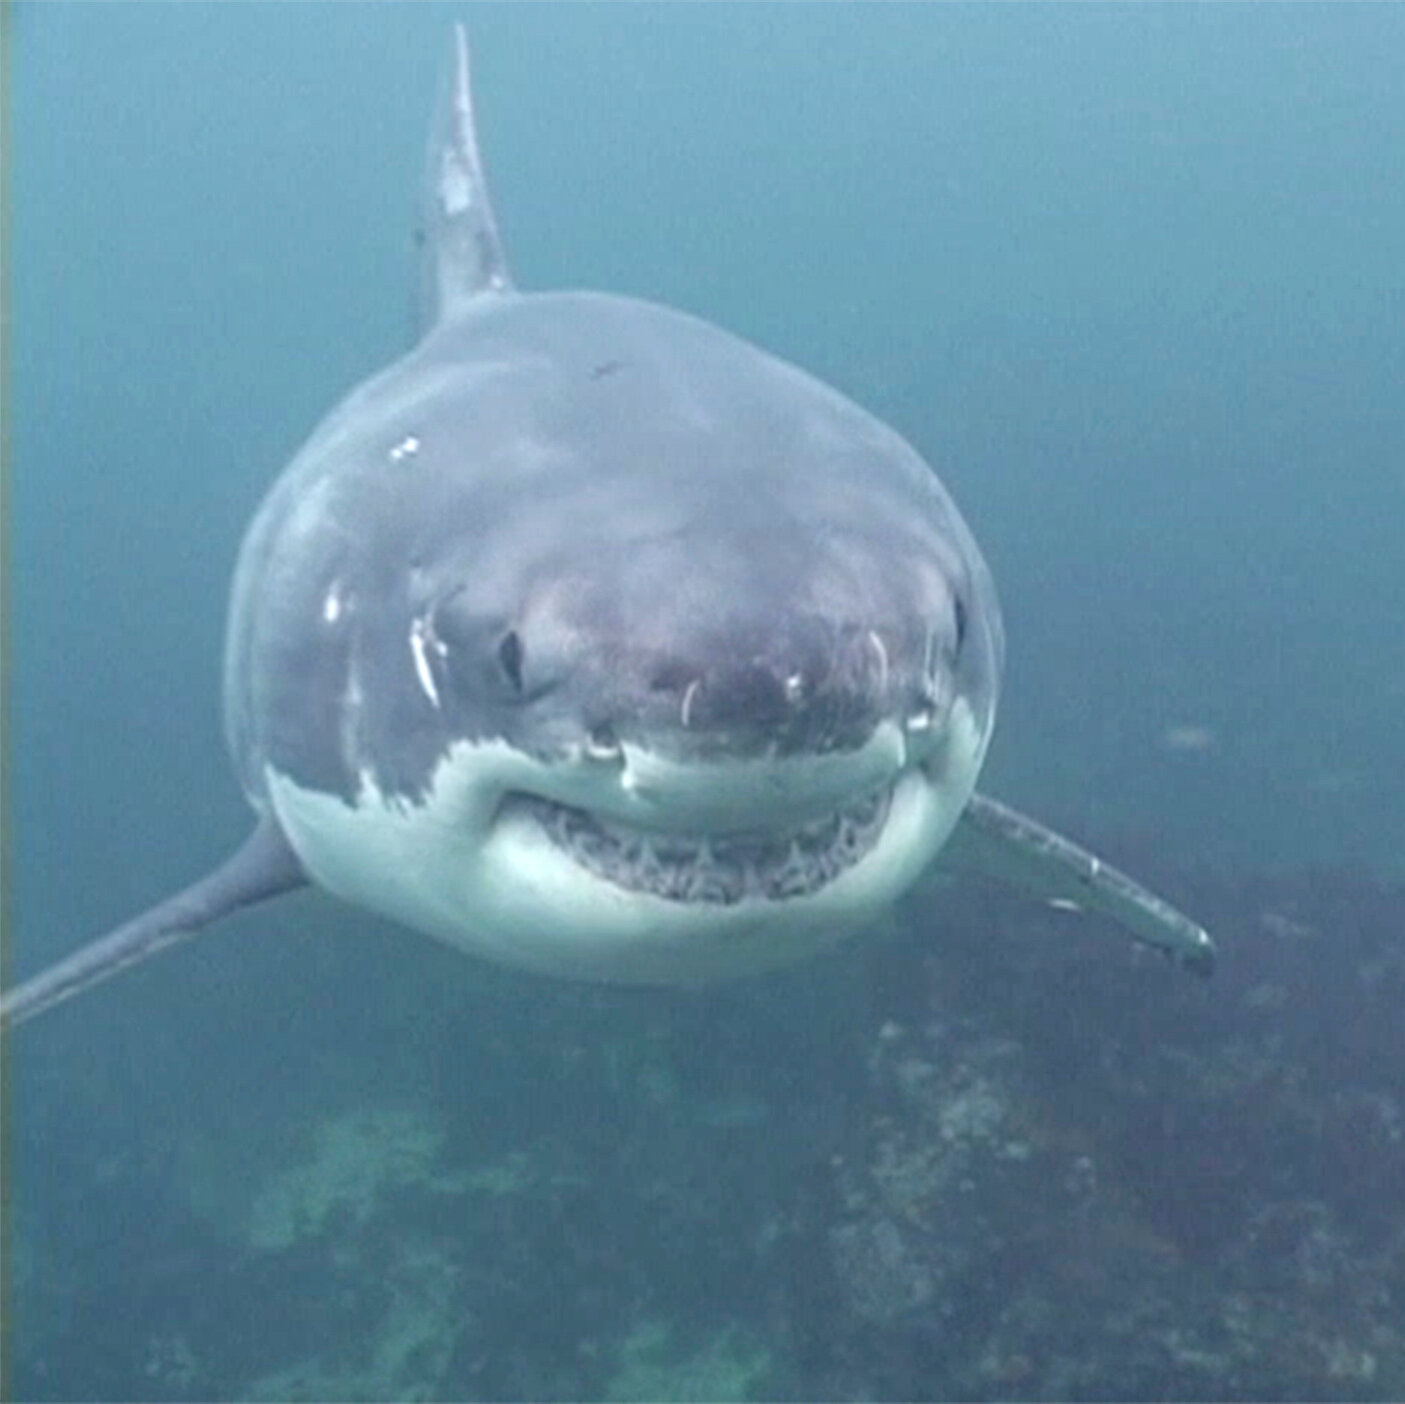
\includegraphics[width=2cm]{data/shark.jpeg}
			};
			\node[label=below:Fly] at (2.5, 0) {
				
\includegraphics[width=2cm]{data/airplane.jpeg}
			};
			\node[] at (-1.25, -3) {};
		\end{tikzpicture}
		\centering
	\end{frame}

	\begin{frame}{Bildegjenkjenning} % Imagenet
		\vfill
		\centering
		\begin{tikzpicture}
			\node[label=below:Katt] at (-5, 0) {
				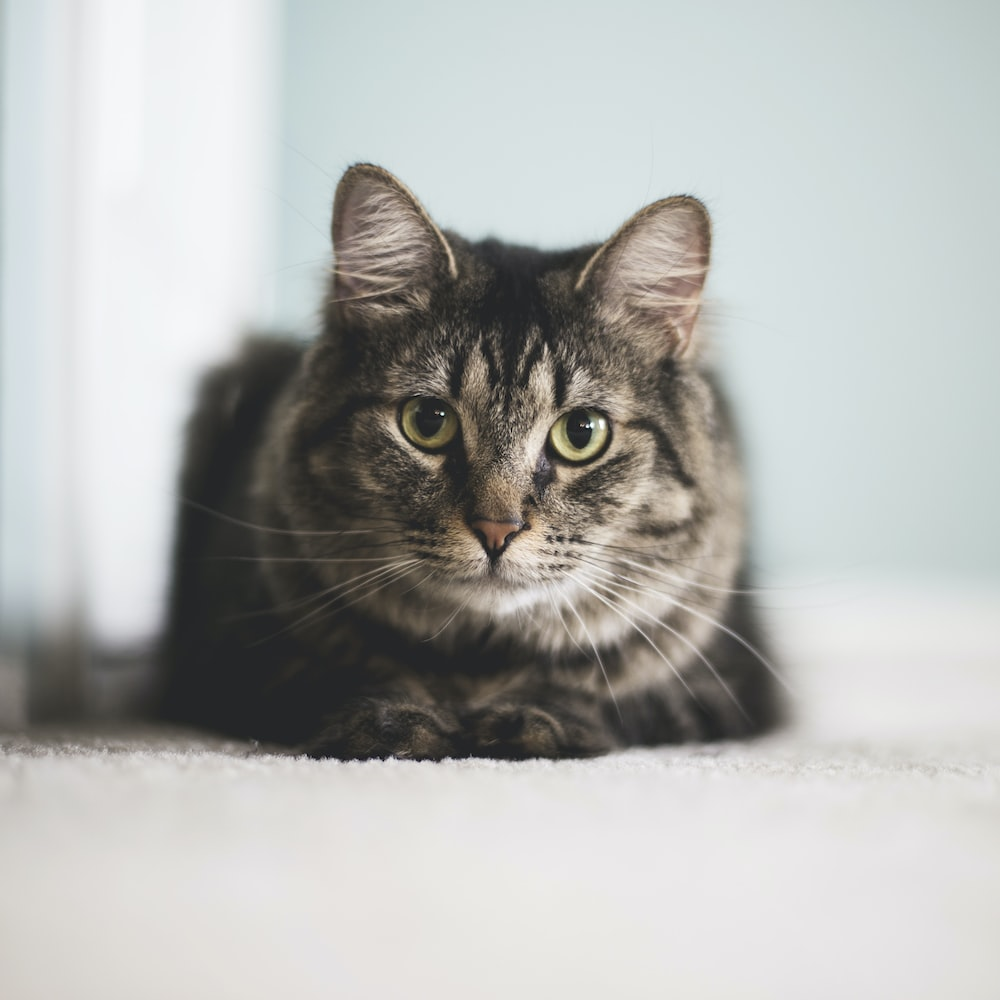
\includegraphics[width=2cm]{data/cat.jpeg}
			};
			\node[label=below:Solsikke] at (-2.5, 0) {
				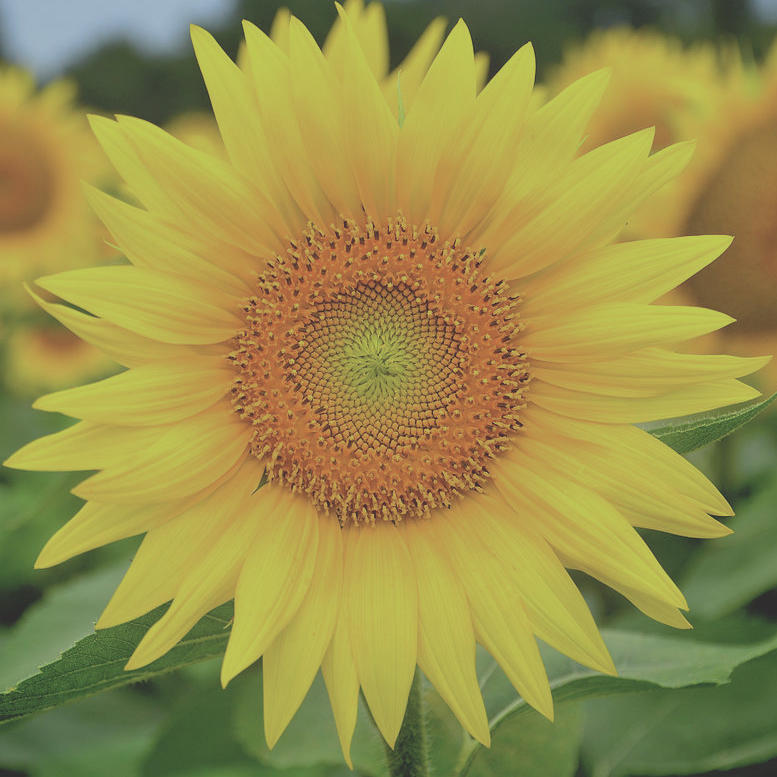
\includegraphics[width=2cm]{data/sunflower.jpeg}
			};
			\node[label=below:Hvithai] at (0, 0) {
				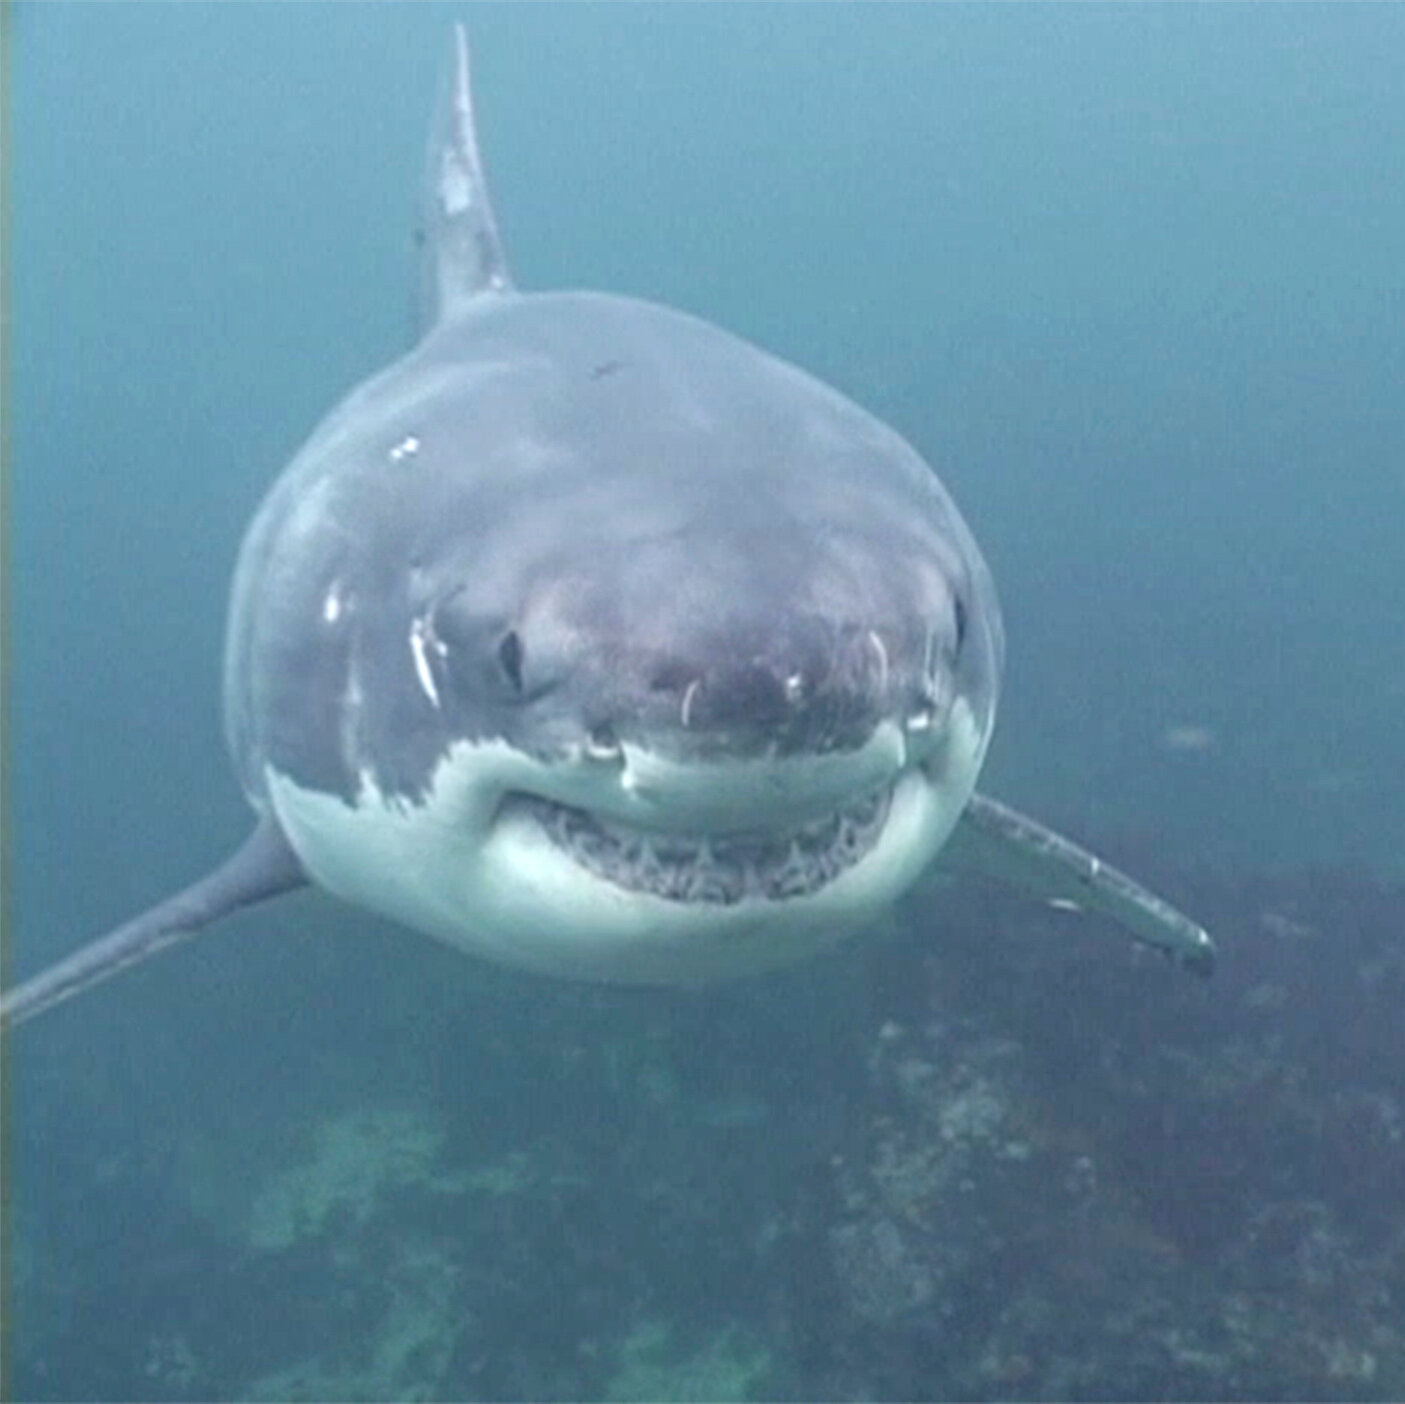
\includegraphics[width=2cm]{data/shark.jpeg}
			};
			\node[label=below:Fly] at (2.5, 0) {
				
\includegraphics[width=2cm]{data/airplane.jpeg}
			};

			\node[] at (-1.25, -2) {
				ImageNet: $\sim$14 millioner bilder, 1000 kategorier
			};

			\node[] at (-1.25, -3) {};
		\end{tikzpicture}
		\centering
	\end{frame}

	\begin{frame}{Bildegjenkjenning: Historikk} % Imagenet 2010
		\centering
		\vfill
		\begin{tikzpicture}
			\begin{axis}[
				ylabel={Feilrate},
				xlabel={År},
				xtick={2010, 2012, 2014, 2016, 2018, 2020},
				xticklabels={2010, 2012, 2014, 2016, 2018, 2020},
				ytick={0, 10, 20, 30},
				yticklabels={0\%, 10\%, 20\%, 30\%},
				ytick style={draw=none},
				ytick pos=left,
				xtick pos=bottom,
				ymajorgrids=true,
				ymax=29,
				ymin=0,
				xmin=2009,
				xmax=2021
			]
				\addplot[mark=*, purple,thick] coordinates {
					(2010, 28.2)
				};

				\node[anchor=north, inner sep=5pt] at (axis cs: 2010, 28.2) {
					\textbf{28.2}
				};
			\end{axis}
		\end{tikzpicture}
		\vfill
	\end{frame}

	\begin{frame}{Bildegjenkjenning: Historikk} % Imagenet 2011
		\centering
		\vfill
		\begin{tikzpicture}
			\begin{axis}[
				ylabel={Feilrate},
				xlabel={År},
				xtick={2010, 2012, 2014, 2016, 2018, 2020},
				xticklabels={2010, 2012, 2014, 2016, 2018, 2020},
				ytick={0, 10, 20, 30},
				yticklabels={0\%, 10\%, 20\%, 30\%},
				ytick style={draw=none},
				ytick pos=left,
				xtick pos=bottom,
				ymajorgrids=true,
				ymax=29,
				ymin=0,
				xmin=2009,
				xmax=2021
			]
				\addplot[mark=*, purple,thick] coordinates {
					(2010, 28.2)
					(2011, 25.8)
				};

				\node[anchor=north, inner sep=5pt] at (axis cs: 2010, 28.2) {
					28.2
				};

				\node[anchor=north, inner sep=5pt] at (axis cs: 2011, 25.8) {
					\textbf{25.8}
				};
			\end{axis}
		\end{tikzpicture}
		\vfill
	\end{frame}

	\begin{frame}{Bildegjenkjenning: Historikk} % Imagenet CNNs
		\centering
		\vfill
		\begin{tikzpicture}
			\begin{axis}[
				ylabel={Feilrate},
				xlabel={År},
				xtick={2010, 2012, 2014, 2016, 2018, 2020},
				xticklabels={2010, 2012, 2014, 2016, 2018, 2020},
				ytick={0, 10, 20, 30},
				yticklabels={0\%, 10\%, 20\%, 30\%},
				ytick style={draw=none},
				ytick pos=left,
				xtick pos=bottom,
				ymajorgrids=true,
				ymax=29,
				ymin=0,
				xmin=2009,
				xmax=2021
			]
				\addplot[mark=*, purple,thick] coordinates {
					(2010, 28.2)
					(2011, 25.8)
				};

				\node[anchor=north, inner sep=5pt] at (axis cs: 2010, 28.2) {
					28.2
				};

				\node[anchor=north, inner sep=5pt] at (axis cs: 2011, 25.8) {
					\textbf{25.8}
				};

				\addplot[densely dotted] coordinates {
					(2011.5, 30)
					(2011.5, 0)
				};

				\node[anchor=north west] at (axis cs: 2011.5, 29) {
					CNN
				};
			\end{axis}
		\end{tikzpicture}
		\vfill
	\end{frame}

	\begin{frame}{Bildegjenkjenning: Historikk} % Imagenet 2012
		\centering
		\vfill
		\begin{tikzpicture}
			\begin{axis}[
				ylabel={Feilrate},
				xlabel={År},
				xtick={2010, 2012, 2014, 2016, 2018, 2020},
				xticklabels={2010, 2012, 2014, 2016, 2018, 2020},
				ytick={0, 10, 20, 30},
				yticklabels={0\%, 10\%, 20\%, 30\%},
				ytick style={draw=none},
				ytick pos=left,
				xtick pos=bottom,
				ymajorgrids=true,
				ymax=29,
				ymin=0,
				xmin=2009,
				xmax=2021
			]
				\addplot[mark=*, purple,thick] coordinates {
					(2010, 28.2)
					(2011, 25.8)
					(2012, 16.4)
				};

				\addplot[densely dotted] coordinates {
					(2011.5, 30)
					(2011.5, 0)
				};

				\node[anchor=north, inner sep=5pt] at (axis cs: 2010, 28.2) {
					28.2
				};
				\node[anchor=north, inner sep=5pt] at (axis cs: 2011, 25.8) {
					25.8
				};
				\node[anchor=north, inner sep=5pt] at (axis cs: 2012, 16.4) {
					\textbf{16.4}
				};

				\node[anchor=north west] at (axis cs: 2011.5, 29) {
					CNN
				};
			\end{axis}
		\end{tikzpicture}
		\vfill
	\end{frame}

	\begin{frame}{Bildegjenkjenning: Historikk} % Imagenet 2020
		\centering
		\vfill
		\begin{tikzpicture}
			\begin{axis}[
				ylabel={Feilrate},
				xlabel={År},
				xtick={2010, 2012, 2014, 2016, 2018, 2020},
				xticklabels={2010, 2012, 2014, 2016, 2018, 2020},
				ytick={0, 10, 20, 30},
				yticklabels={0\%, 10\%, 20\%, 30\%},
				ytick style={draw=none},
				ytick pos=left,
				xtick pos=bottom,
				ymajorgrids=true,
				ymax=29,
				ymin=0,
				xmin=2009,
				xmax=2021
			]
				\addplot[mark=*, purple,thick] coordinates {
					(2010, 28.2)
					(2011, 25.8)
					(2012, 16.4)
					(2013, 11.7)
					(2014, 7.3)
					(2015, 3.5)
					(2016, 3.0)
					(2017, 2.3)
					(2018, 1.8)
					(2019, 1.3)
					(2020, 0.9)
				};

				\addplot[densely dotted] coordinates {
					(2011.5, 30)
					(2011.5, 0)
				};

				\node[anchor=north, inner sep=5pt] at (axis cs: 2010, 28.2) {
					28.2
				};
				\node[anchor=north, inner sep=5pt] at (axis cs: 2011, 25.8) {
					25.8
				};
				\node[anchor=north, inner sep=5pt] at (axis cs: 2012, 16.4) {
					16.4
				};
				\node[anchor=north, inner sep=5pt] at (axis cs: 2013, 11.7) {
					11.7
				};
				\node[anchor=north, inner sep=5pt] at (axis cs: 2014, 7.3) {
					7.3
				};
				\node[anchor=north, inner sep=5pt] at (axis cs: 2015, 3.5) {
					3.5
				};
				\node[anchor=north, inner sep=5pt] at (axis cs: 2016, 3.0) {
					3.0
				};
				\node[anchor=south, inner sep=5pt] at (axis cs: 2017, 2.3) {
					2.3
				};
				\node[anchor=south, inner sep=5pt] at (axis cs: 2018, 1.8) {
					1.8
				};
				\node[anchor=south, inner sep=5pt] at (axis cs: 2019, 1.3) {
					1.3
				};
				\node[anchor=south, inner sep=5pt] at (axis cs: 2020, 0.9) {
					\textbf{0.9}
				};

				\node[anchor=north west] at (axis cs: 2011.5, 29) {
					CNN
				};
			\end{axis}
		\end{tikzpicture}
		\vfill
	\end{frame}

	\begin{frame}{Bildegjenkjenning: Historikk} % Imagenet human
		\centering
		\vfill
		\begin{tikzpicture}
			\begin{axis}[
				ylabel={Feilrate},
				xlabel={År},
				xtick={2010, 2012, 2014, 2016, 2018, 2020},
				xticklabels={2010, 2012, 2014, 2016, 2018, 2020},
				ytick={0, 10, 20, 30},
				yticklabels={0\%, 10\%, 20\%, 30\%},
				ytick style={draw=none},
				ytick pos=left,
				xtick pos=bottom,
				ymajorgrids=true,
				ymax=29,
				ymin=0,
				xmin=2009,
				xmax=2021
			]
				\addplot[mark=*, purple,thick] coordinates {
					(2010, 28.2)
					(2011, 25.8)
					(2012, 16.4)
					(2013, 11.7)
					(2014, 7.3)
					(2015, 3.5)
					(2016, 3.0)
					(2017, 2.3)
					(2018, 1.8)
					(2019, 1.3)
					(2020, 0.9)
				};

				\node[anchor=north, inner sep=5pt] at (axis cs: 2010, 28.2) {
					28.2
				};
				\node[anchor=north, inner sep=5pt] at (axis cs: 2011, 25.8) {
					25.8
				};
				\node[anchor=north, inner sep=5pt] at (axis cs: 2012, 16.4) {
					16.4
				};
				\node[anchor=north, inner sep=5pt] at (axis cs: 2013, 11.7) {
					11.7
				};
				\node[anchor=north, inner sep=5pt] at (axis cs: 2014, 7.3) {
					7.3
				};
				\node[anchor=north, inner sep=5pt] at (axis cs: 2015, 3.5) {
					3.5
				};
				\node[anchor=north, inner sep=5pt] at (axis cs: 2016, 3.0) {
					3.0
				};
				\node[anchor=south, inner sep=5pt] at (axis cs: 2017, 2.3) {
					2.3
				};
				\node[anchor=south, inner sep=5pt] at (axis cs: 2018, 1.8) {
					1.8
				};
				\node[anchor=south, inner sep=5pt] at (axis cs: 2019, 1.3) {
					1.3
				};
				\node[anchor=south, inner sep=5pt] at (axis cs: 2020, 0.9) {
					\textbf{0.9}
				};

				\addplot[densely dotted] coordinates {
					(2011.5, 30)
					(2011.5, 0)
				};

				\addplot[dashed, red] coordinates {
					(2009, 5.1)
					(2021, 5.1)
				};

				\node[anchor=north west] at (axis cs: 2011.5, 29) {
					CNN
				};

				\node[anchor=south east] at (axis cs: 2021, 5.1) {
					\textcolor{red}{Menneskelig nivå}
				};
			\end{axis}
		\end{tikzpicture}
		\vfill
	\end{frame}

	\begin{frame}{Bildegjenkjenning: Konvolusjonelle nevrale nettverk} % Flower
		\centering
		\vfill
		\resizebox{\textwidth}{!}{

		\colorlet{nodefill}{cyan!40}
		\begin{tikzpicture}[
			ampersand replacement=\&
		]
			\node[inner sep=0pt, draw=black] (l0) at (0, 0) {
				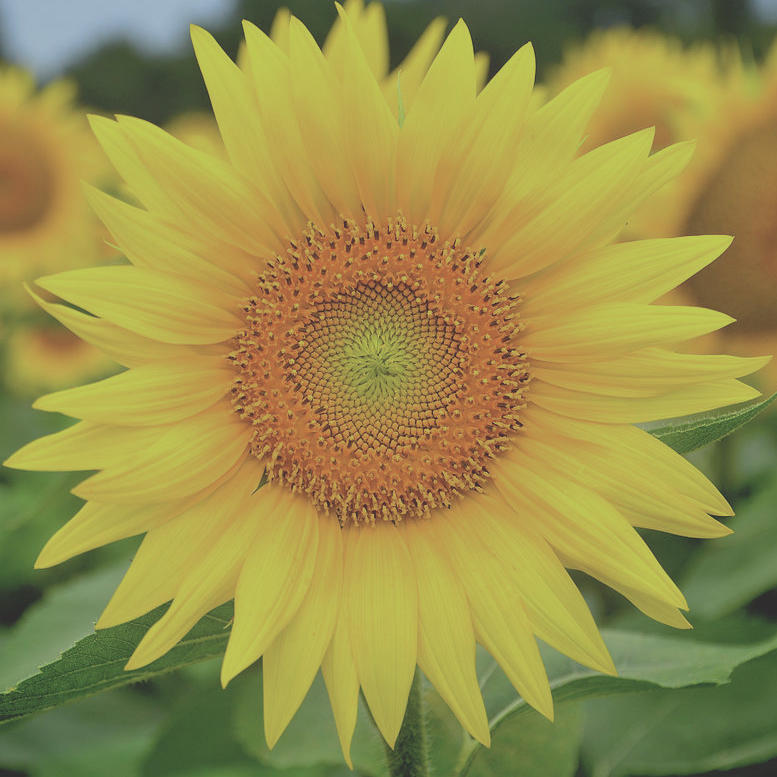
\includegraphics[width=1cm]{data/sunflower.jpeg}
			};

			\matrix[every node/.style={minimum height=0.15cm, minimum width=0.15cm, draw=black, fill=nodefill, inner sep=0pt}] at (1.65, 0.1) {
				\node{}; \& \node{}; \& \node{}; \& \node{}; \& \node{}; \& \node{}; \& \node{}; \& \node{};\\
				\node{}; \& \node{}; \& \node{}; \& \node{}; \& \node{}; \& \node{}; \& \node{}; \& \node{};\\
				\node{}; \& \node{}; \& \node{}; \& \node{}; \& \node{}; \& \node{}; \& \node{}; \& \node{};\\
				\node{}; \& \node{}; \& \node{}; \& \node{}; \& \node{}; \& \node{}; \& \node{}; \& \node{};\\
				\node{}; \& \node{}; \& \node{}; \& \node{}; \& \node{}; \& \node{}; \& \node{}; \& \node{};\\
				\node{}; \& \node{}; \& \node{}; \& \node{}; \& \node{}; \& \node{}; \& \node{}; \& \node{};\\
				\node{}; \& \node{}; \& \node{}; \& \node{}; \& \node{}; \& \node{}; \& \node{}; \& \node{};\\
				\node{}; \& \node{}; \& \node{}; \& \node{}; \& \node{}; \& \node{}; \& \node{}; \& \node{};\\
			};

			\matrix[every node/.style={minimum height=0.15cm, minimum width=0.15cm, draw=black, fill=nodefill, inner sep=0pt, outer sep=0pt}] (l1) at (1.75, 0) {
				\node{}; \& \node{}; \& \node{}; \& \node{}; \& \node{}; \& \node{}; \& \node{}; \& \node{};\\
				\node{}; \& \node{}; \& \node{}; \& \node{}; \& \node{}; \& \node{}; \& \node{}; \& \node{};\\
				\node{}; \& \node{}; \& \node{}; \& \node{}; \& \node{}; \& \node{}; \& \node{}; \& \node{};\\
				\node{}; \& \node{}; \& \node{}; \& \node{}; \& \node{}; \& \node{}; \& \node{}; \& \node{};\\
				\node{}; \& \node{}; \& \node{}; \& \node{}; \& \node{}; \& \node{}; \& \node{}; \& \node{};\\
				\node{}; \& \node{}; \& \node{}; \& \node{}; \& \node{}; \& \node{}; \& \node{}; \& \node{};\\
				\node{}; \& \node{}; \& \node{}; \& \node{}; \& \node{}; \& \node{}; \& \node{}; \& \node{};\\
				\node{}; \& \node{}; \& \node{}; \& \node{}; \& \node{}; \& \node{}; \& \node{}; \& \node{};\\
			};
			\draw[->] (l0) -- (l1);


			\matrix[every node/.style={minimum height=0.15cm, minimum width=0.15cm, draw=black, fill=nodefill, inner sep=0pt}] at (1.85, -0.1) {
				\node{}; \& \node{}; \& \node{}; \& \node{}; \& \node{}; \& \node{}; \& \node{}; \& \node{};\\
				\node{}; \& \node{}; \& \node{}; \& \node{}; \& \node{}; \& \node{}; \& \node{}; \& \node{};\\
				\node{}; \& \node{}; \& \node{}; \& \node{}; \& \node{}; \& \node{}; \& \node{}; \& \node{};\\
				\node{}; \& \node{}; \& \node{}; \& \node{}; \& \node{}; \& \node{}; \& \node{}; \& \node{};\\
				\node{}; \& \node{}; \& \node{}; \& \node{}; \& \node{}; \& \node{}; \& \node{}; \& \node{};\\
				\node{}; \& \node{}; \& \node{}; \& \node{}; \& \node{}; \& \node{}; \& \node{}; \& \node{};\\
				\node{}; \& \node{}; \& \node{}; \& \node{}; \& \node{}; \& \node{}; \& \node{}; \& \node{};\\
				\node{}; \& \node{}; \& \node{}; \& \node{}; \& \node{}; \& \node{}; \& \node{}; \& \node{};\\
			};

			\matrix[every node/.style={minimum height=0.15cm, minimum width=0.15cm, draw=black, fill=nodefill, inner sep=0pt}] at (3.4, 0.1) {
				\node{}; \& \node{}; \& \node{}; \& \node{}; \& \node{}; \& \node{};\\
				\node{}; \& \node{}; \& \node{}; \& \node{}; \& \node{}; \& \node{};\\
				\node{}; \& \node{}; \& \node{}; \& \node{}; \& \node{}; \& \node{};\\
				\node{}; \& \node{}; \& \node{}; \& \node{}; \& \node{}; \& \node{};\\
				\node{}; \& \node{}; \& \node{}; \& \node{}; \& \node{}; \& \node{};\\
				\node{}; \& \node{}; \& \node{}; \& \node{}; \& \node{}; \& \node{};\\
			};

			\matrix[every node/.style={minimum height=0.15cm, minimum width=0.15cm, draw=black, fill=nodefill, inner sep=0pt}] (l2)at (3.5, 0) {
				\node{}; \& \node{}; \& \node{}; \& \node{}; \& \node{}; \& \node{};\\
				\node{}; \& \node{}; \& \node{}; \& \node{}; \& \node{}; \& \node{};\\
				\node{}; \& \node{}; \& \node{}; \& \node{}; \& \node{}; \& \node{};\\
				\node{}; \& \node{}; \& \node{}; \& \node{}; \& \node{}; \& \node{};\\
				\node{}; \& \node{}; \& \node{}; \& \node{}; \& \node{}; \& \node{};\\
				\node{}; \& \node{}; \& \node{}; \& \node{}; \& \node{}; \& \node{};\\
			};
			\draw[->] (l1) -- (l2);


			\matrix[every node/.style={minimum height=0.15cm, minimum width=0.15cm, draw=black, fill=nodefill, inner sep=0pt}] at (3.6, -0.1) {
				\node{}; \& \node{}; \& \node{}; \& \node{}; \& \node{}; \& \node{};\\
				\node{}; \& \node{}; \& \node{}; \& \node{}; \& \node{}; \& \node{};\\
				\node{}; \& \node{}; \& \node{}; \& \node{}; \& \node{}; \& \node{};\\
				\node{}; \& \node{}; \& \node{}; \& \node{}; \& \node{}; \& \node{};\\
				\node{}; \& \node{}; \& \node{}; \& \node{}; \& \node{}; \& \node{};\\
				\node{}; \& \node{}; \& \node{}; \& \node{}; \& \node{}; \& \node{};\\
			};

			\matrix[every node/.style={minimum height=0.15cm, minimum width=0.15cm, draw=black, fill=nodefill, inner sep=0pt}] at (5.05, 0.2) {
				\node{}; \& \node{}; \& \node{}; \& \node{}; \& \node{}; \& \node{};\\
				\node{}; \& \node{}; \& \node{}; \& \node{}; \& \node{}; \& \node{};\\
				\node{}; \& \node{}; \& \node{}; \& \node{}; \& \node{}; \& \node{};\\
				\node{}; \& \node{}; \& \node{}; \& \node{}; \& \node{}; \& \node{};\\
				\node{}; \& \node{}; \& \node{}; \& \node{}; \& \node{}; \& \node{};\\
				\node{}; \& \node{}; \& \node{}; \& \node{}; \& \node{}; \& \node{};\\
			};

			\matrix[every node/.style={minimum height=0.15cm, minimum width=0.15cm, draw=black, fill=nodefill, inner sep=0pt}] at (5.15, 0.1) {
				\node{}; \& \node{}; \& \node{}; \& \node{}; \& \node{}; \& \node{};\\
				\node{}; \& \node{}; \& \node{}; \& \node{}; \& \node{}; \& \node{};\\
				\node{}; \& \node{}; \& \node{}; \& \node{}; \& \node{}; \& \node{};\\
				\node{}; \& \node{}; \& \node{}; \& \node{}; \& \node{}; \& \node{};\\
				\node{}; \& \node{}; \& \node{}; \& \node{}; \& \node{}; \& \node{};\\
				\node{}; \& \node{}; \& \node{}; \& \node{}; \& \node{}; \& \node{};\\
			};

			\matrix[every node/.style={minimum height=0.15cm, minimum width=0.15cm, draw=black, fill=nodefill, inner sep=0pt}] (l3) at (5.25, 0) {
				\node{}; \& \node{}; \& \node{}; \& \node{}; \& \node{}; \& \node{};\\
				\node{}; \& \node{}; \& \node{}; \& \node{}; \& \node{}; \& \node{};\\
				\node{}; \& \node{}; \& \node{}; \& \node{}; \& \node{}; \& \node{};\\
				\node{}; \& \node{}; \& \node{}; \& \node{}; \& \node{}; \& \node{};\\
				\node{}; \& \node{}; \& \node{}; \& \node{}; \& \node{}; \& \node{};\\
				\node{}; \& \node{}; \& \node{}; \& \node{}; \& \node{}; \& \node{};\\
			};
			\draw[->] (l2) -- ($ (l3.west) - (0.1, 0) $);


			\matrix[every node/.style={minimum height=0.15cm, minimum width=0.15cm, draw=black, fill=nodefill, inner sep=0pt}] at (5.35, -0.1) {
				\node{}; \& \node{}; \& \node{}; \& \node{}; \& \node{}; \& \node{};\\
				\node{}; \& \node{}; \& \node{}; \& \node{}; \& \node{}; \& \node{};\\
				\node{}; \& \node{}; \& \node{}; \& \node{}; \& \node{}; \& \node{};\\
				\node{}; \& \node{}; \& \node{}; \& \node{}; \& \node{}; \& \node{};\\
				\node{}; \& \node{}; \& \node{}; \& \node{}; \& \node{}; \& \node{};\\
				\node{}; \& \node{}; \& \node{}; \& \node{}; \& \node{}; \& \node{};\\
			};

			\matrix[every node/.style={minimum height=0.15cm, minimum width=0.15cm, draw=black, fill=nodefill, inner sep=0pt}] at (5.45, -0.2) {
				\node{}; \& \node{}; \& \node{}; \& \node{}; \& \node{}; \& \node{};\\
				\node{}; \& \node{}; \& \node{}; \& \node{}; \& \node{}; \& \node{};\\
				\node{}; \& \node{}; \& \node{}; \& \node{}; \& \node{}; \& \node{};\\
				\node{}; \& \node{}; \& \node{}; \& \node{}; \& \node{}; \& \node{};\\
				\node{}; \& \node{}; \& \node{}; \& \node{}; \& \node{}; \& \node{};\\
				\node{}; \& \node{}; \& \node{}; \& \node{}; \& \node{}; \& \node{};\\
			};

			\matrix[every node/.style={minimum height=0.15cm, minimum width=0.15cm, draw=black, fill=nodefill, inner sep=0pt}] at (6.8, 0.2) {
				\node{}; \& \node{}; \& \node{}; \& \node{};\\
				\node{}; \& \node{}; \& \node{}; \& \node{};\\
				\node{}; \& \node{}; \& \node{}; \& \node{};\\
				\node{}; \& \node{}; \& \node{}; \& \node{};\\
			};

			\matrix[every node/.style={minimum height=0.15cm, minimum width=0.15cm, draw=black, fill=nodefill, inner sep=0pt}] at (6.9, 0.1) {
				\node{}; \& \node{}; \& \node{}; \& \node{};\\
				\node{}; \& \node{}; \& \node{}; \& \node{};\\
				\node{}; \& \node{}; \& \node{}; \& \node{};\\
				\node{}; \& \node{}; \& \node{}; \& \node{};\\
			};

			\matrix[every node/.style={minimum height=0.15cm, minimum width=0.15cm, draw=black, fill=nodefill, inner sep=0pt}] (l4) at (7, 0) {
				\node{}; \& \node{}; \& \node{}; \& \node{};\\
				\node{}; \& \node{}; \& \node{}; \& \node{};\\
				\node{}; \& \node{}; \& \node{}; \& \node{};\\
				\node{}; \& \node{}; \& \node{}; \& \node{};\\
			};
			\draw[->] ($ (l3.east) + (0.1, 0) $) -- ($ (l4.west) + (-0.1, 0) $);


			\matrix[every node/.style={minimum height=0.15cm, minimum width=0.15cm, draw=black, fill=nodefill, inner sep=0pt}] at (7.1, -0.1) {
				\node{}; \& \node{}; \& \node{}; \& \node{};\\
				\node{}; \& \node{}; \& \node{}; \& \node{};\\
				\node{}; \& \node{}; \& \node{}; \& \node{};\\
				\node{}; \& \node{}; \& \node{}; \& \node{};\\
			};
			\matrix[every node/.style={minimum height=0.15cm, minimum width=0.15cm, draw=black, fill=nodefill, inner sep=0pt}] at (7.2, -0.2) {
				\node{}; \& \node{}; \& \node{}; \& \node{};\\
				\node{}; \& \node{}; \& \node{}; \& \node{};\\
				\node{}; \& \node{}; \& \node{}; \& \node{};\\
				\node{}; \& \node{}; \& \node{}; \& \node{};\\
			};

			\matrix[every node/.style={minimum height=0.15cm, minimum width=0.15cm, draw=black, fill=nodefill, inner sep=0pt}] at (8.25, 0.3) {
				\node{}; \& \node{}; \& \node{}; \& \node{};\\
				\node{}; \& \node{}; \& \node{}; \& \node{};\\
				\node{}; \& \node{}; \& \node{}; \& \node{};\\
				\node{}; \& \node{}; \& \node{}; \& \node{};\\
			};

			\matrix[every node/.style={minimum height=0.15cm, minimum width=0.15cm, draw=black, fill=nodefill, inner sep=0pt}] at (8.35, 0.2) {
				\node{}; \& \node{}; \& \node{}; \& \node{};\\
				\node{}; \& \node{}; \& \node{}; \& \node{};\\
				\node{}; \& \node{}; \& \node{}; \& \node{};\\
				\node{}; \& \node{}; \& \node{}; \& \node{};\\
			};

			\matrix[every node/.style={minimum height=0.15cm, minimum width=0.15cm, draw=black, fill=nodefill, inner sep=0pt}] at (8.45, 0.1) {
				\node{}; \& \node{}; \& \node{}; \& \node{};\\
				\node{}; \& \node{}; \& \node{}; \& \node{};\\
				\node{}; \& \node{}; \& \node{}; \& \node{};\\
				\node{}; \& \node{}; \& \node{}; \& \node{};\\
			};

			\matrix[every node/.style={minimum height=0.15cm, minimum width=0.15cm, draw=black, fill=nodefill, inner sep=0pt}] (l5) at (8.55, 0) {
				\node{}; \& \node{}; \& \node{}; \& \node{};\\
				\node{}; \& \node{}; \& \node{}; \& \node{};\\
				\node{}; \& \node{}; \& \node{}; \& \node{};\\
				\node{}; \& \node{}; \& \node{}; \& \node{};\\
			};
			\draw[->] ($ (l4.east) + (0.1, 0) $) -- ($ (l5.west) + (-0.2, 0) $);


			\matrix[every node/.style={minimum height=0.15cm, minimum width=0.15cm, draw=black, fill=nodefill, inner sep=0pt}] at (8.65, -0.1) {
				\node{}; \& \node{}; \& \node{}; \& \node{};\\
				\node{}; \& \node{}; \& \node{}; \& \node{};\\
				\node{}; \& \node{}; \& \node{}; \& \node{};\\
				\node{}; \& \node{}; \& \node{}; \& \node{};\\
			};

			\matrix[every node/.style={minimum height=0.15cm, minimum width=0.15cm, draw=black, fill=nodefill, inner sep=0pt}] at (8.75, -0.2) {
				\node{}; \& \node{}; \& \node{}; \& \node{};\\
				\node{}; \& \node{}; \& \node{}; \& \node{};\\
				\node{}; \& \node{}; \& \node{}; \& \node{};\\
				\node{}; \& \node{}; \& \node{}; \& \node{};\\
			};

			\matrix[every node/.style={minimum height=0.15cm, minimum width=0.15cm, draw=black, fill=nodefill, inner sep=0pt}] at (8.85, -0.3) {
				\node{}; \& \node{}; \& \node{}; \& \node{};\\
				\node{}; \& \node{}; \& \node{}; \& \node{};\\
				\node{}; \& \node{}; \& \node{}; \& \node{};\\
				\node{}; \& \node{}; \& \node{}; \& \node{};\\
			};


			\node[circle, draw=black, fill=nodefill, text depth=0, inner sep=2pt] (y1) at (10.5, 0.125) {\tiny{$y_0$}};
			\node[circle, draw=black, fill=nodefill, text depth=0, inner sep=2pt] (y2) at (10.75, -0.125) {\tiny{$y_1$}};

			\node[minimum height=0.15cm, minimum width=0.15cm, draw=black, fill=nodefill, inner sep=0pt] (n0) at (9.4, 0.3) {};
			\draw[->] (n0) -- (y1);
			\node[minimum height=0.15cm, minimum width=0.15cm, draw=black, fill=nodefill, inner sep=0pt] (n1) at (9.5, 0.2) {};
			\draw[->] (n1) -- (y1);
			\node[minimum height=0.15cm, minimum width=0.15cm, draw=black, fill=nodefill, inner sep=0pt] (n2) at (9.6, 0.1) {};
			\draw[->] (n2) -- (y1);
			\node[minimum height=0.15cm, minimum width=0.15cm, draw=black, fill=nodefill, inner sep=0pt] (n3) at (9.7, 0) {};
			\draw[->] ($ (l5.east) + (0.2, 0) $) -- ($ (n3.west) + (-0.15, 0) $);

			\draw[->] (n3) -- (y1);
			\node[minimum height=0.15cm, minimum width=0.15cm, draw=black, fill=nodefill, inner sep=0pt] (n4) at (9.8, -0.1) {};
			\draw[->] (n4) -- (y1);
			\node[minimum height=0.15cm, minimum width=0.15cm, draw=black, fill=nodefill, inner sep=0pt] (n5) at (9.9, -0.2) {};
			\draw[->] (n5) -- (y1);
			\node[minimum height=0.15cm, minimum width=0.15cm, draw=black, fill=nodefill, inner sep=0pt] (n6) at (10, -0.3) {};
			\draw[->] (n6) -- (y1);

			\node[minimum height=0.15cm, minimum width=0.15cm, draw=black, fill=nodefill, inner sep=0pt] (n0) at (9.4, 0.3) {};
			\draw[->] (n0) -- (y2);
			\node[minimum height=0.15cm, minimum width=0.15cm, draw=black, fill=nodefill, inner sep=0pt] (n1) at (9.5, 0.2) {};
			\draw[->] (n1) -- (y2);
			\node[minimum height=0.15cm, minimum width=0.15cm, draw=black, fill=nodefill, inner sep=0pt] (n2) at (9.6, 0.1) {};
			\draw[->] (n2) -- (y2);
			\node[minimum height=0.15cm, minimum width=0.15cm, draw=black, fill=nodefill, inner sep=0pt] (n3) at (9.7, 0) {};
			\draw[->] (n3) -- (y2);
			\node[minimum height=0.15cm, minimum width=0.15cm, draw=black, fill=nodefill, inner sep=0pt] (n4) at (9.8, -0.1) {};
			\draw[->] (n4) -- (y2);
			\node[minimum height=0.15cm, minimum width=0.15cm, draw=black, fill=nodefill, inner sep=0pt] (n5) at (9.9, -0.2) {};
			\draw[->] (n5) -- (y2);
			\node[minimum height=0.15cm, minimum width=0.15cm, draw=black, fill=nodefill, inner sep=0pt] (n6) at (10, -0.3) {};
			\draw[->] (n6) -- (y2);

			\node[] at (6, 3) {};
			\node[] at (11, -3) {};

		\end{tikzpicture}
		}
		\vfill
	\end{frame}

	\begin{frame}{Bildegjenkjenning: Konvolusjonelle nevrale nettverk} % Cat
		\centering
		\vfill
		\resizebox{\textwidth}{!}{

		\colorlet{nodefill}{cyan!40}
		\begin{tikzpicture}[
			ampersand replacement=\&
		]
			\node[inner sep=0pt, draw=black] (l0) at (0, 0) {
				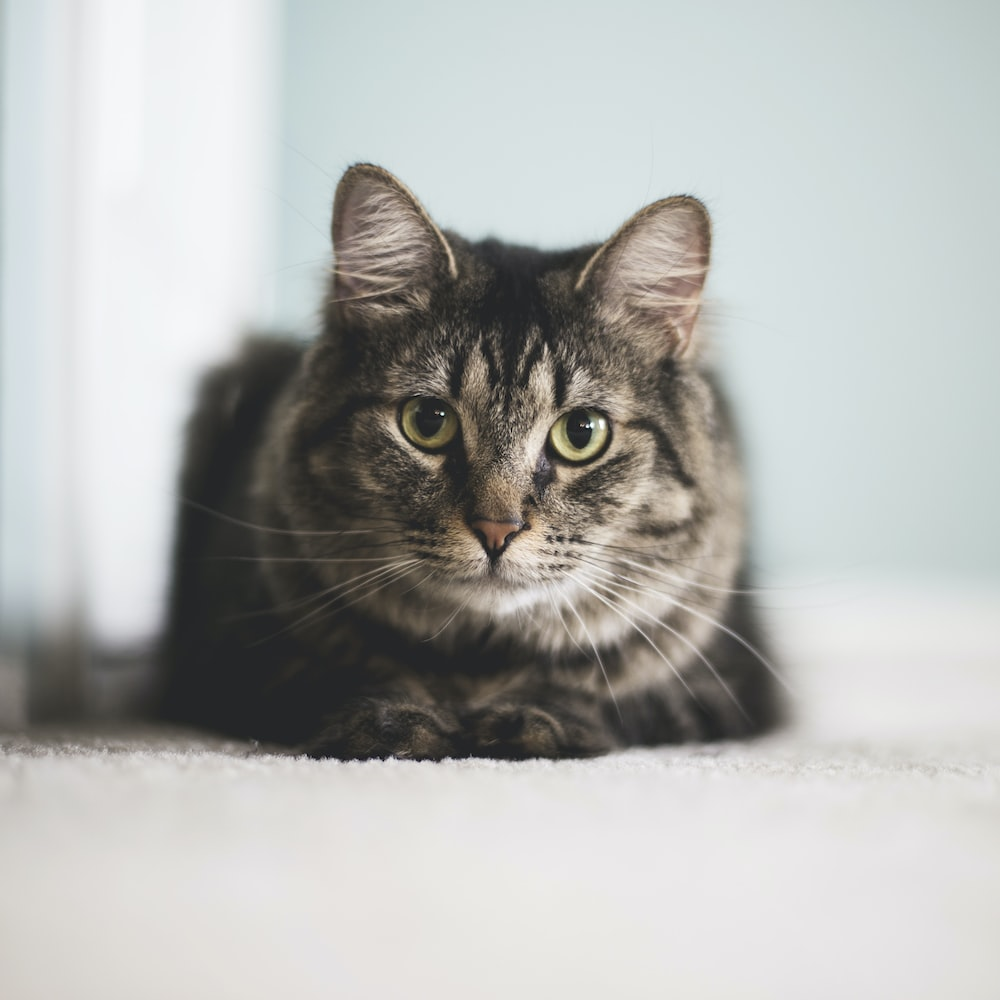
\includegraphics[width=1cm]{data/cat.jpeg}
			};

			\matrix[every node/.style={minimum height=0.15cm, minimum width=0.15cm, draw=black, fill=nodefill, inner sep=0pt}] at (1.65, 0.1) {
				\node{}; \& \node{}; \& \node{}; \& \node{}; \& \node{}; \& \node{}; \& \node{}; \& \node{};\\
				\node{}; \& \node{}; \& \node{}; \& \node{}; \& \node{}; \& \node{}; \& \node{}; \& \node{};\\
				\node{}; \& \node{}; \& \node{}; \& \node{}; \& \node{}; \& \node{}; \& \node{}; \& \node{};\\
				\node{}; \& \node{}; \& \node{}; \& \node{}; \& \node{}; \& \node{}; \& \node{}; \& \node{};\\
				\node{}; \& \node{}; \& \node{}; \& \node{}; \& \node{}; \& \node{}; \& \node{}; \& \node{};\\
				\node{}; \& \node{}; \& \node{}; \& \node{}; \& \node{}; \& \node{}; \& \node{}; \& \node{};\\
				\node{}; \& \node{}; \& \node{}; \& \node{}; \& \node{}; \& \node{}; \& \node{}; \& \node{};\\
				\node{}; \& \node{}; \& \node{}; \& \node{}; \& \node{}; \& \node{}; \& \node{}; \& \node{};\\
			};

			\matrix[every node/.style={minimum height=0.15cm, minimum width=0.15cm, draw=black, fill=nodefill, inner sep=0pt, outer sep=0pt}] (l1) at (1.75, 0) {
				\node{}; \& \node{}; \& \node{}; \& \node{}; \& \node{}; \& \node{}; \& \node{}; \& \node{};\\
				\node{}; \& \node{}; \& \node{}; \& \node{}; \& \node{}; \& \node{}; \& \node{}; \& \node{};\\
				\node{}; \& \node{}; \& \node{}; \& \node{}; \& \node{}; \& \node{}; \& \node{}; \& \node{};\\
				\node{}; \& \node{}; \& \node{}; \& \node{}; \& \node{}; \& \node{}; \& \node{}; \& \node{};\\
				\node{}; \& \node{}; \& \node{}; \& \node{}; \& \node{}; \& \node{}; \& \node{}; \& \node{};\\
				\node{}; \& \node{}; \& \node{}; \& \node{}; \& \node{}; \& \node{}; \& \node{}; \& \node{};\\
				\node{}; \& \node{}; \& \node{}; \& \node{}; \& \node{}; \& \node{}; \& \node{}; \& \node{};\\
				\node{}; \& \node{}; \& \node{}; \& \node{}; \& \node{}; \& \node{}; \& \node{}; \& \node{};\\
			};
			\draw[->] (l0) -- (l1);

			\matrix[every node/.style={minimum height=0.15cm, minimum width=0.15cm, draw=black, fill=nodefill, inner sep=0pt}] at (1.85, -0.1) {
				\node{}; \& \node{}; \& \node{}; \& \node{}; \& \node{}; \& \node{}; \& \node{}; \& \node{};\\
				\node{}; \& \node{}; \& \node{}; \& \node{}; \& \node{}; \& \node{}; \& \node{}; \& \node{};\\
				\node{}; \& \node{}; \& \node{}; \& \node{}; \& \node{}; \& \node{}; \& \node{}; \& \node{};\\
				\node{}; \& \node{}; \& \node{}; \& \node{}; \& \node{}; \& \node{}; \& \node{}; \& \node{};\\
				\node{}; \& \node{}; \& \node{}; \& \node{}; \& \node{}; \& \node{}; \& \node{}; \& \node{};\\
				\node{}; \& \node{}; \& \node{}; \& \node{}; \& \node{}; \& \node{}; \& \node{}; \& \node{};\\
				\node{}; \& \node{}; \& \node{}; \& \node{}; \& \node{}; \& \node{}; \& \node{}; \& \node{};\\
				\node{}; \& \node{}; \& \node{}; \& \node{}; \& \node{}; \& \node{}; \& \node{}; \& \node{};\\
			};

			\matrix[every node/.style={minimum height=0.15cm, minimum width=0.15cm, draw=black, fill=nodefill, inner sep=0pt}] at (3.4, 0.1) {
				\node{}; \& \node{}; \& \node{}; \& \node{}; \& \node{}; \& \node{};\\
				\node{}; \& \node{}; \& \node{}; \& \node{}; \& \node{}; \& \node{};\\
				\node{}; \& \node{}; \& \node{}; \& \node{}; \& \node{}; \& \node{};\\
				\node{}; \& \node{}; \& \node{}; \& \node{}; \& \node{}; \& \node{};\\
				\node{}; \& \node{}; \& \node{}; \& \node{}; \& \node{}; \& \node{};\\
				\node{}; \& \node{}; \& \node{}; \& \node{}; \& \node{}; \& \node{};\\
			};

			\matrix[every node/.style={minimum height=0.15cm, minimum width=0.15cm, draw=black, fill=nodefill, inner sep=0pt}] (l2)at (3.5, 0) {
				\node{}; \& \node{}; \& \node{}; \& \node{}; \& \node{}; \& \node{};\\
				\node{}; \& \node{}; \& \node{}; \& \node{}; \& \node{}; \& \node{};\\
				\node{}; \& \node{}; \& \node{}; \& \node{}; \& \node{}; \& \node{};\\
				\node{}; \& \node{}; \& \node{}; \& \node{}; \& \node{}; \& \node{};\\
				\node{}; \& \node{}; \& \node{}; \& \node{}; \& \node{}; \& \node{};\\
				\node{}; \& \node{}; \& \node{}; \& \node{}; \& \node{}; \& \node{};\\
			};
			\draw[->] (l1) -- (l2);

			\matrix[every node/.style={minimum height=0.15cm, minimum width=0.15cm, draw=black, fill=nodefill, inner sep=0pt}] at (3.6, -0.1) {
				\node{}; \& \node{}; \& \node{}; \& \node{}; \& \node{}; \& \node{};\\
				\node{}; \& \node{}; \& \node{}; \& \node{}; \& \node{}; \& \node{};\\
				\node{}; \& \node{}; \& \node{}; \& \node{}; \& \node{}; \& \node{};\\
				\node{}; \& \node{}; \& \node{}; \& \node{}; \& \node{}; \& \node{};\\
				\node{}; \& \node{}; \& \node{}; \& \node{}; \& \node{}; \& \node{};\\
				\node{}; \& \node{}; \& \node{}; \& \node{}; \& \node{}; \& \node{};\\
			};

			\matrix[every node/.style={minimum height=0.15cm, minimum width=0.15cm, draw=black, fill=nodefill, inner sep=0pt}] at (5.05, 0.2) {
				\node{}; \& \node{}; \& \node{}; \& \node{}; \& \node{}; \& \node{};\\
				\node{}; \& \node{}; \& \node{}; \& \node{}; \& \node{}; \& \node{};\\
				\node{}; \& \node{}; \& \node{}; \& \node{}; \& \node{}; \& \node{};\\
				\node{}; \& \node{}; \& \node{}; \& \node{}; \& \node{}; \& \node{};\\
				\node{}; \& \node{}; \& \node{}; \& \node{}; \& \node{}; \& \node{};\\
				\node{}; \& \node{}; \& \node{}; \& \node{}; \& \node{}; \& \node{};\\
			};

			\matrix[every node/.style={minimum height=0.15cm, minimum width=0.15cm, draw=black, fill=nodefill, inner sep=0pt}] at (5.15, 0.1) {
				\node{}; \& \node{}; \& \node{}; \& \node{}; \& \node{}; \& \node{};\\
				\node{}; \& \node{}; \& \node{}; \& \node{}; \& \node{}; \& \node{};\\
				\node{}; \& \node{}; \& \node{}; \& \node{}; \& \node{}; \& \node{};\\
				\node{}; \& \node{}; \& \node{}; \& \node{}; \& \node{}; \& \node{};\\
				\node{}; \& \node{}; \& \node{}; \& \node{}; \& \node{}; \& \node{};\\
				\node{}; \& \node{}; \& \node{}; \& \node{}; \& \node{}; \& \node{};\\
			};

			\matrix[every node/.style={minimum height=0.15cm, minimum width=0.15cm, draw=black, fill=nodefill, inner sep=0pt}] (l3) at (5.25, 0) {
				\node{}; \& \node{}; \& \node{}; \& \node{}; \& \node{}; \& \node{};\\
				\node{}; \& \node{}; \& \node{}; \& \node{}; \& \node{}; \& \node{};\\
				\node{}; \& \node{}; \& \node{}; \& \node{}; \& \node{}; \& \node{};\\
				\node{}; \& \node{}; \& \node{}; \& \node{}; \& \node{}; \& \node{};\\
				\node{}; \& \node{}; \& \node{}; \& \node{}; \& \node{}; \& \node{};\\
				\node{}; \& \node{}; \& \node{}; \& \node{}; \& \node{}; \& \node{};\\
			};
			\draw[->] (l2) -- ($ (l3.west) - (0.1, 0) $);

			\matrix[every node/.style={minimum height=0.15cm, minimum width=0.15cm, draw=black, fill=nodefill, inner sep=0pt}] at (5.35, -0.1) {
				\node{}; \& \node{}; \& \node{}; \& \node{}; \& \node{}; \& \node{};\\
				\node{}; \& \node{}; \& \node{}; \& \node{}; \& \node{}; \& \node{};\\
				\node{}; \& \node{}; \& \node{}; \& \node{}; \& \node{}; \& \node{};\\
				\node{}; \& \node{}; \& \node{}; \& \node{}; \& \node{}; \& \node{};\\
				\node{}; \& \node{}; \& \node{}; \& \node{}; \& \node{}; \& \node{};\\
				\node{}; \& \node{}; \& \node{}; \& \node{}; \& \node{}; \& \node{};\\
			};

			\matrix[every node/.style={minimum height=0.15cm, minimum width=0.15cm, draw=black, fill=nodefill, inner sep=0pt}] at (5.45, -0.2) {
				\node{}; \& \node{}; \& \node{}; \& \node{}; \& \node{}; \& \node{};\\
				\node{}; \& \node{}; \& \node{}; \& \node{}; \& \node{}; \& \node{};\\
				\node{}; \& \node{}; \& \node{}; \& \node{}; \& \node{}; \& \node{};\\
				\node{}; \& \node{}; \& \node{}; \& \node{}; \& \node{}; \& \node{};\\
				\node{}; \& \node{}; \& \node{}; \& \node{}; \& \node{}; \& \node{};\\
				\node{}; \& \node{}; \& \node{}; \& \node{}; \& \node{}; \& \node{};\\
			};

			\matrix[every node/.style={minimum height=0.15cm, minimum width=0.15cm, draw=black, fill=nodefill, inner sep=0pt}] at (6.8, 0.2) {
				\node{}; \& \node{}; \& \node{}; \& \node{};\\
				\node{}; \& \node{}; \& \node{}; \& \node{};\\
				\node{}; \& \node{}; \& \node{}; \& \node{};\\
				\node{}; \& \node{}; \& \node{}; \& \node{};\\
			};

			\matrix[every node/.style={minimum height=0.15cm, minimum width=0.15cm, draw=black, fill=nodefill, inner sep=0pt}] at (6.9, 0.1) {
				\node{}; \& \node{}; \& \node{}; \& \node{};\\
				\node{}; \& \node{}; \& \node{}; \& \node{};\\
				\node{}; \& \node{}; \& \node{}; \& \node{};\\
				\node{}; \& \node{}; \& \node{}; \& \node{};\\
			};

			\matrix[every node/.style={minimum height=0.15cm, minimum width=0.15cm, draw=black, fill=nodefill, inner sep=0pt}] (l4) at (7, 0) {
				\node{}; \& \node{}; \& \node{}; \& \node{};\\
				\node{}; \& \node{}; \& \node{}; \& \node{};\\
				\node{}; \& \node{}; \& \node{}; \& \node{};\\
				\node{}; \& \node{}; \& \node{}; \& \node{};\\
			};
			\draw[->] ($ (l3.east) + (0.1, 0) $) -- ($ (l4.west) + (-0.1, 0) $);

			\matrix[every node/.style={minimum height=0.15cm, minimum width=0.15cm, draw=black, fill=nodefill, inner sep=0pt}] at (7.1, -0.1) {
				\node{}; \& \node{}; \& \node{}; \& \node{};\\
				\node{}; \& \node{}; \& \node{}; \& \node{};\\
				\node{}; \& \node{}; \& \node{}; \& \node{};\\
				\node{}; \& \node{}; \& \node{}; \& \node{};\\
			};
			\matrix[every node/.style={minimum height=0.15cm, minimum width=0.15cm, draw=black, fill=nodefill, inner sep=0pt}] at (7.2, -0.2) {
				\node{}; \& \node{}; \& \node{}; \& \node{};\\
				\node{}; \& \node{}; \& \node{}; \& \node{};\\
				\node{}; \& \node{}; \& \node{}; \& \node{};\\
				\node{}; \& \node{}; \& \node{}; \& \node{};\\
			};

			\matrix[every node/.style={minimum height=0.15cm, minimum width=0.15cm, draw=black, fill=nodefill, inner sep=0pt}] at (8.25, 0.3) {
				\node{}; \& \node{}; \& \node{}; \& \node{};\\
				\node{}; \& \node{}; \& \node{}; \& \node{};\\
				\node{}; \& \node{}; \& \node{}; \& \node{};\\
				\node{}; \& \node{}; \& \node{}; \& \node{};\\
			};

			\matrix[every node/.style={minimum height=0.15cm, minimum width=0.15cm, draw=black, fill=nodefill, inner sep=0pt}] at (8.35, 0.2) {
				\node{}; \& \node{}; \& \node{}; \& \node{};\\
				\node{}; \& \node{}; \& \node{}; \& \node{};\\
				\node{}; \& \node{}; \& \node{}; \& \node{};\\
				\node{}; \& \node{}; \& \node{}; \& \node{};\\
			};

			\matrix[every node/.style={minimum height=0.15cm, minimum width=0.15cm, draw=black, fill=nodefill, inner sep=0pt}] at (8.45, 0.1) {
				\node{}; \& \node{}; \& \node{}; \& \node{};\\
				\node{}; \& \node{}; \& \node{}; \& \node{};\\
				\node{}; \& \node{}; \& \node{}; \& \node{};\\
				\node{}; \& \node{}; \& \node{}; \& \node{};\\
			};

			\matrix[every node/.style={minimum height=0.15cm, minimum width=0.15cm, draw=black, fill=nodefill, inner sep=0pt}] (l5) at (8.55, 0) {
				\node{}; \& \node{}; \& \node{}; \& \node{};\\
				\node{}; \& \node{}; \& \node{}; \& \node{};\\
				\node{}; \& \node{}; \& \node{}; \& \node{};\\
				\node{}; \& \node{}; \& \node{}; \& \node{};\\
			};
			\draw[->] ($ (l4.east) + (0.1, 0) $) -- ($ (l5.west) + (-0.2, 0) $);

			\matrix[every node/.style={minimum height=0.15cm, minimum width=0.15cm, draw=black, fill=nodefill, inner sep=0pt}] at (8.65, -0.1) {
				\node{}; \& \node{}; \& \node{}; \& \node{};\\
				\node{}; \& \node{}; \& \node{}; \& \node{};\\
				\node{}; \& \node{}; \& \node{}; \& \node{};\\
				\node{}; \& \node{}; \& \node{}; \& \node{};\\
			};

			\matrix[every node/.style={minimum height=0.15cm, minimum width=0.15cm, draw=black, fill=nodefill, inner sep=0pt}] at (8.75, -0.2) {
				\node{}; \& \node{}; \& \node{}; \& \node{};\\
				\node{}; \& \node{}; \& \node{}; \& \node{};\\
				\node{}; \& \node{}; \& \node{}; \& \node{};\\
				\node{}; \& \node{}; \& \node{}; \& \node{};\\
			};

			\matrix[every node/.style={minimum height=0.15cm, minimum width=0.15cm, draw=black, fill=nodefill, inner sep=0pt}] at (8.85, -0.3) {
				\node{}; \& \node{}; \& \node{}; \& \node{};\\
				\node{}; \& \node{}; \& \node{}; \& \node{};\\
				\node{}; \& \node{}; \& \node{}; \& \node{};\\
				\node{}; \& \node{}; \& \node{}; \& \node{};\\
			};


			\node[circle, draw=black, fill=nodefill, text depth=0, inner sep=2pt] (y1) at (10.5, 0.125) {\tiny{$y_0$}};
			\node[circle, draw=black, fill=nodefill, text depth=0, inner sep=2pt] (y2) at (10.75, -0.125) {\tiny{$y_1$}};

			\node[minimum height=0.15cm, minimum width=0.15cm, draw=black, fill=nodefill, inner sep=0pt] (n0) at (9.4, 0.3) {};
			\draw[->] (n0) -- (y1);
			\node[minimum height=0.15cm, minimum width=0.15cm, draw=black, fill=nodefill, inner sep=0pt] (n1) at (9.5, 0.2) {};
			\draw[->] (n1) -- (y1);
			\node[minimum height=0.15cm, minimum width=0.15cm, draw=black, fill=nodefill, inner sep=0pt] (n2) at (9.6, 0.1) {};
			\draw[->] (n2) -- (y1);
			\node[minimum height=0.15cm, minimum width=0.15cm, draw=black, fill=nodefill, inner sep=0pt] (n3) at (9.7, 0) {};
			\draw[->] ($ (l5.east) + (0.2, 0) $) -- ($ (n3.west) + (-0.15, 0) $);
			\draw[->] (n3) -- (y1);
			\node[minimum height=0.15cm, minimum width=0.15cm, draw=black, fill=nodefill, inner sep=0pt] (n4) at (9.8, -0.1) {};
			\draw[->] (n4) -- (y1);
			\node[minimum height=0.15cm, minimum width=0.15cm, draw=black, fill=nodefill, inner sep=0pt] (n5) at (9.9, -0.2) {};
			\draw[->] (n5) -- (y1);
			\node[minimum height=0.15cm, minimum width=0.15cm, draw=black, fill=nodefill, inner sep=0pt] (n6) at (10, -0.3) {};
			\draw[->] (n6) -- (y1);

			\node[minimum height=0.15cm, minimum width=0.15cm, draw=black, fill=nodefill, inner sep=0pt] (n0) at (9.4, 0.3) {};
			\draw[->] (n0) -- (y2);
			\node[minimum height=0.15cm, minimum width=0.15cm, draw=black, fill=nodefill, inner sep=0pt] (n1) at (9.5, 0.2) {};
			\draw[->] (n1) -- (y2);
			\node[minimum height=0.15cm, minimum width=0.15cm, draw=black, fill=nodefill, inner sep=0pt] (n2) at (9.6, 0.1) {};
			\draw[->] (n2) -- (y2);
			\node[minimum height=0.15cm, minimum width=0.15cm, draw=black, fill=nodefill, inner sep=0pt] (n3) at (9.7, 0) {};
			\draw[->] (n3) -- (y2);
			\node[minimum height=0.15cm, minimum width=0.15cm, draw=black, fill=nodefill, inner sep=0pt] (n4) at (9.8, -0.1) {};
			\draw[->] (n4) -- (y2);
			\node[minimum height=0.15cm, minimum width=0.15cm, draw=black, fill=nodefill, inner sep=0pt] (n5) at (9.9, -0.2) {};
			\draw[->] (n5) -- (y2);
			\node[minimum height=0.15cm, minimum width=0.15cm, draw=black, fill=nodefill, inner sep=0pt] (n6) at (10, -0.3) {};
			\draw[->] (n6) -- (y2);

			\node[] at (6, 3) {};
			\node[] at (11, -3) {};

		\end{tikzpicture}
		}
		\vfill
	\end{frame}

	\begin{frame}{Bildegjenkjenning: Konvolusjonelle nevrale nettverk} % Early
		\centering
		\vfill
		\resizebox{\textwidth}{!}{

		\colorlet{nodefill}{cyan!40}
		\begin{tikzpicture}[
			ampersand replacement=\&
		]
			\node[inner sep=0pt, draw=black] (l0) at (0, 0) {
				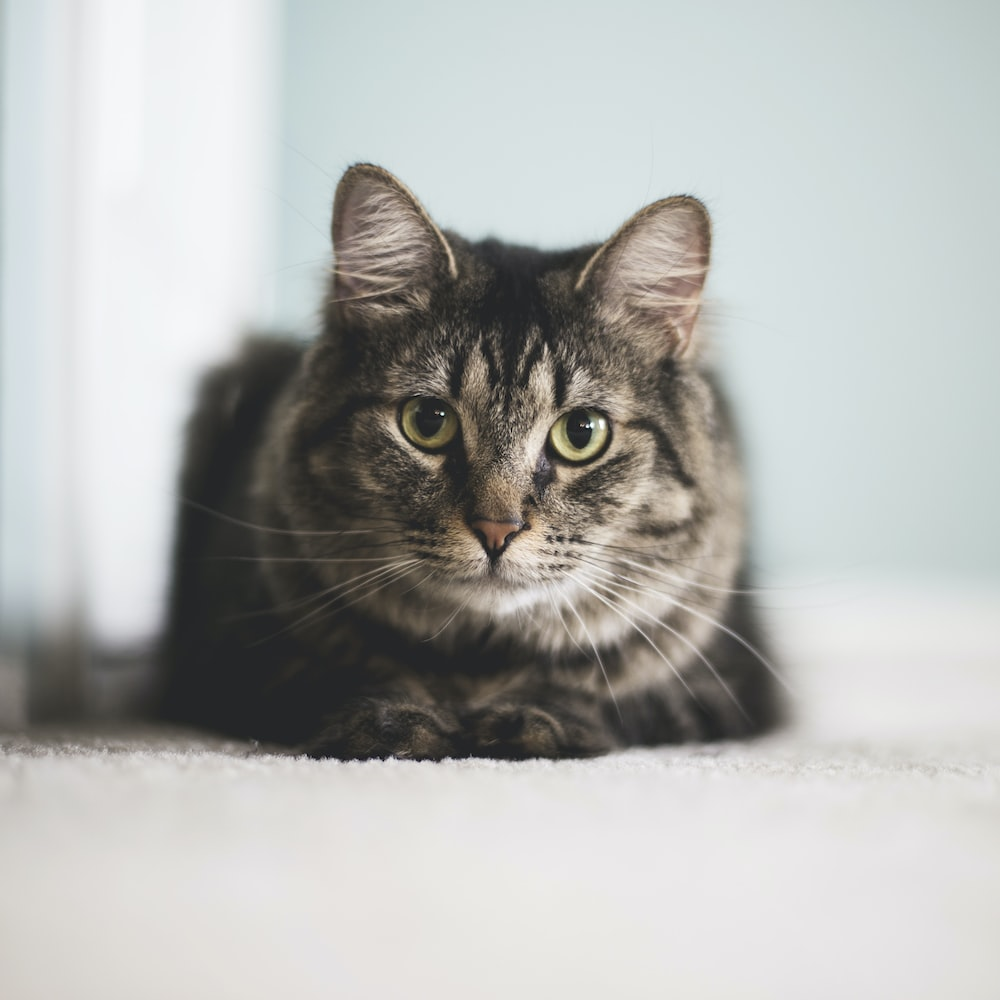
\includegraphics[width=1cm]{data/cat.jpeg}
			};

			\matrix[every node/.style={minimum height=0.15cm, minimum width=0.15cm, draw=black, fill=nodefill, inner sep=0pt}] at (1.65, 0.1) {
				\node{}; \& \node{}; \& \node{}; \& \node{}; \& \node{}; \& \node{}; \& \node{}; \& \node{};\\
				\node{}; \& \node{}; \& \node{}; \& \node{}; \& \node{}; \& \node{}; \& \node{}; \& \node{};\\
				\node{}; \& \node{}; \& \node{}; \& \node{}; \& \node{}; \& \node{}; \& \node{}; \& \node{};\\
				\node{}; \& \node{}; \& \node{}; \& \node{}; \& \node{}; \& \node{}; \& \node{}; \& \node{};\\
				\node{}; \& \node{}; \& \node{}; \& \node{}; \& \node{}; \& \node{}; \& \node{}; \& \node{};\\
				\node{}; \& \node{}; \& \node{}; \& \node{}; \& \node{}; \& \node{}; \& \node{}; \& \node{};\\
				\node{}; \& \node{}; \& \node{}; \& \node{}; \& \node{}; \& \node{}; \& \node{}; \& \node{};\\
				\node{}; \& \node{}; \& \node{}; \& \node{}; \& \node{}; \& \node{}; \& \node{}; \& \node{};\\
			};

			\matrix[every node/.style={minimum height=0.15cm, minimum width=0.15cm, draw=black, fill=nodefill, inner sep=0pt, outer sep=0pt}] (l1) at (1.75, 0) {
				\node{}; \& \node{}; \& \node{}; \& \node{}; \& \node{}; \& \node{}; \& \node{}; \& \node{};\\
				\node{}; \& \node{}; \& \node{}; \& \node{}; \& \node{}; \& \node{}; \& \node{}; \& \node{};\\
				\node{}; \& \node{}; \& \node{}; \& \node{}; \& \node{}; \& \node{}; \& \node{}; \& \node{};\\
				\node{}; \& \node{}; \& \node{}; \& \node{}; \& \node{}; \& \node{}; \& \node{}; \& \node{};\\
				\node{}; \& \node{}; \& \node{}; \& \node{}; \& \node{}; \& \node{}; \& \node{}; \& \node{};\\
				\node{}; \& \node{}; \& \node{}; \& \node{}; \& \node{}; \& \node{}; \& \node{}; \& \node{};\\
				\node{}; \& \node{}; \& \node{}; \& \node{}; \& \node{}; \& \node{}; \& \node{}; \& \node{};\\
				\node{}; \& \node{}; \& \node{}; \& \node{}; \& \node{}; \& \node{}; \& \node{}; \& \node{};\\
			};
			\draw[->] (l0) -- (l1);

			\matrix[every node/.style={minimum height=0.15cm, minimum width=0.15cm, draw=black, fill=nodefill, inner sep=0pt}] at (1.85, -0.1) {
				\node{}; \& \node{}; \& \node{}; \& \node{}; \& \node{}; \& \node{}; \& \node{}; \& \node{};\\
				\node{}; \& \node{}; \& \node{}; \& \node{}; \& \node{}; \& \node{}; \& \node{}; \& \node{};\\
				\node{}; \& \node{}; \& \node{}; \& \node{}; \& \node{}; \& \node{}; \& \node{}; \& \node{};\\
				\node{}; \& \node{}; \& \node{}; \& \node{}; \& \node{}; \& \node{}; \& \node{}; \& \node{};\\
				\node{}; \& \node{}; \& \node{}; \& \node{}; \& \node{}; \& \node{}; \& \node{}; \& \node{};\\
				\node{}; \& \node{}; \& \node{}; \& \node{}; \& \node{}; \& \node{}; \& \node{}; \& \node{};\\
				\node{}; \& \node{}; \& \node{}; \& \node{}; \& \node{}; \& \node{}; \& \node{}; \& \node{};\\
				\node{}; \& \node{}; \& \node{}; \& \node{}; \& \node{}; \& \node{}; \& \node{}; \& \node{};\\
			};

			\matrix[every node/.style={minimum height=0.15cm, minimum width=0.15cm, draw=black, fill=nodefill, inner sep=0pt}] at (3.4, 0.1) {
				\node{}; \& \node{}; \& \node{}; \& \node{}; \& \node{}; \& \node{};\\
				\node{}; \& \node{}; \& \node{}; \& \node{}; \& \node{}; \& \node{};\\
				\node{}; \& \node{}; \& \node{}; \& \node{}; \& \node{}; \& \node{};\\
				\node{}; \& \node{}; \& \node{}; \& \node{}; \& \node{}; \& \node{};\\
				\node{}; \& \node{}; \& \node{}; \& \node{}; \& \node{}; \& \node{};\\
				\node{}; \& \node{}; \& \node{}; \& \node{}; \& \node{}; \& \node{};\\
			};

			\matrix[every node/.style={minimum height=0.15cm, minimum width=0.15cm, draw=black, fill=nodefill, inner sep=0pt}] (l2)at (3.5, 0) {
				\node{}; \& \node{}; \& \node{}; \& \node{}; \& \node{}; \& \node{};\\
				\node{}; \& \node{}; \& \node{}; \& \node{}; \& \node{}; \& \node{};\\
				\node{}; \& \node{}; \& \node{}; \& \node{}; \& \node{}; \& \node{};\\
				\node{}; \& \node{}; \& \node{}; \& \node{}; \& \node{}; \& \node{};\\
				\node{}; \& \node{}; \& \node{}; \& \node{}; \& \node{}; \& \node{};\\
				\node{}; \& \node{}; \& \node{}; \& \node{}; \& \node{}; \& \node{};\\
			};
			\draw[->] (l1) -- (l2);

			\matrix[every node/.style={minimum height=0.15cm, minimum width=0.15cm, draw=black, fill=nodefill, inner sep=0pt}] at (3.6, -0.1) {
				\node{}; \& \node{}; \& \node{}; \& \node{}; \& \node{}; \& \node{};\\
				\node{}; \& \node{}; \& \node{}; \& \node{}; \& \node{}; \& \node{};\\
				\node{}; \& \node{}; \& \node{}; \& \node{}; \& \node{}; \& \node{};\\
				\node{}; \& \node{}; \& \node{}; \& \node{}; \& \node{}; \& \node{};\\
				\node{}; \& \node{}; \& \node{}; \& \node{}; \& \node{}; \& \node{};\\
				\node{}; \& \node{}; \& \node{}; \& \node{}; \& \node{}; \& \node{};\\
			};

			\matrix[every node/.style={minimum height=0.15cm, minimum width=0.15cm, draw=black, fill=nodefill, inner sep=0pt}] at (5.05, 0.2) {
				\node{}; \& \node{}; \& \node{}; \& \node{}; \& \node{}; \& \node{};\\
				\node{}; \& \node{}; \& \node{}; \& \node{}; \& \node{}; \& \node{};\\
				\node{}; \& \node{}; \& \node{}; \& \node{}; \& \node{}; \& \node{};\\
				\node{}; \& \node{}; \& \node{}; \& \node{}; \& \node{}; \& \node{};\\
				\node{}; \& \node{}; \& \node{}; \& \node{}; \& \node{}; \& \node{};\\
				\node{}; \& \node{}; \& \node{}; \& \node{}; \& \node{}; \& \node{};\\
			};

			\matrix[every node/.style={minimum height=0.15cm, minimum width=0.15cm, draw=black, fill=nodefill, inner sep=0pt}] at (5.15, 0.1) {
				\node{}; \& \node{}; \& \node{}; \& \node{}; \& \node{}; \& \node{};\\
				\node{}; \& \node{}; \& \node{}; \& \node{}; \& \node{}; \& \node{};\\
				\node{}; \& \node{}; \& \node{}; \& \node{}; \& \node{}; \& \node{};\\
				\node{}; \& \node{}; \& \node{}; \& \node{}; \& \node{}; \& \node{};\\
				\node{}; \& \node{}; \& \node{}; \& \node{}; \& \node{}; \& \node{};\\
				\node{}; \& \node{}; \& \node{}; \& \node{}; \& \node{}; \& \node{};\\
			};

			\matrix[every node/.style={minimum height=0.15cm, minimum width=0.15cm, draw=black, fill=nodefill, inner sep=0pt}] (l3) at (5.25, 0) {
				\node{}; \& \node{}; \& \node{}; \& \node{}; \& \node{}; \& \node{};\\
				\node{}; \& \node{}; \& \node{}; \& \node{}; \& \node{}; \& \node{};\\
				\node{}; \& \node{}; \& \node{}; \& \node{}; \& \node{}; \& \node{};\\
				\node{}; \& \node{}; \& \node{}; \& \node{}; \& \node{}; \& \node{};\\
				\node{}; \& \node{}; \& \node{}; \& \node{}; \& \node{}; \& \node{};\\
				\node{}; \& \node{}; \& \node{}; \& \node{}; \& \node{}; \& \node{};\\
			};
			\draw[->] (l2) -- ($ (l3.west) - (0.1, 0) $);

			\matrix[every node/.style={minimum height=0.15cm, minimum width=0.15cm, draw=black, fill=nodefill, inner sep=0pt}] at (5.35, -0.1) {
				\node{}; \& \node{}; \& \node{}; \& \node{}; \& \node{}; \& \node{};\\
				\node{}; \& \node{}; \& \node{}; \& \node{}; \& \node{}; \& \node{};\\
				\node{}; \& \node{}; \& \node{}; \& \node{}; \& \node{}; \& \node{};\\
				\node{}; \& \node{}; \& \node{}; \& \node{}; \& \node{}; \& \node{};\\
				\node{}; \& \node{}; \& \node{}; \& \node{}; \& \node{}; \& \node{};\\
				\node{}; \& \node{}; \& \node{}; \& \node{}; \& \node{}; \& \node{};\\
			};

			\matrix[every node/.style={minimum height=0.15cm, minimum width=0.15cm, draw=black, fill=nodefill, inner sep=0pt}] at (5.45, -0.2) {
				\node{}; \& \node{}; \& \node{}; \& \node{}; \& \node{}; \& \node{};\\
				\node{}; \& \node{}; \& \node{}; \& \node{}; \& \node{}; \& \node{};\\
				\node{}; \& \node{}; \& \node{}; \& \node{}; \& \node{}; \& \node{};\\
				\node{}; \& \node{}; \& \node{}; \& \node{}; \& \node{}; \& \node{};\\
				\node{}; \& \node{}; \& \node{}; \& \node{}; \& \node{}; \& \node{};\\
				\node{}; \& \node{}; \& \node{}; \& \node{}; \& \node{}; \& \node{};\\
			};

			\matrix[every node/.style={minimum height=0.15cm, minimum width=0.15cm, draw=black, fill=nodefill, inner sep=0pt}] at (6.8, 0.2) {
				\node{}; \& \node{}; \& \node{}; \& \node{};\\
				\node{}; \& \node{}; \& \node{}; \& \node{};\\
				\node{}; \& \node{}; \& \node{}; \& \node{};\\
				\node{}; \& \node{}; \& \node{}; \& \node{};\\
			};

			\matrix[every node/.style={minimum height=0.15cm, minimum width=0.15cm, draw=black, fill=nodefill, inner sep=0pt}] at (6.9, 0.1) {
				\node{}; \& \node{}; \& \node{}; \& \node{};\\
				\node{}; \& \node{}; \& \node{}; \& \node{};\\
				\node{}; \& \node{}; \& \node{}; \& \node{};\\
				\node{}; \& \node{}; \& \node{}; \& \node{};\\
			};

			\matrix[every node/.style={minimum height=0.15cm, minimum width=0.15cm, draw=black, fill=nodefill, inner sep=0pt}] (l4) at (7, 0) {
				\node{}; \& \node{}; \& \node{}; \& \node{};\\
				\node{}; \& \node{}; \& \node{}; \& \node{};\\
				\node{}; \& \node{}; \& \node{}; \& \node{};\\
				\node{}; \& \node{}; \& \node{}; \& \node{};\\
			};
			\draw[->] ($ (l3.east) + (0.1, 0) $) -- ($ (l4.west) + (-0.1, 0) $);

			\matrix[every node/.style={minimum height=0.15cm, minimum width=0.15cm, draw=black, fill=nodefill, inner sep=0pt}] at (7.1, -0.1) {
				\node{}; \& \node{}; \& \node{}; \& \node{};\\
				\node{}; \& \node{}; \& \node{}; \& \node{};\\
				\node{}; \& \node{}; \& \node{}; \& \node{};\\
				\node{}; \& \node{}; \& \node{}; \& \node{};\\
			};
			\matrix[every node/.style={minimum height=0.15cm, minimum width=0.15cm, draw=black, fill=nodefill, inner sep=0pt}] at (7.2, -0.2) {
				\node{}; \& \node{}; \& \node{}; \& \node{};\\
				\node{}; \& \node{}; \& \node{}; \& \node{};\\
				\node{}; \& \node{}; \& \node{}; \& \node{};\\
				\node{}; \& \node{}; \& \node{}; \& \node{};\\
			};

			\matrix[every node/.style={minimum height=0.15cm, minimum width=0.15cm, draw=black, fill=nodefill, inner sep=0pt}] at (8.25, 0.3) {
				\node{}; \& \node{}; \& \node{}; \& \node{};\\
				\node{}; \& \node{}; \& \node{}; \& \node{};\\
				\node{}; \& \node{}; \& \node{}; \& \node{};\\
				\node{}; \& \node{}; \& \node{}; \& \node{};\\
			};

			\matrix[every node/.style={minimum height=0.15cm, minimum width=0.15cm, draw=black, fill=nodefill, inner sep=0pt}] at (8.35, 0.2) {
				\node{}; \& \node{}; \& \node{}; \& \node{};\\
				\node{}; \& \node{}; \& \node{}; \& \node{};\\
				\node{}; \& \node{}; \& \node{}; \& \node{};\\
				\node{}; \& \node{}; \& \node{}; \& \node{};\\
			};

			\matrix[every node/.style={minimum height=0.15cm, minimum width=0.15cm, draw=black, fill=nodefill, inner sep=0pt}] at (8.45, 0.1) {
				\node{}; \& \node{}; \& \node{}; \& \node{};\\
				\node{}; \& \node{}; \& \node{}; \& \node{};\\
				\node{}; \& \node{}; \& \node{}; \& \node{};\\
				\node{}; \& \node{}; \& \node{}; \& \node{};\\
			};

			\matrix[every node/.style={minimum height=0.15cm, minimum width=0.15cm, draw=black, fill=nodefill, inner sep=0pt}] (l5) at (8.55, 0) {
				\node{}; \& \node{}; \& \node{}; \& \node{};\\
				\node{}; \& \node{}; \& \node{}; \& \node{};\\
				\node{}; \& \node{}; \& \node{}; \& \node{};\\
				\node{}; \& \node{}; \& \node{}; \& \node{};\\
			};
			\draw[->] ($ (l4.east) + (0.1, 0) $) -- ($ (l5.west) + (-0.2, 0) $);

			\matrix[every node/.style={minimum height=0.15cm, minimum width=0.15cm, draw=black, fill=nodefill, inner sep=0pt}] at (8.65, -0.1) {
				\node{}; \& \node{}; \& \node{}; \& \node{};\\
				\node{}; \& \node{}; \& \node{}; \& \node{};\\
				\node{}; \& \node{}; \& \node{}; \& \node{};\\
				\node{}; \& \node{}; \& \node{}; \& \node{};\\
			};

			\matrix[every node/.style={minimum height=0.15cm, minimum width=0.15cm, draw=black, fill=nodefill, inner sep=0pt}] at (8.75, -0.2) {
				\node{}; \& \node{}; \& \node{}; \& \node{};\\
				\node{}; \& \node{}; \& \node{}; \& \node{};\\
				\node{}; \& \node{}; \& \node{}; \& \node{};\\
				\node{}; \& \node{}; \& \node{}; \& \node{};\\
			};

			\matrix[every node/.style={minimum height=0.15cm, minimum width=0.15cm, draw=black, fill=nodefill, inner sep=0pt}] at (8.85, -0.3) {
				\node{}; \& \node{}; \& \node{}; \& \node{};\\
				\node{}; \& \node{}; \& \node{}; \& \node{};\\
				\node{}; \& \node{}; \& \node{}; \& \node{};\\
				\node{}; \& \node{}; \& \node{}; \& \node{};\\
			};


			\node[circle, draw=black, fill=nodefill, text depth=0, inner sep=2pt] (y1) at (10.5, 0.125) {\tiny{$y_0$}};
			\node[circle, draw=black, fill=nodefill, text depth=0, inner sep=2pt] (y2) at (10.75, -0.125) {\tiny{$y_1$}};

			\node[minimum height=0.15cm, minimum width=0.15cm, draw=black, fill=nodefill, inner sep=0pt] (n0) at (9.4, 0.3) {};
			\draw[->] (n0) -- (y1);
			\node[minimum height=0.15cm, minimum width=0.15cm, draw=black, fill=nodefill, inner sep=0pt] (n1) at (9.5, 0.2) {};
			\draw[->] (n1) -- (y1);
			\node[minimum height=0.15cm, minimum width=0.15cm, draw=black, fill=nodefill, inner sep=0pt] (n2) at (9.6, 0.1) {};
			\draw[->] (n2) -- (y1);
			\node[minimum height=0.15cm, minimum width=0.15cm, draw=black, fill=nodefill, inner sep=0pt] (n3) at (9.7, 0) {};
			\draw[->] ($ (l5.east) + (0.2, 0) $) -- ($ (n3.west) + (-0.15, 0) $);
			\draw[->] (n3) -- (y1);
			\node[minimum height=0.15cm, minimum width=0.15cm, draw=black, fill=nodefill, inner sep=0pt] (n4) at (9.8, -0.1) {};
			\draw[->] (n4) -- (y1);
			\node[minimum height=0.15cm, minimum width=0.15cm, draw=black, fill=nodefill, inner sep=0pt] (n5) at (9.9, -0.2) {};
			\draw[->] (n5) -- (y1);
			\node[minimum height=0.15cm, minimum width=0.15cm, draw=black, fill=nodefill, inner sep=0pt] (n6) at (10, -0.3) {};
			\draw[->] (n6) -- (y1);

			\node[minimum height=0.15cm, minimum width=0.15cm, draw=black, fill=nodefill, inner sep=0pt] (n0) at (9.4, 0.3) {};
			\draw[->] (n0) -- (y2);
			\node[minimum height=0.15cm, minimum width=0.15cm, draw=black, fill=nodefill, inner sep=0pt] (n1) at (9.5, 0.2) {};
			\draw[->] (n1) -- (y2);
			\node[minimum height=0.15cm, minimum width=0.15cm, draw=black, fill=nodefill, inner sep=0pt] (n2) at (9.6, 0.1) {};
			\draw[->] (n2) -- (y2);
			\node[minimum height=0.15cm, minimum width=0.15cm, draw=black, fill=nodefill, inner sep=0pt] (n3) at (9.7, 0) {};
			\draw[->] (n3) -- (y2);
			\node[minimum height=0.15cm, minimum width=0.15cm, draw=black, fill=nodefill, inner sep=0pt] (n4) at (9.8, -0.1) {};
			\draw[->] (n4) -- (y2);
			\node[minimum height=0.15cm, minimum width=0.15cm, draw=black, fill=nodefill, inner sep=0pt] (n5) at (9.9, -0.2) {};
			\draw[->] (n5) -- (y2);
			\node[minimum height=0.15cm, minimum width=0.15cm, draw=black, fill=nodefill, inner sep=0pt] (n6) at (10, -0.3) {};
			\draw[->] (n6) -- (y2);

			\node[] at (1.75, -2) {
				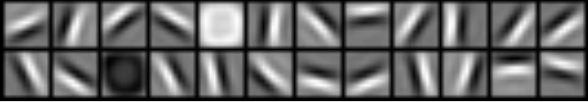
\includegraphics[width=3cm]{data/early.png}
			};

			\node[] at (6, 3) {};
			\node[] at (11, -3) {};

		\end{tikzpicture}
		}
		\vfill
	\end{frame}

	\begin{frame}{Bildegjenkjenning: Konvolusjonelle nevrale nettverk} % Intermediate
		\centering
		\vfill
		\resizebox{\textwidth}{!}{

		\colorlet{nodefill}{cyan!40}
		\begin{tikzpicture}[
			ampersand replacement=\&
		]
			\node[inner sep=0pt, draw=black] (l0) at (0, 0) {
				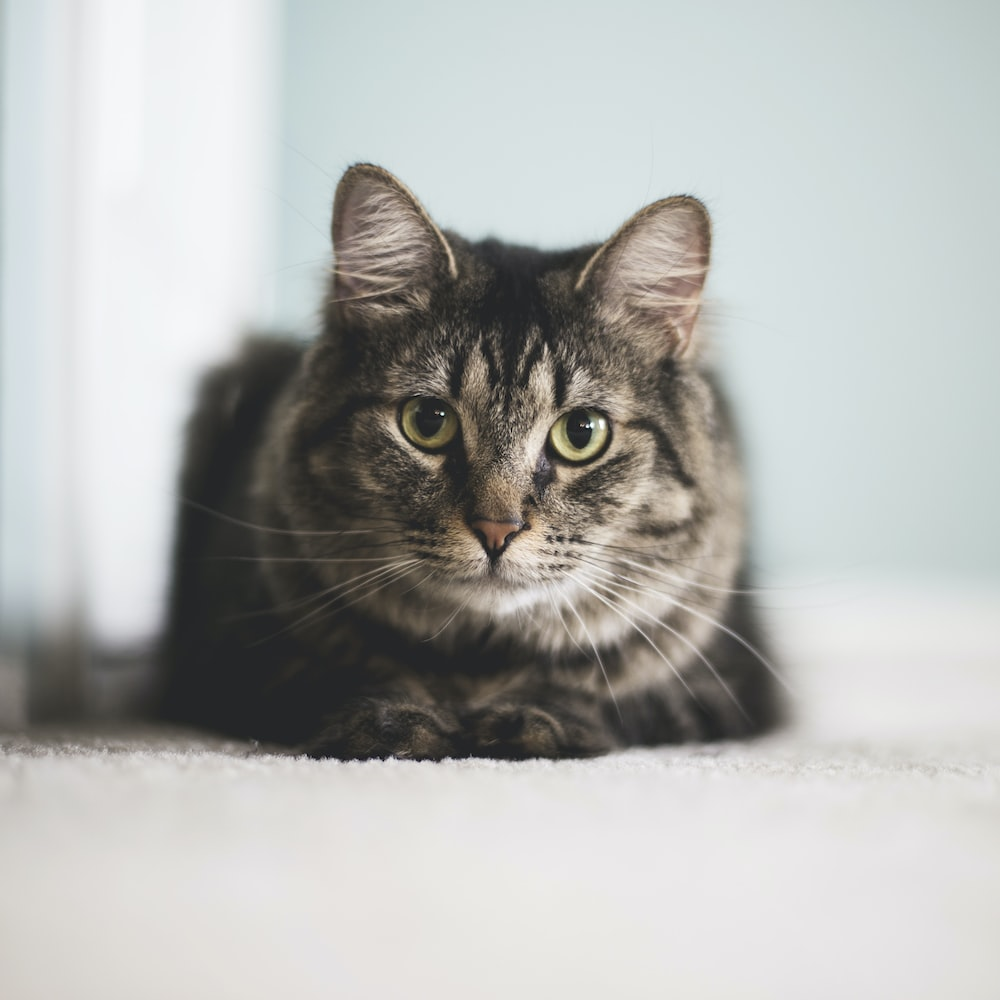
\includegraphics[width=1cm]{data/cat.jpeg}
			};

			\matrix[every node/.style={minimum height=0.15cm, minimum width=0.15cm, draw=black, fill=nodefill, inner sep=0pt}] at (1.65, 0.1) {
				\node{}; \& \node{}; \& \node{}; \& \node{}; \& \node{}; \& \node{}; \& \node{}; \& \node{};\\
				\node{}; \& \node{}; \& \node{}; \& \node{}; \& \node{}; \& \node{}; \& \node{}; \& \node{};\\
				\node{}; \& \node{}; \& \node{}; \& \node{}; \& \node{}; \& \node{}; \& \node{}; \& \node{};\\
				\node{}; \& \node{}; \& \node{}; \& \node{}; \& \node{}; \& \node{}; \& \node{}; \& \node{};\\
				\node{}; \& \node{}; \& \node{}; \& \node{}; \& \node{}; \& \node{}; \& \node{}; \& \node{};\\
				\node{}; \& \node{}; \& \node{}; \& \node{}; \& \node{}; \& \node{}; \& \node{}; \& \node{};\\
				\node{}; \& \node{}; \& \node{}; \& \node{}; \& \node{}; \& \node{}; \& \node{}; \& \node{};\\
				\node{}; \& \node{}; \& \node{}; \& \node{}; \& \node{}; \& \node{}; \& \node{}; \& \node{};\\
			};

			\matrix[every node/.style={minimum height=0.15cm, minimum width=0.15cm, draw=black, fill=nodefill, inner sep=0pt, outer sep=0pt}] (l1) at (1.75, 0) {
				\node{}; \& \node{}; \& \node{}; \& \node{}; \& \node{}; \& \node{}; \& \node{}; \& \node{};\\
				\node{}; \& \node{}; \& \node{}; \& \node{}; \& \node{}; \& \node{}; \& \node{}; \& \node{};\\
				\node{}; \& \node{}; \& \node{}; \& \node{}; \& \node{}; \& \node{}; \& \node{}; \& \node{};\\
				\node{}; \& \node{}; \& \node{}; \& \node{}; \& \node{}; \& \node{}; \& \node{}; \& \node{};\\
				\node{}; \& \node{}; \& \node{}; \& \node{}; \& \node{}; \& \node{}; \& \node{}; \& \node{};\\
				\node{}; \& \node{}; \& \node{}; \& \node{}; \& \node{}; \& \node{}; \& \node{}; \& \node{};\\
				\node{}; \& \node{}; \& \node{}; \& \node{}; \& \node{}; \& \node{}; \& \node{}; \& \node{};\\
				\node{}; \& \node{}; \& \node{}; \& \node{}; \& \node{}; \& \node{}; \& \node{}; \& \node{};\\
			};
			\draw[->] (l0) -- (l1);

			\matrix[every node/.style={minimum height=0.15cm, minimum width=0.15cm, draw=black, fill=nodefill, inner sep=0pt}] at (1.85, -0.1) {
				\node{}; \& \node{}; \& \node{}; \& \node{}; \& \node{}; \& \node{}; \& \node{}; \& \node{};\\
				\node{}; \& \node{}; \& \node{}; \& \node{}; \& \node{}; \& \node{}; \& \node{}; \& \node{};\\
				\node{}; \& \node{}; \& \node{}; \& \node{}; \& \node{}; \& \node{}; \& \node{}; \& \node{};\\
				\node{}; \& \node{}; \& \node{}; \& \node{}; \& \node{}; \& \node{}; \& \node{}; \& \node{};\\
				\node{}; \& \node{}; \& \node{}; \& \node{}; \& \node{}; \& \node{}; \& \node{}; \& \node{};\\
				\node{}; \& \node{}; \& \node{}; \& \node{}; \& \node{}; \& \node{}; \& \node{}; \& \node{};\\
				\node{}; \& \node{}; \& \node{}; \& \node{}; \& \node{}; \& \node{}; \& \node{}; \& \node{};\\
				\node{}; \& \node{}; \& \node{}; \& \node{}; \& \node{}; \& \node{}; \& \node{}; \& \node{};\\
			};

			\matrix[every node/.style={minimum height=0.15cm, minimum width=0.15cm, draw=black, fill=nodefill, inner sep=0pt}] at (3.4, 0.1) {
				\node{}; \& \node{}; \& \node{}; \& \node{}; \& \node{}; \& \node{};\\
				\node{}; \& \node{}; \& \node{}; \& \node{}; \& \node{}; \& \node{};\\
				\node{}; \& \node{}; \& \node{}; \& \node{}; \& \node{}; \& \node{};\\
				\node{}; \& \node{}; \& \node{}; \& \node{}; \& \node{}; \& \node{};\\
				\node{}; \& \node{}; \& \node{}; \& \node{}; \& \node{}; \& \node{};\\
				\node{}; \& \node{}; \& \node{}; \& \node{}; \& \node{}; \& \node{};\\
			};

			\matrix[every node/.style={minimum height=0.15cm, minimum width=0.15cm, draw=black, fill=nodefill, inner sep=0pt}] (l2)at (3.5, 0) {
				\node{}; \& \node{}; \& \node{}; \& \node{}; \& \node{}; \& \node{};\\
				\node{}; \& \node{}; \& \node{}; \& \node{}; \& \node{}; \& \node{};\\
				\node{}; \& \node{}; \& \node{}; \& \node{}; \& \node{}; \& \node{};\\
				\node{}; \& \node{}; \& \node{}; \& \node{}; \& \node{}; \& \node{};\\
				\node{}; \& \node{}; \& \node{}; \& \node{}; \& \node{}; \& \node{};\\
				\node{}; \& \node{}; \& \node{}; \& \node{}; \& \node{}; \& \node{};\\
			};
			\draw[->] (l1) -- (l2);

			\matrix[every node/.style={minimum height=0.15cm, minimum width=0.15cm, draw=black, fill=nodefill, inner sep=0pt}] at (3.6, -0.1) {
				\node{}; \& \node{}; \& \node{}; \& \node{}; \& \node{}; \& \node{};\\
				\node{}; \& \node{}; \& \node{}; \& \node{}; \& \node{}; \& \node{};\\
				\node{}; \& \node{}; \& \node{}; \& \node{}; \& \node{}; \& \node{};\\
				\node{}; \& \node{}; \& \node{}; \& \node{}; \& \node{}; \& \node{};\\
				\node{}; \& \node{}; \& \node{}; \& \node{}; \& \node{}; \& \node{};\\
				\node{}; \& \node{}; \& \node{}; \& \node{}; \& \node{}; \& \node{};\\
			};

			\matrix[every node/.style={minimum height=0.15cm, minimum width=0.15cm, draw=black, fill=nodefill, inner sep=0pt}] at (5.05, 0.2) {
				\node{}; \& \node{}; \& \node{}; \& \node{}; \& \node{}; \& \node{};\\
				\node{}; \& \node{}; \& \node{}; \& \node{}; \& \node{}; \& \node{};\\
				\node{}; \& \node{}; \& \node{}; \& \node{}; \& \node{}; \& \node{};\\
				\node{}; \& \node{}; \& \node{}; \& \node{}; \& \node{}; \& \node{};\\
				\node{}; \& \node{}; \& \node{}; \& \node{}; \& \node{}; \& \node{};\\
				\node{}; \& \node{}; \& \node{}; \& \node{}; \& \node{}; \& \node{};\\
			};

			\matrix[every node/.style={minimum height=0.15cm, minimum width=0.15cm, draw=black, fill=nodefill, inner sep=0pt}] at (5.15, 0.1) {
				\node{}; \& \node{}; \& \node{}; \& \node{}; \& \node{}; \& \node{};\\
				\node{}; \& \node{}; \& \node{}; \& \node{}; \& \node{}; \& \node{};\\
				\node{}; \& \node{}; \& \node{}; \& \node{}; \& \node{}; \& \node{};\\
				\node{}; \& \node{}; \& \node{}; \& \node{}; \& \node{}; \& \node{};\\
				\node{}; \& \node{}; \& \node{}; \& \node{}; \& \node{}; \& \node{};\\
				\node{}; \& \node{}; \& \node{}; \& \node{}; \& \node{}; \& \node{};\\
			};

			\matrix[every node/.style={minimum height=0.15cm, minimum width=0.15cm, draw=black, fill=nodefill, inner sep=0pt}] (l3) at (5.25, 0) {
				\node{}; \& \node{}; \& \node{}; \& \node{}; \& \node{}; \& \node{};\\
				\node{}; \& \node{}; \& \node{}; \& \node{}; \& \node{}; \& \node{};\\
				\node{}; \& \node{}; \& \node{}; \& \node{}; \& \node{}; \& \node{};\\
				\node{}; \& \node{}; \& \node{}; \& \node{}; \& \node{}; \& \node{};\\
				\node{}; \& \node{}; \& \node{}; \& \node{}; \& \node{}; \& \node{};\\
				\node{}; \& \node{}; \& \node{}; \& \node{}; \& \node{}; \& \node{};\\
			};
			\draw[->] (l2) -- ($ (l3.west) - (0.1, 0) $);

			\matrix[every node/.style={minimum height=0.15cm, minimum width=0.15cm, draw=black, fill=nodefill, inner sep=0pt}] at (5.35, -0.1) {
				\node{}; \& \node{}; \& \node{}; \& \node{}; \& \node{}; \& \node{};\\
				\node{}; \& \node{}; \& \node{}; \& \node{}; \& \node{}; \& \node{};\\
				\node{}; \& \node{}; \& \node{}; \& \node{}; \& \node{}; \& \node{};\\
				\node{}; \& \node{}; \& \node{}; \& \node{}; \& \node{}; \& \node{};\\
				\node{}; \& \node{}; \& \node{}; \& \node{}; \& \node{}; \& \node{};\\
				\node{}; \& \node{}; \& \node{}; \& \node{}; \& \node{}; \& \node{};\\
			};

			\matrix[every node/.style={minimum height=0.15cm, minimum width=0.15cm, draw=black, fill=nodefill, inner sep=0pt}] at (5.45, -0.2) {
				\node{}; \& \node{}; \& \node{}; \& \node{}; \& \node{}; \& \node{};\\
				\node{}; \& \node{}; \& \node{}; \& \node{}; \& \node{}; \& \node{};\\
				\node{}; \& \node{}; \& \node{}; \& \node{}; \& \node{}; \& \node{};\\
				\node{}; \& \node{}; \& \node{}; \& \node{}; \& \node{}; \& \node{};\\
				\node{}; \& \node{}; \& \node{}; \& \node{}; \& \node{}; \& \node{};\\
				\node{}; \& \node{}; \& \node{}; \& \node{}; \& \node{}; \& \node{};\\
			};

			\matrix[every node/.style={minimum height=0.15cm, minimum width=0.15cm, draw=black, fill=nodefill, inner sep=0pt}] at (6.8, 0.2) {
				\node{}; \& \node{}; \& \node{}; \& \node{};\\
				\node{}; \& \node{}; \& \node{}; \& \node{};\\
				\node{}; \& \node{}; \& \node{}; \& \node{};\\
				\node{}; \& \node{}; \& \node{}; \& \node{};\\
			};

			\matrix[every node/.style={minimum height=0.15cm, minimum width=0.15cm, draw=black, fill=nodefill, inner sep=0pt}] at (6.9, 0.1) {
				\node{}; \& \node{}; \& \node{}; \& \node{};\\
				\node{}; \& \node{}; \& \node{}; \& \node{};\\
				\node{}; \& \node{}; \& \node{}; \& \node{};\\
				\node{}; \& \node{}; \& \node{}; \& \node{};\\
			};

			\matrix[every node/.style={minimum height=0.15cm, minimum width=0.15cm, draw=black, fill=nodefill, inner sep=0pt}] (l4) at (7, 0) {
				\node{}; \& \node{}; \& \node{}; \& \node{};\\
				\node{}; \& \node{}; \& \node{}; \& \node{};\\
				\node{}; \& \node{}; \& \node{}; \& \node{};\\
				\node{}; \& \node{}; \& \node{}; \& \node{};\\
			};
			\draw[->] ($ (l3.east) + (0.1, 0) $) -- ($ (l4.west) + (-0.1, 0) $);

			\matrix[every node/.style={minimum height=0.15cm, minimum width=0.15cm, draw=black, fill=nodefill, inner sep=0pt}] at (7.1, -0.1) {
				\node{}; \& \node{}; \& \node{}; \& \node{};\\
				\node{}; \& \node{}; \& \node{}; \& \node{};\\
				\node{}; \& \node{}; \& \node{}; \& \node{};\\
				\node{}; \& \node{}; \& \node{}; \& \node{};\\
			};
			\matrix[every node/.style={minimum height=0.15cm, minimum width=0.15cm, draw=black, fill=nodefill, inner sep=0pt}] at (7.2, -0.2) {
				\node{}; \& \node{}; \& \node{}; \& \node{};\\
				\node{}; \& \node{}; \& \node{}; \& \node{};\\
				\node{}; \& \node{}; \& \node{}; \& \node{};\\
				\node{}; \& \node{}; \& \node{}; \& \node{};\\
			};

			\matrix[every node/.style={minimum height=0.15cm, minimum width=0.15cm, draw=black, fill=nodefill, inner sep=0pt}] at (8.25, 0.3) {
				\node{}; \& \node{}; \& \node{}; \& \node{};\\
				\node{}; \& \node{}; \& \node{}; \& \node{};\\
				\node{}; \& \node{}; \& \node{}; \& \node{};\\
				\node{}; \& \node{}; \& \node{}; \& \node{};\\
			};

			\matrix[every node/.style={minimum height=0.15cm, minimum width=0.15cm, draw=black, fill=nodefill, inner sep=0pt}] at (8.35, 0.2) {
				\node{}; \& \node{}; \& \node{}; \& \node{};\\
				\node{}; \& \node{}; \& \node{}; \& \node{};\\
				\node{}; \& \node{}; \& \node{}; \& \node{};\\
				\node{}; \& \node{}; \& \node{}; \& \node{};\\
			};

			\matrix[every node/.style={minimum height=0.15cm, minimum width=0.15cm, draw=black, fill=nodefill, inner sep=0pt}] at (8.45, 0.1) {
				\node{}; \& \node{}; \& \node{}; \& \node{};\\
				\node{}; \& \node{}; \& \node{}; \& \node{};\\
				\node{}; \& \node{}; \& \node{}; \& \node{};\\
				\node{}; \& \node{}; \& \node{}; \& \node{};\\
			};

			\matrix[every node/.style={minimum height=0.15cm, minimum width=0.15cm, draw=black, fill=nodefill, inner sep=0pt}] (l5) at (8.55, 0) {
				\node{}; \& \node{}; \& \node{}; \& \node{};\\
				\node{}; \& \node{}; \& \node{}; \& \node{};\\
				\node{}; \& \node{}; \& \node{}; \& \node{};\\
				\node{}; \& \node{}; \& \node{}; \& \node{};\\
			};
			\draw[->] ($ (l4.east) + (0.1, 0) $) -- ($ (l5.west) + (-0.2, 0) $);

			\matrix[every node/.style={minimum height=0.15cm, minimum width=0.15cm, draw=black, fill=nodefill, inner sep=0pt}] at (8.65, -0.1) {
				\node{}; \& \node{}; \& \node{}; \& \node{};\\
				\node{}; \& \node{}; \& \node{}; \& \node{};\\
				\node{}; \& \node{}; \& \node{}; \& \node{};\\
				\node{}; \& \node{}; \& \node{}; \& \node{};\\
			};

			\matrix[every node/.style={minimum height=0.15cm, minimum width=0.15cm, draw=black, fill=nodefill, inner sep=0pt}] at (8.75, -0.2) {
				\node{}; \& \node{}; \& \node{}; \& \node{};\\
				\node{}; \& \node{}; \& \node{}; \& \node{};\\
				\node{}; \& \node{}; \& \node{}; \& \node{};\\
				\node{}; \& \node{}; \& \node{}; \& \node{};\\
			};

			\matrix[every node/.style={minimum height=0.15cm, minimum width=0.15cm, draw=black, fill=nodefill, inner sep=0pt}] at (8.85, -0.3) {
				\node{}; \& \node{}; \& \node{}; \& \node{};\\
				\node{}; \& \node{}; \& \node{}; \& \node{};\\
				\node{}; \& \node{}; \& \node{}; \& \node{};\\
				\node{}; \& \node{}; \& \node{}; \& \node{};\\
			};


			\node[circle, draw=black, fill=nodefill, text depth=0, inner sep=2pt] (y1) at (10.5, 0.125) {\tiny{$y_0$}};
			\node[circle, draw=black, fill=nodefill, text depth=0, inner sep=2pt] (y2) at (10.75, -0.125) {\tiny{$y_1$}};

			\node[minimum height=0.15cm, minimum width=0.15cm, draw=black, fill=nodefill, inner sep=0pt] (n0) at (9.4, 0.3) {};
			\draw[->] (n0) -- (y1);
			\node[minimum height=0.15cm, minimum width=0.15cm, draw=black, fill=nodefill, inner sep=0pt] (n1) at (9.5, 0.2) {};
			\draw[->] (n1) -- (y1);
			\node[minimum height=0.15cm, minimum width=0.15cm, draw=black, fill=nodefill, inner sep=0pt] (n2) at (9.6, 0.1) {};
			\draw[->] (n2) -- (y1);
			\node[minimum height=0.15cm, minimum width=0.15cm, draw=black, fill=nodefill, inner sep=0pt] (n3) at (9.7, 0) {};
			\draw[->] ($ (l5.east) + (0.2, 0) $) -- ($ (n3.west) + (-0.15, 0) $);
			\draw[->] (n3) -- (y1);
			\node[minimum height=0.15cm, minimum width=0.15cm, draw=black, fill=nodefill, inner sep=0pt] (n4) at (9.8, -0.1) {};
			\draw[->] (n4) -- (y1);
			\node[minimum height=0.15cm, minimum width=0.15cm, draw=black, fill=nodefill, inner sep=0pt] (n5) at (9.9, -0.2) {};
			\draw[->] (n5) -- (y1);
			\node[minimum height=0.15cm, minimum width=0.15cm, draw=black, fill=nodefill, inner sep=0pt] (n6) at (10, -0.3) {};
			\draw[->] (n6) -- (y1);

			\node[minimum height=0.15cm, minimum width=0.15cm, draw=black, fill=nodefill, inner sep=0pt] (n0) at (9.4, 0.3) {};
			\draw[->] (n0) -- (y2);
			\node[minimum height=0.15cm, minimum width=0.15cm, draw=black, fill=nodefill, inner sep=0pt] (n1) at (9.5, 0.2) {};
			\draw[->] (n1) -- (y2);
			\node[minimum height=0.15cm, minimum width=0.15cm, draw=black, fill=nodefill, inner sep=0pt] (n2) at (9.6, 0.1) {};
			\draw[->] (n2) -- (y2);
			\node[minimum height=0.15cm, minimum width=0.15cm, draw=black, fill=nodefill, inner sep=0pt] (n3) at (9.7, 0) {};
			\draw[->] (n3) -- (y2);
			\node[minimum height=0.15cm, minimum width=0.15cm, draw=black, fill=nodefill, inner sep=0pt] (n4) at (9.8, -0.1) {};
			\draw[->] (n4) -- (y2);
			\node[minimum height=0.15cm, minimum width=0.15cm, draw=black, fill=nodefill, inner sep=0pt] (n5) at (9.9, -0.2) {};
			\draw[->] (n5) -- (y2);
			\node[minimum height=0.15cm, minimum width=0.15cm, draw=black, fill=nodefill, inner sep=0pt] (n6) at (10, -0.3) {};
			\draw[->] (n6) -- (y2);

			\node[] at (1.75, -2) {
				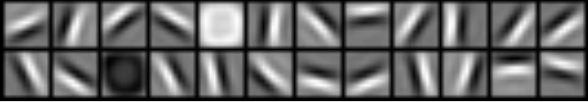
\includegraphics[width=3cm]{data/early.png}
			};

			\node[] at (5.25, -2) {
				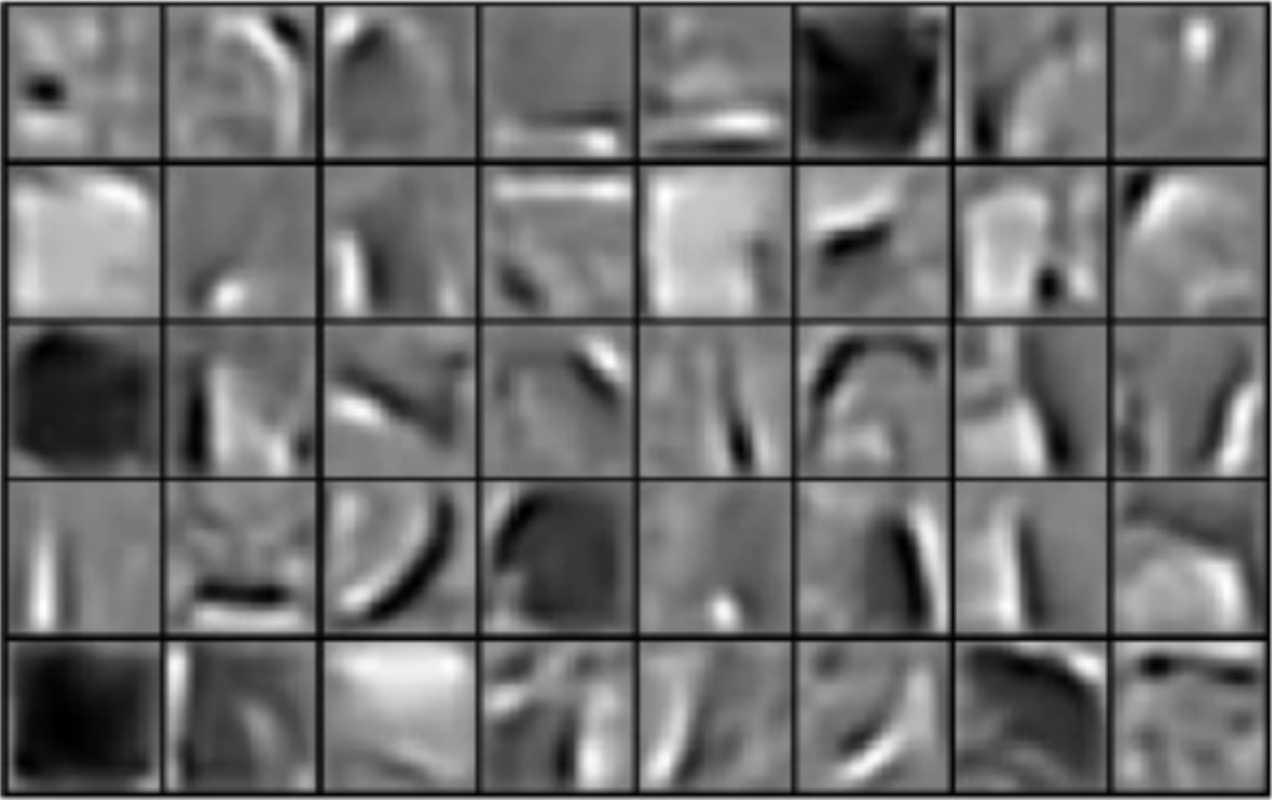
\includegraphics[width=3cm]{data/intermediate.png}
			};

			\node[] at (6, 3) {};
			\node[] at (11, -3) {};

		\end{tikzpicture}
		}
		\vfill
	\end{frame}

	\begin{frame}{Bildegjenkjenning: Konvolusjonelle nevrale nettverk} % Final
		\centering
		\vfill
		\resizebox{\textwidth}{!}{

		\colorlet{nodefill}{cyan!40}
		\begin{tikzpicture}[
			ampersand replacement=\&
		]
			\node[inner sep=0pt, draw=black] (l0) at (0, 0) {
				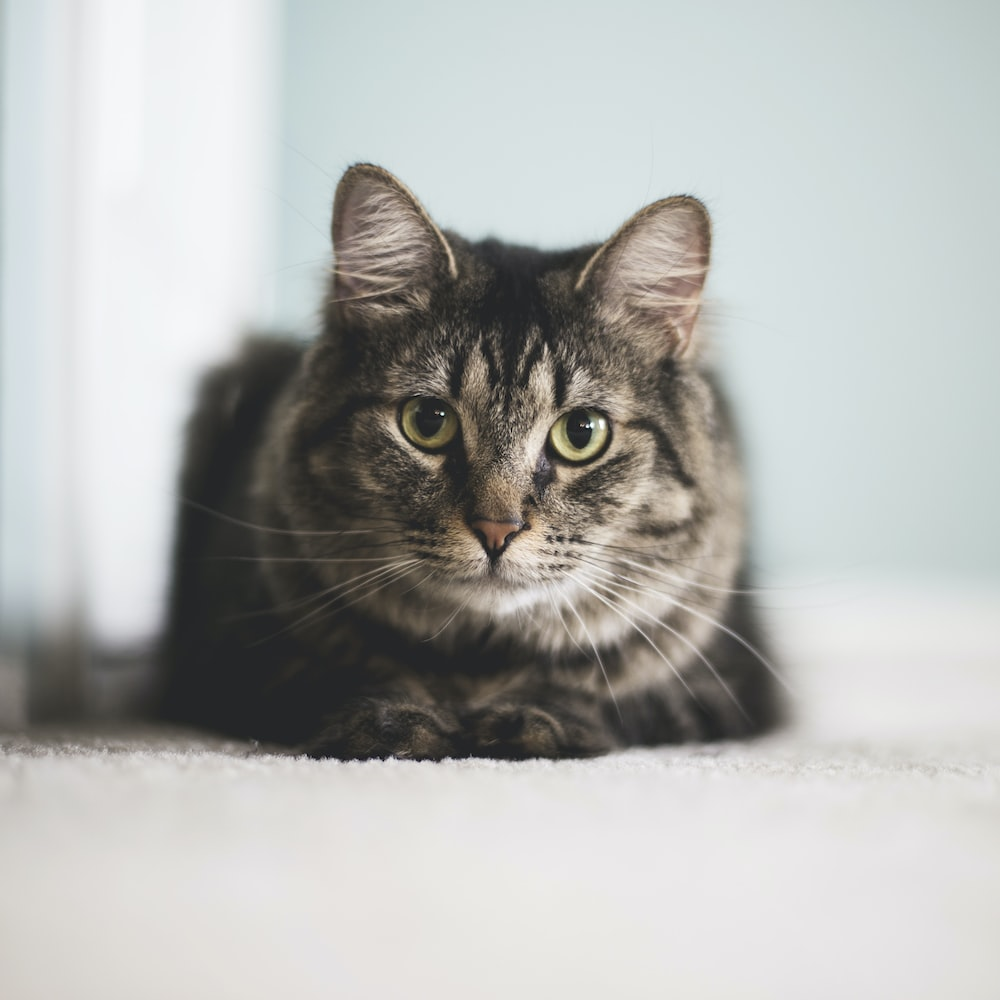
\includegraphics[width=1cm]{data/cat.jpeg}
			};

			\matrix[every node/.style={minimum height=0.15cm, minimum width=0.15cm, draw=black, fill=nodefill, inner sep=0pt}] at (1.65, 0.1) {
				\node{}; \& \node{}; \& \node{}; \& \node{}; \& \node{}; \& \node{}; \& \node{}; \& \node{};\\
				\node{}; \& \node{}; \& \node{}; \& \node{}; \& \node{}; \& \node{}; \& \node{}; \& \node{};\\
				\node{}; \& \node{}; \& \node{}; \& \node{}; \& \node{}; \& \node{}; \& \node{}; \& \node{};\\
				\node{}; \& \node{}; \& \node{}; \& \node{}; \& \node{}; \& \node{}; \& \node{}; \& \node{};\\
				\node{}; \& \node{}; \& \node{}; \& \node{}; \& \node{}; \& \node{}; \& \node{}; \& \node{};\\
				\node{}; \& \node{}; \& \node{}; \& \node{}; \& \node{}; \& \node{}; \& \node{}; \& \node{};\\
				\node{}; \& \node{}; \& \node{}; \& \node{}; \& \node{}; \& \node{}; \& \node{}; \& \node{};\\
				\node{}; \& \node{}; \& \node{}; \& \node{}; \& \node{}; \& \node{}; \& \node{}; \& \node{};\\
			};

			\matrix[every node/.style={minimum height=0.15cm, minimum width=0.15cm, draw=black, fill=nodefill, inner sep=0pt, outer sep=0pt}] (l1) at (1.75, 0) {
				\node{}; \& \node{}; \& \node{}; \& \node{}; \& \node{}; \& \node{}; \& \node{}; \& \node{};\\
				\node{}; \& \node{}; \& \node{}; \& \node{}; \& \node{}; \& \node{}; \& \node{}; \& \node{};\\
				\node{}; \& \node{}; \& \node{}; \& \node{}; \& \node{}; \& \node{}; \& \node{}; \& \node{};\\
				\node{}; \& \node{}; \& \node{}; \& \node{}; \& \node{}; \& \node{}; \& \node{}; \& \node{};\\
				\node{}; \& \node{}; \& \node{}; \& \node{}; \& \node{}; \& \node{}; \& \node{}; \& \node{};\\
				\node{}; \& \node{}; \& \node{}; \& \node{}; \& \node{}; \& \node{}; \& \node{}; \& \node{};\\
				\node{}; \& \node{}; \& \node{}; \& \node{}; \& \node{}; \& \node{}; \& \node{}; \& \node{};\\
				\node{}; \& \node{}; \& \node{}; \& \node{}; \& \node{}; \& \node{}; \& \node{}; \& \node{};\\
			};
			\draw[->] (l0) -- (l1);

			\matrix[every node/.style={minimum height=0.15cm, minimum width=0.15cm, draw=black, fill=nodefill, inner sep=0pt}] at (1.85, -0.1) {
				\node{}; \& \node{}; \& \node{}; \& \node{}; \& \node{}; \& \node{}; \& \node{}; \& \node{};\\
				\node{}; \& \node{}; \& \node{}; \& \node{}; \& \node{}; \& \node{}; \& \node{}; \& \node{};\\
				\node{}; \& \node{}; \& \node{}; \& \node{}; \& \node{}; \& \node{}; \& \node{}; \& \node{};\\
				\node{}; \& \node{}; \& \node{}; \& \node{}; \& \node{}; \& \node{}; \& \node{}; \& \node{};\\
				\node{}; \& \node{}; \& \node{}; \& \node{}; \& \node{}; \& \node{}; \& \node{}; \& \node{};\\
				\node{}; \& \node{}; \& \node{}; \& \node{}; \& \node{}; \& \node{}; \& \node{}; \& \node{};\\
				\node{}; \& \node{}; \& \node{}; \& \node{}; \& \node{}; \& \node{}; \& \node{}; \& \node{};\\
				\node{}; \& \node{}; \& \node{}; \& \node{}; \& \node{}; \& \node{}; \& \node{}; \& \node{};\\
			};

			\matrix[every node/.style={minimum height=0.15cm, minimum width=0.15cm, draw=black, fill=nodefill, inner sep=0pt}] at (3.4, 0.1) {
				\node{}; \& \node{}; \& \node{}; \& \node{}; \& \node{}; \& \node{};\\
				\node{}; \& \node{}; \& \node{}; \& \node{}; \& \node{}; \& \node{};\\
				\node{}; \& \node{}; \& \node{}; \& \node{}; \& \node{}; \& \node{};\\
				\node{}; \& \node{}; \& \node{}; \& \node{}; \& \node{}; \& \node{};\\
				\node{}; \& \node{}; \& \node{}; \& \node{}; \& \node{}; \& \node{};\\
				\node{}; \& \node{}; \& \node{}; \& \node{}; \& \node{}; \& \node{};\\
			};

			\matrix[every node/.style={minimum height=0.15cm, minimum width=0.15cm, draw=black, fill=nodefill, inner sep=0pt}] (l2)at (3.5, 0) {
				\node{}; \& \node{}; \& \node{}; \& \node{}; \& \node{}; \& \node{};\\
				\node{}; \& \node{}; \& \node{}; \& \node{}; \& \node{}; \& \node{};\\
				\node{}; \& \node{}; \& \node{}; \& \node{}; \& \node{}; \& \node{};\\
				\node{}; \& \node{}; \& \node{}; \& \node{}; \& \node{}; \& \node{};\\
				\node{}; \& \node{}; \& \node{}; \& \node{}; \& \node{}; \& \node{};\\
				\node{}; \& \node{}; \& \node{}; \& \node{}; \& \node{}; \& \node{};\\
			};
			\draw[->] (l1) -- (l2);

			\matrix[every node/.style={minimum height=0.15cm, minimum width=0.15cm, draw=black, fill=nodefill, inner sep=0pt}] at (3.6, -0.1) {
				\node{}; \& \node{}; \& \node{}; \& \node{}; \& \node{}; \& \node{};\\
				\node{}; \& \node{}; \& \node{}; \& \node{}; \& \node{}; \& \node{};\\
				\node{}; \& \node{}; \& \node{}; \& \node{}; \& \node{}; \& \node{};\\
				\node{}; \& \node{}; \& \node{}; \& \node{}; \& \node{}; \& \node{};\\
				\node{}; \& \node{}; \& \node{}; \& \node{}; \& \node{}; \& \node{};\\
				\node{}; \& \node{}; \& \node{}; \& \node{}; \& \node{}; \& \node{};\\
			};

			\matrix[every node/.style={minimum height=0.15cm, minimum width=0.15cm, draw=black, fill=nodefill, inner sep=0pt}] at (5.05, 0.2) {
				\node{}; \& \node{}; \& \node{}; \& \node{}; \& \node{}; \& \node{};\\
				\node{}; \& \node{}; \& \node{}; \& \node{}; \& \node{}; \& \node{};\\
				\node{}; \& \node{}; \& \node{}; \& \node{}; \& \node{}; \& \node{};\\
				\node{}; \& \node{}; \& \node{}; \& \node{}; \& \node{}; \& \node{};\\
				\node{}; \& \node{}; \& \node{}; \& \node{}; \& \node{}; \& \node{};\\
				\node{}; \& \node{}; \& \node{}; \& \node{}; \& \node{}; \& \node{};\\
			};

			\matrix[every node/.style={minimum height=0.15cm, minimum width=0.15cm, draw=black, fill=nodefill, inner sep=0pt}] at (5.15, 0.1) {
				\node{}; \& \node{}; \& \node{}; \& \node{}; \& \node{}; \& \node{};\\
				\node{}; \& \node{}; \& \node{}; \& \node{}; \& \node{}; \& \node{};\\
				\node{}; \& \node{}; \& \node{}; \& \node{}; \& \node{}; \& \node{};\\
				\node{}; \& \node{}; \& \node{}; \& \node{}; \& \node{}; \& \node{};\\
				\node{}; \& \node{}; \& \node{}; \& \node{}; \& \node{}; \& \node{};\\
				\node{}; \& \node{}; \& \node{}; \& \node{}; \& \node{}; \& \node{};\\
			};

			\matrix[every node/.style={minimum height=0.15cm, minimum width=0.15cm, draw=black, fill=nodefill, inner sep=0pt}] (l3) at (5.25, 0) {
				\node{}; \& \node{}; \& \node{}; \& \node{}; \& \node{}; \& \node{};\\
				\node{}; \& \node{}; \& \node{}; \& \node{}; \& \node{}; \& \node{};\\
				\node{}; \& \node{}; \& \node{}; \& \node{}; \& \node{}; \& \node{};\\
				\node{}; \& \node{}; \& \node{}; \& \node{}; \& \node{}; \& \node{};\\
				\node{}; \& \node{}; \& \node{}; \& \node{}; \& \node{}; \& \node{};\\
				\node{}; \& \node{}; \& \node{}; \& \node{}; \& \node{}; \& \node{};\\
			};
			\draw[->] (l2) -- ($ (l3.west) - (0.1, 0) $);

			\matrix[every node/.style={minimum height=0.15cm, minimum width=0.15cm, draw=black, fill=nodefill, inner sep=0pt}] at (5.35, -0.1) {
				\node{}; \& \node{}; \& \node{}; \& \node{}; \& \node{}; \& \node{};\\
				\node{}; \& \node{}; \& \node{}; \& \node{}; \& \node{}; \& \node{};\\
				\node{}; \& \node{}; \& \node{}; \& \node{}; \& \node{}; \& \node{};\\
				\node{}; \& \node{}; \& \node{}; \& \node{}; \& \node{}; \& \node{};\\
				\node{}; \& \node{}; \& \node{}; \& \node{}; \& \node{}; \& \node{};\\
				\node{}; \& \node{}; \& \node{}; \& \node{}; \& \node{}; \& \node{};\\
			};

			\matrix[every node/.style={minimum height=0.15cm, minimum width=0.15cm, draw=black, fill=nodefill, inner sep=0pt}] at (5.45, -0.2) {
				\node{}; \& \node{}; \& \node{}; \& \node{}; \& \node{}; \& \node{};\\
				\node{}; \& \node{}; \& \node{}; \& \node{}; \& \node{}; \& \node{};\\
				\node{}; \& \node{}; \& \node{}; \& \node{}; \& \node{}; \& \node{};\\
				\node{}; \& \node{}; \& \node{}; \& \node{}; \& \node{}; \& \node{};\\
				\node{}; \& \node{}; \& \node{}; \& \node{}; \& \node{}; \& \node{};\\
				\node{}; \& \node{}; \& \node{}; \& \node{}; \& \node{}; \& \node{};\\
			};

			\matrix[every node/.style={minimum height=0.15cm, minimum width=0.15cm, draw=black, fill=nodefill, inner sep=0pt}] at (6.8, 0.2) {
				\node{}; \& \node{}; \& \node{}; \& \node{};\\
				\node{}; \& \node{}; \& \node{}; \& \node{};\\
				\node{}; \& \node{}; \& \node{}; \& \node{};\\
				\node{}; \& \node{}; \& \node{}; \& \node{};\\
			};

			\matrix[every node/.style={minimum height=0.15cm, minimum width=0.15cm, draw=black, fill=nodefill, inner sep=0pt}] at (6.9, 0.1) {
				\node{}; \& \node{}; \& \node{}; \& \node{};\\
				\node{}; \& \node{}; \& \node{}; \& \node{};\\
				\node{}; \& \node{}; \& \node{}; \& \node{};\\
				\node{}; \& \node{}; \& \node{}; \& \node{};\\
			};

			\matrix[every node/.style={minimum height=0.15cm, minimum width=0.15cm, draw=black, fill=nodefill, inner sep=0pt}] (l4) at (7, 0) {
				\node{}; \& \node{}; \& \node{}; \& \node{};\\
				\node{}; \& \node{}; \& \node{}; \& \node{};\\
				\node{}; \& \node{}; \& \node{}; \& \node{};\\
				\node{}; \& \node{}; \& \node{}; \& \node{};\\
			};
			\draw[->] ($ (l3.east) + (0.1, 0) $) -- ($ (l4.west) + (-0.1, 0) $);

			\matrix[every node/.style={minimum height=0.15cm, minimum width=0.15cm, draw=black, fill=nodefill, inner sep=0pt}] at (7.1, -0.1) {
				\node{}; \& \node{}; \& \node{}; \& \node{};\\
				\node{}; \& \node{}; \& \node{}; \& \node{};\\
				\node{}; \& \node{}; \& \node{}; \& \node{};\\
				\node{}; \& \node{}; \& \node{}; \& \node{};\\
			};
			\matrix[every node/.style={minimum height=0.15cm, minimum width=0.15cm, draw=black, fill=nodefill, inner sep=0pt}] at (7.2, -0.2) {
				\node{}; \& \node{}; \& \node{}; \& \node{};\\
				\node{}; \& \node{}; \& \node{}; \& \node{};\\
				\node{}; \& \node{}; \& \node{}; \& \node{};\\
				\node{}; \& \node{}; \& \node{}; \& \node{};\\
			};

			\matrix[every node/.style={minimum height=0.15cm, minimum width=0.15cm, draw=black, fill=nodefill, inner sep=0pt}] at (8.25, 0.3) {
				\node{}; \& \node{}; \& \node{}; \& \node{};\\
				\node{}; \& \node{}; \& \node{}; \& \node{};\\
				\node{}; \& \node{}; \& \node{}; \& \node{};\\
				\node{}; \& \node{}; \& \node{}; \& \node{};\\
			};

			\matrix[every node/.style={minimum height=0.15cm, minimum width=0.15cm, draw=black, fill=nodefill, inner sep=0pt}] at (8.35, 0.2) {
				\node{}; \& \node{}; \& \node{}; \& \node{};\\
				\node{}; \& \node{}; \& \node{}; \& \node{};\\
				\node{}; \& \node{}; \& \node{}; \& \node{};\\
				\node{}; \& \node{}; \& \node{}; \& \node{};\\
			};

			\matrix[every node/.style={minimum height=0.15cm, minimum width=0.15cm, draw=black, fill=nodefill, inner sep=0pt}] at (8.45, 0.1) {
				\node{}; \& \node{}; \& \node{}; \& \node{};\\
				\node{}; \& \node{}; \& \node{}; \& \node{};\\
				\node{}; \& \node{}; \& \node{}; \& \node{};\\
				\node{}; \& \node{}; \& \node{}; \& \node{};\\
			};

			\matrix[every node/.style={minimum height=0.15cm, minimum width=0.15cm, draw=black, fill=nodefill, inner sep=0pt}] (l5) at (8.55, 0) {
				\node{}; \& \node{}; \& \node{}; \& \node{};\\
				\node{}; \& \node{}; \& \node{}; \& \node{};\\
				\node{}; \& \node{}; \& \node{}; \& \node{};\\
				\node{}; \& \node{}; \& \node{}; \& \node{};\\
			};
			\draw[->] ($ (l4.east) + (0.1, 0) $) -- ($ (l5.west) + (-0.2, 0) $);

			\matrix[every node/.style={minimum height=0.15cm, minimum width=0.15cm, draw=black, fill=nodefill, inner sep=0pt}] at (8.65, -0.1) {
				\node{}; \& \node{}; \& \node{}; \& \node{};\\
				\node{}; \& \node{}; \& \node{}; \& \node{};\\
				\node{}; \& \node{}; \& \node{}; \& \node{};\\
				\node{}; \& \node{}; \& \node{}; \& \node{};\\
			};

			\matrix[every node/.style={minimum height=0.15cm, minimum width=0.15cm, draw=black, fill=nodefill, inner sep=0pt}] at (8.75, -0.2) {
				\node{}; \& \node{}; \& \node{}; \& \node{};\\
				\node{}; \& \node{}; \& \node{}; \& \node{};\\
				\node{}; \& \node{}; \& \node{}; \& \node{};\\
				\node{}; \& \node{}; \& \node{}; \& \node{};\\
			};

			\matrix[every node/.style={minimum height=0.15cm, minimum width=0.15cm, draw=black, fill=nodefill, inner sep=0pt}] at (8.85, -0.3) {
				\node{}; \& \node{}; \& \node{}; \& \node{};\\
				\node{}; \& \node{}; \& \node{}; \& \node{};\\
				\node{}; \& \node{}; \& \node{}; \& \node{};\\
				\node{}; \& \node{}; \& \node{}; \& \node{};\\
			};


			\node[circle, draw=black, fill=nodefill, text depth=0, inner sep=2pt] (y1) at (10.5, 0.125) {\tiny{$y_0$}};
			\node[circle, draw=black, fill=nodefill, text depth=0, inner sep=2pt] (y2) at (10.75, -0.125) {\tiny{$y_1$}};

			\node[minimum height=0.15cm, minimum width=0.15cm, draw=black, fill=nodefill, inner sep=0pt] (n0) at (9.4, 0.3) {};
			\draw[->] (n0) -- (y1);
			\node[minimum height=0.15cm, minimum width=0.15cm, draw=black, fill=nodefill, inner sep=0pt] (n1) at (9.5, 0.2) {};
			\draw[->] (n1) -- (y1);
			\node[minimum height=0.15cm, minimum width=0.15cm, draw=black, fill=nodefill, inner sep=0pt] (n2) at (9.6, 0.1) {};
			\draw[->] (n2) -- (y1);
			\node[minimum height=0.15cm, minimum width=0.15cm, draw=black, fill=nodefill, inner sep=0pt] (n3) at (9.7, 0) {};
			\draw[->] ($ (l5.east) + (0.2, 0) $) -- ($ (n3.west) + (-0.15, 0) $);
			\draw[->] (n3) -- (y1);
			\node[minimum height=0.15cm, minimum width=0.15cm, draw=black, fill=nodefill, inner sep=0pt] (n4) at (9.8, -0.1) {};
			\draw[->] (n4) -- (y1);
			\node[minimum height=0.15cm, minimum width=0.15cm, draw=black, fill=nodefill, inner sep=0pt] (n5) at (9.9, -0.2) {};
			\draw[->] (n5) -- (y1);
			\node[minimum height=0.15cm, minimum width=0.15cm, draw=black, fill=nodefill, inner sep=0pt] (n6) at (10, -0.3) {};
			\draw[->] (n6) -- (y1);

			\node[minimum height=0.15cm, minimum width=0.15cm, draw=black, fill=nodefill, inner sep=0pt] (n0) at (9.4, 0.3) {};
			\draw[->] (n0) -- (y2);
			\node[minimum height=0.15cm, minimum width=0.15cm, draw=black, fill=nodefill, inner sep=0pt] (n1) at (9.5, 0.2) {};
			\draw[->] (n1) -- (y2);
			\node[minimum height=0.15cm, minimum width=0.15cm, draw=black, fill=nodefill, inner sep=0pt] (n2) at (9.6, 0.1) {};
			\draw[->] (n2) -- (y2);
			\node[minimum height=0.15cm, minimum width=0.15cm, draw=black, fill=nodefill, inner sep=0pt] (n3) at (9.7, 0) {};
			\draw[->] (n3) -- (y2);
			\node[minimum height=0.15cm, minimum width=0.15cm, draw=black, fill=nodefill, inner sep=0pt] (n4) at (9.8, -0.1) {};
			\draw[->] (n4) -- (y2);
			\node[minimum height=0.15cm, minimum width=0.15cm, draw=black, fill=nodefill, inner sep=0pt] (n5) at (9.9, -0.2) {};
			\draw[->] (n5) -- (y2);
			\node[minimum height=0.15cm, minimum width=0.15cm, draw=black, fill=nodefill, inner sep=0pt] (n6) at (10, -0.3) {};
			\draw[->] (n6) -- (y2);

			\node[] at (1.75, -2) {
				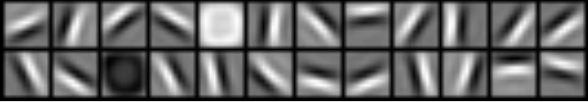
\includegraphics[width=3cm]{data/early.png}
			};

			\node[] at (5.25, -2) {
				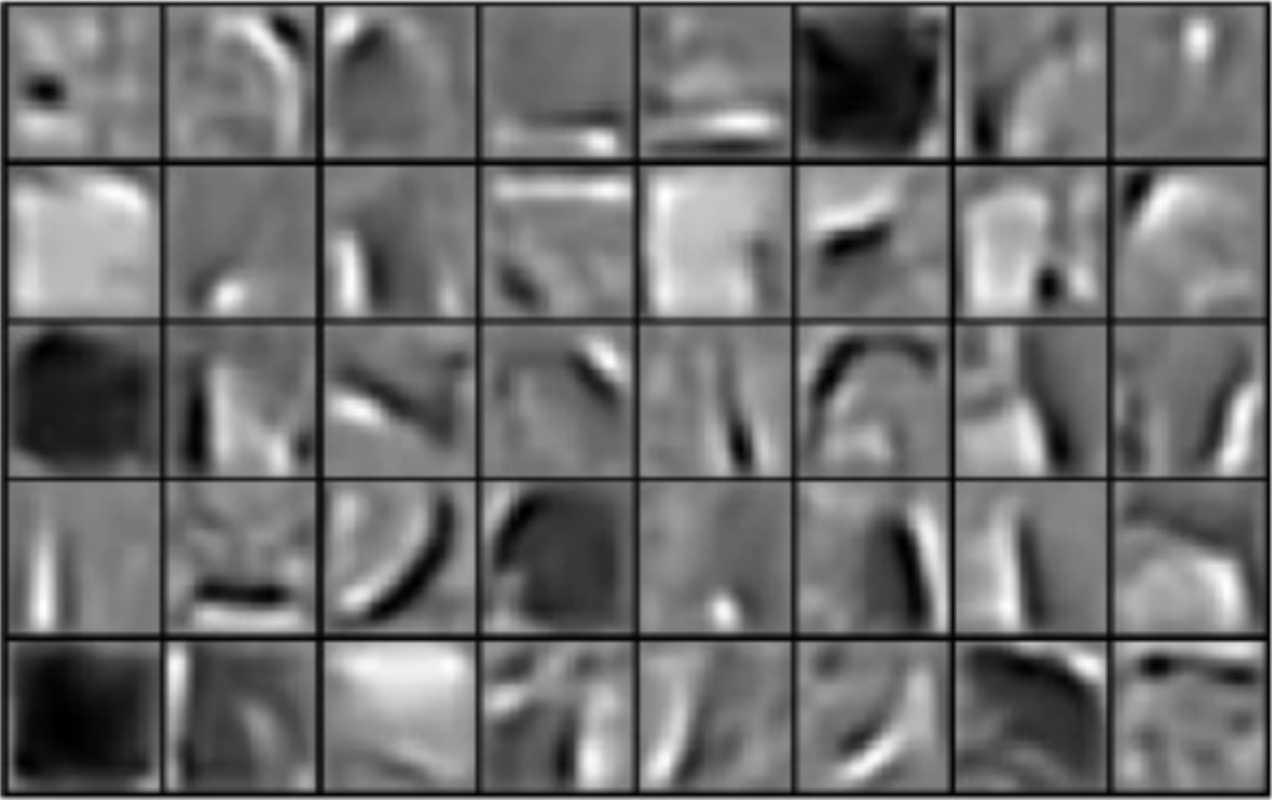
\includegraphics[width=3cm]{data/intermediate.png}
			};

			\node[] at (8.55, -2) {
				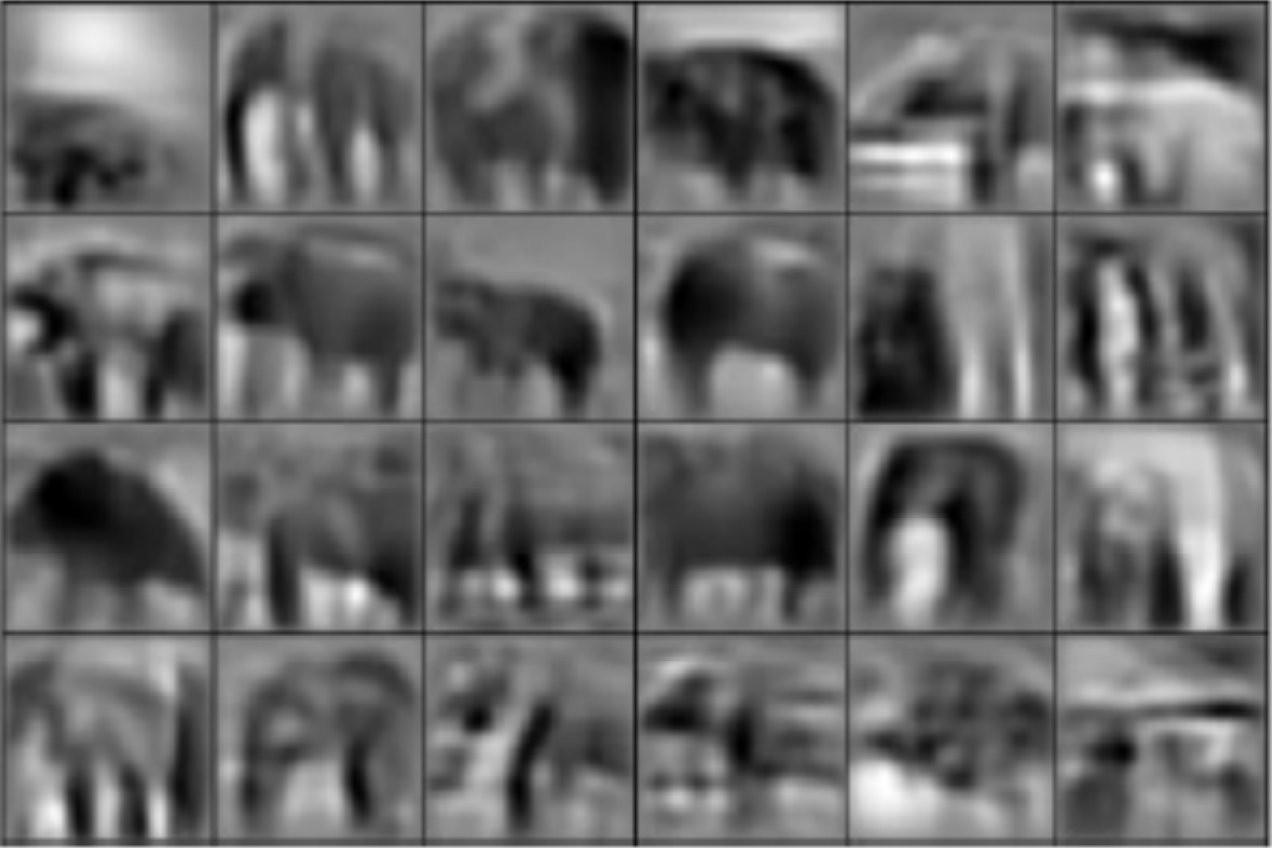
\includegraphics[width=3cm]{data/final.png}
			};

			\node[] at (6, 3) {};
			\node[] at (11, -3) {};

		\end{tikzpicture}
		}
		\vfill
	\end{frame}

	\begin{frame}{Bildegjenkjenning: Konvolusjonelle nevrale nettverk} % Cat again
		\centering
		\vfill
		\resizebox{\textwidth}{!}{

		\colorlet{nodefill}{cyan!40}
		\begin{tikzpicture}[
			ampersand replacement=\&
		]
			\node[inner sep=0pt, draw=black] (l0) at (0, 0) {
				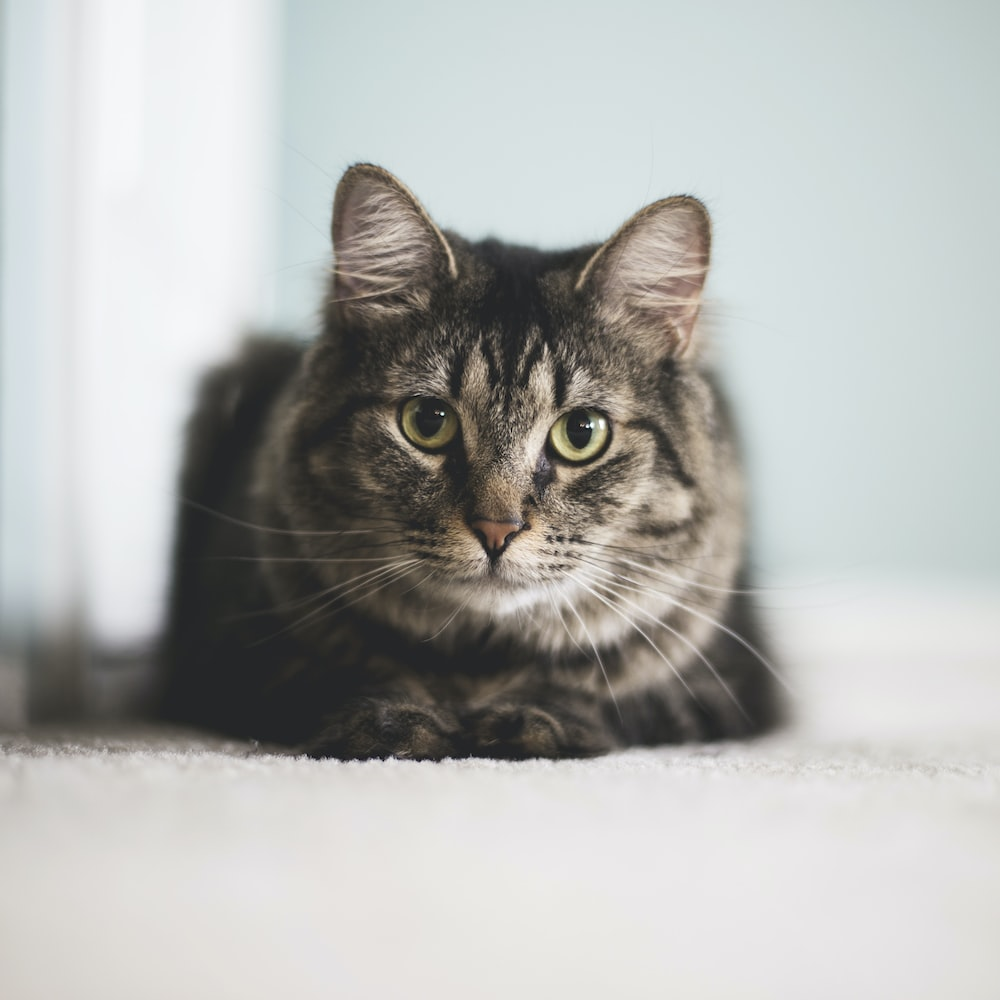
\includegraphics[width=1cm]{data/cat.jpeg}
			};

			\matrix[every node/.style={minimum height=0.15cm, minimum width=0.15cm, draw=black, fill=nodefill, inner sep=0pt}] at (1.65, 0.1) {
				\node{}; \& \node{}; \& \node{}; \& \node{}; \& \node{}; \& \node{}; \& \node{}; \& \node{};\\
				\node{}; \& \node{}; \& \node{}; \& \node{}; \& \node{}; \& \node{}; \& \node{}; \& \node{};\\
				\node{}; \& \node{}; \& \node{}; \& \node{}; \& \node{}; \& \node{}; \& \node{}; \& \node{};\\
				\node{}; \& \node{}; \& \node{}; \& \node{}; \& \node{}; \& \node{}; \& \node{}; \& \node{};\\
				\node{}; \& \node{}; \& \node{}; \& \node{}; \& \node{}; \& \node{}; \& \node{}; \& \node{};\\
				\node{}; \& \node{}; \& \node{}; \& \node{}; \& \node{}; \& \node{}; \& \node{}; \& \node{};\\
				\node{}; \& \node{}; \& \node{}; \& \node{}; \& \node{}; \& \node{}; \& \node{}; \& \node{};\\
				\node{}; \& \node{}; \& \node{}; \& \node{}; \& \node{}; \& \node{}; \& \node{}; \& \node{};\\
			};

			\matrix[every node/.style={minimum height=0.15cm, minimum width=0.15cm, draw=black, fill=nodefill, inner sep=0pt, outer sep=0pt}] (l1) at (1.75, 0) {
				\node{}; \& \node{}; \& \node{}; \& \node{}; \& \node{}; \& \node{}; \& \node{}; \& \node{};\\
				\node{}; \& \node{}; \& \node{}; \& \node{}; \& \node{}; \& \node{}; \& \node{}; \& \node{};\\
				\node{}; \& \node{}; \& \node{}; \& \node{}; \& \node{}; \& \node{}; \& \node{}; \& \node{};\\
				\node{}; \& \node{}; \& \node{}; \& \node{}; \& \node{}; \& \node{}; \& \node{}; \& \node{};\\
				\node{}; \& \node{}; \& \node{}; \& \node{}; \& \node{}; \& \node{}; \& \node{}; \& \node{};\\
				\node{}; \& \node{}; \& \node{}; \& \node{}; \& \node{}; \& \node{}; \& \node{}; \& \node{};\\
				\node{}; \& \node{}; \& \node{}; \& \node{}; \& \node{}; \& \node{}; \& \node{}; \& \node{};\\
				\node{}; \& \node{}; \& \node{}; \& \node{}; \& \node{}; \& \node{}; \& \node{}; \& \node{};\\
			};
			\draw[->] (l0) -- (l1);

			\matrix[every node/.style={minimum height=0.15cm, minimum width=0.15cm, draw=black, fill=nodefill, inner sep=0pt}] at (1.85, -0.1) {
				\node{}; \& \node{}; \& \node{}; \& \node{}; \& \node{}; \& \node{}; \& \node{}; \& \node{};\\
				\node{}; \& \node{}; \& \node{}; \& \node{}; \& \node{}; \& \node{}; \& \node{}; \& \node{};\\
				\node{}; \& \node{}; \& \node{}; \& \node{}; \& \node{}; \& \node{}; \& \node{}; \& \node{};\\
				\node{}; \& \node{}; \& \node{}; \& \node{}; \& \node{}; \& \node{}; \& \node{}; \& \node{};\\
				\node{}; \& \node{}; \& \node{}; \& \node{}; \& \node{}; \& \node{}; \& \node{}; \& \node{};\\
				\node{}; \& \node{}; \& \node{}; \& \node{}; \& \node{}; \& \node{}; \& \node{}; \& \node{};\\
				\node{}; \& \node{}; \& \node{}; \& \node{}; \& \node{}; \& \node{}; \& \node{}; \& \node{};\\
				\node{}; \& \node{}; \& \node{}; \& \node{}; \& \node{}; \& \node{}; \& \node{}; \& \node{};\\
			};

			\matrix[every node/.style={minimum height=0.15cm, minimum width=0.15cm, draw=black, fill=nodefill, inner sep=0pt}] at (3.4, 0.1) {
				\node{}; \& \node{}; \& \node{}; \& \node{}; \& \node{}; \& \node{};\\
				\node{}; \& \node{}; \& \node{}; \& \node{}; \& \node{}; \& \node{};\\
				\node{}; \& \node{}; \& \node{}; \& \node{}; \& \node{}; \& \node{};\\
				\node{}; \& \node{}; \& \node{}; \& \node{}; \& \node{}; \& \node{};\\
				\node{}; \& \node{}; \& \node{}; \& \node{}; \& \node{}; \& \node{};\\
				\node{}; \& \node{}; \& \node{}; \& \node{}; \& \node{}; \& \node{};\\
			};

			\matrix[every node/.style={minimum height=0.15cm, minimum width=0.15cm, draw=black, fill=nodefill, inner sep=0pt}] (l2)at (3.5, 0) {
				\node{}; \& \node{}; \& \node{}; \& \node{}; \& \node{}; \& \node{};\\
				\node{}; \& \node{}; \& \node{}; \& \node{}; \& \node{}; \& \node{};\\
				\node{}; \& \node{}; \& \node{}; \& \node{}; \& \node{}; \& \node{};\\
				\node{}; \& \node{}; \& \node{}; \& \node{}; \& \node{}; \& \node{};\\
				\node{}; \& \node{}; \& \node{}; \& \node{}; \& \node{}; \& \node{};\\
				\node{}; \& \node{}; \& \node{}; \& \node{}; \& \node{}; \& \node{};\\
			};
			\draw[->] (l1) -- (l2);

			\matrix[every node/.style={minimum height=0.15cm, minimum width=0.15cm, draw=black, fill=nodefill, inner sep=0pt}] at (3.6, -0.1) {
				\node{}; \& \node{}; \& \node{}; \& \node{}; \& \node{}; \& \node{};\\
				\node{}; \& \node{}; \& \node{}; \& \node{}; \& \node{}; \& \node{};\\
				\node{}; \& \node{}; \& \node{}; \& \node{}; \& \node{}; \& \node{};\\
				\node{}; \& \node{}; \& \node{}; \& \node{}; \& \node{}; \& \node{};\\
				\node{}; \& \node{}; \& \node{}; \& \node{}; \& \node{}; \& \node{};\\
				\node{}; \& \node{}; \& \node{}; \& \node{}; \& \node{}; \& \node{};\\
			};

			\matrix[every node/.style={minimum height=0.15cm, minimum width=0.15cm, draw=black, fill=nodefill, inner sep=0pt}] at (5.05, 0.2) {
				\node{}; \& \node{}; \& \node{}; \& \node{}; \& \node{}; \& \node{};\\
				\node{}; \& \node{}; \& \node{}; \& \node{}; \& \node{}; \& \node{};\\
				\node{}; \& \node{}; \& \node{}; \& \node{}; \& \node{}; \& \node{};\\
				\node{}; \& \node{}; \& \node{}; \& \node{}; \& \node{}; \& \node{};\\
				\node{}; \& \node{}; \& \node{}; \& \node{}; \& \node{}; \& \node{};\\
				\node{}; \& \node{}; \& \node{}; \& \node{}; \& \node{}; \& \node{};\\
			};

			\matrix[every node/.style={minimum height=0.15cm, minimum width=0.15cm, draw=black, fill=nodefill, inner sep=0pt}] at (5.15, 0.1) {
				\node{}; \& \node{}; \& \node{}; \& \node{}; \& \node{}; \& \node{};\\
				\node{}; \& \node{}; \& \node{}; \& \node{}; \& \node{}; \& \node{};\\
				\node{}; \& \node{}; \& \node{}; \& \node{}; \& \node{}; \& \node{};\\
				\node{}; \& \node{}; \& \node{}; \& \node{}; \& \node{}; \& \node{};\\
				\node{}; \& \node{}; \& \node{}; \& \node{}; \& \node{}; \& \node{};\\
				\node{}; \& \node{}; \& \node{}; \& \node{}; \& \node{}; \& \node{};\\
			};

			\matrix[every node/.style={minimum height=0.15cm, minimum width=0.15cm, draw=black, fill=nodefill, inner sep=0pt}] (l3) at (5.25, 0) {
				\node{}; \& \node{}; \& \node{}; \& \node{}; \& \node{}; \& \node{};\\
				\node{}; \& \node{}; \& \node{}; \& \node{}; \& \node{}; \& \node{};\\
				\node{}; \& \node{}; \& \node{}; \& \node{}; \& \node{}; \& \node{};\\
				\node{}; \& \node{}; \& \node{}; \& \node{}; \& \node{}; \& \node{};\\
				\node{}; \& \node{}; \& \node{}; \& \node{}; \& \node{}; \& \node{};\\
				\node{}; \& \node{}; \& \node{}; \& \node{}; \& \node{}; \& \node{};\\
			};
			\draw[->] (l2) -- ($ (l3.west) - (0.1, 0) $);

			\matrix[every node/.style={minimum height=0.15cm, minimum width=0.15cm, draw=black, fill=nodefill, inner sep=0pt}] at (5.35, -0.1) {
				\node{}; \& \node{}; \& \node{}; \& \node{}; \& \node{}; \& \node{};\\
				\node{}; \& \node{}; \& \node{}; \& \node{}; \& \node{}; \& \node{};\\
				\node{}; \& \node{}; \& \node{}; \& \node{}; \& \node{}; \& \node{};\\
				\node{}; \& \node{}; \& \node{}; \& \node{}; \& \node{}; \& \node{};\\
				\node{}; \& \node{}; \& \node{}; \& \node{}; \& \node{}; \& \node{};\\
				\node{}; \& \node{}; \& \node{}; \& \node{}; \& \node{}; \& \node{};\\
			};

			\matrix[every node/.style={minimum height=0.15cm, minimum width=0.15cm, draw=black, fill=nodefill, inner sep=0pt}] at (5.45, -0.2) {
				\node{}; \& \node{}; \& \node{}; \& \node{}; \& \node{}; \& \node{};\\
				\node{}; \& \node{}; \& \node{}; \& \node{}; \& \node{}; \& \node{};\\
				\node{}; \& \node{}; \& \node{}; \& \node{}; \& \node{}; \& \node{};\\
				\node{}; \& \node{}; \& \node{}; \& \node{}; \& \node{}; \& \node{};\\
				\node{}; \& \node{}; \& \node{}; \& \node{}; \& \node{}; \& \node{};\\
				\node{}; \& \node{}; \& \node{}; \& \node{}; \& \node{}; \& \node{};\\
			};

			\matrix[every node/.style={minimum height=0.15cm, minimum width=0.15cm, draw=black, fill=nodefill, inner sep=0pt}] at (6.8, 0.2) {
				\node{}; \& \node{}; \& \node{}; \& \node{};\\
				\node{}; \& \node{}; \& \node{}; \& \node{};\\
				\node{}; \& \node{}; \& \node{}; \& \node{};\\
				\node{}; \& \node{}; \& \node{}; \& \node{};\\
			};

			\matrix[every node/.style={minimum height=0.15cm, minimum width=0.15cm, draw=black, fill=nodefill, inner sep=0pt}] at (6.9, 0.1) {
				\node{}; \& \node{}; \& \node{}; \& \node{};\\
				\node{}; \& \node{}; \& \node{}; \& \node{};\\
				\node{}; \& \node{}; \& \node{}; \& \node{};\\
				\node{}; \& \node{}; \& \node{}; \& \node{};\\
			};

			\matrix[every node/.style={minimum height=0.15cm, minimum width=0.15cm, draw=black, fill=nodefill, inner sep=0pt}] (l4) at (7, 0) {
				\node{}; \& \node{}; \& \node{}; \& \node{};\\
				\node{}; \& \node{}; \& \node{}; \& \node{};\\
				\node{}; \& \node{}; \& \node{}; \& \node{};\\
				\node{}; \& \node{}; \& \node{}; \& \node{};\\
			};
			\draw[->] ($ (l3.east) + (0.1, 0) $) -- ($ (l4.west) + (-0.1, 0) $);

			\matrix[every node/.style={minimum height=0.15cm, minimum width=0.15cm, draw=black, fill=nodefill, inner sep=0pt}] at (7.1, -0.1) {
				\node{}; \& \node{}; \& \node{}; \& \node{};\\
				\node{}; \& \node{}; \& \node{}; \& \node{};\\
				\node{}; \& \node{}; \& \node{}; \& \node{};\\
				\node{}; \& \node{}; \& \node{}; \& \node{};\\
			};
			\matrix[every node/.style={minimum height=0.15cm, minimum width=0.15cm, draw=black, fill=nodefill, inner sep=0pt}] at (7.2, -0.2) {
				\node{}; \& \node{}; \& \node{}; \& \node{};\\
				\node{}; \& \node{}; \& \node{}; \& \node{};\\
				\node{}; \& \node{}; \& \node{}; \& \node{};\\
				\node{}; \& \node{}; \& \node{}; \& \node{};\\
			};

			\matrix[every node/.style={minimum height=0.15cm, minimum width=0.15cm, draw=black, fill=nodefill, inner sep=0pt}] at (8.25, 0.3) {
				\node{}; \& \node{}; \& \node{}; \& \node{};\\
				\node{}; \& \node{}; \& \node{}; \& \node{};\\
				\node{}; \& \node{}; \& \node{}; \& \node{};\\
				\node{}; \& \node{}; \& \node{}; \& \node{};\\
			};

			\matrix[every node/.style={minimum height=0.15cm, minimum width=0.15cm, draw=black, fill=nodefill, inner sep=0pt}] at (8.35, 0.2) {
				\node{}; \& \node{}; \& \node{}; \& \node{};\\
				\node{}; \& \node{}; \& \node{}; \& \node{};\\
				\node{}; \& \node{}; \& \node{}; \& \node{};\\
				\node{}; \& \node{}; \& \node{}; \& \node{};\\
			};

			\matrix[every node/.style={minimum height=0.15cm, minimum width=0.15cm, draw=black, fill=nodefill, inner sep=0pt}] at (8.45, 0.1) {
				\node{}; \& \node{}; \& \node{}; \& \node{};\\
				\node{}; \& \node{}; \& \node{}; \& \node{};\\
				\node{}; \& \node{}; \& \node{}; \& \node{};\\
				\node{}; \& \node{}; \& \node{}; \& \node{};\\
			};

			\matrix[every node/.style={minimum height=0.15cm, minimum width=0.15cm, draw=black, fill=nodefill, inner sep=0pt}] (l5) at (8.55, 0) {
				\node{}; \& \node{}; \& \node{}; \& \node{};\\
				\node{}; \& \node{}; \& \node{}; \& \node{};\\
				\node{}; \& \node{}; \& \node{}; \& \node{};\\
				\node{}; \& \node{}; \& \node{}; \& \node{};\\
			};
			\draw[->] ($ (l4.east) + (0.1, 0) $) -- ($ (l5.west) + (-0.2, 0) $);

			\matrix[every node/.style={minimum height=0.15cm, minimum width=0.15cm, draw=black, fill=nodefill, inner sep=0pt}] at (8.65, -0.1) {
				\node{}; \& \node{}; \& \node{}; \& \node{};\\
				\node{}; \& \node{}; \& \node{}; \& \node{};\\
				\node{}; \& \node{}; \& \node{}; \& \node{};\\
				\node{}; \& \node{}; \& \node{}; \& \node{};\\
			};

			\matrix[every node/.style={minimum height=0.15cm, minimum width=0.15cm, draw=black, fill=nodefill, inner sep=0pt}] at (8.75, -0.2) {
				\node{}; \& \node{}; \& \node{}; \& \node{};\\
				\node{}; \& \node{}; \& \node{}; \& \node{};\\
				\node{}; \& \node{}; \& \node{}; \& \node{};\\
				\node{}; \& \node{}; \& \node{}; \& \node{};\\
			};

			\matrix[every node/.style={minimum height=0.15cm, minimum width=0.15cm, draw=black, fill=nodefill, inner sep=0pt}] at (8.85, -0.3) {
				\node{}; \& \node{}; \& \node{}; \& \node{};\\
				\node{}; \& \node{}; \& \node{}; \& \node{};\\
				\node{}; \& \node{}; \& \node{}; \& \node{};\\
				\node{}; \& \node{}; \& \node{}; \& \node{};\\
			};


			\node[circle, draw=black, fill=nodefill, text depth=0, inner sep=2pt] (y1) at (10.5, 0.125) {\tiny{$y_0$}};
			\node[circle, draw=black, fill=nodefill, text depth=0, inner sep=2pt] (y2) at (10.75, -0.125) {\tiny{$y_1$}};

			\node[minimum height=0.15cm, minimum width=0.15cm, draw=black, fill=nodefill, inner sep=0pt] (n0) at (9.4, 0.3) {};
			\draw[->] (n0) -- (y1);
			\node[minimum height=0.15cm, minimum width=0.15cm, draw=black, fill=nodefill, inner sep=0pt] (n1) at (9.5, 0.2) {};
			\draw[->] (n1) -- (y1);
			\node[minimum height=0.15cm, minimum width=0.15cm, draw=black, fill=nodefill, inner sep=0pt] (n2) at (9.6, 0.1) {};
			\draw[->] (n2) -- (y1);
			\node[minimum height=0.15cm, minimum width=0.15cm, draw=black, fill=nodefill, inner sep=0pt] (n3) at (9.7, 0) {};
			\draw[->] ($ (l5.east) + (0.2, 0) $) -- ($ (n3.west) + (-0.15, 0) $);
			\draw[->] (n3) -- (y1);
			\node[minimum height=0.15cm, minimum width=0.15cm, draw=black, fill=nodefill, inner sep=0pt] (n4) at (9.8, -0.1) {};
			\draw[->] (n4) -- (y1);
			\node[minimum height=0.15cm, minimum width=0.15cm, draw=black, fill=nodefill, inner sep=0pt] (n5) at (9.9, -0.2) {};
			\draw[->] (n5) -- (y1);
			\node[minimum height=0.15cm, minimum width=0.15cm, draw=black, fill=nodefill, inner sep=0pt] (n6) at (10, -0.3) {};
			\draw[->] (n6) -- (y1);

			\node[minimum height=0.15cm, minimum width=0.15cm, draw=black, fill=nodefill, inner sep=0pt] (n0) at (9.4, 0.3) {};
			\draw[->] (n0) -- (y2);
			\node[minimum height=0.15cm, minimum width=0.15cm, draw=black, fill=nodefill, inner sep=0pt] (n1) at (9.5, 0.2) {};
			\draw[->] (n1) -- (y2);
			\node[minimum height=0.15cm, minimum width=0.15cm, draw=black, fill=nodefill, inner sep=0pt] (n2) at (9.6, 0.1) {};
			\draw[->] (n2) -- (y2);
			\node[minimum height=0.15cm, minimum width=0.15cm, draw=black, fill=nodefill, inner sep=0pt] (n3) at (9.7, 0) {};
			\draw[->] (n3) -- (y2);
			\node[minimum height=0.15cm, minimum width=0.15cm, draw=black, fill=nodefill, inner sep=0pt] (n4) at (9.8, -0.1) {};
			\draw[->] (n4) -- (y2);
			\node[minimum height=0.15cm, minimum width=0.15cm, draw=black, fill=nodefill, inner sep=0pt] (n5) at (9.9, -0.2) {};
			\draw[->] (n5) -- (y2);
			\node[minimum height=0.15cm, minimum width=0.15cm, draw=black, fill=nodefill, inner sep=0pt] (n6) at (10, -0.3) {};
			\draw[->] (n6) -- (y2);

			\node[] at (6, 3) {};
			\node[] at (11, -3) {};

		\end{tikzpicture}
		}
		\vfill
	\end{frame}

	\begin{frame}{Bildegjenkjenning: Konvolusjonelle nevrale nettverk} % Bottleneck
		\centering
		\vfill
		\resizebox{\textwidth}{!}{

		\colorlet{nodefill}{cyan!40}
		\begin{tikzpicture}[
			ampersand replacement=\&
		]
			\node[inner sep=0pt, draw=black] (l0) at (0, 0) {
				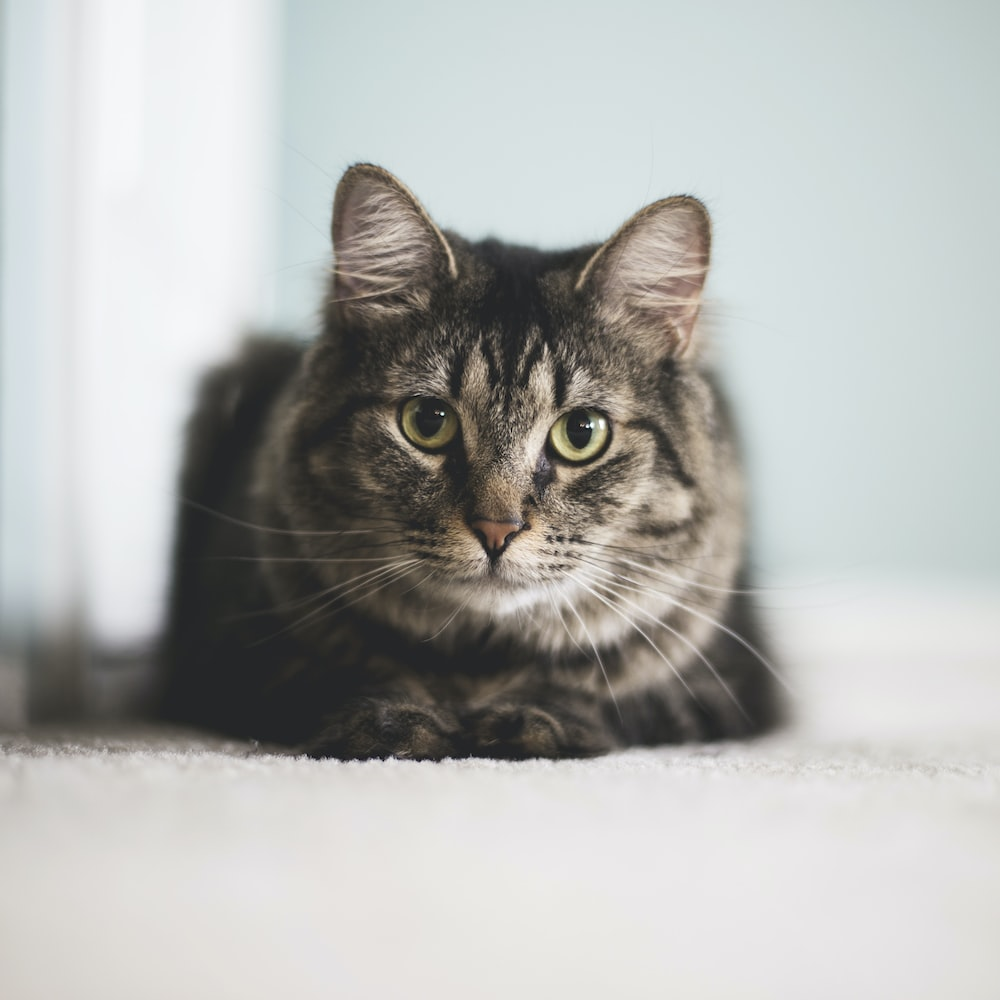
\includegraphics[width=1cm]{data/cat.jpeg}
			};

			\matrix[every node/.style={minimum height=0.15cm, minimum width=0.15cm, draw=black, fill=nodefill, inner sep=0pt}] at (1.65, 0.1) {
				\node{}; \& \node{}; \& \node{}; \& \node{}; \& \node{}; \& \node{}; \& \node{}; \& \node{};\\
				\node{}; \& \node{}; \& \node{}; \& \node{}; \& \node{}; \& \node{}; \& \node{}; \& \node{};\\
				\node{}; \& \node{}; \& \node{}; \& \node{}; \& \node{}; \& \node{}; \& \node{}; \& \node{};\\
				\node{}; \& \node{}; \& \node{}; \& \node{}; \& \node{}; \& \node{}; \& \node{}; \& \node{};\\
				\node{}; \& \node{}; \& \node{}; \& \node{}; \& \node{}; \& \node{}; \& \node{}; \& \node{};\\
				\node{}; \& \node{}; \& \node{}; \& \node{}; \& \node{}; \& \node{}; \& \node{}; \& \node{};\\
				\node{}; \& \node{}; \& \node{}; \& \node{}; \& \node{}; \& \node{}; \& \node{}; \& \node{};\\
				\node{}; \& \node{}; \& \node{}; \& \node{}; \& \node{}; \& \node{}; \& \node{}; \& \node{};\\
			};

			\matrix[every node/.style={minimum height=0.15cm, minimum width=0.15cm, draw=black, fill=nodefill, inner sep=0pt, outer sep=0pt}] (l1) at (1.75, 0) {
				\node{}; \& \node{}; \& \node{}; \& \node{}; \& \node{}; \& \node{}; \& \node{}; \& \node{};\\
				\node{}; \& \node{}; \& \node{}; \& \node{}; \& \node{}; \& \node{}; \& \node{}; \& \node{};\\
				\node{}; \& \node{}; \& \node{}; \& \node{}; \& \node{}; \& \node{}; \& \node{}; \& \node{};\\
				\node{}; \& \node{}; \& \node{}; \& \node{}; \& \node{}; \& \node{}; \& \node{}; \& \node{};\\
				\node{}; \& \node{}; \& \node{}; \& \node{}; \& \node{}; \& \node{}; \& \node{}; \& \node{};\\
				\node{}; \& \node{}; \& \node{}; \& \node{}; \& \node{}; \& \node{}; \& \node{}; \& \node{};\\
				\node{}; \& \node{}; \& \node{}; \& \node{}; \& \node{}; \& \node{}; \& \node{}; \& \node{};\\
				\node{}; \& \node{}; \& \node{}; \& \node{}; \& \node{}; \& \node{}; \& \node{}; \& \node{};\\
			};
			\draw[->] (l0) -- (l1);

			\matrix[every node/.style={minimum height=0.15cm, minimum width=0.15cm, draw=black, fill=nodefill, inner sep=0pt}] at (1.85, -0.1) {
				\node{}; \& \node{}; \& \node{}; \& \node{}; \& \node{}; \& \node{}; \& \node{}; \& \node{};\\
				\node{}; \& \node{}; \& \node{}; \& \node{}; \& \node{}; \& \node{}; \& \node{}; \& \node{};\\
				\node{}; \& \node{}; \& \node{}; \& \node{}; \& \node{}; \& \node{}; \& \node{}; \& \node{};\\
				\node{}; \& \node{}; \& \node{}; \& \node{}; \& \node{}; \& \node{}; \& \node{}; \& \node{};\\
				\node{}; \& \node{}; \& \node{}; \& \node{}; \& \node{}; \& \node{}; \& \node{}; \& \node{};\\
				\node{}; \& \node{}; \& \node{}; \& \node{}; \& \node{}; \& \node{}; \& \node{}; \& \node{};\\
				\node{}; \& \node{}; \& \node{}; \& \node{}; \& \node{}; \& \node{}; \& \node{}; \& \node{};\\
				\node{}; \& \node{}; \& \node{}; \& \node{}; \& \node{}; \& \node{}; \& \node{}; \& \node{};\\
			};

			\matrix[every node/.style={minimum height=0.15cm, minimum width=0.15cm, draw=black, fill=nodefill, inner sep=0pt}] at (3.4, 0.1) {
				\node{}; \& \node{}; \& \node{}; \& \node{}; \& \node{}; \& \node{};\\
				\node{}; \& \node{}; \& \node{}; \& \node{}; \& \node{}; \& \node{};\\
				\node{}; \& \node{}; \& \node{}; \& \node{}; \& \node{}; \& \node{};\\
				\node{}; \& \node{}; \& \node{}; \& \node{}; \& \node{}; \& \node{};\\
				\node{}; \& \node{}; \& \node{}; \& \node{}; \& \node{}; \& \node{};\\
				\node{}; \& \node{}; \& \node{}; \& \node{}; \& \node{}; \& \node{};\\
			};

			\matrix[every node/.style={minimum height=0.15cm, minimum width=0.15cm, draw=black, fill=nodefill, inner sep=0pt}] (l2)at (3.5, 0) {
				\node{}; \& \node{}; \& \node{}; \& \node{}; \& \node{}; \& \node{};\\
				\node{}; \& \node{}; \& \node{}; \& \node{}; \& \node{}; \& \node{};\\
				\node{}; \& \node{}; \& \node{}; \& \node{}; \& \node{}; \& \node{};\\
				\node{}; \& \node{}; \& \node{}; \& \node{}; \& \node{}; \& \node{};\\
				\node{}; \& \node{}; \& \node{}; \& \node{}; \& \node{}; \& \node{};\\
				\node{}; \& \node{}; \& \node{}; \& \node{}; \& \node{}; \& \node{};\\
			};
			\draw[->] (l1) -- (l2);

			\matrix[every node/.style={minimum height=0.15cm, minimum width=0.15cm, draw=black, fill=nodefill, inner sep=0pt}] at (3.6, -0.1) {
				\node{}; \& \node{}; \& \node{}; \& \node{}; \& \node{}; \& \node{};\\
				\node{}; \& \node{}; \& \node{}; \& \node{}; \& \node{}; \& \node{};\\
				\node{}; \& \node{}; \& \node{}; \& \node{}; \& \node{}; \& \node{};\\
				\node{}; \& \node{}; \& \node{}; \& \node{}; \& \node{}; \& \node{};\\
				\node{}; \& \node{}; \& \node{}; \& \node{}; \& \node{}; \& \node{};\\
				\node{}; \& \node{}; \& \node{}; \& \node{}; \& \node{}; \& \node{};\\
			};

			\matrix[every node/.style={minimum height=0.15cm, minimum width=0.15cm, draw=black, fill=nodefill, inner sep=0pt}] at (5.05, 0.2) {
				\node{}; \& \node{}; \& \node{}; \& \node{}; \& \node{}; \& \node{};\\
				\node{}; \& \node{}; \& \node{}; \& \node{}; \& \node{}; \& \node{};\\
				\node{}; \& \node{}; \& \node{}; \& \node{}; \& \node{}; \& \node{};\\
				\node{}; \& \node{}; \& \node{}; \& \node{}; \& \node{}; \& \node{};\\
				\node{}; \& \node{}; \& \node{}; \& \node{}; \& \node{}; \& \node{};\\
				\node{}; \& \node{}; \& \node{}; \& \node{}; \& \node{}; \& \node{};\\
			};

			\matrix[every node/.style={minimum height=0.15cm, minimum width=0.15cm, draw=black, fill=nodefill, inner sep=0pt}] at (5.15, 0.1) {
				\node{}; \& \node{}; \& \node{}; \& \node{}; \& \node{}; \& \node{};\\
				\node{}; \& \node{}; \& \node{}; \& \node{}; \& \node{}; \& \node{};\\
				\node{}; \& \node{}; \& \node{}; \& \node{}; \& \node{}; \& \node{};\\
				\node{}; \& \node{}; \& \node{}; \& \node{}; \& \node{}; \& \node{};\\
				\node{}; \& \node{}; \& \node{}; \& \node{}; \& \node{}; \& \node{};\\
				\node{}; \& \node{}; \& \node{}; \& \node{}; \& \node{}; \& \node{};\\
			};

			\matrix[every node/.style={minimum height=0.15cm, minimum width=0.15cm, draw=black, fill=nodefill, inner sep=0pt}] (l3) at (5.25, 0) {
				\node{}; \& \node{}; \& \node{}; \& \node{}; \& \node{}; \& \node{};\\
				\node{}; \& \node{}; \& \node{}; \& \node{}; \& \node{}; \& \node{};\\
				\node{}; \& \node{}; \& \node{}; \& \node{}; \& \node{}; \& \node{};\\
				\node{}; \& \node{}; \& \node{}; \& \node{}; \& \node{}; \& \node{};\\
				\node{}; \& \node{}; \& \node{}; \& \node{}; \& \node{}; \& \node{};\\
				\node{}; \& \node{}; \& \node{}; \& \node{}; \& \node{}; \& \node{};\\
			};
			\draw[->] (l2) -- ($ (l3.west) - (0.1, 0) $);

			\matrix[every node/.style={minimum height=0.15cm, minimum width=0.15cm, draw=black, fill=nodefill, inner sep=0pt}] at (5.35, -0.1) {
				\node{}; \& \node{}; \& \node{}; \& \node{}; \& \node{}; \& \node{};\\
				\node{}; \& \node{}; \& \node{}; \& \node{}; \& \node{}; \& \node{};\\
				\node{}; \& \node{}; \& \node{}; \& \node{}; \& \node{}; \& \node{};\\
				\node{}; \& \node{}; \& \node{}; \& \node{}; \& \node{}; \& \node{};\\
				\node{}; \& \node{}; \& \node{}; \& \node{}; \& \node{}; \& \node{};\\
				\node{}; \& \node{}; \& \node{}; \& \node{}; \& \node{}; \& \node{};\\
			};

			\matrix[every node/.style={minimum height=0.15cm, minimum width=0.15cm, draw=black, fill=nodefill, inner sep=0pt}] at (5.45, -0.2) {
				\node{}; \& \node{}; \& \node{}; \& \node{}; \& \node{}; \& \node{};\\
				\node{}; \& \node{}; \& \node{}; \& \node{}; \& \node{}; \& \node{};\\
				\node{}; \& \node{}; \& \node{}; \& \node{}; \& \node{}; \& \node{};\\
				\node{}; \& \node{}; \& \node{}; \& \node{}; \& \node{}; \& \node{};\\
				\node{}; \& \node{}; \& \node{}; \& \node{}; \& \node{}; \& \node{};\\
				\node{}; \& \node{}; \& \node{}; \& \node{}; \& \node{}; \& \node{};\\
			};

			\matrix[every node/.style={minimum height=0.15cm, minimum width=0.15cm, draw=black, fill=nodefill, inner sep=0pt}] at (6.8, 0.2) {
				\node{}; \& \node{}; \& \node{}; \& \node{};\\
				\node{}; \& \node{}; \& \node{}; \& \node{};\\
				\node{}; \& \node{}; \& \node{}; \& \node{};\\
				\node{}; \& \node{}; \& \node{}; \& \node{};\\
			};

			\matrix[every node/.style={minimum height=0.15cm, minimum width=0.15cm, draw=black, fill=nodefill, inner sep=0pt}] at (6.9, 0.1) {
				\node{}; \& \node{}; \& \node{}; \& \node{};\\
				\node{}; \& \node{}; \& \node{}; \& \node{};\\
				\node{}; \& \node{}; \& \node{}; \& \node{};\\
				\node{}; \& \node{}; \& \node{}; \& \node{};\\
			};

			\matrix[every node/.style={minimum height=0.15cm, minimum width=0.15cm, draw=black, fill=nodefill, inner sep=0pt}] (l4) at (7, 0) {
				\node{}; \& \node{}; \& \node{}; \& \node{};\\
				\node{}; \& \node{}; \& \node{}; \& \node{};\\
				\node{}; \& \node{}; \& \node{}; \& \node{};\\
				\node{}; \& \node{}; \& \node{}; \& \node{};\\
			};
			\draw[->] ($ (l3.east) + (0.1, 0) $) -- ($ (l4.west) + (-0.1, 0) $);

			\matrix[every node/.style={minimum height=0.15cm, minimum width=0.15cm, draw=black, fill=nodefill, inner sep=0pt}] at (7.1, -0.1) {
				\node{}; \& \node{}; \& \node{}; \& \node{};\\
				\node{}; \& \node{}; \& \node{}; \& \node{};\\
				\node{}; \& \node{}; \& \node{}; \& \node{};\\
				\node{}; \& \node{}; \& \node{}; \& \node{};\\
			};
			\matrix[every node/.style={minimum height=0.15cm, minimum width=0.15cm, draw=black, fill=nodefill, inner sep=0pt}] at (7.2, -0.2) {
				\node{}; \& \node{}; \& \node{}; \& \node{};\\
				\node{}; \& \node{}; \& \node{}; \& \node{};\\
				\node{}; \& \node{}; \& \node{}; \& \node{};\\
				\node{}; \& \node{}; \& \node{}; \& \node{};\\
			};

			\matrix[every node/.style={minimum height=0.15cm, minimum width=0.15cm, draw=black, fill=nodefill, inner sep=0pt}] at (8.25, 0.3) {
				\node{}; \& \node{}; \& \node{}; \& \node{};\\
				\node{}; \& \node{}; \& \node{}; \& \node{};\\
				\node{}; \& \node{}; \& \node{}; \& \node{};\\
				\node{}; \& \node{}; \& \node{}; \& \node{};\\
			};

			\matrix[every node/.style={minimum height=0.15cm, minimum width=0.15cm, draw=black, fill=nodefill, inner sep=0pt}] at (8.35, 0.2) {
				\node{}; \& \node{}; \& \node{}; \& \node{};\\
				\node{}; \& \node{}; \& \node{}; \& \node{};\\
				\node{}; \& \node{}; \& \node{}; \& \node{};\\
				\node{}; \& \node{}; \& \node{}; \& \node{};\\
			};

			\matrix[every node/.style={minimum height=0.15cm, minimum width=0.15cm, draw=black, fill=nodefill, inner sep=0pt}] at (8.45, 0.1) {
				\node{}; \& \node{}; \& \node{}; \& \node{};\\
				\node{}; \& \node{}; \& \node{}; \& \node{};\\
				\node{}; \& \node{}; \& \node{}; \& \node{};\\
				\node{}; \& \node{}; \& \node{}; \& \node{};\\
			};

			\matrix[every node/.style={minimum height=0.15cm, minimum width=0.15cm, draw=black, fill=nodefill, inner sep=0pt}] (l5) at (8.55, 0) {
				\node{}; \& \node{}; \& \node{}; \& \node{};\\
				\node{}; \& \node{}; \& \node{}; \& \node{};\\
				\node{}; \& \node{}; \& \node{}; \& \node{};\\
				\node{}; \& \node{}; \& \node{}; \& \node{};\\
			};
			\draw[->] ($ (l4.east) + (0.1, 0) $) -- ($ (l5.west) + (-0.2, 0) $);

			\matrix[every node/.style={minimum height=0.15cm, minimum width=0.15cm, draw=black, fill=nodefill, inner sep=0pt}] at (8.65, -0.1) {
				\node{}; \& \node{}; \& \node{}; \& \node{};\\
				\node{}; \& \node{}; \& \node{}; \& \node{};\\
				\node{}; \& \node{}; \& \node{}; \& \node{};\\
				\node{}; \& \node{}; \& \node{}; \& \node{};\\
			};

			\matrix[every node/.style={minimum height=0.15cm, minimum width=0.15cm, draw=black, fill=nodefill, inner sep=0pt}] at (8.75, -0.2) {
				\node{}; \& \node{}; \& \node{}; \& \node{};\\
				\node{}; \& \node{}; \& \node{}; \& \node{};\\
				\node{}; \& \node{}; \& \node{}; \& \node{};\\
				\node{}; \& \node{}; \& \node{}; \& \node{};\\
			};

			\matrix[every node/.style={minimum height=0.15cm, minimum width=0.15cm, draw=black, fill=nodefill, inner sep=0pt}] at (8.85, -0.3) {
				\node{}; \& \node{}; \& \node{}; \& \node{};\\
				\node{}; \& \node{}; \& \node{}; \& \node{};\\
				\node{}; \& \node{}; \& \node{}; \& \node{};\\
				\node{}; \& \node{}; \& \node{}; \& \node{};\\
			};


			\node[circle, draw=black, fill=nodefill, text depth=0, inner sep=2pt] (y1) at (10.5, 0.125) {\tiny{$y_0$}};
			\node[circle, draw=black, fill=nodefill, text depth=0, inner sep=2pt] (y2) at (10.75, -0.125) {\tiny{$y_1$}};

			\node[minimum height=0.15cm, minimum width=0.15cm, draw=black, fill=nodefill, inner sep=0pt] (n0) at (9.4, 0.3) {};
			\draw[->] (n0) -- (y1);
			\node[minimum height=0.15cm, minimum width=0.15cm, draw=black, fill=nodefill, inner sep=0pt] (n1) at (9.5, 0.2) {};
			\draw[->] (n1) -- (y1);
			\node[minimum height=0.15cm, minimum width=0.15cm, draw=black, fill=nodefill, inner sep=0pt] (n2) at (9.6, 0.1) {};
			\draw[->] (n2) -- (y1);
			\node[minimum height=0.15cm, minimum width=0.15cm, draw=black, fill=nodefill, inner sep=0pt] (n3) at (9.7, 0) {};
			\draw[->] ($ (l5.east) + (0.2, 0) $) -- ($ (n3.west) + (-0.15, 0) $);
			\draw[->] (n3) -- (y1);
			\node[minimum height=0.15cm, minimum width=0.15cm, draw=black, fill=nodefill, inner sep=0pt] (n4) at (9.8, -0.1) {};
			\draw[->] (n4) -- (y1);
			\node[minimum height=0.15cm, minimum width=0.15cm, draw=black, fill=nodefill, inner sep=0pt] (n5) at (9.9, -0.2) {};
			\draw[->] (n5) -- (y1);
			\node[minimum height=0.15cm, minimum width=0.15cm, draw=black, fill=nodefill, inner sep=0pt] (n6) at (10, -0.3) {};
			\draw[->] (n6) -- (y1);

			\node[minimum height=0.15cm, minimum width=0.15cm, draw=black, fill=nodefill, inner sep=0pt] (n0) at (9.4, 0.3) {};
			\draw[->] (n0) -- (y2);
			\node[minimum height=0.15cm, minimum width=0.15cm, draw=black, fill=nodefill, inner sep=0pt] (n1) at (9.5, 0.2) {};
			\draw[->] (n1) -- (y2);
			\node[minimum height=0.15cm, minimum width=0.15cm, draw=black, fill=nodefill, inner sep=0pt] (n2) at (9.6, 0.1) {};
			\draw[->] (n2) -- (y2);
			\node[minimum height=0.15cm, minimum width=0.15cm, draw=black, fill=nodefill, inner sep=0pt] (n3) at (9.7, 0) {};
			\draw[->] (n3) -- (y2);
			\node[minimum height=0.15cm, minimum width=0.15cm, draw=black, fill=nodefill, inner sep=0pt] (n4) at (9.8, -0.1) {};
			\draw[->] (n4) -- (y2);
			\node[minimum height=0.15cm, minimum width=0.15cm, draw=black, fill=nodefill, inner sep=0pt] (n5) at (9.9, -0.2) {};
			\draw[->] (n5) -- (y2);
			\node[minimum height=0.15cm, minimum width=0.15cm, draw=black, fill=nodefill, inner sep=0pt] (n6) at (10, -0.3) {};
			\draw[->] (n6) -- (y2);

			\draw[-Latex, very thick, red] (9.7, -1) -- (9.7, 0);

			\node[] at (6, 3) {};
			\node[] at (11, -3) {};

		\end{tikzpicture}
		}
		\vfill
	\end{frame}

	\begin{frame}{Bildegjenkjenning: Konvolusjonelle nevrale nettverk} % Bottleneck
		\centering
		\vfill
		\resizebox{\textwidth}{!}{

		\colorlet{nodefill}{cyan!40}
		\begin{tikzpicture}[
			ampersand replacement=\&
		]
			\node[inner sep=0pt, draw=black] (l0) at (0, 0) {
				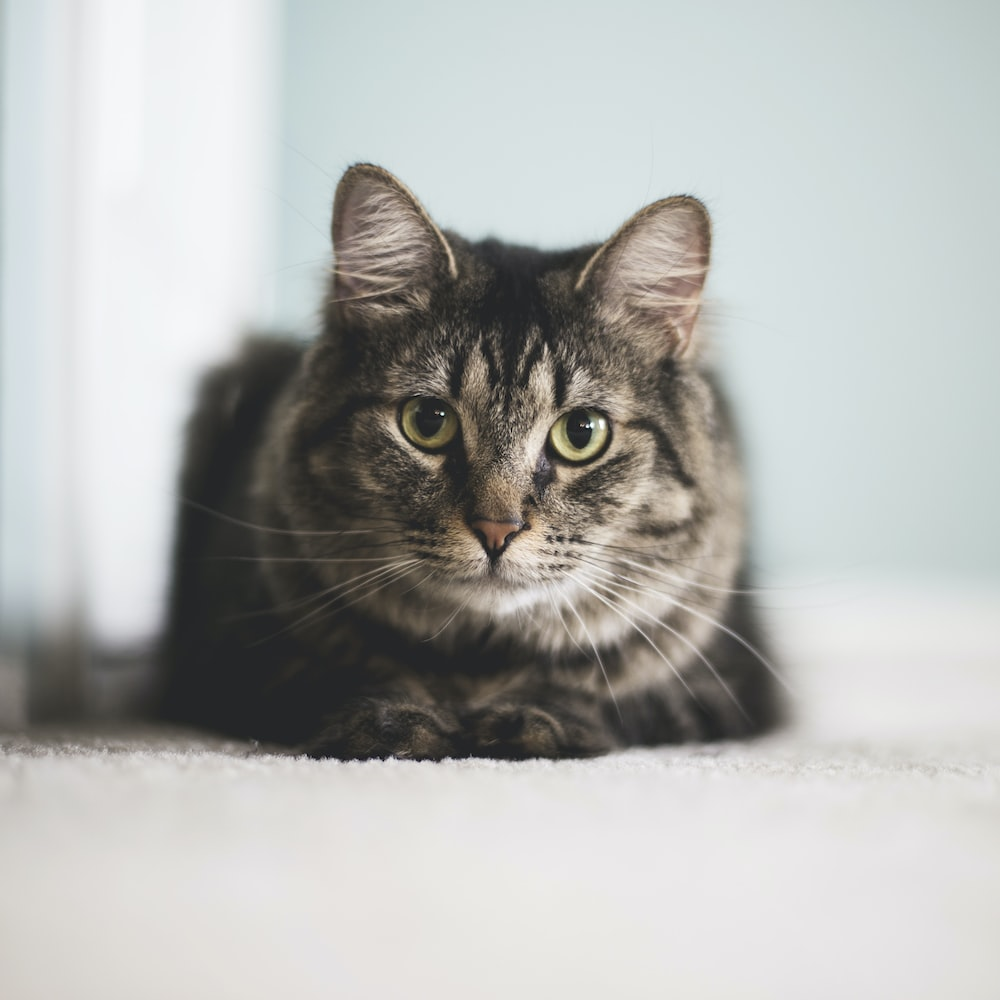
\includegraphics[width=1cm]{data/cat.jpeg}
			};

			\matrix[every node/.style={minimum height=0.15cm, minimum width=0.15cm, draw=black, fill=nodefill, inner sep=0pt}] at (1.65, 0.1) {
				\node{}; \& \node{}; \& \node{}; \& \node{}; \& \node{}; \& \node{}; \& \node{}; \& \node{};\\
				\node{}; \& \node{}; \& \node{}; \& \node{}; \& \node{}; \& \node{}; \& \node{}; \& \node{};\\
				\node{}; \& \node{}; \& \node{}; \& \node{}; \& \node{}; \& \node{}; \& \node{}; \& \node{};\\
				\node{}; \& \node{}; \& \node{}; \& \node{}; \& \node{}; \& \node{}; \& \node{}; \& \node{};\\
				\node{}; \& \node{}; \& \node{}; \& \node{}; \& \node{}; \& \node{}; \& \node{}; \& \node{};\\
				\node{}; \& \node{}; \& \node{}; \& \node{}; \& \node{}; \& \node{}; \& \node{}; \& \node{};\\
				\node{}; \& \node{}; \& \node{}; \& \node{}; \& \node{}; \& \node{}; \& \node{}; \& \node{};\\
				\node{}; \& \node{}; \& \node{}; \& \node{}; \& \node{}; \& \node{}; \& \node{}; \& \node{};\\
			};

			\matrix[every node/.style={minimum height=0.15cm, minimum width=0.15cm, draw=black, fill=nodefill, inner sep=0pt, outer sep=0pt}] (l1) at (1.75, 0) {
				\node{}; \& \node{}; \& \node{}; \& \node{}; \& \node{}; \& \node{}; \& \node{}; \& \node{};\\
				\node{}; \& \node{}; \& \node{}; \& \node{}; \& \node{}; \& \node{}; \& \node{}; \& \node{};\\
				\node{}; \& \node{}; \& \node{}; \& \node{}; \& \node{}; \& \node{}; \& \node{}; \& \node{};\\
				\node{}; \& \node{}; \& \node{}; \& \node{}; \& \node{}; \& \node{}; \& \node{}; \& \node{};\\
				\node{}; \& \node{}; \& \node{}; \& \node{}; \& \node{}; \& \node{}; \& \node{}; \& \node{};\\
				\node{}; \& \node{}; \& \node{}; \& \node{}; \& \node{}; \& \node{}; \& \node{}; \& \node{};\\
				\node{}; \& \node{}; \& \node{}; \& \node{}; \& \node{}; \& \node{}; \& \node{}; \& \node{};\\
				\node{}; \& \node{}; \& \node{}; \& \node{}; \& \node{}; \& \node{}; \& \node{}; \& \node{};\\
			};
			\draw[->] (l0) -- (l1);

			\matrix[every node/.style={minimum height=0.15cm, minimum width=0.15cm, draw=black, fill=nodefill, inner sep=0pt}] at (1.85, -0.1) {
				\node{}; \& \node{}; \& \node{}; \& \node{}; \& \node{}; \& \node{}; \& \node{}; \& \node{};\\
				\node{}; \& \node{}; \& \node{}; \& \node{}; \& \node{}; \& \node{}; \& \node{}; \& \node{};\\
				\node{}; \& \node{}; \& \node{}; \& \node{}; \& \node{}; \& \node{}; \& \node{}; \& \node{};\\
				\node{}; \& \node{}; \& \node{}; \& \node{}; \& \node{}; \& \node{}; \& \node{}; \& \node{};\\
				\node{}; \& \node{}; \& \node{}; \& \node{}; \& \node{}; \& \node{}; \& \node{}; \& \node{};\\
				\node{}; \& \node{}; \& \node{}; \& \node{}; \& \node{}; \& \node{}; \& \node{}; \& \node{};\\
				\node{}; \& \node{}; \& \node{}; \& \node{}; \& \node{}; \& \node{}; \& \node{}; \& \node{};\\
				\node{}; \& \node{}; \& \node{}; \& \node{}; \& \node{}; \& \node{}; \& \node{}; \& \node{};\\
			};

			\matrix[every node/.style={minimum height=0.15cm, minimum width=0.15cm, draw=black, fill=nodefill, inner sep=0pt}] at (3.4, 0.1) {
				\node{}; \& \node{}; \& \node{}; \& \node{}; \& \node{}; \& \node{};\\
				\node{}; \& \node{}; \& \node{}; \& \node{}; \& \node{}; \& \node{};\\
				\node{}; \& \node{}; \& \node{}; \& \node{}; \& \node{}; \& \node{};\\
				\node{}; \& \node{}; \& \node{}; \& \node{}; \& \node{}; \& \node{};\\
				\node{}; \& \node{}; \& \node{}; \& \node{}; \& \node{}; \& \node{};\\
				\node{}; \& \node{}; \& \node{}; \& \node{}; \& \node{}; \& \node{};\\
			};

			\matrix[every node/.style={minimum height=0.15cm, minimum width=0.15cm, draw=black, fill=nodefill, inner sep=0pt}] (l2)at (3.5, 0) {
				\node{}; \& \node{}; \& \node{}; \& \node{}; \& \node{}; \& \node{};\\
				\node{}; \& \node{}; \& \node{}; \& \node{}; \& \node{}; \& \node{};\\
				\node{}; \& \node{}; \& \node{}; \& \node{}; \& \node{}; \& \node{};\\
				\node{}; \& \node{}; \& \node{}; \& \node{}; \& \node{}; \& \node{};\\
				\node{}; \& \node{}; \& \node{}; \& \node{}; \& \node{}; \& \node{};\\
				\node{}; \& \node{}; \& \node{}; \& \node{}; \& \node{}; \& \node{};\\
			};
			\draw[->] (l1) -- (l2);

			\matrix[every node/.style={minimum height=0.15cm, minimum width=0.15cm, draw=black, fill=nodefill, inner sep=0pt}] at (3.6, -0.1) {
				\node{}; \& \node{}; \& \node{}; \& \node{}; \& \node{}; \& \node{};\\
				\node{}; \& \node{}; \& \node{}; \& \node{}; \& \node{}; \& \node{};\\
				\node{}; \& \node{}; \& \node{}; \& \node{}; \& \node{}; \& \node{};\\
				\node{}; \& \node{}; \& \node{}; \& \node{}; \& \node{}; \& \node{};\\
				\node{}; \& \node{}; \& \node{}; \& \node{}; \& \node{}; \& \node{};\\
				\node{}; \& \node{}; \& \node{}; \& \node{}; \& \node{}; \& \node{};\\
			};

			\matrix[every node/.style={minimum height=0.15cm, minimum width=0.15cm, draw=black, fill=nodefill, inner sep=0pt}] at (5.05, 0.2) {
				\node{}; \& \node{}; \& \node{}; \& \node{}; \& \node{}; \& \node{};\\
				\node{}; \& \node{}; \& \node{}; \& \node{}; \& \node{}; \& \node{};\\
				\node{}; \& \node{}; \& \node{}; \& \node{}; \& \node{}; \& \node{};\\
				\node{}; \& \node{}; \& \node{}; \& \node{}; \& \node{}; \& \node{};\\
				\node{}; \& \node{}; \& \node{}; \& \node{}; \& \node{}; \& \node{};\\
				\node{}; \& \node{}; \& \node{}; \& \node{}; \& \node{}; \& \node{};\\
			};

			\matrix[every node/.style={minimum height=0.15cm, minimum width=0.15cm, draw=black, fill=nodefill, inner sep=0pt}] at (5.15, 0.1) {
				\node{}; \& \node{}; \& \node{}; \& \node{}; \& \node{}; \& \node{};\\
				\node{}; \& \node{}; \& \node{}; \& \node{}; \& \node{}; \& \node{};\\
				\node{}; \& \node{}; \& \node{}; \& \node{}; \& \node{}; \& \node{};\\
				\node{}; \& \node{}; \& \node{}; \& \node{}; \& \node{}; \& \node{};\\
				\node{}; \& \node{}; \& \node{}; \& \node{}; \& \node{}; \& \node{};\\
				\node{}; \& \node{}; \& \node{}; \& \node{}; \& \node{}; \& \node{};\\
			};

			\matrix[every node/.style={minimum height=0.15cm, minimum width=0.15cm, draw=black, fill=nodefill, inner sep=0pt}] (l3) at (5.25, 0) {
				\node{}; \& \node{}; \& \node{}; \& \node{}; \& \node{}; \& \node{};\\
				\node{}; \& \node{}; \& \node{}; \& \node{}; \& \node{}; \& \node{};\\
				\node{}; \& \node{}; \& \node{}; \& \node{}; \& \node{}; \& \node{};\\
				\node{}; \& \node{}; \& \node{}; \& \node{}; \& \node{}; \& \node{};\\
				\node{}; \& \node{}; \& \node{}; \& \node{}; \& \node{}; \& \node{};\\
				\node{}; \& \node{}; \& \node{}; \& \node{}; \& \node{}; \& \node{};\\
			};
			\draw[->] (l2) -- ($ (l3.west) - (0.1, 0) $);

			\matrix[every node/.style={minimum height=0.15cm, minimum width=0.15cm, draw=black, fill=nodefill, inner sep=0pt}] at (5.35, -0.1) {
				\node{}; \& \node{}; \& \node{}; \& \node{}; \& \node{}; \& \node{};\\
				\node{}; \& \node{}; \& \node{}; \& \node{}; \& \node{}; \& \node{};\\
				\node{}; \& \node{}; \& \node{}; \& \node{}; \& \node{}; \& \node{};\\
				\node{}; \& \node{}; \& \node{}; \& \node{}; \& \node{}; \& \node{};\\
				\node{}; \& \node{}; \& \node{}; \& \node{}; \& \node{}; \& \node{};\\
				\node{}; \& \node{}; \& \node{}; \& \node{}; \& \node{}; \& \node{};\\
			};

			\matrix[every node/.style={minimum height=0.15cm, minimum width=0.15cm, draw=black, fill=nodefill, inner sep=0pt}] at (5.45, -0.2) {
				\node{}; \& \node{}; \& \node{}; \& \node{}; \& \node{}; \& \node{};\\
				\node{}; \& \node{}; \& \node{}; \& \node{}; \& \node{}; \& \node{};\\
				\node{}; \& \node{}; \& \node{}; \& \node{}; \& \node{}; \& \node{};\\
				\node{}; \& \node{}; \& \node{}; \& \node{}; \& \node{}; \& \node{};\\
				\node{}; \& \node{}; \& \node{}; \& \node{}; \& \node{}; \& \node{};\\
				\node{}; \& \node{}; \& \node{}; \& \node{}; \& \node{}; \& \node{};\\
			};

			\matrix[every node/.style={minimum height=0.15cm, minimum width=0.15cm, draw=black, fill=nodefill, inner sep=0pt}] at (6.8, 0.2) {
				\node{}; \& \node{}; \& \node{}; \& \node{};\\
				\node{}; \& \node{}; \& \node{}; \& \node{};\\
				\node{}; \& \node{}; \& \node{}; \& \node{};\\
				\node{}; \& \node{}; \& \node{}; \& \node{};\\
			};

			\matrix[every node/.style={minimum height=0.15cm, minimum width=0.15cm, draw=black, fill=nodefill, inner sep=0pt}] at (6.9, 0.1) {
				\node{}; \& \node{}; \& \node{}; \& \node{};\\
				\node{}; \& \node{}; \& \node{}; \& \node{};\\
				\node{}; \& \node{}; \& \node{}; \& \node{};\\
				\node{}; \& \node{}; \& \node{}; \& \node{};\\
			};

			\matrix[every node/.style={minimum height=0.15cm, minimum width=0.15cm, draw=black, fill=nodefill, inner sep=0pt}] (l4) at (7, 0) {
				\node{}; \& \node{}; \& \node{}; \& \node{};\\
				\node{}; \& \node{}; \& \node{}; \& \node{};\\
				\node{}; \& \node{}; \& \node{}; \& \node{};\\
				\node{}; \& \node{}; \& \node{}; \& \node{};\\
			};
			\draw[->] ($ (l3.east) + (0.1, 0) $) -- ($ (l4.west) + (-0.1, 0) $);

			\matrix[every node/.style={minimum height=0.15cm, minimum width=0.15cm, draw=black, fill=nodefill, inner sep=0pt}] at (7.1, -0.1) {
				\node{}; \& \node{}; \& \node{}; \& \node{};\\
				\node{}; \& \node{}; \& \node{}; \& \node{};\\
				\node{}; \& \node{}; \& \node{}; \& \node{};\\
				\node{}; \& \node{}; \& \node{}; \& \node{};\\
			};
			\matrix[every node/.style={minimum height=0.15cm, minimum width=0.15cm, draw=black, fill=nodefill, inner sep=0pt}] at (7.2, -0.2) {
				\node{}; \& \node{}; \& \node{}; \& \node{};\\
				\node{}; \& \node{}; \& \node{}; \& \node{};\\
				\node{}; \& \node{}; \& \node{}; \& \node{};\\
				\node{}; \& \node{}; \& \node{}; \& \node{};\\
			};

			\matrix[every node/.style={minimum height=0.15cm, minimum width=0.15cm, draw=black, fill=nodefill, inner sep=0pt}] at (8.25, 0.3) {
				\node{}; \& \node{}; \& \node{}; \& \node{};\\
				\node{}; \& \node{}; \& \node{}; \& \node{};\\
				\node{}; \& \node{}; \& \node{}; \& \node{};\\
				\node{}; \& \node{}; \& \node{}; \& \node{};\\
			};

			\matrix[every node/.style={minimum height=0.15cm, minimum width=0.15cm, draw=black, fill=nodefill, inner sep=0pt}] at (8.35, 0.2) {
				\node{}; \& \node{}; \& \node{}; \& \node{};\\
				\node{}; \& \node{}; \& \node{}; \& \node{};\\
				\node{}; \& \node{}; \& \node{}; \& \node{};\\
				\node{}; \& \node{}; \& \node{}; \& \node{};\\
			};

			\matrix[every node/.style={minimum height=0.15cm, minimum width=0.15cm, draw=black, fill=nodefill, inner sep=0pt}] at (8.45, 0.1) {
				\node{}; \& \node{}; \& \node{}; \& \node{};\\
				\node{}; \& \node{}; \& \node{}; \& \node{};\\
				\node{}; \& \node{}; \& \node{}; \& \node{};\\
				\node{}; \& \node{}; \& \node{}; \& \node{};\\
			};

			\matrix[every node/.style={minimum height=0.15cm, minimum width=0.15cm, draw=black, fill=nodefill, inner sep=0pt}] (l5) at (8.55, 0) {
				\node{}; \& \node{}; \& \node{}; \& \node{};\\
				\node{}; \& \node{}; \& \node{}; \& \node{};\\
				\node{}; \& \node{}; \& \node{}; \& \node{};\\
				\node{}; \& \node{}; \& \node{}; \& \node{};\\
			};
			\draw[->] ($ (l4.east) + (0.1, 0) $) -- ($ (l5.west) + (-0.2, 0) $);

			\matrix[every node/.style={minimum height=0.15cm, minimum width=0.15cm, draw=black, fill=nodefill, inner sep=0pt}] at (8.65, -0.1) {
				\node{}; \& \node{}; \& \node{}; \& \node{};\\
				\node{}; \& \node{}; \& \node{}; \& \node{};\\
				\node{}; \& \node{}; \& \node{}; \& \node{};\\
				\node{}; \& \node{}; \& \node{}; \& \node{};\\
			};

			\matrix[every node/.style={minimum height=0.15cm, minimum width=0.15cm, draw=black, fill=nodefill, inner sep=0pt}] at (8.75, -0.2) {
				\node{}; \& \node{}; \& \node{}; \& \node{};\\
				\node{}; \& \node{}; \& \node{}; \& \node{};\\
				\node{}; \& \node{}; \& \node{}; \& \node{};\\
				\node{}; \& \node{}; \& \node{}; \& \node{};\\
			};

			\matrix[every node/.style={minimum height=0.15cm, minimum width=0.15cm, draw=black, fill=nodefill, inner sep=0pt}] at (8.85, -0.3) {
				\node{}; \& \node{}; \& \node{}; \& \node{};\\
				\node{}; \& \node{}; \& \node{}; \& \node{};\\
				\node{}; \& \node{}; \& \node{}; \& \node{};\\
				\node{}; \& \node{}; \& \node{}; \& \node{};\\
			};


			\node[circle, draw=black, fill=nodefill, text depth=0, inner sep=2pt] (y1) at (10.5, 0.125) {\tiny{$y_0$}};
			\node[circle, draw=black, fill=nodefill, text depth=0, inner sep=2pt] (y2) at (10.75, -0.125) {\tiny{$y_1$}};

			\node[minimum height=0.15cm, minimum width=0.15cm, draw=black, fill=nodefill, inner sep=0pt] (n0) at (9.4, 0.3) {};
			\draw[->] (n0) -- (y1);
			\node[minimum height=0.15cm, minimum width=0.15cm, draw=black, fill=nodefill, inner sep=0pt] (n1) at (9.5, 0.2) {};
			\draw[->] (n1) -- (y1);
			\node[minimum height=0.15cm, minimum width=0.15cm, draw=black, fill=nodefill, inner sep=0pt] (n2) at (9.6, 0.1) {};
			\draw[->] (n2) -- (y1);
			\node[minimum height=0.15cm, minimum width=0.15cm, draw=black, fill=nodefill, inner sep=0pt] (n3) at (9.7, 0) {};
			\draw[->] ($ (l5.east) + (0.2, 0) $) -- ($ (n3.west) + (-0.15, 0) $);
			\draw[->] (n3) -- (y1);
			\node[minimum height=0.15cm, minimum width=0.15cm, draw=black, fill=nodefill, inner sep=0pt] (n4) at (9.8, -0.1) {};
			\draw[->] (n4) -- (y1);
			\node[minimum height=0.15cm, minimum width=0.15cm, draw=black, fill=nodefill, inner sep=0pt] (n5) at (9.9, -0.2) {};
			\draw[->] (n5) -- (y1);
			\node[minimum height=0.15cm, minimum width=0.15cm, draw=black, fill=nodefill, inner sep=0pt] (n6) at (10, -0.3) {};
			\draw[->] (n6) -- (y1);

			\node[minimum height=0.15cm, minimum width=0.15cm, draw=black, fill=nodefill, inner sep=0pt] (n0) at (9.4, 0.3) {};
			\draw[->] (n0) -- (y2);
			\node[minimum height=0.15cm, minimum width=0.15cm, draw=black, fill=nodefill, inner sep=0pt] (n1) at (9.5, 0.2) {};
			\draw[->] (n1) -- (y2);
			\node[minimum height=0.15cm, minimum width=0.15cm, draw=black, fill=nodefill, inner sep=0pt] (n2) at (9.6, 0.1) {};
			\draw[->] (n2) -- (y2);
			\node[minimum height=0.15cm, minimum width=0.15cm, draw=black, fill=nodefill, inner sep=0pt] (n3) at (9.7, 0) {};
			\draw[->] (n3) -- (y2);
			\node[minimum height=0.15cm, minimum width=0.15cm, draw=black, fill=nodefill, inner sep=0pt] (n4) at (9.8, -0.1) {};
			\draw[->] (n4) -- (y2);
			\node[minimum height=0.15cm, minimum width=0.15cm, draw=black, fill=nodefill, inner sep=0pt] (n5) at (9.9, -0.2) {};
			\draw[->] (n5) -- (y2);
			\node[minimum height=0.15cm, minimum width=0.15cm, draw=black, fill=nodefill, inner sep=0pt] (n6) at (10, -0.3) {};
			\draw[->] (n6) -- (y2);

			\draw[-Latex, very thick, red] (9.7, -1) -- (9.7, 0);
			\draw[red, dashed] (9.7, -1.2) -- (9.7, -2.5);

			\node[anchor=east, align=right] at (9.7, -1.85) {\textcolor{red}{Opptrent} \\ \textcolor{red}{mønstergjenkjenning}};
			\node[anchor=west, align=left] at (9.7, -1.85) {\textcolor{red}{Symbolsk} \\ \textcolor{red}{logikk}};

			\node[] at (6, 3) {};
			\node[] at (11, -3) {};

		\end{tikzpicture}
		}
		\vfill
	\end{frame}

	\begin{frame}{Bildegjenkjenning: Oppsummering}
		\begin{itemize}
			\item Moderne bildegjenkjenning gjøres ved hjelp av konvolusjonelle nevrale nettverk.
			\item Konvolusjonelle nevrale nettverk løser oppgaver ved å lære seg å kjenne igjen mønstre i bilder.
			\item Jo lenger inn i nettverket man kommer, jo mer abstrakte og konseptuelle er mønstrene.
		\end{itemize}
	\end{frame}

	\section{Bildegjenkjenning i hjerneforskning}

	\setbeamertemplate{footline}[cole]

	\begin{frame}{Hjernealder}
		\centering
		\vfill
		\begin{tikzpicture}
			\node[
				inner sep=0pt,
				outer sep=0pt,
				draw=black,
				fill=white,
			] at (0, 0) {
				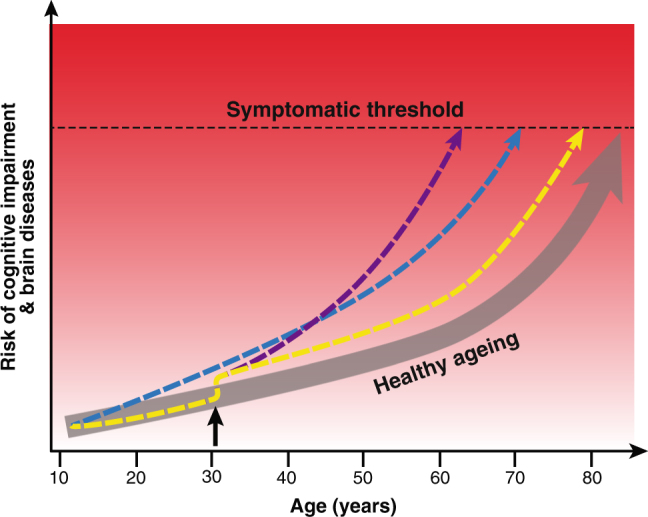
\includegraphics[width=7cm]{data/cole.jpg}
			};
		\end{tikzpicture}
		\vfill
	\end{frame}

	\setbeamertemplate{footline}[deep]

	\begin{frame}{Hjernealder: Datasett}
		\definecolor{hbn-clr}{RGB}{255, 0, 40}
		\definecolor{adhd200-clr}{RGB}{255, 27, 0}
		\definecolor{ping-clr}{RGB}{255, 96, 0}
		\definecolor{ds000119-clr}{RGB}{255, 165, 0}
		\definecolor{abide-clr}{RGB}{255, 234, 0}
		\definecolor{slim-clr}{RGB}{206, 255, 0}
		\definecolor{abide2-clr}{RGB}{137, 255, 0}
		\definecolor{beijing-clr}{RGB}{68, 255, 0}
		\definecolor{aomic-clr}{RGB}{0, 255, 0}
		\definecolor{corr-clr}{RGB}{0, 255, 68}
		\definecolor{mpi-clr}{RGB}{0, 255, 137}
		\definecolor{hcp-clr}{RGB}{0, 255, 205}
		\definecolor{fcon-clr}{RGB}{0, 235, 255}
		\definecolor{nki-clr}{RGB}{0, 166, 255}
		\definecolor{sald-clr}{RGB}{0, 97, 255}
		\definecolor{ds000222-clr}{RGB}{0, 27, 255}
		\definecolor{dlbs-clr}{RGB}{41, 0, 255}
		\definecolor{camcan-clr}{RGB}{110, 0, 255}
		\definecolor{ukb-clr}{RGB}{180, 0, 255}
		\definecolor{oasis-clr}{RGB}{249, 0, 255}
		\definecolor{ds000202-clr}{RGB}{255, 0, 191}

		\centering
		\vfill
		\begin{tikzpicture}
			\begin{axis}[
				width=0.9\textwidth,
				height=0.65\textwidth,
				xmin=0,
				xmax=100,
				ymin=-1200,
				ymax=1200,
				yticklabels={,,},
				ytick=\empty,
				xtick pos=bottom,
				y dir=reverse,
				axis x line=middle,
				axis y line=none,
				xtick={0,10,20,30,40,50,60,70,80}
			]
				\addplot [draw=none, name path=zero] coordinates {
					(0, 0)
					(100, 0)
				};

				\addplot [draw=none, name path=hbn] table [col sep=comma, x=age,y=hbn] {data/paper1/dataset/M.csv};
				\addplot [hbn-clr] fill between [of=zero and hbn];
				\addplot [draw=none, name path=adhd200] table [col sep=comma, x=age,y=adhd200-hc] {data/paper1/dataset/M.csv};
				\addplot [adhd200-clr] fill between [of=hbn and adhd200];\label{trace:adhd200}
				\addplot [draw=none, name path=ping] table [col sep=comma, x=age,y=ping] {data/paper1/dataset/M.csv};
				\addplot [ping-clr] fill between [of=adhd200 and ping];\label{trace:ping}

				\addplot [draw=none, name path=ds000119] table [col sep=comma, x=age,y=ds000119] {data/paper1/dataset/M.csv};
				\addplot [ds000119-clr] fill between [of=ping and ds000119];\label{trace:ds000119}
				\addplot [draw=none, name path=abide] table [col sep=comma, x=age,y=abide-hc] {data/paper1/dataset/M.csv};
				\addplot [abide-clr] fill between [of=ds000119 and abide];\label{trace:abide}
				\addplot [draw=none, name path=slim] table [col sep=comma, x=age,y=slim] {data/paper1/dataset/M.csv};
				\addplot [slim-clr] fill between [of=abide and slim];\label{trace:slim}
				\addplot [draw=none, name path=abide2] table [col sep=comma, x=age,y=abide2-hc] {data/paper1/dataset/M.csv};
				\addplot [abide2-clr] fill between [of=slim and abide2];\label{trace:abide2}
				\addplot [draw=none, name path=beijing] table [col sep=comma, x=age,y=beijing-enhanced] {data/paper1/dataset/M.csv};
				\addplot [beijing-clr] fill between [of=slim and beijing];\label{trace:beijing}
				\addplot [draw=none, name path=aomic] table [col sep=comma, x=age,y=aomic-id1000] {data/paper1/dataset/M.csv};
				\addplot [aomic-clr] fill between [of=beijing and aomic];\label{trace:aomic}
				\addplot [draw=none, name path=corr] table [col sep=comma, x=age,y=corr] {data/paper1/dataset/M.csv};
				\addplot [corr-clr] fill between [of=aomic and corr];\label{trace:corr}
				\addplot [draw=none, name path=mpi] table [col sep=comma, x=age,y=mpi-lemon] {data/paper1/dataset/M.csv};
				\addplot [mpi-clr] fill between [of=corr and mpi];\label{trace:mpi}
				\addplot [draw=none, name path=hcp] table [col sep=comma, x=age,y=hcp] {data/paper1/dataset/M.csv};
				\addplot [hcp-clr] fill between [of=mpi and hcp];\label{trace:hcp}
				\addplot [draw=none, name path=fcon] table [col sep=comma, x=age,y=fcon1000] {data/paper1/dataset/M.csv};
				\addplot [fcon-clr] fill between [of=hcp and fcon];\label{trace:fcon}
				\addplot [draw=none, name path=nki] table [col sep=comma, x=age,y=nki-rockland] {data/paper1/dataset/M.csv};
				\addplot [nki-clr] fill between [of=fcon and nki];\label{trace:nki}
				\addplot [draw=none, name path=sald] table [col sep=comma, x=age,y=sald] {data/paper1/dataset/M.csv};
				\addplot [sald-clr] fill between [of=nki and sald];\label{trace:sald}
				\addplot [draw=none, name path=ds000222] table [col sep=comma, x=age,y=ds000222] {data/paper1/dataset/M.csv};
				\addplot [ds000222-clr] fill between [of=sald and ds000222];\label{trace:ds000222}
				\addplot [draw=none, name path=dlbs] table [col sep=comma, x=age,y=dlbs] {data/paper1/dataset/M.csv};
				\addplot [dlbs-clr] fill between [of=ds000222 and dlbs];\label{trace:dlbs}
				\addplot [draw=none, name path=camcan] table [col sep=comma, x=age,y=camcan] {data/paper1/dataset/M.csv};
				\addplot [camcan-clr] fill between [of=dlbs and camcan];\label{trace:camcan}
				\addplot [draw=none, name path=ukb] table [col sep=comma, x=age,y=ukb] {data/paper1/dataset/M.csv};
				\addplot [ukb-clr] fill between [of=camcan and ukb];\label{trace:ukb}
				\addplot [draw=black, name path=oasis] table [col sep=comma, x=age,y=oasis3-hc] {data/paper1/dataset/M.csv};
				\addplot [oasis-clr] fill between [of=ukb and oasis];\label{trace:oasis}

				\addplot [draw=none, name path=hbn] table [col sep=comma, x=age,y expr=\thisrow{hbn}*-1] {data/paper1/dataset/F.csv};
				\addplot [hbn-clr] fill between [of=zero and hbn];\label{trace:hbn}
				\addplot [draw=none, name path=adhd200] table [col sep=comma, x=age,y=,y expr=\thisrow{adhd200-hc}*-1] {data/paper1/dataset/F.csv};
				\addplot [adhd200-clr] fill between [of=hbn and adhd200];
				\addplot [draw=none, name path=ping] table [col sep=comma, x=age,y expr=\thisrow{ping}*-1] {data/paper1/dataset/F.csv};
				\addplot [ping-clr] fill between [of=adhd200 and ping];
				\addplot [draw=none, name path=abide] table [col sep=comma, x=age,y expr=\thisrow{abide-hc}*-1] {data/paper1/dataset/F.csv};
				\addplot [abide-clr] fill between [of=ping and abide];
				\addplot [draw=none, name path=abide2] table [col sep=comma, x=age,y expr=\thisrow{abide2-hc}*-1] {data/paper1/dataset/F.csv};
				\addplot [abide2-clr] fill between [of=abide and abide2];
				\addplot [draw=none, name path=ds000119] table [col sep=comma, x=age,y=,y expr=\thisrow{ds000119}*-1] {data/paper1/dataset/F.csv};
				\addplot [ds000119-clr] fill between [of=abide2 and ds000119];
				\addplot [draw=none, name path=slim] table [col sep=comma, x=age,y expr=\thisrow{slim}*-1] {data/paper1/dataset/F.csv};
				\addplot [slim-clr] fill between [of=ds000119 and slim];
				\addplot [draw=none, name path=beijing] table [col sep=comma, x=age,y expr=\thisrow{beijing-enhanced}*-1] {data/paper1/dataset/F.csv};
				\addplot [beijing-clr] fill between [of=slim and beijing];
				\addplot [draw=none, name path=ds000202] table [col sep=comma, x=age,y expr=\thisrow{ds000202}*-1] {data/paper1/dataset/F.csv};
				\addplot [ds000202-clr] fill between [of=beijing and ds000202];\label{trace:ds000202}
				\addplot [draw=none, name path=aomic] table [col sep=comma, x=age,y expr=\thisrow{aomic-id1000}*-1] {data/paper1/dataset/F.csv};
				\addplot [aomic-clr] fill between [of=beijing and aomic];
				\addplot [draw=none, name path=mpi] table [col sep=comma, x=age,y expr=\thisrow{mpi-lemon}*-1] {data/paper1/dataset/F.csv};
				\addplot [mpi-clr] fill between [of=aomic and mpi];
				\addplot [draw=none, name path=corr] table [col sep=comma, x=age,y expr=\thisrow{corr}*-1] {data/paper1/dataset/F.csv};
				\addplot [corr-clr] fill between [of=mpi and corr];
				\addplot [draw=none, name path=fcon] table [col sep=comma, x=age,y expr=\thisrow{fcon1000}*-1] {data/paper1/dataset/F.csv};
				\addplot [fcon-clr] fill between [of=corr and fcon];
				\addplot [draw=none, name path=hcp] table [col sep=comma, x=age, y expr=\thisrow{hcp}*-1] {data/paper1/dataset/F.csv};
				\addplot [hcp-clr] fill between [of=fcon and hcp];
				\addplot [draw=none, name path=nki] table [col sep=comma, x=age,y expr=\thisrow{nki-rockland}*-1] {data/paper1/dataset/F.csv};
				\addplot [nki-clr] fill between [of=hcp and nki];
				\addplot [draw=none, name path=ds000222] table [col sep=comma, x=age,y expr=\thisrow{ds000222}*-1] {data/paper1/dataset/F.csv};
				\addplot [ds000222-clr] fill between [of=nki and ds000222];
				\addplot [draw=none, name path=sald] table [col sep=comma, x=age,y expr=\thisrow{sald}*-1] {data/paper1/dataset/F.csv};
				\addplot [sald-clr] fill between [of=ds000222 and sald];
				\addplot [draw=none, name path=camcan] table [col sep=comma, x=age,y expr=\thisrow{camcan}*-1] {data/paper1/dataset/F.csv};
				\addplot [camcan-clr] fill between [of=sald and camcan];
				\addplot [draw=none, name path=dlbs] table [col sep=comma, x=age,y expr=\thisrow{dlbs}*-1] {data/paper1/dataset/F.csv};
				\addplot [dlbs-clr] fill between [of=camcan and dlbs];

				\addplot [draw=none, name path=ukb] table [col sep=comma, x=age,y expr=\thisrow{ukb}*-1] {data/paper1/dataset/F.csv};
				\addplot [ukb-clr] fill between [of=dlbs and ukb];
				\addplot [draw=black, name path=oasis] table [col sep=comma, x=age,y expr=\thisrow{oasis3-hc}*-1] {data/paper1/dataset/F.csv};
				\addplot [oasis-clr] fill between [of=ukb and oasis];

				\addplot [] coordinates {
					(0, 0)
					(100, 0)
				};
				\coordinate (male) at (axis cs:100,35) {};
				\coordinate (female) at (axis cs:100,-35) {};

				\node[] at (50,220) {\textbf{n=53,542}};
			\end{axis}
			\matrix [
				draw=none,
				matrix of nodes,
				anchor=north west,
				row sep=-0.1cm,
				font=\footnotesize,
				column 1/.style={anchor=base west}
			] at (8.2, 6.31) {
				\ref{trace:hbn} HBN \\
				\ref{trace:adhd200} ADHD200 \\
				\ref{trace:ping} PING \\
				\ref{trace:ds000119} ds000119 \\
				\ref{trace:abide} ABIDE \\
				\ref{trace:slim} SLIM \\
				\ref{trace:abide2} ABIDE2 \\
				\ref{trace:beijing} Beijing \\
				\ref{trace:aomic} AOMIC \\
				\ref{trace:corr} CoRR \\
				\ref{trace:mpi} MPI-Lemon \\
				\ref{trace:hcp} HCP \\
				\ref{trace:fcon} FCON1000 \\
				\ref{trace:nki} NKI Rockland \\
				\ref{trace:sald} SALD \\
				\ref{trace:ds000222} ds000222 \\
				\ref{trace:dlbs} DLBS \\
				\ref{trace:camcan} CamCAN \\
				\ref{trace:ukb} UKB \\
				\ref{trace:oasis} OASIS3 \\
				\ref{trace:ds000202} ds000202 \\
			};
			\node [anchor=north east] at (male) {\footnotesize{MALE}};
			\node [anchor=south east] at (female) {\footnotesize{FEMALE}};
		\end{tikzpicture}
		\vfill
	\end{frame}

	\begin{frame}{Hjernealder: Modellering}
        \centering
        \vfill
		\begin{tikzpicture}[scale=0.9]
            \newcommand{\mrivsep}{0.52}
			\newcommand{\mrihsep}{0.44}
			\def\plotwidth{11.68}

			\newcommand{\nodesize}{11pt}
			\newcommand{\hsep}{28pt}
			\newcommand{\vsep}{14pt}

			\newcommand{\arrowwidth}{0.05cm}
			\newcommand{\innerarrow}{{Latex[length=0.1cm, width=0.15cm]}}
			\newcommand{\outerarrow}{{Latex[length=0.2cm, width=0.3cm]}}

			\definecolor{cb-green}{HTML}{4dac93}
			\definecolor{cb-blue}{HTML}{3594d6}
			\definecolor{outercolor}{RGB}{128, 128, 128}
			\colorlet{train-fill}{cb-blue}

			\newcommand{\patientlocation}[1]{($ (1, -1.6) + ####1 $)}
			\newcommand{\controllocation}[1]{($ (1, -2.8) + ####1 $)}
			\newcommand{\modellocation}[1]{($ (0.5 * \plotwidth, -2.2) + ####1 $)}

			\node[draw=none, outer sep=0pt, inner sep=1pt] (input) at \modellocation{(-5 * \hsep, 0)} {
				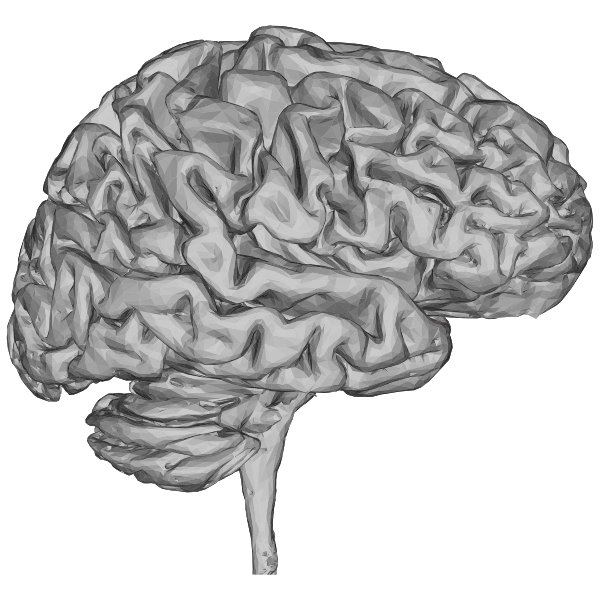
\includegraphics[width=1.5cm] {
					data/brain.png
				}
			};

			\newcommand{\padding}{0.2}

			\draw[] (input.north west) -- ($ (input.north east) - (\padding, 0) $)
					-- ($ (input.south east) - (\padding, -\padding) $)
					-- ($ (input.south west) - (0, -\padding) $)
					-- (input.north west);

			\node[draw=none, outer sep=0pt, inner sep=1pt] (input) at \modellocation{(-5 * \hsep, 0)} {
				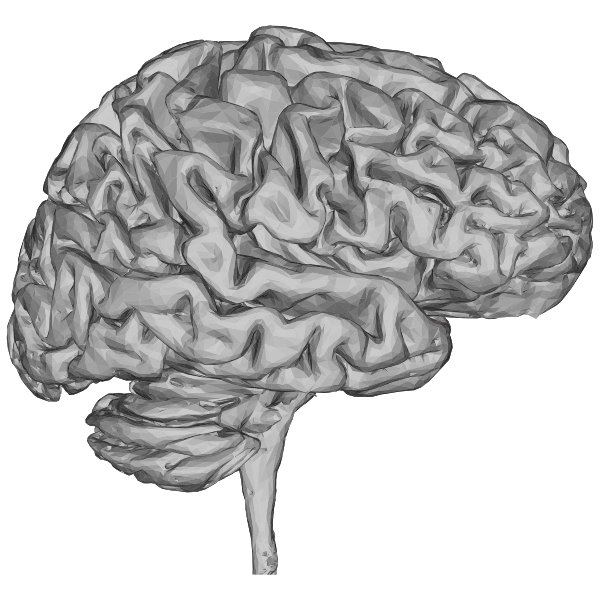
\includegraphics[width=1.5cm] {
					data/brain.png
				}
			};

			\draw[] ($ (input.north west) - (-\padding, \padding) $) -- ($ (input.north east) - (0, \padding) $)
					-- ($ (input.south east) - (0, 0) $)
					-- ($ (input.south west) - (-\padding, 0) $)
					-- ($ (input.north west) - (-\padding, \padding) $);

			\draw[] (input.north west) -- ($ (input.north west) - (-\padding, \padding) $);
			\draw[] ($ (input.south west) - (0, -\padding) $) -- ($ (input.south west) - (-\padding, 0) $);
			\draw[] ($ (input.north east) - (\padding, 0) $) -- ($ (input.north east) - (0, \padding) $);
			\draw[] ($ (input.south east) - (\padding, -\padding) $) -- ($ (input.south east) - (0, 0) $);

			\node[circle, inner sep=0pt, fill=none, outer sep=0pt, line width=0pt, draw=none] (n00) at \modellocation{(-3 * \hsep, 0)} {};

			\node[circle, minimum size=\nodesize, inner sep=0pt, fill=train-fill!35, outer sep=0pt, line width=0pt, draw=train-fill!35] (n10) at \modellocation{(-2 * \hsep, 2 * \vsep)} {};
			\node[circle, minimum size=\nodesize, inner sep=0pt, fill=train-fill, outer sep=0pt, line width=0pt, draw=train-fill] (n11) at \modellocation{(-2 * \hsep, 1 * \vsep)} {};
			\node[circle, minimum size=\nodesize, inner sep=0pt, fill=train-fill!15, outer sep=0pt, line width=0pt, draw=train-fill!15] (n12) at \modellocation{(-2 * \hsep, 0)} {};
			\node[circle, minimum size=\nodesize, inner sep=0pt, fill=train-fill!85, outer sep=0pt, line width=0pt, draw=train-fill!85] (n13) at \modellocation{(-2 * \hsep, -1 * \vsep)} {};
			\node[circle, minimum size=\nodesize, inner sep=0pt, fill=train-fill!90, outer sep=0pt, line width=0pt, draw=train-fill!90] (n14) at \modellocation{(-2 * \hsep, -2 * \vsep)} {};

			\node[circle, minimum size=\nodesize, inner sep=0pt, fill=train-fill!55, outer sep=0pt, line width=0pt, draw=train-fill!55] (n20) at \modellocation{(-1 * \hsep, 1.5 * \vsep)} {};
			\node[circle, minimum size=\nodesize, inner sep=0pt, fill=train-fill!20, outer sep=0pt, line width=0pt, draw=train-fill!20] (n21) at \modellocation{(-1 * \hsep, 0.5 * \vsep)} {};
			\node[circle, minimum size=\nodesize, inner sep=0pt, fill=train-fill!90, outer sep=0pt, line width=0pt, draw=train-fill!50] (n22) at \modellocation{(-1 * \hsep, -0.5 * \vsep)} {};
			\node[circle, minimum size=\nodesize, inner sep=0pt, fill=train-fill!35, outer sep=0pt, line width=0pt, draw=train-fill!35] (n23) at \modellocation{(-1 * \hsep, -1.5 * \vsep)} {};

			\node[circle, minimum size=\nodesize, inner sep=0pt, fill=train-fill!95, outer sep=0pt, line width=0pt, draw=train-fill!65] (n30) at \modellocation{(0 * \hsep, 1.5 * \vsep)} {};
			\node[circle, minimum size=\nodesize, inner sep=0pt, fill=train-fill!20, outer sep=0pt, line width=0pt, draw=train-fill!20] (n31) at \modellocation{(0 * \hsep, 0.5 * \vsep)} {};
			\node[circle, minimum size=\nodesize, inner sep=0pt, fill=train-fill!90, outer sep=0pt, line width=0pt, draw=train-fill!90] (n32) at \modellocation{(0 * \hsep, -0.5 * \vsep)} {};
			\node[circle, minimum size=\nodesize, inner sep=0pt, fill=train-fill!80, outer sep=0pt, line width=0pt, draw=train-fill!80] (n33) at \modellocation{(0 * \hsep, -1.5 * \vsep)} {};

			\node[circle, minimum size=\nodesize, inner sep=0pt, fill=train-fill!50, outer sep=0pt, line width=0pt, draw=train-fill!50] (n40) at \modellocation{(1 * \hsep, 1*\vsep)} {};
			\node[circle, minimum size=\nodesize, inner sep=0pt, fill=train-fill!90, outer sep=0pt, line width=0pt, draw=train-fill!70] (n41) at \modellocation{(1 * \hsep, 0*\vsep)} {};
			\node[circle, minimum size=\nodesize, inner sep=0pt, fill=train-fill!70, outer sep=0pt, line width=0pt, draw=train-fill!30] (n42) at \modellocation{(1 * \hsep, -1*\vsep)} {};

			\node[circle, minimum size=\nodesize, inner sep=0pt, fill=train-fill, outer sep=0pt, line width=0pt, draw=train-fill] (n50) at \modellocation{(2 * \hsep, 1*\vsep)} {};
			\node[circle, minimum size=\nodesize, inner sep=0pt, fill=train-fill!70, outer sep=0pt, line width=0pt, draw=train-fill!70] (n51) at \modellocation{(2 * \hsep, 0*\vsep)} {};
			\node[circle, minimum size=\nodesize, inner sep=0pt, fill=train-fill!30, outer sep=0pt, line width=0pt, draw=train-fill!30] (n52) at \modellocation{(2 * \hsep, -1*\vsep)} {};

			\node[circle, minimum size=\nodesize, inner sep=0pt, fill=train-fill!80, outer sep=0pt, line width=0pt, draw=train-fill!65] (n60) at \modellocation{(3 * \hsep, 0)} {};

			\node[align=left, font=\linespread{0.8}\selectfont] (loss) at (0.5+2.1*4.85, -2.2) {Predikert\\hjernealder};

			\draw[
				color=train-fill!35,
				-\innerarrow,
				line width=\arrowwidth
			] (n00) to [out=20,in=200] (n10) {};
			\draw[
				color=train-fill,
				-\innerarrow,
				line width=\arrowwidth
			] (n00) to [out=10,in=190] (n11) {};
			\draw[
				color=train-fill!15,
				-\innerarrow,
				line width=\arrowwidth
			] (n00) to [out=0,in=180] (n12) {};
			\draw[
				color=train-fill!85,
				-\innerarrow,
				line width=\arrowwidth
			] (n00) to [out=-10,in=170] (n13) {};
			\draw[
				color=train-fill!90,
				-\innerarrow,
				line width=\arrowwidth
			] (n00) to [out=-20,in=160] (n14) {};

			\draw[
				color=train-fill!35,
				-\innerarrow,
				line width=\arrowwidth
			] (n10) to [out=-5,in=175] (n20) {};
			\draw[
				color=train-fill!10,
				-\innerarrow,
				line width=\arrowwidth
			] (n10) to [out=-15,in=165] (n21) {};
			\draw[
				color=train-fill!70,
				-\innerarrow,
				line width=\arrowwidth
			] (n10) to [out=-25,in=155] (n22) {};
			\draw[
				color=train-fill!50,
				-\innerarrow,
				line width=\arrowwidth
			] (n10) to [out=-35,in=145] (n23) {};

			\draw[
				color=train-fill!30,
				-\innerarrow,
				line width=\arrowwidth
			] (n11) to [out=5,in=185] (n20) {};
			\draw[
				color=train-fill!25,
				-\innerarrow,
				line width=\arrowwidth
			] (n11) to [out=-5,in=175] (n21) {};
			\draw[
				color=train-fill!95,
				-\innerarrow,
				line width=\arrowwidth
			] (n11) to [out=-15,in=165] (n22) {};
			\draw[
				color=train-fill!35,
				-\innerarrow,
				line width=\arrowwidth
			] (n11) to [out=-25,in=155] (n23) {};

			\draw[
				color=train-fill!70,
				-\innerarrow,
				line width=\arrowwidth
			] (n12) to [out=15,in=195] (n20) {};
			\draw[
				color=train-fill!20,
				-\innerarrow,
				line width=\arrowwidth
			] (n12) to [out=5,in=185] (n21) {};
			\draw[
				color=train-fill!80,
				-\innerarrow,
				line width=\arrowwidth
			] (n12) to [out=-5,in=175] (n22) {};
			\draw[
				color=train-fill,
				-\innerarrow,
				line width=\arrowwidth
			] (n12) to [out=-15,in=165] (n23) {};

			\draw[
				color=train-fill!40,
				-\innerarrow,
				line width=\arrowwidth
			] (n13) to [out=25,in=205] (n20) {};
			\draw[
				color=train-fill!35,
				-\innerarrow,
				line width=\arrowwidth
			] (n13) to [out=15,in=195] (n21) {};
			\draw[
				color=train-fill!20,
				-\innerarrow,
				line width=\arrowwidth
			] (n13) to [out=5,in=185] (n22) {};
			\draw[
				color=white,
				-\innerarrow,
				line width=\arrowwidth
			] (n13) to [out=-5,in=175] (n23) {};

			\draw[
				color=train-fill!40,
				-\innerarrow,
				line width=\arrowwidth
			] (n14) to [out=35,in=215] (n20) {};
			\draw[
				color=train-fill!85,
				-\innerarrow,
				line width=\arrowwidth
			] (n14) to [out=25,in=205] (n21) {};
			\draw[
				color=train-fill!35,
				-\innerarrow,
				line width=\arrowwidth
			] (n14) to [out=15,in=195] (n22) {};
			\draw[
				color=train-fill,
				-\innerarrow,
				line width=\arrowwidth
			] (n14) to [out=5,in=185] (n23) {};

			\draw[
				color=train-fill!85,
				-\innerarrow,
				line width=\arrowwidth
			] (n20) to [out=0,in=180] (n30) {};
			\draw[
				color=train-fill!50,
				-\innerarrow,
				line width=\arrowwidth
			] (n20) to [out=-10,in=170] (n31) {};
			\draw[
				color=train-fill!75,
				-\innerarrow,
				line width=\arrowwidth
			] (n20) to [out=-20,in=160] (n32) {};
			\draw[
				color=white,
				-\innerarrow,
				line width=\arrowwidth
			] (n20) to [out=-30,in=150] (n33) {};

			\draw[
				color=train-fill,
				-\innerarrow,
				line width=\arrowwidth
			] (n21) to [out=10,in=190] (n30) {};
			\draw[
				color=train-fill!30,
				-\innerarrow,
				line width=\arrowwidth
			] (n21) to [out=0,in=180] (n31) {};
			\draw[
				color=train-fill!25,
				-\innerarrow,
				line width=\arrowwidth
			] (n21) to [out=-10,in=170] (n32) {};
			\draw[
				color=white,
				-\innerarrow,
				line width=\arrowwidth
			] (n21) to [out=-20,in=160] (n33) {};

			\draw[
				color=train-fill!35,
				-\innerarrow,
				line width=\arrowwidth
			] (n22) to [out=20,in=200] (n30) {};
			\draw[
				color=train-fill!95,
				-\innerarrow,
				line width=\arrowwidth
			] (n22) to [out=10,in=190] (n31) {};
			\draw[
				color=train-fill!80,
				-\innerarrow,
				line width=\arrowwidth
			] (n22) to [out=0,in=180] (n32) {};
			\draw[
				color=white,
				-\innerarrow,
				line width=\arrowwidth
			] (n22) to [out=-10,in=170] (n33) {};

			\draw[
				color=train-fill!45,
				-\innerarrow,
				line width=\arrowwidth
			] (n23) to [out=30,in=210] (n30) {};
			\draw[
				color=train-fill!70,
				-\innerarrow,
				line width=\arrowwidth
			] (n23) to [out=20,in=200] (n31) {};
			\draw[
				color=train-fill!10,
				-\innerarrow,
				line width=\arrowwidth
			] (n23) to [out=10,in=190] (n32) {};
			\draw[
				color=train-fill!20,
				-\innerarrow,
				line width=\arrowwidth
			] (n23) to [out=0,in=180] (n33) {};

			\draw[
				color=train-fill!50,
				-\innerarrow,
				line width=\arrowwidth
			] (n30) to [out=-5,in=175] (n40) {};
			\draw[
				color=train-fill!30,
				-\innerarrow,
				line width=\arrowwidth
			] (n30) to [out=-15,in=165] (n41) {};
			\draw[
				color=train-fill,
				-\innerarrow,
				line width=\arrowwidth
			] (n30) to [out=-25,in=155] (n42) {};

			\draw[
				color=train-fill!45,
				-\innerarrow,
				line width=\arrowwidth
			] (n31) to [out=5,in=185] (n40) {};
			\draw[
				color=train-fill!90,
				-\innerarrow,
				line width=\arrowwidth
			] (n31) to [out=-5,in=175] (n41) {};
			\draw[
				color=train-fill!45,
				-\innerarrow,
				line width=\arrowwidth
			] (n31) to [out=-15,in=165] (n42) {};

			\draw[
				color=train-fill!15,
				-\innerarrow,
				line width=\arrowwidth
			] (n32) to [out=15,in=195] (n40) {};
			\draw[
				color=train-fill!70,
				-\innerarrow,
				line width=\arrowwidth
			] (n32) to [out=5,in=185] (n41) {};
			\draw[
				color=train-fill!50,
				-\innerarrow,
				line width=\arrowwidth
			] (n32) to [out=-5,in=175] (n42) {};

			\draw[
				color=train-fill!40,
				-\innerarrow,
				line width=\arrowwidth
			] (n33) to [out=25,in=205] (n40) {};
			\draw[
				color=train-fill!20,
				-\innerarrow,
				line width=\arrowwidth
			] (n33) to [out=15,in=195] (n41) {};
			\draw[
				color=train-fill!90,
				-\innerarrow,
				line width=\arrowwidth
			] (n33) to [out=5,in=185] (n42) {};

			\draw[
				color=train-fill!25,
				-\innerarrow,
				line width=\arrowwidth
			] (n40) to [out=0,in=180] (n50) {};
			\draw[
				color=train-fill!15,
				-\innerarrow,
				line width=\arrowwidth
			] (n40) to [out=-10,in=170] (n51) {};
			\draw[
				color=train-fill,
				-\innerarrow,
				line width=\arrowwidth
			] (n40) to [out=-20,in=160] (n52) {};

			\draw[
				color=train-fill!35,
				-\innerarrow,
				line width=\arrowwidth
			] (n41) to [out=10,in=190] (n50) {};
			\draw[
				color=train-fill!10,
				-\innerarrow,
				line width=\arrowwidth
			] (n41) to [out=0,in=180] (n51) {};
			\draw[
				color=train-fill!90,
				-\innerarrow,
				line width=\arrowwidth
			] (n41) to [out=-10,in=170] (n52) {};

			\draw[
				color=train-fill!50,
				-\innerarrow,
				line width=\arrowwidth
			] (n42) to [out=20,in=200] (n50) {};
			\draw[
				color=train-fill!40,
				-\innerarrow,
				line width=\arrowwidth
			] (n42) to [out=10,in=190] (n51) {};
			\draw[
				color=train-fill!20,
				-\innerarrow,
				line width=\arrowwidth
			] (n42) to [out=0,in=180] (n52) {};

			\draw[
				color=train-fill!80,
				-\innerarrow,
				line width=\arrowwidth,
			] (n50) to [out=-10,in=170] (n60) {};
			\draw[
				color=train-fill!90,
				-\innerarrow,
				line width=\arrowwidth,
			] (n51) to [out=0,in=180] (n60) {};
			\draw[
				color=train-fill!30,
				-\innerarrow,
				line width=\arrowwidth,
			] (n52) to [out=10,in=190] (n60) {};

			\draw[black] (n00.center) --
							($ (n00) + (0, 2*\vsep+0.5*\nodesize+2pt) $) --
							($ (n00) + (6*\hsep+0.5*\nodesize+2pt, 2*\vsep+0.5*\nodesize+2pt) $) --
							($ (n00) + (6*\hsep+0.5*\nodesize+2pt, -2*\vsep-0.5*\nodesize-2pt) $) --
							($ (n00) + (0, -2*\vsep-0.5*\nodesize-2pt) $) --
							(n00.center);

			\node[] at ($ (n30) + (0, \vsep+0.5*\nodesize) $) {Konvolusjonelt nevralt nett};

			\draw[
				color=outercolor,
				-\outerarrow,
				line width=0.1cm
			] ($ (n00.west) - (1, 0) $) to [out=0,in=180] (n00) {};
			\draw[
				color=outercolor,
				-\outerarrow,
				line width=0.1cm
			] (n60) to [out=0,in=180] (loss) {};
		\end{tikzpicture}
        \vfill
	\end{frame}

	\begin{frame}{Hjernealder: Treffsikkerhet}
		\def\N{1}
		\centering
		\vfill
		\begin{tikzpicture}
			\begin{groupplot}[
				group style={
					group size=2 by 1,
					horizontal sep=1.2cm,
					vertical sep=0.8cm
				},
				width=0.5\linewidth,
				height=0.5\linewidth
			]

				\nextgroupplot[
					xmin=0,
					xmax=100,
					ymin=0,
					ymax=100,
					xtick pos=bottom,
					ytick pos=left,
					ticklabel style = {font=\footnotesize},
					xlabel={Kronologisk alder},
					ylabel={Predikert hjernealder},
					title={Testsett}
				]
					\addplot [red] coordinates {(0,0) (100,100)};
					\addplot [
						only marks,
						mark size=1.5pt,
						color=black,
						opacity=0.35
					] table [
						x=regression,
						y=age,
						each nth point={\N},
						col sep=comma
					] {data/paper1/prediction/test_predictions.csv};
					\node [anchor=south east,inner sep=0pt,outer sep=0pt] (outofsample) at (rel axis cs:0.92,0.08) {\textcolor{red}{MAE=2.47}};

				\nextgroupplot[
					xmin=0,
					xmax=100,
					ymin=0,
					ymax=100,
					xtick pos=bottom,
					ytick pos=left,
					ticklabel style = {font=\footnotesize},
					title={Eksternt testsett}
				]
					\addplot [red] coordinates {(0,0) (100,100)};
					\addplot [
						only marks,
						mark size=1.5pt,
						color=black,
						opacity=0.35
					] table [
						x=regression,
						y=age,
						each nth point={\N},
						col sep=comma
					] {data/paper1/prediction/external_predictions.csv};
					\node [anchor=south east,inner sep=0pt,outer sep=0pt] (outofsample) at (rel axis cs:0.92,0.08) {\textcolor{red}{MAE=3.90}};
			\end{groupplot}
	  \end{tikzpicture}
	  \vfill
	\end{frame}

	\begin{frame}{Hjernealder: Assosiasjoner}
		\definecolor{pwas}{HTML}{70F3FF}
		\definecolor{neg}{HTML}{AAFF99}
		\definecolor{pos}{HTML}{FF8585}
		\definecolor{bars}{HTML}{A899FF}

        \centering
        \vfill

  		\begin{columns}[T]
    		\column{0.6\textwidth}
				\begin{tikzpicture}
					\begin{axis}[
							width=1.15\textwidth,
							height=\textwidth,
							ylabel=$-\mathrm{log}_{10}(p)$,
							y label style={at={(-0.06, 0.5)}},
							ymin=0,
							ymax=11.5,
							xmin=-1,
							xmax=395,
							ytick={2,4,6,8,10},
							yticklabels={-2,-4,-6,-8,-10},
							axis x line*=bottom,
							axis y line=left,
							xtick={32.5,102.5,149.5,177.5,208.5,
								233,254.5,275.5,301.5,334.5,
								358,372,388},
							xticklabels={1,2,3,4,5,6,7,8,9,10,
										11,12,13},
							tick label style={font=\scriptsize},
							clip=false,
							xlabel={Categories}
						]
						\addplot[draw=black, only marks, mark size=1.5pt, fill=pwas] table [x=x,y=y,col sep=comma] {data/pwas.csv};
						\addplot[draw=black,dashed] coordinates {(-1, 3.896) (395, 3.896)};
						\addplot[draw=black,dotted] coordinates {(65,0) (65,11.5)};
						\addplot[draw=black,dotted] coordinates {(140,0) (140,11.5)};
						\addplot[draw=black,dotted] coordinates {(159,0) (159,11.5)};
						\addplot[draw=black,dotted] coordinates {(196,0) (196,11.5)};
						\addplot[draw=black,dotted] coordinates {(221,0) (221,11.5)};
						\addplot[draw=black,dotted] coordinates {(245,0) (245,11.5)};
						\addplot[draw=black,dotted] coordinates {(264,0) (264,11.5)};
						\addplot[draw=black,dotted] coordinates {(287,0) (287,11.5)};
						\addplot[draw=black,dotted] coordinates {(316,0) (316,11.5)};
						\addplot[draw=black,dotted] coordinates {(353,0) (353,11.5)};
						\addplot[draw=black,dotted] coordinates {(363,0) (363,11.5)};
						\addplot[draw=black,dotted] coordinates {(381,0) (381,11.5)};
						\addplot[draw=black,dotted] coordinates {(395,0) (395,11.5)};
						\node[anchor=south] at (axis cs:12,6.09) {\tiny{HbA1c}};
						\node[anchor=south] at (axis cs:18,10.49) {\tiny{Glucose}};
						\node[anchor=north] at (axis cs:26,10.23) {\tiny{IGF-1}};
						\node[anchor=south] at (axis cs:49,4.47) {\tiny{Corpuscular volume}};
						\node[anchor=south, align=center] at (axis cs:65,6.72) {\tiny{Vascular/heart}\\[-1.5ex] \tiny{problem}};
						\node[anchor=south, align=center] at (axis cs:89,9.93) {\tiny{Blood pressure}\\[-1.5ex] \tiny{medication}};
						\node[anchor=south] at (axis cs:128,6.64) {\tiny{Diabetes}};
						\node[anchor=south] at (axis cs:254,6.94) {\tiny{Weekly beer/cider intake}};
						\node[anchor=south, align=center] at (axis cs:303,4.61) {\tiny{Total cigarette}\\[-1.5ex] \tiny{packs}};
						\node[anchor=south, align=center] at (axis cs:376,5.33) {\tiny{Non-UK country}\\[-1.5ex] \tiny{of birth}};
					\end{axis}
				\end{tikzpicture}

			\column{0.4\textwidth} % Adjust the width of the second column
				%\vspace*{-0.35cm}
				\begin{tikzpicture}
					\begin{groupplot}[
						group style={
									group size=2 by 1,
									horizontal sep=2cm
								},
								width=0.6\textwidth,
								height=1.5\textwidth,
						]
						\nextgroupplot[
							yticklabels={,,},
							xmin=-1,
							xmax=0,
							xtick={0, -0.5, -1},
							ymin=0,
							ymax=19,
							axis x line=bottom,
							axis y line*=right,
							x axis line style={stealth-},
							ymajorticks=false,
							tick label style={font=\scriptsize}
						]
							\addplot[fill=neg] coordinates {
								(0,0.1)
								(0,0.9)
								(-0.627,0.9)
								(-0.627,0.1)
								(0,0.1)
							};

							\addplot[fill=neg] coordinates {
								(0,1.1)
								(0,1.9)
								(-0.272,1.9)
								(-0.272,1.1)
								(0,1.1)
							};

							\addplot[fill=neg] coordinates {
								(0,2.1)
								(0,2.9)
								(-0.225,2.9)
								(-0.225,2.1)
								(0,2.1)
							};

							\addplot[fill=neg] coordinates {
								(0,3.1)
								(0,3.9)
								(-0.166,3.9)
								(-0.166,3.1)
								(0,3.1)
							};

							\addplot[fill=neg] coordinates {
								(0,4.1)
								(0,4.9)
								(-0.136,4.9)
								(-0.136,4.1)
								(0,4.1)
							};

							\coordinate (1) at (axis cs: 0.99,0.5) {};
							\coordinate (2) at (axis cs: 0.99,1.5) {};
							\coordinate (3) at (axis cs: 0.99,2.5) {};
							\coordinate (4) at (axis cs: 0.99,3.5) {};
							\coordinate (5) at (axis cs: 0.99,4.5) {};
							\coordinate (6) at (axis cs: 0.99,5.5) {};
							\coordinate (7) at (axis cs: 0.99,6.5) {};
							\coordinate (8) at (axis cs: 0.99,7.5) {};
							\coordinate (9) at (axis cs: 0.99,8.5) {};
							\coordinate (10) at (axis cs: 0.99,9.5) {};
							\coordinate (11) at (axis cs: 0.99,10.5) {};
							\coordinate (12) at (axis cs: 0.99,11.5) {};
							\coordinate (13) at (axis cs: 0.99,12.5) {};
							\coordinate (14) at (axis cs: 0.99,13.5) {};
							\coordinate (15) at (axis cs: 0.99,14.5) {};
							\coordinate (16) at (axis cs: 0.99,15.5) {};
							\coordinate (17) at (axis cs: 0.99,16.5) {};
							\coordinate (18) at (axis cs: 0.99,17.5) {};
							\coordinate (19) at (axis cs: 0.99,18.5) {};
						\nextgroupplot[
							yticklabels={,,},
							xmin=0,
							xmax=2,
							ymin=0,
							ymax=19,
							axis x line=bottom,
							axis y line*=left,
							ymajorticks=false,,
							tick label style={font=\scriptsize}
						]

							\addplot[fill=pos] coordinates {
								(0,5.1)
								(0,5.9)
								(0.127,5.9)
								(0.127,5.1)
								(0,5.1)
							};

							\addplot[fill=pos] coordinates {
								(0,6.1)
								(0,6.9)
								(0.137,6.9)
								(0.137,6.1)
								(0,6.1)
							};

							\addplot[fill=pos] coordinates {
								(0,7.1)
								(0,7.9)
								(0.156,7.9)
								(0.156,7.1)
								(0,7.1)
							};

							\addplot[fill=pos] coordinates {
								(0,8.1)
								(0,8.9)
								(0.161,8.9)
								(0.161,8.1)
								(0,8.1)
							};

							\addplot[fill=pos] coordinates {
								(0,9.1)
								(0,9.9)
								(0.169,9.9)
								(0.169,9.1)
								(0,9.1)
							};

							\addplot[fill=pos] coordinates {
								(0,10.1)
								(0,10.9)
								(0.211,10.9)
								(0.211,10.1)
								(0,10.1)
							};

							\addplot[fill=pos] coordinates {
								(0,11.1)
								(0,11.9)
								(0.230,11.9)
								(0.230,11.1)
								(0,11.1)
							};

							\addplot[fill=pos] coordinates {
								(0,12.1)
								(0,12.9)
								(0.246,12.9)
								(0.246,12.1)
								(0,12.1)
							};

							\addplot[fill=pos] coordinates {
								(0,13.1)
								(0,13.9)
								(0.251,13.9)
								(0.251,13.1)
								(0,13.1)
							};

							\addplot[fill=pos] coordinates {
								(0,14.1)
								(0,14.9)
								(0.265,14.9)
								(0.265,14.1)
								(0,14.1)
							};

							\addplot[fill=pos] coordinates {
								(0,15.1)
								(0,15.9)
								(0.415,15.9)
								(0.415,15.1)
								(0,15.1)
							};

							\addplot[fill=pos] coordinates {
								(0,16.1)
								(0,16.9)
								(0.540,16.9)
								(0.540,16.1)
								(0,16.1)
							};

							\addplot[fill=pos] coordinates {
								(0,17.1)
								(0,17.9)
								(0.74,17.9)
								(0.74,17.1)
								(0,17.1)
							};

							\addplot[fill=pos] coordinates {
								(0,18.1)
								(0,18.9)
								(1.786,18.9)
								(1.786,18.1)
								(0,18.1)
							};

					\end{groupplot}
					\node [align=center] at ($ (1) - (0, 0.6) $) {Effect sizes};
					\node [align=center,font=\tiny\linespread{0.8}\selectfont] at (1) {Non-UK country of birth};
					\node [align=center,font=\tiny\linespread{0.8}\selectfont] at (2) {Other group activity};
					\node [align=center,font=\tiny\linespread{0.8}\selectfont] at (3) {IGF-1};
					\node [align=center,font=\tiny\linespread{0.8}\selectfont] at (4) {Cereal intake};
					\node [align=center,font=\tiny\linespread{0.8}\selectfont] at (5) {Number in household};
					\node [align=center,font=\tiny\linespread{0.8}\selectfont] at (6) {Alcohol intake freq.};
					\node [align=center,font=\tiny\linespread{0.8}\selectfont] at (7) {Corpuscular volume};
					\node [align=center,font=\tiny\linespread{0.8}\selectfont] at (8) {Diastolic BP};
					\node [align=center,font=\tiny\linespread{0.8}\selectfont] at (9) {Systolic BP};
					\node [align=center,font=\tiny\linespread{0.8}\selectfont] at (10) {HbA1c};
					\node [align=center,font=\tiny\linespread{0.8}\selectfont] at (11) {Weekly beer/cider intake};
					\node [align=center,font=\tiny\linespread{0.8}\selectfont] at (12) {Glucose};
					\node [align=center,font=\tiny\linespread{0.8}\selectfont] at (13) {Total cigarette packs};
					\node [align=center,font=\tiny\linespread{0.8}\selectfont] at (14) {Age stopped smoking};
					\node [align=center,font=\tiny\linespread{0.8}\selectfont] at (15) {Cigarette packs per year};
					\node [align=center,font=\tiny\linespread{0.8}\selectfont] at (16) {Vascular/heart problem};
					\node [align=center,font=\tiny\linespread{0.8}\selectfont] at (17) {BP medication};
					\node [align=center,font=\tiny\linespread{0.8}\selectfont] at (18) {Diabetes};
					\node [align=center,font=\tiny\linespread{0.8}\selectfont] at (19) {Diabetic retinopathy};
        		\end{tikzpicture}
		\end{columns}
		\vfill
	\end{frame}

	\begin{frame}{Hjernealder: Pasientgrupper}
        \centering
        \vfill
		\begin{figure}
			\begin{center}
				\begin{tikzpicture}
					\begin{axis}[
						height=0.7\textwidth,
						width=0.7\textwidth,
						axis x line=bottom,
						hide y axis,
						xmin=-19,
						xmax=19,
						ymin=-0.1,
						ymax=6.6,
						xlabel=Brain age delta,
						axis line style={latex-latex}
					]
						\addplot [black, dashed] coordinates {(0,-0.3) (0,9)};

						\addplot [blue,very thick,name path=MScontrols] table [x=x,y expr=\thisrow{control} + 5.5,col sep=comma] {data/paper1/supplementary/MS/delta_distributions.csv};
						\addplot [red,very thick,name path=MSpatients] table [x=x,y expr=\thisrow{patient} + 5.5,col sep=comma] {data/paper1/supplementary/MS/delta_distributions.csv};
						\addplot [draw=none,name path=MSbaseline] coordinates {(-20,5.5) (20,5.5)};
						\addplot [blue,fill opacity=0.3] fill between [of=MScontrols and MSbaseline];
						\addplot [red,fill opacity=0.3] fill between [of=MSpatients and MSbaseline];
						\coordinate (MS) at (axis cs:19,6.7) {};
						\addplot [blue,very thick,name path=ADcontrols] table [x=x,y expr=\thisrow{control} + 4.4,col sep=comma] {data/paper1/supplementary/AD/delta_distributions.csv};
						\addplot [red,very thick,name path=ADpatients] table [x=x,y expr=\thisrow{patient} + 4.4,col sep=comma] {data/paper1/supplementary/AD/delta_distributions.csv};
						\addplot [draw=none,name path=ADbaseline] coordinates {(-20,4.4) (20,4.4)};
						\addplot [blue,fill opacity=0.3] fill between [of=ADcontrols and ADbaseline];
						\addplot [red,fill opacity=0.3] fill between [of=ADpatients and ADbaseline];
						\coordinate (AD) at (axis cs:19,5.6) {};
						\addplot [blue,very thick,name path=MCIcontrols] table [x=x,y expr=\thisrow{control} + 3.3,col sep=comma] {data/paper1/supplementary/MCI/delta_distributions.csv};
						\addplot [red,very thick,name path=MCIpatients] table [x=x,y expr=\thisrow{patient} + 3.3,col sep=comma] {data/paper1/supplementary/MCI/delta_distributions.csv};
						\addplot [draw=none,name path=MCIbaseline] coordinates {(-20,3.3) (20,3.3)};
						\addplot [blue,fill opacity=0.3] fill between [of=MCIcontrols and MCIbaseline];
						\addplot [red,fill opacity=0.3] fill between [of=MCIpatients and MCIbaseline];
						\coordinate (MCI) at (axis cs:19,4.5) {};
						\addplot [blue,very thick,name path=SCZcontrols] table [x=x,y expr=\thisrow{control} + 2.2,col sep=comma] {data/paper1/supplementary/SCZ/delta_distributions.csv};
						\addplot [red,very thick,name path=SCZpatients] table [x=x,y expr=\thisrow{patient} + 2.2,col sep=comma] {data/paper1/supplementary/SCZ/delta_distributions.csv};
						\addplot [draw=none,name path=SCZbaseline] coordinates {(-20,2.2) (20,2.2)};
						\addplot [blue,fill opacity=0.3] fill between [of=SCZcontrols and SCZbaseline];
						\addplot [red,fill opacity=0.3] fill between [of=SCZpatients and SCZbaseline];
						\coordinate (SCZ) at (axis cs:19,3.4) {};
						\addplot [blue,very thick,name path=PSYcontrols] table [x=x,y expr=\thisrow{control} + 1.1,col sep=comma] {data/paper1/supplementary/PSY/delta_distributions.csv};
						\addplot [red,very thick,name path=PSYpatients] table [x=x,y expr=\thisrow{patient} + 1.1,col sep=comma] {data/paper1/supplementary/PSY/delta_distributions.csv};
						\addplot [draw=none,name path=PSYbaseline] coordinates {(-20,1.1) (20,1.1)};
						\addplot [blue,fill opacity=0.3] fill between [of=PSYcontrols and PSYbaseline];
						\addplot [red,fill opacity=0.3] fill between [of=PSYpatients and PSYbaseline];
						\coordinate (PSY) at (axis cs:19,2.3) {};
						\addplot [blue,very thick,name path=MOODcontrols] table [x=x,y expr=\thisrow{control},col sep=comma] {data/paper1/supplementary/MOOD/delta_distributions.csv};
						\addplot [red,very thick,name path=MOODpatients] table [x=x,y expr=\thisrow{patient},col sep=comma] {data/paper1/supplementary/MOOD/delta_distributions.csv};
						\addplot [draw=none,name path=MOODbaseline] coordinates {(-20,0) (20,0)};
						\addplot [blue,fill opacity=0.3] fill between [of=MOODcontrols and MOODbaseline];
						\addplot [red,fill opacity=0.3] fill between [of=MOODpatients and MOODbaseline];
						\coordinate (MOOD) at (axis cs:19,1.2) {};
					\end{axis}
					\matrix [
						matrix of nodes,
						draw=none,
						row sep=-0.15cm,
						anchor=north west,
						column 1/.style={anchor=base west, nodes={font=\tiny}}
					] at (MS) {
						\textbf{\underline{MS}} \\
						$\Delta=4.42$\\
						$p=1.71*10^{-22}$\\
						$d=0.87$\\
					};
					\matrix [
						matrix of nodes,
						draw=none,
						row sep=-0.15cm,
						anchor=north west,
						column 1/.style={anchor=base west, nodes={font=\tiny}}
					] at (AD) {
						\textbf{\underline{AD}} \\
						$\Delta=2.81$\\
						$p=4.27*10^{-20}$\\
						$d=0.58$\\
					};
					\matrix [
						matrix of nodes,
						draw=none,
						row sep=-0.15cm,
						anchor=north west,
						column 1/.style={anchor=base west, nodes={font=\tiny}}
					] at (MCI) {
						\textbf{\underline{MCI}} \\
						$\Delta=2.13$\\
						$p=1.25*10^{-15}$\\
						$d=0.46$\\
					};
					\matrix [
						matrix of nodes,
						draw=none,
						row sep=-0.15cm,
						anchor=north west,
						column 1/.style={anchor=base west, nodes={font=\tiny}}
					] at (SCZ) {
						\textbf{\underline{SCZ}} \\
						$\Delta=1.40$\\
						$p=4.29*10^{-5}$\\
						$d=0.34$\\
					};
					\matrix [
						matrix of nodes,
						draw=none,
						row sep=-0.15cm,
						anchor=north west,
						column 1/.style={anchor=base west, nodes={font=\tiny}}
					] at (PSY) {
						\textbf{\underline{PSY}} \\
						$\Delta=0.74$\\
						$p=0.15$\textcolor{white}{$5^2$}\\
						$d=0.20$\\
					};
					\matrix [
						matrix of nodes,
						draw=none,
						row sep=-0.15cm,
						anchor=north west,
						column 1/.style={anchor=base west, nodes={font=\tiny}}
					] at (MOOD) {
						\textbf{\underline{MOOD}} \\
						$\Delta=0.64$\\
						$p=0.04$\textcolor{white}{$5^2$}\\
						$d=0.17$\\
					};

				\end{tikzpicture}
			\end{center}
		\end{figure}
        \vfill
	\end{frame}

	\setbeamertemplate{footline}[default]

	\definecolor{train-fill}{HTML}{0079FF}

	% XAI: ANNs
	\begin{frame}{Forklarbar AI: Layerwise relevance propagation}
		\begin{tikzpicture}
			\newcommand{\nodesize}{8pt}
			\newcommand{\hsep}{24pt}
			\newcommand{\vsep}{12pt}

			\newcommand{\arrowwidth}{0.05cm}
			\newcommand{\innerarrow}{{Latex[length=0.1cm, width=0.15cm]}}

			\newcommand{\modellocation}[1]{($ (0, 0) + ####1 $)}

			\node[circle, inner sep=0pt, fill=none, outer sep=0pt, line width=0pt, draw=none] (n00) at \modellocation{(-3 * \hsep, 0)} {};
			\node[] at (-5.5, 1.5) {};
			\node[] at (5.1, -1.2) {};

			\draw[black, fill=gray!20] (n00.center) --
							($ (n00) + (0, 2*\vsep+0.5*\nodesize+2pt) $) --
							($ (n00) + (6*\hsep+0.5*\nodesize+2pt, 2*\vsep+0.5*\nodesize+2pt) $) --
							($ (n00) + (6*\hsep+0.5*\nodesize+2pt, -2*\vsep-0.5*\nodesize-2pt) $) --
							($ (n00) + (0, -2*\vsep-0.5*\nodesize-2pt) $) --
							(n00.center);


			\node[circle, draw=black, minimum size=\nodesize, inner sep=0pt, fill=gray, outer sep=0pt, line width=0pt, draw=gray] (n10) at \modellocation{(-2 * \hsep, 2 * \vsep)} {};
			\node[circle, minimum size=\nodesize, inner sep=0pt, fill=gray, outer sep=0pt, line width=0pt, draw=gray] (n11) at \modellocation{(-2 * \hsep, 1 * \vsep)} {};
			\node[circle, minimum size=\nodesize, inner sep=0pt, fill=gray, outer sep=0pt, line width=0pt, draw=gray] (n12) at \modellocation{(-2 * \hsep, 0)} {};
			\node[circle, minimum size=\nodesize, inner sep=0pt, fill=gray, outer sep=0pt, line width=0pt, draw=gray] (n13) at \modellocation{(-2 * \hsep, -1 * \vsep)} {};
			\node[circle, minimum size=\nodesize, inner sep=0pt, fill=gray, outer sep=0pt, line width=0pt, draw=gray] (n14) at \modellocation{(-2 * \hsep, -2 * \vsep)} {};

			\node[circle, minimum size=\nodesize, inner sep=0pt, fill=gray, outer sep=0pt, line width=0pt, draw=gray] (n20) at \modellocation{(-1 * \hsep, 1.5 * \vsep)} {};
			\node[circle, minimum size=\nodesize, inner sep=0pt, fill=gray, outer sep=0pt, line width=0pt, draw=gray] (n21) at \modellocation{(-1 * \hsep, 0.5 * \vsep)} {};
			\node[circle, minimum size=\nodesize, inner sep=0pt, fill=gray, outer sep=0pt, line width=0pt, draw=gray] (n22) at \modellocation{(-1 * \hsep, -0.5 * \vsep)} {};
			\node[circle, minimum size=\nodesize, inner sep=0pt, fill=gray, outer sep=0pt, line width=0pt, draw=gray] (n23) at \modellocation{(-1 * \hsep, -1.5 * \vsep)} {};

			\node[circle, minimum size=\nodesize, inner sep=0pt, fill=gray, outer sep=0pt, line width=0pt, draw=gray] (n30) at \modellocation{(0 * \hsep, 1.5 * \vsep)} {};
			\node[circle, minimum size=\nodesize, inner sep=0pt, fill=gray, outer sep=0pt, line width=0pt, draw=gray] (n31) at \modellocation{(0 * \hsep, 0.5 * \vsep)} {};
			\node[circle, minimum size=\nodesize, inner sep=0pt, fill=gray, outer sep=0pt, line width=0pt, draw=gray] (n32) at \modellocation{(0 * \hsep, -0.5 * \vsep)} {};
			\node[circle, minimum size=\nodesize, inner sep=0pt, fill=gray, outer sep=0pt, line width=0pt, draw=gray] (n33) at \modellocation{(0 * \hsep, -1.5 * \vsep)} {};

			\node[circle, minimum size=\nodesize, inner sep=0pt, fill=gray, outer sep=0pt, line width=0pt, draw=gray] (n40) at \modellocation{(1 * \hsep, 1*\vsep)} {};
			\node[circle, minimum size=\nodesize, inner sep=0pt, fill=gray, outer sep=0pt, line width=0pt, draw=gray] (n41) at \modellocation{(1 * \hsep, 0*\vsep)} {};
			\node[circle, minimum size=\nodesize, inner sep=0pt, fill=gray, outer sep=0pt, line width=0pt, draw=gray] (n42) at \modellocation{(1 * \hsep, -1*\vsep)} {};

			\node[circle, minimum size=\nodesize, inner sep=0pt, fill=gray, outer sep=0pt, line width=0pt, draw=gray] (n50) at \modellocation{(2 * \hsep, 1*\vsep)} {};
			\node[circle, minimum size=\nodesize, inner sep=0pt, fill=gray, outer sep=0pt, line width=0pt, draw=gray] (n51) at \modellocation{(2 * \hsep, 0*\vsep)} {};
			\node[circle, minimum size=\nodesize, inner sep=0pt, fill=gray, outer sep=0pt, line width=0pt, draw=gray] (n52) at \modellocation{(2 * \hsep, -1*\vsep)} {};

			\node[circle, minimum size=\nodesize, inner sep=0pt, fill=gray, outer sep=0pt, line width=0pt, draw=gray] (n60) at \modellocation{(3 * \hsep, 0)} {};

			\draw[
				color=gray!70,
				-\innerarrow,
				line width=\arrowwidth
			] (n00) to [out=20,in=200] (n10) {};
			\draw[
				color=gray!70,
				-\innerarrow,
				line width=\arrowwidth
			] (n00) to [out=10,in=190] (n11) {};
			\draw[
				color=gray!70,
				-\innerarrow,
				line width=\arrowwidth
			] (n00) to [out=0,in=180] (n12) {};
			\draw[
				color=gray!70,
				-\innerarrow,
				line width=\arrowwidth
			] (n00) to [out=-10,in=170] (n13) {};
			\draw[
				color=gray!70,
				-\innerarrow,
				line width=\arrowwidth
			] (n00) to [out=-20,in=160] (n14) {};

			\draw[
				color=gray!70,
				-\innerarrow,
				line width=\arrowwidth
			] (n10) to [out=-5,in=175] (n20) {};
			\draw[
				color=gray!70,
				-\innerarrow,
				line width=\arrowwidth
			] (n10) to [out=-15,in=165] (n21) {};
			\draw[
				color=gray!70,
				-\innerarrow,
				line width=\arrowwidth
			] (n10) to [out=-25,in=155] (n22) {};
			\draw[
				color=gray!70,
				-\innerarrow,
				line width=\arrowwidth
			] (n10) to [out=-35,in=145] (n23) {};

			\draw[
				color=gray!70,
				-\innerarrow,
				line width=\arrowwidth
			] (n11) to [out=5,in=185] (n20) {};
			\draw[
				color=gray!70,
				-\innerarrow,
				line width=\arrowwidth
			] (n11) to [out=-5,in=175] (n21) {};
			\draw[
				color=gray!70,
				-\innerarrow,
				line width=\arrowwidth
			] (n11) to [out=-15,in=165] (n22) {};
			\draw[
				color=gray!70,
				-\innerarrow,
				line width=\arrowwidth
			] (n11) to [out=-25,in=155] (n23) {};

			\draw[
				color=gray!70,
				-\innerarrow,
				line width=\arrowwidth
			] (n12) to [out=15,in=195] (n20) {};
			\draw[
				color=gray!70,
				-\innerarrow,
				line width=\arrowwidth
			] (n12) to [out=5,in=185] (n21) {};
			\draw[
				color=gray!70,
				-\innerarrow,
				line width=\arrowwidth
			] (n12) to [out=-5,in=175] (n22) {};
			\draw[
				color=gray!70,
				-\innerarrow,
				line width=\arrowwidth
			] (n12) to [out=-15,in=165] (n23) {};

			\draw[
				color=gray!70,
				-\innerarrow,
				line width=\arrowwidth
			] (n13) to [out=25,in=205] (n20) {};
			\draw[
				color=gray!70,
				-\innerarrow,
				line width=\arrowwidth
			] (n13) to [out=15,in=195] (n21) {};
			\draw[
				color=gray!70,
				-\innerarrow,
				line width=\arrowwidth
			] (n13) to [out=5,in=185] (n22) {};
			\draw[
				color=gray!70,
				-\innerarrow,
				line width=\arrowwidth
			] (n13) to [out=-5,in=175] (n23) {};

			\draw[
				color=gray!70,
				-\innerarrow,
				line width=\arrowwidth
			] (n14) to [out=35,in=215] (n20) {};
			\draw[
				color=gray!70,
				-\innerarrow,
				line width=\arrowwidth
			] (n14) to [out=25,in=205] (n21) {};
			\draw[
				color=gray!70,
				-\innerarrow,
				line width=\arrowwidth
			] (n14) to [out=15,in=195] (n22) {};
			\draw[
				color=gray!70,
				-\innerarrow,
				line width=\arrowwidth
			] (n14) to [out=5,in=185] (n23) {};

			\draw[
				color=gray!70,
				-\innerarrow,
				line width=\arrowwidth
			] (n20) to [out=0,in=180] (n30) {};
			\draw[
				color=gray!70,
				-\innerarrow,
				line width=\arrowwidth
			] (n20) to [out=-10,in=170] (n31) {};
			\draw[
				color=gray!70,
				-\innerarrow,
				line width=\arrowwidth
			] (n20) to [out=-20,in=160] (n32) {};
			\draw[
				color=gray!70,
				-\innerarrow,
				line width=\arrowwidth
			] (n20) to [out=-30,in=150] (n33) {};

			\draw[
				color=gray!70,
				-\innerarrow,
				line width=\arrowwidth
			] (n21) to [out=10,in=190] (n30) {};
			\draw[
				color=gray!70,
				-\innerarrow,
				line width=\arrowwidth
			] (n21) to [out=0,in=180] (n31) {};
			\draw[
				color=gray!70,
				-\innerarrow,
				line width=\arrowwidth
			] (n21) to [out=-10,in=170] (n32) {};
			\draw[
				color=gray!70,
				-\innerarrow,
				line width=\arrowwidth
			] (n21) to [out=-20,in=160] (n33) {};

			\draw[
				color=gray!70,
				-\innerarrow,
				line width=\arrowwidth
			] (n22) to [out=20,in=200] (n30) {};
			\draw[
				color=gray!70,
				-\innerarrow,
				line width=\arrowwidth
			] (n22) to [out=10,in=190] (n31) {};
			\draw[
				color=gray!70,
				-\innerarrow,
				line width=\arrowwidth
			] (n22) to [out=0,in=180] (n32) {};
			\draw[
				color=gray!70,
				-\innerarrow,
				line width=\arrowwidth
			] (n22) to [out=-10,in=170] (n33) {};

			\draw[
				color=gray!70,
				-\innerarrow,
				line width=\arrowwidth
			] (n23) to [out=30,in=210] (n30) {};
			\draw[
				color=gray!70,
				-\innerarrow,
				line width=\arrowwidth
			] (n23) to [out=20,in=200] (n31) {};
			\draw[
				color=gray!70,
				-\innerarrow,
				line width=\arrowwidth
			] (n23) to [out=10,in=190] (n32) {};
			\draw[
				color=gray!70,
				-\innerarrow,
				line width=\arrowwidth
			] (n23) to [out=0,in=180] (n33) {};

			\draw[
				color=gray!70,
				-\innerarrow,
				line width=\arrowwidth
			] (n30) to [out=-5,in=175] (n40) {};
			\draw[
				color=gray!70,
				-\innerarrow,
				line width=\arrowwidth
			] (n30) to [out=-15,in=165] (n41) {};
			\draw[
				color=gray!70,
				-\innerarrow,
				line width=\arrowwidth
			] (n30) to [out=-25,in=155] (n42) {};

			\draw[
				color=gray!70,
				-\innerarrow,
				line width=\arrowwidth
			] (n31) to [out=5,in=185] (n40) {};
			\draw[
				color=gray!70,
				-\innerarrow,
				line width=\arrowwidth
			] (n31) to [out=-5,in=175] (n41) {};
			\draw[
				color=gray!70,
				-\innerarrow,
				line width=\arrowwidth
			] (n31) to [out=-15,in=165] (n42) {};

			\draw[
				color=gray!70,
				-\innerarrow,
				line width=\arrowwidth
			] (n32) to [out=15,in=195] (n40) {};
			\draw[
				color=gray!70,
				-\innerarrow,
				line width=\arrowwidth
			] (n32) to [out=5,in=185] (n41) {};
			\draw[
				color=gray!70,
				-\innerarrow,
				line width=\arrowwidth
			] (n32) to [out=-5,in=175] (n42) {};

			\draw[
				color=gray!70,
				-\innerarrow,
				line width=\arrowwidth
			] (n33) to [out=25,in=205] (n40) {};
			\draw[
				color=gray!70,
				-\innerarrow,
				line width=\arrowwidth
			] (n33) to [out=15,in=195] (n41) {};
			\draw[
				color=gray!70,
				-\innerarrow,
				line width=\arrowwidth
			] (n33) to [out=5,in=185] (n42) {};

			\draw[
				color=gray!70,
				-\innerarrow,
				line width=\arrowwidth
			] (n40) to [out=0,in=180] (n50) {};
			\draw[
				color=gray!70,
				-\innerarrow,
				line width=\arrowwidth
			] (n40) to [out=-10,in=170] (n51) {};
			\draw[
				color=gray!70,
				-\innerarrow,
				line width=\arrowwidth
			] (n40) to [out=-20,in=160] (n52) {};

			\draw[
				color=gray!70,
				-\innerarrow,
				line width=\arrowwidth
			] (n41) to [out=10,in=190] (n50) {};
			\draw[
				color=gray!70,
				-\innerarrow,
				line width=\arrowwidth
			] (n41) to [out=0,in=180] (n51) {};
			\draw[
				color=gray!70,
				-\innerarrow,
				line width=\arrowwidth
			] (n41) to [out=-10,in=170] (n52) {};

			\draw[
				color=gray!70,
				-\innerarrow,
				line width=\arrowwidth
			] (n42) to [out=20,in=200] (n50) {};
			\draw[
				color=gray!70,
				-\innerarrow,
				line width=\arrowwidth
			] (n42) to [out=10,in=190] (n51) {};
			\draw[
				color=gray!70,
				-\innerarrow,
				line width=\arrowwidth
			] (n42) to [out=0,in=180] (n52) {};

			\draw[
				color=gray!70,
				-\innerarrow,
				line width=\arrowwidth,
			] (n50) to [out=-10,in=170] (n60) {};
			\draw[
				color=gray!70,
				-\innerarrow,
				line width=\arrowwidth,
			] (n51) to [out=0,in=180] (n60) {};
			\draw[
				color=gray!70,
				-\innerarrow,
				line width=\arrowwidth,
			] (n52) to [out=10,in=190] (n60) {};


			\node[] at ($ (n30) + (0, \vsep+0.75*\nodesize) $) {Konvolusjonelt nevralt nettverk};
		\end{tikzpicture}
	\end{frame}

	% XAI: ANNs
	\begin{frame}{Forklarbar AI: Layerwise relevance propagation}
		\begin{tikzpicture}
			\newcommand{\nodesize}{8pt}
			\newcommand{\hsep}{24pt}
			\newcommand{\vsep}{12pt}

			\newcommand{\arrowwidth}{0.05cm}
			\newcommand{\innerarrow}{{Latex[length=0.1cm, width=0.15cm]}}

			\newcommand{\modellocation}[1]{($ (0, 0) + ####1 $)}

			\node[circle, inner sep=0pt, fill=none, outer sep=0pt, line width=0pt, draw=none] (n00) at \modellocation{(-3 * \hsep, 0)} {};
			\node[] at (-5.5, 1.5) {};
			\node[] at (5.1, -1.2) {};

			\draw[black, fill=gray!20] (n00.center) --
							($ (n00) + (0, 2*\vsep+0.5*\nodesize+2pt) $) --
							($ (n00) + (6*\hsep+0.5*\nodesize+2pt, 2*\vsep+0.5*\nodesize+2pt) $) --
							($ (n00) + (6*\hsep+0.5*\nodesize+2pt, -2*\vsep-0.5*\nodesize-2pt) $) --
							($ (n00) + (0, -2*\vsep-0.5*\nodesize-2pt) $) --
							(n00.center);


			\node[circle, draw=black, minimum size=\nodesize, inner sep=0pt, fill=gray, outer sep=0pt, line width=0pt, draw=gray] (n10) at \modellocation{(-2 * \hsep, 2 * \vsep)} {};
			\node[circle, minimum size=\nodesize, inner sep=0pt, fill=gray, outer sep=0pt, line width=0pt, draw=gray] (n11) at \modellocation{(-2 * \hsep, 1 * \vsep)} {};
			\node[circle, minimum size=\nodesize, inner sep=0pt, fill=gray, outer sep=0pt, line width=0pt, draw=gray] (n12) at \modellocation{(-2 * \hsep, 0)} {};
			\node[circle, minimum size=\nodesize, inner sep=0pt, fill=gray, outer sep=0pt, line width=0pt, draw=gray] (n13) at \modellocation{(-2 * \hsep, -1 * \vsep)} {};
			\node[circle, minimum size=\nodesize, inner sep=0pt, fill=gray, outer sep=0pt, line width=0pt, draw=gray] (n14) at \modellocation{(-2 * \hsep, -2 * \vsep)} {};

			\node[circle, minimum size=\nodesize, inner sep=0pt, fill=gray, outer sep=0pt, line width=0pt, draw=gray] (n20) at \modellocation{(-1 * \hsep, 1.5 * \vsep)} {};
			\node[circle, minimum size=\nodesize, inner sep=0pt, fill=gray, outer sep=0pt, line width=0pt, draw=gray] (n21) at \modellocation{(-1 * \hsep, 0.5 * \vsep)} {};
			\node[circle, minimum size=\nodesize, inner sep=0pt, fill=gray, outer sep=0pt, line width=0pt, draw=gray] (n22) at \modellocation{(-1 * \hsep, -0.5 * \vsep)} {};
			\node[circle, minimum size=\nodesize, inner sep=0pt, fill=gray, outer sep=0pt, line width=0pt, draw=gray] (n23) at \modellocation{(-1 * \hsep, -1.5 * \vsep)} {};

			\node[circle, minimum size=\nodesize, inner sep=0pt, fill=gray, outer sep=0pt, line width=0pt, draw=gray] (n30) at \modellocation{(0 * \hsep, 1.5 * \vsep)} {};
			\node[circle, minimum size=\nodesize, inner sep=0pt, fill=gray, outer sep=0pt, line width=0pt, draw=gray] (n31) at \modellocation{(0 * \hsep, 0.5 * \vsep)} {};
			\node[circle, minimum size=\nodesize, inner sep=0pt, fill=gray, outer sep=0pt, line width=0pt, draw=gray] (n32) at \modellocation{(0 * \hsep, -0.5 * \vsep)} {};
			\node[circle, minimum size=\nodesize, inner sep=0pt, fill=gray, outer sep=0pt, line width=0pt, draw=gray] (n33) at \modellocation{(0 * \hsep, -1.5 * \vsep)} {};

			\node[circle, minimum size=\nodesize, inner sep=0pt, fill=gray, outer sep=0pt, line width=0pt, draw=gray] (n40) at \modellocation{(1 * \hsep, 1*\vsep)} {};
			\node[circle, minimum size=\nodesize, inner sep=0pt, fill=gray, outer sep=0pt, line width=0pt, draw=gray] (n41) at \modellocation{(1 * \hsep, 0*\vsep)} {};
			\node[circle, minimum size=\nodesize, inner sep=0pt, fill=gray, outer sep=0pt, line width=0pt, draw=gray] (n42) at \modellocation{(1 * \hsep, -1*\vsep)} {};

			\node[circle, minimum size=\nodesize, inner sep=0pt, fill=gray, outer sep=0pt, line width=0pt, draw=gray] (n50) at \modellocation{(2 * \hsep, 1*\vsep)} {};
			\node[circle, minimum size=\nodesize, inner sep=0pt, fill=gray, outer sep=0pt, line width=0pt, draw=gray] (n51) at \modellocation{(2 * \hsep, 0*\vsep)} {};
			\node[circle, minimum size=\nodesize, inner sep=0pt, fill=gray, outer sep=0pt, line width=0pt, draw=gray] (n52) at \modellocation{(2 * \hsep, -1*\vsep)} {};

			\node[circle, minimum size=\nodesize, inner sep=0pt, fill=gray, outer sep=0pt, line width=0pt, draw=gray] (n60) at \modellocation{(3 * \hsep, 0)} {};

			\draw[
				color=gray!70,
				-\innerarrow,
				line width=\arrowwidth
			] (n00) to [out=20,in=200] (n10) {};
			\draw[
				color=gray!70,
				-\innerarrow,
				line width=\arrowwidth
			] (n00) to [out=10,in=190] (n11) {};
			\draw[
				color=gray!70,
				-\innerarrow,
				line width=\arrowwidth
			] (n00) to [out=0,in=180] (n12) {};
			\draw[
				color=gray!70,
				-\innerarrow,
				line width=\arrowwidth
			] (n00) to [out=-10,in=170] (n13) {};
			\draw[
				color=gray!70,
				-\innerarrow,
				line width=\arrowwidth
			] (n00) to [out=-20,in=160] (n14) {};

			\draw[
				color=gray!70,
				-\innerarrow,
				line width=\arrowwidth
			] (n10) to [out=-5,in=175] (n20) {};
			\draw[
				color=gray!70,
				-\innerarrow,
				line width=\arrowwidth
			] (n10) to [out=-15,in=165] (n21) {};
			\draw[
				color=gray!70,
				-\innerarrow,
				line width=\arrowwidth
			] (n10) to [out=-25,in=155] (n22) {};
			\draw[
				color=gray!70,
				-\innerarrow,
				line width=\arrowwidth
			] (n10) to [out=-35,in=145] (n23) {};

			\draw[
				color=gray!70,
				-\innerarrow,
				line width=\arrowwidth
			] (n11) to [out=5,in=185] (n20) {};
			\draw[
				color=gray!70,
				-\innerarrow,
				line width=\arrowwidth
			] (n11) to [out=-5,in=175] (n21) {};
			\draw[
				color=gray!70,
				-\innerarrow,
				line width=\arrowwidth
			] (n11) to [out=-15,in=165] (n22) {};
			\draw[
				color=gray!70,
				-\innerarrow,
				line width=\arrowwidth
			] (n11) to [out=-25,in=155] (n23) {};

			\draw[
				color=gray!70,
				-\innerarrow,
				line width=\arrowwidth
			] (n12) to [out=15,in=195] (n20) {};
			\draw[
				color=gray!70,
				-\innerarrow,
				line width=\arrowwidth
			] (n12) to [out=5,in=185] (n21) {};
			\draw[
				color=gray!70,
				-\innerarrow,
				line width=\arrowwidth
			] (n12) to [out=-5,in=175] (n22) {};
			\draw[
				color=gray!70,
				-\innerarrow,
				line width=\arrowwidth
			] (n12) to [out=-15,in=165] (n23) {};

			\draw[
				color=gray!70,
				-\innerarrow,
				line width=\arrowwidth
			] (n13) to [out=25,in=205] (n20) {};
			\draw[
				color=gray!70,
				-\innerarrow,
				line width=\arrowwidth
			] (n13) to [out=15,in=195] (n21) {};
			\draw[
				color=gray!70,
				-\innerarrow,
				line width=\arrowwidth
			] (n13) to [out=5,in=185] (n22) {};
			\draw[
				color=gray!70,
				-\innerarrow,
				line width=\arrowwidth
			] (n13) to [out=-5,in=175] (n23) {};

			\draw[
				color=gray!70,
				-\innerarrow,
				line width=\arrowwidth
			] (n14) to [out=35,in=215] (n20) {};
			\draw[
				color=gray!70,
				-\innerarrow,
				line width=\arrowwidth
			] (n14) to [out=25,in=205] (n21) {};
			\draw[
				color=gray!70,
				-\innerarrow,
				line width=\arrowwidth
			] (n14) to [out=15,in=195] (n22) {};
			\draw[
				color=gray!70,
				-\innerarrow,
				line width=\arrowwidth
			] (n14) to [out=5,in=185] (n23) {};

			\draw[
				color=gray!70,
				-\innerarrow,
				line width=\arrowwidth
			] (n20) to [out=0,in=180] (n30) {};
			\draw[
				color=gray!70,
				-\innerarrow,
				line width=\arrowwidth
			] (n20) to [out=-10,in=170] (n31) {};
			\draw[
				color=gray!70,
				-\innerarrow,
				line width=\arrowwidth
			] (n20) to [out=-20,in=160] (n32) {};
			\draw[
				color=gray!70,
				-\innerarrow,
				line width=\arrowwidth
			] (n20) to [out=-30,in=150] (n33) {};

			\draw[
				color=gray!70,
				-\innerarrow,
				line width=\arrowwidth
			] (n21) to [out=10,in=190] (n30) {};
			\draw[
				color=gray!70,
				-\innerarrow,
				line width=\arrowwidth
			] (n21) to [out=0,in=180] (n31) {};
			\draw[
				color=gray!70,
				-\innerarrow,
				line width=\arrowwidth
			] (n21) to [out=-10,in=170] (n32) {};
			\draw[
				color=gray!70,
				-\innerarrow,
				line width=\arrowwidth
			] (n21) to [out=-20,in=160] (n33) {};

			\draw[
				color=gray!70,
				-\innerarrow,
				line width=\arrowwidth
			] (n22) to [out=20,in=200] (n30) {};
			\draw[
				color=gray!70,
				-\innerarrow,
				line width=\arrowwidth
			] (n22) to [out=10,in=190] (n31) {};
			\draw[
				color=gray!70,
				-\innerarrow,
				line width=\arrowwidth
			] (n22) to [out=0,in=180] (n32) {};
			\draw[
				color=gray!70,
				-\innerarrow,
				line width=\arrowwidth
			] (n22) to [out=-10,in=170] (n33) {};

			\draw[
				color=gray!70,
				-\innerarrow,
				line width=\arrowwidth
			] (n23) to [out=30,in=210] (n30) {};
			\draw[
				color=gray!70,
				-\innerarrow,
				line width=\arrowwidth
			] (n23) to [out=20,in=200] (n31) {};
			\draw[
				color=gray!70,
				-\innerarrow,
				line width=\arrowwidth
			] (n23) to [out=10,in=190] (n32) {};
			\draw[
				color=gray!70,
				-\innerarrow,
				line width=\arrowwidth
			] (n23) to [out=0,in=180] (n33) {};

			\draw[
				color=gray!70,
				-\innerarrow,
				line width=\arrowwidth
			] (n30) to [out=-5,in=175] (n40) {};
			\draw[
				color=gray!70,
				-\innerarrow,
				line width=\arrowwidth
			] (n30) to [out=-15,in=165] (n41) {};
			\draw[
				color=gray!70,
				-\innerarrow,
				line width=\arrowwidth
			] (n30) to [out=-25,in=155] (n42) {};

			\draw[
				color=gray!70,
				-\innerarrow,
				line width=\arrowwidth
			] (n31) to [out=5,in=185] (n40) {};
			\draw[
				color=gray!70,
				-\innerarrow,
				line width=\arrowwidth
			] (n31) to [out=-5,in=175] (n41) {};
			\draw[
				color=gray!70,
				-\innerarrow,
				line width=\arrowwidth
			] (n31) to [out=-15,in=165] (n42) {};

			\draw[
				color=gray!70,
				-\innerarrow,
				line width=\arrowwidth
			] (n32) to [out=15,in=195] (n40) {};
			\draw[
				color=gray!70,
				-\innerarrow,
				line width=\arrowwidth
			] (n32) to [out=5,in=185] (n41) {};
			\draw[
				color=gray!70,
				-\innerarrow,
				line width=\arrowwidth
			] (n32) to [out=-5,in=175] (n42) {};

			\draw[
				color=gray!70,
				-\innerarrow,
				line width=\arrowwidth
			] (n33) to [out=25,in=205] (n40) {};
			\draw[
				color=gray!70,
				-\innerarrow,
				line width=\arrowwidth
			] (n33) to [out=15,in=195] (n41) {};
			\draw[
				color=gray!70,
				-\innerarrow,
				line width=\arrowwidth
			] (n33) to [out=5,in=185] (n42) {};

			\draw[
				color=gray!70,
				-\innerarrow,
				line width=\arrowwidth
			] (n40) to [out=0,in=180] (n50) {};
			\draw[
				color=gray!70,
				-\innerarrow,
				line width=\arrowwidth
			] (n40) to [out=-10,in=170] (n51) {};
			\draw[
				color=gray!70,
				-\innerarrow,
				line width=\arrowwidth
			] (n40) to [out=-20,in=160] (n52) {};

			\draw[
				color=gray!70,
				-\innerarrow,
				line width=\arrowwidth
			] (n41) to [out=10,in=190] (n50) {};
			\draw[
				color=gray!70,
				-\innerarrow,
				line width=\arrowwidth
			] (n41) to [out=0,in=180] (n51) {};
			\draw[
				color=gray!70,
				-\innerarrow,
				line width=\arrowwidth
			] (n41) to [out=-10,in=170] (n52) {};

			\draw[
				color=gray!70,
				-\innerarrow,
				line width=\arrowwidth
			] (n42) to [out=20,in=200] (n50) {};
			\draw[
				color=gray!70,
				-\innerarrow,
				line width=\arrowwidth
			] (n42) to [out=10,in=190] (n51) {};
			\draw[
				color=gray!70,
				-\innerarrow,
				line width=\arrowwidth
			] (n42) to [out=0,in=180] (n52) {};

			\draw[
				color=gray!70,
				-\innerarrow,
				line width=\arrowwidth,
			] (n50) to [out=-10,in=170] (n60) {};
			\draw[
				color=gray!70,
				-\innerarrow,
				line width=\arrowwidth,
			] (n51) to [out=0,in=180] (n60) {};
			\draw[
				color=gray!70,
				-\innerarrow,
				line width=\arrowwidth,
			] (n52) to [out=10,in=190] (n60) {};

			\node[inner sep=0pt, outer sep=0pt, draw=black] (input) at ($ (n00) - (2, 0) $) {
				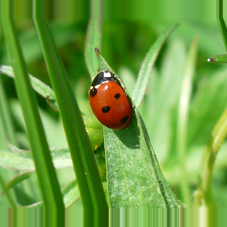
\includegraphics[height=2cm]{data/ladybug.png}
			};

			\newcommand{\outerarrow}{{Latex[length=0.2cm, width=0.3cm]}}
			\draw[-\outerarrow, line width=4pt, draw=gray] (input) to (n00);

			\node[] at ($ (n30) + (0, \vsep+0.75*\nodesize) $) {Konvolusjonelt nevralt nettverk};
		\end{tikzpicture}
	\end{frame}

	% XAI: First layer
	\begin{frame}{Forklarbar AI: Layerwise relevance propagation}
		\begin{tikzpicture}
			\newcommand{\nodesize}{8pt}
			\newcommand{\hsep}{24pt}
			\newcommand{\vsep}{12pt}

			\newcommand{\arrowwidth}{0.05cm}
			\newcommand{\innerarrow}{{Latex[length=0.1cm, width=0.15cm]}}

			\newcommand{\modellocation}[1]{($ (0, 0) + ####1 $)}

			\node[circle, inner sep=0pt, fill=none, outer sep=0pt, line width=0pt, draw=none] (n00) at \modellocation{(-3 * \hsep, 0)} {};
			\node[] at (-5.5, 1.5) {};
			\node[] at (5.1, -1.2) {};

			\draw[black, fill=gray!20] (n00.center) --
							($ (n00) + (0, 2*\vsep+0.5*\nodesize+2pt) $) --
							($ (n00) + (6*\hsep+0.5*\nodesize+2pt, 2*\vsep+0.5*\nodesize+2pt) $) --
							($ (n00) + (6*\hsep+0.5*\nodesize+2pt, -2*\vsep-0.5*\nodesize-2pt) $) --
							($ (n00) + (0, -2*\vsep-0.5*\nodesize-2pt) $) --
							(n00.center);


			\node[circle, draw=black, minimum size=\nodesize, inner sep=0pt, fill=train-fill!35, outer sep=0pt, line width=0pt, draw=train-fill!35] (n10) at \modellocation{(-2 * \hsep, 2 * \vsep)} {};
			\node[circle, minimum size=\nodesize, inner sep=0pt, fill=train-fill, outer sep=0pt, line width=0pt, draw=train-fill] (n11) at \modellocation{(-2 * \hsep, 1 * \vsep)} {};
			\node[circle, minimum size=\nodesize, inner sep=0pt, fill=train-fill!15, outer sep=0pt, line width=0pt, draw=train-fill!15] (n12) at \modellocation{(-2 * \hsep, 0)} {};
			\node[circle, minimum size=\nodesize, inner sep=0pt, fill=train-fill!85, outer sep=0pt, line width=0pt, draw=train-fill!85] (n13) at \modellocation{(-2 * \hsep, -1 * \vsep)} {};
			\node[circle, minimum size=\nodesize, inner sep=0pt, fill=train-fill!90, outer sep=0pt, line width=0pt, draw=train-fill!90] (n14) at \modellocation{(-2 * \hsep, -2 * \vsep)} {};

			\node[circle, minimum size=\nodesize, inner sep=0pt, fill=gray, outer sep=0pt, line width=0pt, draw=gray] (n20) at \modellocation{(-1 * \hsep, 1.5 * \vsep)} {};
			\node[circle, minimum size=\nodesize, inner sep=0pt, fill=gray, outer sep=0pt, line width=0pt, draw=gray] (n21) at \modellocation{(-1 * \hsep, 0.5 * \vsep)} {};
			\node[circle, minimum size=\nodesize, inner sep=0pt, fill=gray, outer sep=0pt, line width=0pt, draw=gray] (n22) at \modellocation{(-1 * \hsep, -0.5 * \vsep)} {};
			\node[circle, minimum size=\nodesize, inner sep=0pt, fill=gray, outer sep=0pt, line width=0pt, draw=gray] (n23) at \modellocation{(-1 * \hsep, -1.5 * \vsep)} {};

			\node[circle, minimum size=\nodesize, inner sep=0pt, fill=gray, outer sep=0pt, line width=0pt, draw=gray] (n30) at \modellocation{(0 * \hsep, 1.5 * \vsep)} {};
			\node[circle, minimum size=\nodesize, inner sep=0pt, fill=gray, outer sep=0pt, line width=0pt, draw=gray] (n31) at \modellocation{(0 * \hsep, 0.5 * \vsep)} {};
			\node[circle, minimum size=\nodesize, inner sep=0pt, fill=gray, outer sep=0pt, line width=0pt, draw=gray] (n32) at \modellocation{(0 * \hsep, -0.5 * \vsep)} {};
			\node[circle, minimum size=\nodesize, inner sep=0pt, fill=gray, outer sep=0pt, line width=0pt, draw=gray] (n33) at \modellocation{(0 * \hsep, -1.5 * \vsep)} {};

			\node[circle, minimum size=\nodesize, inner sep=0pt, fill=gray, outer sep=0pt, line width=0pt, draw=gray] (n40) at \modellocation{(1 * \hsep, 1*\vsep)} {};
			\node[circle, minimum size=\nodesize, inner sep=0pt, fill=gray, outer sep=0pt, line width=0pt, draw=gray] (n41) at \modellocation{(1 * \hsep, 0*\vsep)} {};
			\node[circle, minimum size=\nodesize, inner sep=0pt, fill=gray, outer sep=0pt, line width=0pt, draw=gray] (n42) at \modellocation{(1 * \hsep, -1*\vsep)} {};

			\node[circle, minimum size=\nodesize, inner sep=0pt, fill=gray, outer sep=0pt, line width=0pt, draw=gray] (n50) at \modellocation{(2 * \hsep, 1*\vsep)} {};
			\node[circle, minimum size=\nodesize, inner sep=0pt, fill=gray, outer sep=0pt, line width=0pt, draw=gray] (n51) at \modellocation{(2 * \hsep, 0*\vsep)} {};
			\node[circle, minimum size=\nodesize, inner sep=0pt, fill=gray, outer sep=0pt, line width=0pt, draw=gray] (n52) at \modellocation{(2 * \hsep, -1*\vsep)} {};

			\node[circle, minimum size=\nodesize, inner sep=0pt, fill=gray, outer sep=0pt, line width=0pt, draw=gray] (n60) at \modellocation{(3 * \hsep, 0)} {};

			\draw[
				color=train-fill!35,
				-\innerarrow,
				line width=\arrowwidth
			] (n00) to [out=20,in=200] (n10) {};
			\draw[
				color=train-fill,
				-\innerarrow,
				line width=\arrowwidth
			] (n00) to [out=10,in=190] (n11) {};
			\draw[
				color=train-fill!15,
				-\innerarrow,
				line width=\arrowwidth
			] (n00) to [out=0,in=180] (n12) {};
			\draw[
				color=train-fill!85,
				-\innerarrow,
				line width=\arrowwidth
			] (n00) to [out=-10,in=170] (n13) {};
			\draw[
				color=train-fill!90,
				-\innerarrow,
				line width=\arrowwidth
			] (n00) to [out=-20,in=160] (n14) {};

			\draw[
				color=gray!70,
				-\innerarrow,
				line width=\arrowwidth
			] (n10) to [out=-5,in=175] (n20) {};
			\draw[
				color=gray!70,
				-\innerarrow,
				line width=\arrowwidth
			] (n10) to [out=-15,in=165] (n21) {};
			\draw[
				color=gray!70,
				-\innerarrow,
				line width=\arrowwidth
			] (n10) to [out=-25,in=155] (n22) {};
			\draw[
				color=gray!70,
				-\innerarrow,
				line width=\arrowwidth
			] (n10) to [out=-35,in=145] (n23) {};

			\draw[
				color=gray!70,
				-\innerarrow,
				line width=\arrowwidth
			] (n11) to [out=5,in=185] (n20) {};
			\draw[
				color=gray!70,
				-\innerarrow,
				line width=\arrowwidth
			] (n11) to [out=-5,in=175] (n21) {};
			\draw[
				color=gray!70,
				-\innerarrow,
				line width=\arrowwidth
			] (n11) to [out=-15,in=165] (n22) {};
			\draw[
				color=gray!70,
				-\innerarrow,
				line width=\arrowwidth
			] (n11) to [out=-25,in=155] (n23) {};

			\draw[
				color=gray!70,
				-\innerarrow,
				line width=\arrowwidth
			] (n12) to [out=15,in=195] (n20) {};
			\draw[
				color=gray!70,
				-\innerarrow,
				line width=\arrowwidth
			] (n12) to [out=5,in=185] (n21) {};
			\draw[
				color=gray!70,
				-\innerarrow,
				line width=\arrowwidth
			] (n12) to [out=-5,in=175] (n22) {};
			\draw[
				color=gray!70,
				-\innerarrow,
				line width=\arrowwidth
			] (n12) to [out=-15,in=165] (n23) {};

			\draw[
				color=gray!70,
				-\innerarrow,
				line width=\arrowwidth
			] (n13) to [out=25,in=205] (n20) {};
			\draw[
				color=gray!70,
				-\innerarrow,
				line width=\arrowwidth
			] (n13) to [out=15,in=195] (n21) {};
			\draw[
				color=gray!70,
				-\innerarrow,
				line width=\arrowwidth
			] (n13) to [out=5,in=185] (n22) {};
			\draw[
				color=gray!70,
				-\innerarrow,
				line width=\arrowwidth
			] (n13) to [out=-5,in=175] (n23) {};

			\draw[
				color=gray!70,
				-\innerarrow,
				line width=\arrowwidth
			] (n14) to [out=35,in=215] (n20) {};
			\draw[
				color=gray!70,
				-\innerarrow,
				line width=\arrowwidth
			] (n14) to [out=25,in=205] (n21) {};
			\draw[
				color=gray!70,
				-\innerarrow,
				line width=\arrowwidth
			] (n14) to [out=15,in=195] (n22) {};
			\draw[
				color=gray!70,
				-\innerarrow,
				line width=\arrowwidth
			] (n14) to [out=5,in=185] (n23) {};

			\draw[
				color=gray!70,
				-\innerarrow,
				line width=\arrowwidth
			] (n20) to [out=0,in=180] (n30) {};
			\draw[
				color=gray!70,
				-\innerarrow,
				line width=\arrowwidth
			] (n20) to [out=-10,in=170] (n31) {};
			\draw[
				color=gray!70,
				-\innerarrow,
				line width=\arrowwidth
			] (n20) to [out=-20,in=160] (n32) {};
			\draw[
				color=gray!70,
				-\innerarrow,
				line width=\arrowwidth
			] (n20) to [out=-30,in=150] (n33) {};

			\draw[
				color=gray!70,
				-\innerarrow,
				line width=\arrowwidth
			] (n21) to [out=10,in=190] (n30) {};
			\draw[
				color=gray!70,
				-\innerarrow,
				line width=\arrowwidth
			] (n21) to [out=0,in=180] (n31) {};
			\draw[
				color=gray!70,
				-\innerarrow,
				line width=\arrowwidth
			] (n21) to [out=-10,in=170] (n32) {};
			\draw[
				color=gray!70,
				-\innerarrow,
				line width=\arrowwidth
			] (n21) to [out=-20,in=160] (n33) {};

			\draw[
				color=gray!70,
				-\innerarrow,
				line width=\arrowwidth
			] (n22) to [out=20,in=200] (n30) {};
			\draw[
				color=gray!70,
				-\innerarrow,
				line width=\arrowwidth
			] (n22) to [out=10,in=190] (n31) {};
			\draw[
				color=gray!70,
				-\innerarrow,
				line width=\arrowwidth
			] (n22) to [out=0,in=180] (n32) {};
			\draw[
				color=gray!70,
				-\innerarrow,
				line width=\arrowwidth
			] (n22) to [out=-10,in=170] (n33) {};

			\draw[
				color=gray!70,
				-\innerarrow,
				line width=\arrowwidth
			] (n23) to [out=30,in=210] (n30) {};
			\draw[
				color=gray!70,
				-\innerarrow,
				line width=\arrowwidth
			] (n23) to [out=20,in=200] (n31) {};
			\draw[
				color=gray!70,
				-\innerarrow,
				line width=\arrowwidth
			] (n23) to [out=10,in=190] (n32) {};
			\draw[
				color=gray!70,
				-\innerarrow,
				line width=\arrowwidth
			] (n23) to [out=0,in=180] (n33) {};

			\draw[
				color=gray!70,
				-\innerarrow,
				line width=\arrowwidth
			] (n30) to [out=-5,in=175] (n40) {};
			\draw[
				color=gray!70,
				-\innerarrow,
				line width=\arrowwidth
			] (n30) to [out=-15,in=165] (n41) {};
			\draw[
				color=gray!70,
				-\innerarrow,
				line width=\arrowwidth
			] (n30) to [out=-25,in=155] (n42) {};

			\draw[
				color=gray!70,
				-\innerarrow,
				line width=\arrowwidth
			] (n31) to [out=5,in=185] (n40) {};
			\draw[
				color=gray!70,
				-\innerarrow,
				line width=\arrowwidth
			] (n31) to [out=-5,in=175] (n41) {};
			\draw[
				color=gray!70,
				-\innerarrow,
				line width=\arrowwidth
			] (n31) to [out=-15,in=165] (n42) {};

			\draw[
				color=gray!70,
				-\innerarrow,
				line width=\arrowwidth
			] (n32) to [out=15,in=195] (n40) {};
			\draw[
				color=gray!70,
				-\innerarrow,
				line width=\arrowwidth
			] (n32) to [out=5,in=185] (n41) {};
			\draw[
				color=gray!70,
				-\innerarrow,
				line width=\arrowwidth
			] (n32) to [out=-5,in=175] (n42) {};

			\draw[
				color=gray!70,
				-\innerarrow,
				line width=\arrowwidth
			] (n33) to [out=25,in=205] (n40) {};
			\draw[
				color=gray!70,
				-\innerarrow,
				line width=\arrowwidth
			] (n33) to [out=15,in=195] (n41) {};
			\draw[
				color=gray!70,
				-\innerarrow,
				line width=\arrowwidth
			] (n33) to [out=5,in=185] (n42) {};

			\draw[
				color=gray!70,
				-\innerarrow,
				line width=\arrowwidth
			] (n40) to [out=0,in=180] (n50) {};
			\draw[
				color=gray!70,
				-\innerarrow,
				line width=\arrowwidth
			] (n40) to [out=-10,in=170] (n51) {};
			\draw[
				color=gray!70,
				-\innerarrow,
				line width=\arrowwidth
			] (n40) to [out=-20,in=160] (n52) {};

			\draw[
				color=gray!70,
				-\innerarrow,
				line width=\arrowwidth
			] (n41) to [out=10,in=190] (n50) {};
			\draw[
				color=gray!70,
				-\innerarrow,
				line width=\arrowwidth
			] (n41) to [out=0,in=180] (n51) {};
			\draw[
				color=gray!70,
				-\innerarrow,
				line width=\arrowwidth
			] (n41) to [out=-10,in=170] (n52) {};

			\draw[
				color=gray!70,
				-\innerarrow,
				line width=\arrowwidth
			] (n42) to [out=20,in=200] (n50) {};
			\draw[
				color=gray!70,
				-\innerarrow,
				line width=\arrowwidth
			] (n42) to [out=10,in=190] (n51) {};
			\draw[
				color=gray!70,
				-\innerarrow,
				line width=\arrowwidth
			] (n42) to [out=0,in=180] (n52) {};

			\draw[
				color=gray!70,
				-\innerarrow,
				line width=\arrowwidth,
			] (n50) to [out=-10,in=170] (n60) {};
			\draw[
				color=gray!70,
				-\innerarrow,
				line width=\arrowwidth,
			] (n51) to [out=0,in=180] (n60) {};
			\draw[
				color=gray!70,
				-\innerarrow,
				line width=\arrowwidth,
			] (n52) to [out=10,in=190] (n60) {};


			\node[] at ($ (n30) + (0, \vsep+0.75*\nodesize) $) {Konvolusjonelt nevralt nettverk};

			\node[inner sep=0pt, outer sep=0pt, draw=black] (input) at ($ (n00) - (2, 0) $) {
				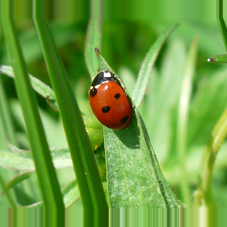
\includegraphics[height=2cm]{data/ladybug.png}
			};

			\newcommand{\outerarrow}{{Latex[length=0.2cm, width=0.3cm]}}
			\draw[-\outerarrow, line width=4pt, draw=gray] (input) to (n00);

		\end{tikzpicture}
	\end{frame}

	% XAI: Second layer
	\begin{frame}{Forklarbar AI: Layerwise relevance propagation}
		\begin{tikzpicture}
			\newcommand{\nodesize}{8pt}
			\newcommand{\hsep}{24pt}
			\newcommand{\vsep}{12pt}

			\newcommand{\arrowwidth}{0.05cm}
			\newcommand{\innerarrow}{{Latex[length=0.1cm, width=0.15cm]}}

			\newcommand{\modellocation}[1]{($ (0, 0) + ####1 $)}

			\node[circle, inner sep=0pt, fill=none, outer sep=0pt, line width=0pt, draw=none] (n00) at \modellocation{(-3 * \hsep, 0)} {};
			\node[] at (-5.5, 1.5) {};
			\node[] at (5.1, -1.2) {};

			\draw[black, fill=gray!20] (n00.center) --
							($ (n00) + (0, 2*\vsep+0.5*\nodesize+2pt) $) --
							($ (n00) + (6*\hsep+0.5*\nodesize+2pt, 2*\vsep+0.5*\nodesize+2pt) $) --
							($ (n00) + (6*\hsep+0.5*\nodesize+2pt, -2*\vsep-0.5*\nodesize-2pt) $) --
							($ (n00) + (0, -2*\vsep-0.5*\nodesize-2pt) $) --
							(n00.center);


			\node[circle, draw=black, minimum size=\nodesize, inner sep=0pt, fill=train-fill!35, outer sep=0pt, line width=0pt, draw=train-fill!35] (n10) at \modellocation{(-2 * \hsep, 2 * \vsep)} {};
			\node[circle, minimum size=\nodesize, inner sep=0pt, fill=train-fill, outer sep=0pt, line width=0pt, draw=train-fill] (n11) at \modellocation{(-2 * \hsep, 1 * \vsep)} {};
			\node[circle, minimum size=\nodesize, inner sep=0pt, fill=train-fill!15, outer sep=0pt, line width=0pt, draw=train-fill!15] (n12) at \modellocation{(-2 * \hsep, 0)} {};
			\node[circle, minimum size=\nodesize, inner sep=0pt, fill=train-fill!85, outer sep=0pt, line width=0pt, draw=train-fill!85] (n13) at \modellocation{(-2 * \hsep, -1 * \vsep)} {};
			\node[circle, minimum size=\nodesize, inner sep=0pt, fill=train-fill!90, outer sep=0pt, line width=0pt, draw=train-fill!90] (n14) at \modellocation{(-2 * \hsep, -2 * \vsep)} {};

			\node[circle, minimum size=\nodesize, inner sep=0pt, fill=train-fill!55, outer sep=0pt, line width=0pt, draw=train-fill!55] (n20) at \modellocation{(-1 * \hsep, 1.5 * \vsep)} {};
			\node[circle, minimum size=\nodesize, inner sep=0pt, fill=train-fill!20, outer sep=0pt, line width=0pt, draw=train-fill!20] (n21) at \modellocation{(-1 * \hsep, 0.5 * \vsep)} {};
			\node[circle, minimum size=\nodesize, inner sep=0pt, fill=train-fill!90, outer sep=0pt, line width=0pt, draw=train-fill!50] (n22) at \modellocation{(-1 * \hsep, -0.5 * \vsep)} {};
			\node[circle, minimum size=\nodesize, inner sep=0pt, fill=train-fill!35, outer sep=0pt, line width=0pt, draw=train-fill!35] (n23) at \modellocation{(-1 * \hsep, -1.5 * \vsep)} {};

			\node[circle, minimum size=\nodesize, inner sep=0pt, fill=gray, outer sep=0pt, line width=0pt, draw=gray] (n30) at \modellocation{(0 * \hsep, 1.5 * \vsep)} {};
			\node[circle, minimum size=\nodesize, inner sep=0pt, fill=gray, outer sep=0pt, line width=0pt, draw=gray] (n31) at \modellocation{(0 * \hsep, 0.5 * \vsep)} {};
			\node[circle, minimum size=\nodesize, inner sep=0pt, fill=gray, outer sep=0pt, line width=0pt, draw=gray] (n32) at \modellocation{(0 * \hsep, -0.5 * \vsep)} {};
			\node[circle, minimum size=\nodesize, inner sep=0pt, fill=gray, outer sep=0pt, line width=0pt, draw=gray] (n33) at \modellocation{(0 * \hsep, -1.5 * \vsep)} {};

			\node[circle, minimum size=\nodesize, inner sep=0pt, fill=gray, outer sep=0pt, line width=0pt, draw=gray] (n40) at \modellocation{(1 * \hsep, 1*\vsep)} {};
			\node[circle, minimum size=\nodesize, inner sep=0pt, fill=gray, outer sep=0pt, line width=0pt, draw=gray] (n41) at \modellocation{(1 * \hsep, 0*\vsep)} {};
			\node[circle, minimum size=\nodesize, inner sep=0pt, fill=gray, outer sep=0pt, line width=0pt, draw=gray] (n42) at \modellocation{(1 * \hsep, -1*\vsep)} {};

			\node[circle, minimum size=\nodesize, inner sep=0pt, fill=gray, outer sep=0pt, line width=0pt, draw=gray] (n50) at \modellocation{(2 * \hsep, 1*\vsep)} {};
			\node[circle, minimum size=\nodesize, inner sep=0pt, fill=gray, outer sep=0pt, line width=0pt, draw=gray] (n51) at \modellocation{(2 * \hsep, 0*\vsep)} {};
			\node[circle, minimum size=\nodesize, inner sep=0pt, fill=gray, outer sep=0pt, line width=0pt, draw=gray] (n52) at \modellocation{(2 * \hsep, -1*\vsep)} {};

			\node[circle, minimum size=\nodesize, inner sep=0pt, fill=gray, outer sep=0pt, line width=0pt, draw=gray] (n60) at \modellocation{(3 * \hsep, 0)} {};

			\draw[
				color=train-fill!35,
				-\innerarrow,
				line width=\arrowwidth
			] (n00) to [out=20,in=200] (n10) {};
			\draw[
				color=train-fill,
				-\innerarrow,
				line width=\arrowwidth
			] (n00) to [out=10,in=190] (n11) {};
			\draw[
				color=train-fill!15,
				-\innerarrow,
				line width=\arrowwidth
			] (n00) to [out=0,in=180] (n12) {};
			\draw[
				color=train-fill!85,
				-\innerarrow,
				line width=\arrowwidth
			] (n00) to [out=-10,in=170] (n13) {};
			\draw[
				color=train-fill!90,
				-\innerarrow,
				line width=\arrowwidth
			] (n00) to [out=-20,in=160] (n14) {};

			\draw[
				color=train-fill!35,
				-\innerarrow,
				line width=\arrowwidth
			] (n10) to [out=-5,in=175] (n20) {};
			\draw[
				color=train-fill!10,
				-\innerarrow,
				line width=\arrowwidth
			] (n10) to [out=-15,in=165] (n21) {};
			\draw[
				color=train-fill!70,
				-\innerarrow,
				line width=\arrowwidth
			] (n10) to [out=-25,in=155] (n22) {};
			\draw[
				color=train-fill!50,
				-\innerarrow,
				line width=\arrowwidth
			] (n10) to [out=-35,in=145] (n23) {};

			\draw[
				color=train-fill!30,
				-\innerarrow,
				line width=\arrowwidth
			] (n11) to [out=5,in=185] (n20) {};
			\draw[
				color=train-fill!25,
				-\innerarrow,
				line width=\arrowwidth
			] (n11) to [out=-5,in=175] (n21) {};
			\draw[
				color=train-fill!95,
				-\innerarrow,
				line width=\arrowwidth
			] (n11) to [out=-15,in=165] (n22) {};
			\draw[
				color=train-fill!35,
				-\innerarrow,
				line width=\arrowwidth
			] (n11) to [out=-25,in=155] (n23) {};

			\draw[
				color=train-fill!70,
				-\innerarrow,
				line width=\arrowwidth
			] (n12) to [out=15,in=195] (n20) {};
			\draw[
				color=train-fill!20,
				-\innerarrow,
				line width=\arrowwidth
			] (n12) to [out=5,in=185] (n21) {};
			\draw[
				color=train-fill!80,
				-\innerarrow,
				line width=\arrowwidth
			] (n12) to [out=-5,in=175] (n22) {};
			\draw[
				color=train-fill,
				-\innerarrow,
				line width=\arrowwidth
			] (n12) to [out=-15,in=165] (n23) {};

			\draw[
				color=train-fill!40,
				-\innerarrow,
				line width=\arrowwidth
			] (n13) to [out=25,in=205] (n20) {};
			\draw[
				color=train-fill!35,
				-\innerarrow,
				line width=\arrowwidth
			] (n13) to [out=15,in=195] (n21) {};
			\draw[
				color=train-fill!20,
				-\innerarrow,
				line width=\arrowwidth
			] (n13) to [out=5,in=185] (n22) {};
			\draw[
				color=white,
				-\innerarrow,
				line width=\arrowwidth
			] (n13) to [out=-5,in=175] (n23) {};

			\draw[
				color=train-fill!40,
				-\innerarrow,
				line width=\arrowwidth
			] (n14) to [out=35,in=215] (n20) {};
			\draw[
				color=train-fill!85,
				-\innerarrow,
				line width=\arrowwidth
			] (n14) to [out=25,in=205] (n21) {};
			\draw[
				color=train-fill!35,
				-\innerarrow,
				line width=\arrowwidth
			] (n14) to [out=15,in=195] (n22) {};
			\draw[
				color=train-fill,
				-\innerarrow,
				line width=\arrowwidth
			] (n14) to [out=5,in=185] (n23) {};

			\draw[
				color=gray!70,
				-\innerarrow,
				line width=\arrowwidth
			] (n20) to [out=0,in=180] (n30) {};
			\draw[
				color=gray!70,
				-\innerarrow,
				line width=\arrowwidth
			] (n20) to [out=-10,in=170] (n31) {};
			\draw[
				color=gray!70,
				-\innerarrow,
				line width=\arrowwidth
			] (n20) to [out=-20,in=160] (n32) {};
			\draw[
				color=gray!70,
				-\innerarrow,
				line width=\arrowwidth
			] (n20) to [out=-30,in=150] (n33) {};

			\draw[
				color=gray!70,
				-\innerarrow,
				line width=\arrowwidth
			] (n21) to [out=10,in=190] (n30) {};
			\draw[
				color=gray!70,
				-\innerarrow,
				line width=\arrowwidth
			] (n21) to [out=0,in=180] (n31) {};
			\draw[
				color=gray!70,
				-\innerarrow,
				line width=\arrowwidth
			] (n21) to [out=-10,in=170] (n32) {};
			\draw[
				color=gray!70,
				-\innerarrow,
				line width=\arrowwidth
			] (n21) to [out=-20,in=160] (n33) {};

			\draw[
				color=gray!70,
				-\innerarrow,
				line width=\arrowwidth
			] (n22) to [out=20,in=200] (n30) {};
			\draw[
				color=gray!70,
				-\innerarrow,
				line width=\arrowwidth
			] (n22) to [out=10,in=190] (n31) {};
			\draw[
				color=gray!70,
				-\innerarrow,
				line width=\arrowwidth
			] (n22) to [out=0,in=180] (n32) {};
			\draw[
				color=gray!70,
				-\innerarrow,
				line width=\arrowwidth
			] (n22) to [out=-10,in=170] (n33) {};

			\draw[
				color=gray!70,
				-\innerarrow,
				line width=\arrowwidth
			] (n23) to [out=30,in=210] (n30) {};
			\draw[
				color=gray!70,
				-\innerarrow,
				line width=\arrowwidth
			] (n23) to [out=20,in=200] (n31) {};
			\draw[
				color=gray!70,
				-\innerarrow,
				line width=\arrowwidth
			] (n23) to [out=10,in=190] (n32) {};
			\draw[
				color=gray!70,
				-\innerarrow,
				line width=\arrowwidth
			] (n23) to [out=0,in=180] (n33) {};

			\draw[
				color=gray!70,
				-\innerarrow,
				line width=\arrowwidth
			] (n30) to [out=-5,in=175] (n40) {};
			\draw[
				color=gray!70,
				-\innerarrow,
				line width=\arrowwidth
			] (n30) to [out=-15,in=165] (n41) {};
			\draw[
				color=gray!70,
				-\innerarrow,
				line width=\arrowwidth
			] (n30) to [out=-25,in=155] (n42) {};

			\draw[
				color=gray!70,
				-\innerarrow,
				line width=\arrowwidth
			] (n31) to [out=5,in=185] (n40) {};
			\draw[
				color=gray!70,
				-\innerarrow,
				line width=\arrowwidth
			] (n31) to [out=-5,in=175] (n41) {};
			\draw[
				color=gray!70,
				-\innerarrow,
				line width=\arrowwidth
			] (n31) to [out=-15,in=165] (n42) {};

			\draw[
				color=gray!70,
				-\innerarrow,
				line width=\arrowwidth
			] (n32) to [out=15,in=195] (n40) {};
			\draw[
				color=gray!70,
				-\innerarrow,
				line width=\arrowwidth
			] (n32) to [out=5,in=185] (n41) {};
			\draw[
				color=gray!70,
				-\innerarrow,
				line width=\arrowwidth
			] (n32) to [out=-5,in=175] (n42) {};

			\draw[
				color=gray!70,
				-\innerarrow,
				line width=\arrowwidth
			] (n33) to [out=25,in=205] (n40) {};
			\draw[
				color=gray!70,
				-\innerarrow,
				line width=\arrowwidth
			] (n33) to [out=15,in=195] (n41) {};
			\draw[
				color=gray!70,
				-\innerarrow,
				line width=\arrowwidth
			] (n33) to [out=5,in=185] (n42) {};

			\draw[
				color=gray!70,
				-\innerarrow,
				line width=\arrowwidth
			] (n40) to [out=0,in=180] (n50) {};
			\draw[
				color=gray!70,
				-\innerarrow,
				line width=\arrowwidth
			] (n40) to [out=-10,in=170] (n51) {};
			\draw[
				color=gray!70,
				-\innerarrow,
				line width=\arrowwidth
			] (n40) to [out=-20,in=160] (n52) {};

			\draw[
				color=gray!70,
				-\innerarrow,
				line width=\arrowwidth
			] (n41) to [out=10,in=190] (n50) {};
			\draw[
				color=gray!70,
				-\innerarrow,
				line width=\arrowwidth
			] (n41) to [out=0,in=180] (n51) {};
			\draw[
				color=gray!70,
				-\innerarrow,
				line width=\arrowwidth
			] (n41) to [out=-10,in=170] (n52) {};

			\draw[
				color=gray!70,
				-\innerarrow,
				line width=\arrowwidth
			] (n42) to [out=20,in=200] (n50) {};
			\draw[
				color=gray!70,
				-\innerarrow,
				line width=\arrowwidth
			] (n42) to [out=10,in=190] (n51) {};
			\draw[
				color=gray!70,
				-\innerarrow,
				line width=\arrowwidth
			] (n42) to [out=0,in=180] (n52) {};

			\draw[
				color=gray!70,
				-\innerarrow,
				line width=\arrowwidth,
			] (n50) to [out=-10,in=170] (n60) {};
			\draw[
				color=gray!70,
				-\innerarrow,
				line width=\arrowwidth,
			] (n51) to [out=0,in=180] (n60) {};
			\draw[
				color=gray!70,
				-\innerarrow,
				line width=\arrowwidth,
			] (n52) to [out=10,in=190] (n60) {};


			\node[] at ($ (n30) + (0, \vsep+0.75*\nodesize) $) {Konvolusjonelt nevralt nettverk};

			\node[inner sep=0pt, outer sep=0pt, draw=black] (input) at ($ (n00) - (2, 0) $) {
				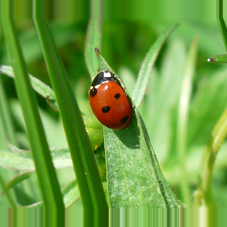
\includegraphics[height=2cm]{data/ladybug.png}
			};

			\newcommand{\outerarrow}{{Latex[length=0.2cm, width=0.3cm]}}
			\draw[-\outerarrow, line width=4pt, draw=gray] (input) to (n00);

		\end{tikzpicture}
	\end{frame}

	% XAI: Third layer
	\begin{frame}{Forklarbar AI: Layerwise relevance propagation}
		\begin{tikzpicture}
			\newcommand{\nodesize}{8pt}
			\newcommand{\hsep}{24pt}
			\newcommand{\vsep}{12pt}

			\newcommand{\arrowwidth}{0.05cm}
			\newcommand{\innerarrow}{{Latex[length=0.1cm, width=0.15cm]}}

			\newcommand{\modellocation}[1]{($ (0, 0) + ####1 $)}

			\node[circle, inner sep=0pt, fill=none, outer sep=0pt, line width=0pt, draw=none] (n00) at \modellocation{(-3 * \hsep, 0)} {};
			\node[] at (-5.5, 1.5) {};
			\node[] at (5.1, -1.2) {};

			\draw[black, fill=gray!20] (n00.center) --
							($ (n00) + (0, 2*\vsep+0.5*\nodesize+2pt) $) --
							($ (n00) + (6*\hsep+0.5*\nodesize+2pt, 2*\vsep+0.5*\nodesize+2pt) $) --
							($ (n00) + (6*\hsep+0.5*\nodesize+2pt, -2*\vsep-0.5*\nodesize-2pt) $) --
							($ (n00) + (0, -2*\vsep-0.5*\nodesize-2pt) $) --
							(n00.center);


			\node[circle, draw=black, minimum size=\nodesize, inner sep=0pt, fill=train-fill!35, outer sep=0pt, line width=0pt, draw=train-fill!35] (n10) at \modellocation{(-2 * \hsep, 2 * \vsep)} {};
			\node[circle, minimum size=\nodesize, inner sep=0pt, fill=train-fill, outer sep=0pt, line width=0pt, draw=train-fill] (n11) at \modellocation{(-2 * \hsep, 1 * \vsep)} {};
			\node[circle, minimum size=\nodesize, inner sep=0pt, fill=train-fill!15, outer sep=0pt, line width=0pt, draw=train-fill!15] (n12) at \modellocation{(-2 * \hsep, 0)} {};
			\node[circle, minimum size=\nodesize, inner sep=0pt, fill=train-fill!85, outer sep=0pt, line width=0pt, draw=train-fill!85] (n13) at \modellocation{(-2 * \hsep, -1 * \vsep)} {};
			\node[circle, minimum size=\nodesize, inner sep=0pt, fill=train-fill!90, outer sep=0pt, line width=0pt, draw=train-fill!90] (n14) at \modellocation{(-2 * \hsep, -2 * \vsep)} {};

			\node[circle, minimum size=\nodesize, inner sep=0pt, fill=train-fill!55, outer sep=0pt, line width=0pt, draw=train-fill!55] (n20) at \modellocation{(-1 * \hsep, 1.5 * \vsep)} {};
			\node[circle, minimum size=\nodesize, inner sep=0pt, fill=train-fill!20, outer sep=0pt, line width=0pt, draw=train-fill!20] (n21) at \modellocation{(-1 * \hsep, 0.5 * \vsep)} {};
			\node[circle, minimum size=\nodesize, inner sep=0pt, fill=train-fill!90, outer sep=0pt, line width=0pt, draw=train-fill!50] (n22) at \modellocation{(-1 * \hsep, -0.5 * \vsep)} {};
			\node[circle, minimum size=\nodesize, inner sep=0pt, fill=train-fill!35, outer sep=0pt, line width=0pt, draw=train-fill!35] (n23) at \modellocation{(-1 * \hsep, -1.5 * \vsep)} {};

			\node[circle, minimum size=\nodesize, inner sep=0pt, fill=train-fill!95, outer sep=0pt, line width=0pt, draw=train-fill!65] (n30) at \modellocation{(0 * \hsep, 1.5 * \vsep)} {};
			\node[circle, minimum size=\nodesize, inner sep=0pt, fill=train-fill!20, outer sep=0pt, line width=0pt, draw=train-fill!20] (n31) at \modellocation{(0 * \hsep, 0.5 * \vsep)} {};
			\node[circle, minimum size=\nodesize, inner sep=0pt, fill=train-fill!90, outer sep=0pt, line width=0pt, draw=train-fill!90] (n32) at \modellocation{(0 * \hsep, -0.5 * \vsep)} {};
			\node[circle, minimum size=\nodesize, inner sep=0pt, fill=train-fill!80, outer sep=0pt, line width=0pt, draw=train-fill!80] (n33) at \modellocation{(0 * \hsep, -1.5 * \vsep)} {};

			\node[circle, minimum size=\nodesize, inner sep=0pt, fill=gray, outer sep=0pt, line width=0pt, draw=gray] (n40) at \modellocation{(1 * \hsep, 1*\vsep)} {};
			\node[circle, minimum size=\nodesize, inner sep=0pt, fill=gray, outer sep=0pt, line width=0pt, draw=gray] (n41) at \modellocation{(1 * \hsep, 0*\vsep)} {};
			\node[circle, minimum size=\nodesize, inner sep=0pt, fill=gray, outer sep=0pt, line width=0pt, draw=gray] (n42) at \modellocation{(1 * \hsep, -1*\vsep)} {};

			\node[circle, minimum size=\nodesize, inner sep=0pt, fill=gray, outer sep=0pt, line width=0pt, draw=gray] (n50) at \modellocation{(2 * \hsep, 1*\vsep)} {};
			\node[circle, minimum size=\nodesize, inner sep=0pt, fill=gray, outer sep=0pt, line width=0pt, draw=gray] (n51) at \modellocation{(2 * \hsep, 0*\vsep)} {};
			\node[circle, minimum size=\nodesize, inner sep=0pt, fill=gray, outer sep=0pt, line width=0pt, draw=gray] (n52) at \modellocation{(2 * \hsep, -1*\vsep)} {};

			\node[circle, minimum size=\nodesize, inner sep=0pt, fill=gray, outer sep=0pt, line width=0pt, draw=gray] (n60) at \modellocation{(3 * \hsep, 0)} {};

			\draw[
				color=train-fill!35,
				-\innerarrow,
				line width=\arrowwidth
			] (n00) to [out=20,in=200] (n10) {};
			\draw[
				color=train-fill,
				-\innerarrow,
				line width=\arrowwidth
			] (n00) to [out=10,in=190] (n11) {};
			\draw[
				color=train-fill!15,
				-\innerarrow,
				line width=\arrowwidth
			] (n00) to [out=0,in=180] (n12) {};
			\draw[
				color=train-fill!85,
				-\innerarrow,
				line width=\arrowwidth
			] (n00) to [out=-10,in=170] (n13) {};
			\draw[
				color=train-fill!90,
				-\innerarrow,
				line width=\arrowwidth
			] (n00) to [out=-20,in=160] (n14) {};

			\draw[
				color=train-fill!35,
				-\innerarrow,
				line width=\arrowwidth
			] (n10) to [out=-5,in=175] (n20) {};
			\draw[
				color=train-fill!10,
				-\innerarrow,
				line width=\arrowwidth
			] (n10) to [out=-15,in=165] (n21) {};
			\draw[
				color=train-fill!70,
				-\innerarrow,
				line width=\arrowwidth
			] (n10) to [out=-25,in=155] (n22) {};
			\draw[
				color=train-fill!50,
				-\innerarrow,
				line width=\arrowwidth
			] (n10) to [out=-35,in=145] (n23) {};

			\draw[
				color=train-fill!30,
				-\innerarrow,
				line width=\arrowwidth
			] (n11) to [out=5,in=185] (n20) {};
			\draw[
				color=train-fill!25,
				-\innerarrow,
				line width=\arrowwidth
			] (n11) to [out=-5,in=175] (n21) {};
			\draw[
				color=train-fill!95,
				-\innerarrow,
				line width=\arrowwidth
			] (n11) to [out=-15,in=165] (n22) {};
			\draw[
				color=train-fill!35,
				-\innerarrow,
				line width=\arrowwidth
			] (n11) to [out=-25,in=155] (n23) {};

			\draw[
				color=train-fill!70,
				-\innerarrow,
				line width=\arrowwidth
			] (n12) to [out=15,in=195] (n20) {};
			\draw[
				color=train-fill!20,
				-\innerarrow,
				line width=\arrowwidth
			] (n12) to [out=5,in=185] (n21) {};
			\draw[
				color=train-fill!80,
				-\innerarrow,
				line width=\arrowwidth
			] (n12) to [out=-5,in=175] (n22) {};
			\draw[
				color=train-fill,
				-\innerarrow,
				line width=\arrowwidth
			] (n12) to [out=-15,in=165] (n23) {};

			\draw[
				color=train-fill!40,
				-\innerarrow,
				line width=\arrowwidth
			] (n13) to [out=25,in=205] (n20) {};
			\draw[
				color=train-fill!35,
				-\innerarrow,
				line width=\arrowwidth
			] (n13) to [out=15,in=195] (n21) {};
			\draw[
				color=train-fill!20,
				-\innerarrow,
				line width=\arrowwidth
			] (n13) to [out=5,in=185] (n22) {};
			\draw[
				color=white,
				-\innerarrow,
				line width=\arrowwidth
			] (n13) to [out=-5,in=175] (n23) {};

			\draw[
				color=train-fill!40,
				-\innerarrow,
				line width=\arrowwidth
			] (n14) to [out=35,in=215] (n20) {};
			\draw[
				color=train-fill!85,
				-\innerarrow,
				line width=\arrowwidth
			] (n14) to [out=25,in=205] (n21) {};
			\draw[
				color=train-fill!35,
				-\innerarrow,
				line width=\arrowwidth
			] (n14) to [out=15,in=195] (n22) {};
			\draw[
				color=train-fill,
				-\innerarrow,
				line width=\arrowwidth
			] (n14) to [out=5,in=185] (n23) {};

			\draw[
				color=train-fill!85,
				-\innerarrow,
				line width=\arrowwidth
			] (n20) to [out=0,in=180] (n30) {};
			\draw[
				color=train-fill!50,
				-\innerarrow,
				line width=\arrowwidth
			] (n20) to [out=-10,in=170] (n31) {};
			\draw[
				color=train-fill!75,
				-\innerarrow,
				line width=\arrowwidth
			] (n20) to [out=-20,in=160] (n32) {};
			\draw[
				color=white,
				-\innerarrow,
				line width=\arrowwidth
			] (n20) to [out=-30,in=150] (n33) {};

			\draw[
				color=train-fill,
				-\innerarrow,
				line width=\arrowwidth
			] (n21) to [out=10,in=190] (n30) {};
			\draw[
				color=train-fill!30,
				-\innerarrow,
				line width=\arrowwidth
			] (n21) to [out=0,in=180] (n31) {};
			\draw[
				color=train-fill!25,
				-\innerarrow,
				line width=\arrowwidth
			] (n21) to [out=-10,in=170] (n32) {};
			\draw[
				color=white,
				-\innerarrow,
				line width=\arrowwidth
			] (n21) to [out=-20,in=160] (n33) {};

			\draw[
				color=train-fill!35,
				-\innerarrow,
				line width=\arrowwidth
			] (n22) to [out=20,in=200] (n30) {};
			\draw[
				color=train-fill!95,
				-\innerarrow,
				line width=\arrowwidth
			] (n22) to [out=10,in=190] (n31) {};
			\draw[
				color=train-fill!80,
				-\innerarrow,
				line width=\arrowwidth
			] (n22) to [out=0,in=180] (n32) {};
			\draw[
				color=white,
				-\innerarrow,
				line width=\arrowwidth
			] (n22) to [out=-10,in=170] (n33) {};

			\draw[
				color=train-fill!45,
				-\innerarrow,
				line width=\arrowwidth
			] (n23) to [out=30,in=210] (n30) {};
			\draw[
				color=train-fill!70,
				-\innerarrow,
				line width=\arrowwidth
			] (n23) to [out=20,in=200] (n31) {};
			\draw[
				color=train-fill!10,
				-\innerarrow,
				line width=\arrowwidth
			] (n23) to [out=10,in=190] (n32) {};
			\draw[
				color=train-fill!20,
				-\innerarrow,
				line width=\arrowwidth
			] (n23) to [out=0,in=180] (n33) {};

			\draw[
				color=gray!70,
				-\innerarrow,
				line width=\arrowwidth
			] (n30) to [out=-5,in=175] (n40) {};
			\draw[
				color=gray!70,
				-\innerarrow,
				line width=\arrowwidth
			] (n30) to [out=-15,in=165] (n41) {};
			\draw[
				color=gray!70,
				-\innerarrow,
				line width=\arrowwidth
			] (n30) to [out=-25,in=155] (n42) {};

			\draw[
				color=gray!70,
				-\innerarrow,
				line width=\arrowwidth
			] (n31) to [out=5,in=185] (n40) {};
			\draw[
				color=gray!70,
				-\innerarrow,
				line width=\arrowwidth
			] (n31) to [out=-5,in=175] (n41) {};
			\draw[
				color=gray!70,
				-\innerarrow,
				line width=\arrowwidth
			] (n31) to [out=-15,in=165] (n42) {};

			\draw[
				color=gray!70,
				-\innerarrow,
				line width=\arrowwidth
			] (n32) to [out=15,in=195] (n40) {};
			\draw[
				color=gray!70,
				-\innerarrow,
				line width=\arrowwidth
			] (n32) to [out=5,in=185] (n41) {};
			\draw[
				color=gray!70,
				-\innerarrow,
				line width=\arrowwidth
			] (n32) to [out=-5,in=175] (n42) {};

			\draw[
				color=gray!70,
				-\innerarrow,
				line width=\arrowwidth
			] (n33) to [out=25,in=205] (n40) {};
			\draw[
				color=gray!70,
				-\innerarrow,
				line width=\arrowwidth
			] (n33) to [out=15,in=195] (n41) {};
			\draw[
				color=gray!70,
				-\innerarrow,
				line width=\arrowwidth
			] (n33) to [out=5,in=185] (n42) {};

			\draw[
				color=gray!70,
				-\innerarrow,
				line width=\arrowwidth
			] (n40) to [out=0,in=180] (n50) {};
			\draw[
				color=gray!70,
				-\innerarrow,
				line width=\arrowwidth
			] (n40) to [out=-10,in=170] (n51) {};
			\draw[
				color=gray!70,
				-\innerarrow,
				line width=\arrowwidth
			] (n40) to [out=-20,in=160] (n52) {};

			\draw[
				color=gray!70,
				-\innerarrow,
				line width=\arrowwidth
			] (n41) to [out=10,in=190] (n50) {};
			\draw[
				color=gray!70,
				-\innerarrow,
				line width=\arrowwidth
			] (n41) to [out=0,in=180] (n51) {};
			\draw[
				color=gray!70,
				-\innerarrow,
				line width=\arrowwidth
			] (n41) to [out=-10,in=170] (n52) {};

			\draw[
				color=gray!70,
				-\innerarrow,
				line width=\arrowwidth
			] (n42) to [out=20,in=200] (n50) {};
			\draw[
				color=gray!70,
				-\innerarrow,
				line width=\arrowwidth
			] (n42) to [out=10,in=190] (n51) {};
			\draw[
				color=gray!70,
				-\innerarrow,
				line width=\arrowwidth
			] (n42) to [out=0,in=180] (n52) {};

			\draw[
				color=gray!70,
				-\innerarrow,
				line width=\arrowwidth,
			] (n50) to [out=-10,in=170] (n60) {};
			\draw[
				color=gray!70,
				-\innerarrow,
				line width=\arrowwidth,
			] (n51) to [out=0,in=180] (n60) {};
			\draw[
				color=gray!70,
				-\innerarrow,
				line width=\arrowwidth,
			] (n52) to [out=10,in=190] (n60) {};


			\node[] at ($ (n30) + (0, \vsep+0.75*\nodesize) $) {Konvolusjonelt nevralt nettverk};

			\node[inner sep=0pt, outer sep=0pt, draw=black] (input) at ($ (n00) - (2, 0) $) {
				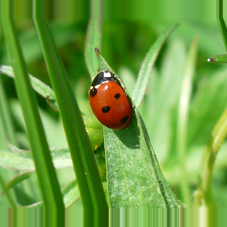
\includegraphics[height=2cm]{data/ladybug.png}
			};

			\newcommand{\outerarrow}{{Latex[length=0.2cm, width=0.3cm]}}
			\draw[-\outerarrow, line width=4pt, draw=gray] (input) to (n00);

		\end{tikzpicture}
	\end{frame}

	% XAI: Fourth layer
	\begin{frame}{Forklarbar AI: Layerwise relevance propagation}
		\begin{tikzpicture}
			\newcommand{\nodesize}{8pt}
			\newcommand{\hsep}{24pt}
			\newcommand{\vsep}{12pt}

			\newcommand{\arrowwidth}{0.05cm}
			\newcommand{\innerarrow}{{Latex[length=0.1cm, width=0.15cm]}}

			\newcommand{\modellocation}[1]{($ (0, 0) + ####1 $)}

			\node[circle, inner sep=0pt, fill=none, outer sep=0pt, line width=0pt, draw=none] (n00) at \modellocation{(-3 * \hsep, 0)} {};
			\node[] at (-5.5, 1.5) {};
			\node[] at (5.1, -1.2) {};

			\draw[black, fill=gray!20] (n00.center) --
							($ (n00) + (0, 2*\vsep+0.5*\nodesize+2pt) $) --
							($ (n00) + (6*\hsep+0.5*\nodesize+2pt, 2*\vsep+0.5*\nodesize+2pt) $) --
							($ (n00) + (6*\hsep+0.5*\nodesize+2pt, -2*\vsep-0.5*\nodesize-2pt) $) --
							($ (n00) + (0, -2*\vsep-0.5*\nodesize-2pt) $) --
							(n00.center);


			\node[circle, draw=black, minimum size=\nodesize, inner sep=0pt, fill=train-fill!35, outer sep=0pt, line width=0pt, draw=train-fill!35] (n10) at \modellocation{(-2 * \hsep, 2 * \vsep)} {};
			\node[circle, minimum size=\nodesize, inner sep=0pt, fill=train-fill, outer sep=0pt, line width=0pt, draw=train-fill] (n11) at \modellocation{(-2 * \hsep, 1 * \vsep)} {};
			\node[circle, minimum size=\nodesize, inner sep=0pt, fill=train-fill!15, outer sep=0pt, line width=0pt, draw=train-fill!15] (n12) at \modellocation{(-2 * \hsep, 0)} {};
			\node[circle, minimum size=\nodesize, inner sep=0pt, fill=train-fill!85, outer sep=0pt, line width=0pt, draw=train-fill!85] (n13) at \modellocation{(-2 * \hsep, -1 * \vsep)} {};
			\node[circle, minimum size=\nodesize, inner sep=0pt, fill=train-fill!90, outer sep=0pt, line width=0pt, draw=train-fill!90] (n14) at \modellocation{(-2 * \hsep, -2 * \vsep)} {};

			\node[circle, minimum size=\nodesize, inner sep=0pt, fill=train-fill!55, outer sep=0pt, line width=0pt, draw=train-fill!55] (n20) at \modellocation{(-1 * \hsep, 1.5 * \vsep)} {};
			\node[circle, minimum size=\nodesize, inner sep=0pt, fill=train-fill!20, outer sep=0pt, line width=0pt, draw=train-fill!20] (n21) at \modellocation{(-1 * \hsep, 0.5 * \vsep)} {};
			\node[circle, minimum size=\nodesize, inner sep=0pt, fill=train-fill!90, outer sep=0pt, line width=0pt, draw=train-fill!50] (n22) at \modellocation{(-1 * \hsep, -0.5 * \vsep)} {};
			\node[circle, minimum size=\nodesize, inner sep=0pt, fill=train-fill!35, outer sep=0pt, line width=0pt, draw=train-fill!35] (n23) at \modellocation{(-1 * \hsep, -1.5 * \vsep)} {};

			\node[circle, minimum size=\nodesize, inner sep=0pt, fill=train-fill!95, outer sep=0pt, line width=0pt, draw=train-fill!65] (n30) at \modellocation{(0 * \hsep, 1.5 * \vsep)} {};
			\node[circle, minimum size=\nodesize, inner sep=0pt, fill=train-fill!20, outer sep=0pt, line width=0pt, draw=train-fill!20] (n31) at \modellocation{(0 * \hsep, 0.5 * \vsep)} {};
			\node[circle, minimum size=\nodesize, inner sep=0pt, fill=train-fill!90, outer sep=0pt, line width=0pt, draw=train-fill!90] (n32) at \modellocation{(0 * \hsep, -0.5 * \vsep)} {};
			\node[circle, minimum size=\nodesize, inner sep=0pt, fill=train-fill!80, outer sep=0pt, line width=0pt, draw=train-fill!80] (n33) at \modellocation{(0 * \hsep, -1.5 * \vsep)} {};

			\node[circle, minimum size=\nodesize, inner sep=0pt, fill=train-fill!50, outer sep=0pt, line width=0pt, draw=train-fill!50] (n40) at \modellocation{(1 * \hsep, 1*\vsep)} {};
			\node[circle, minimum size=\nodesize, inner sep=0pt, fill=train-fill!90, outer sep=0pt, line width=0pt, draw=train-fill!70] (n41) at \modellocation{(1 * \hsep, 0*\vsep)} {};
			\node[circle, minimum size=\nodesize, inner sep=0pt, fill=train-fill!70, outer sep=0pt, line width=0pt, draw=train-fill!30] (n42) at \modellocation{(1 * \hsep, -1*\vsep)} {};

			\node[circle, minimum size=\nodesize, inner sep=0pt, fill=gray, outer sep=0pt, line width=0pt, draw=gray] (n50) at \modellocation{(2 * \hsep, 1*\vsep)} {};
			\node[circle, minimum size=\nodesize, inner sep=0pt, fill=gray, outer sep=0pt, line width=0pt, draw=gray] (n51) at \modellocation{(2 * \hsep, 0*\vsep)} {};
			\node[circle, minimum size=\nodesize, inner sep=0pt, fill=gray, outer sep=0pt, line width=0pt, draw=gray] (n52) at \modellocation{(2 * \hsep, -1*\vsep)} {};

			\node[circle, minimum size=\nodesize, inner sep=0pt, fill=gray, outer sep=0pt, line width=0pt, draw=gray] (n60) at \modellocation{(3 * \hsep, 0)} {};

			\draw[
				color=train-fill!35,
				-\innerarrow,
				line width=\arrowwidth
			] (n00) to [out=20,in=200] (n10) {};
			\draw[
				color=train-fill,
				-\innerarrow,
				line width=\arrowwidth
			] (n00) to [out=10,in=190] (n11) {};
			\draw[
				color=train-fill!15,
				-\innerarrow,
				line width=\arrowwidth
			] (n00) to [out=0,in=180] (n12) {};
			\draw[
				color=train-fill!85,
				-\innerarrow,
				line width=\arrowwidth
			] (n00) to [out=-10,in=170] (n13) {};
			\draw[
				color=train-fill!90,
				-\innerarrow,
				line width=\arrowwidth
			] (n00) to [out=-20,in=160] (n14) {};

			\draw[
				color=train-fill!35,
				-\innerarrow,
				line width=\arrowwidth
			] (n10) to [out=-5,in=175] (n20) {};
			\draw[
				color=train-fill!10,
				-\innerarrow,
				line width=\arrowwidth
			] (n10) to [out=-15,in=165] (n21) {};
			\draw[
				color=train-fill!70,
				-\innerarrow,
				line width=\arrowwidth
			] (n10) to [out=-25,in=155] (n22) {};
			\draw[
				color=train-fill!50,
				-\innerarrow,
				line width=\arrowwidth
			] (n10) to [out=-35,in=145] (n23) {};

			\draw[
				color=train-fill!30,
				-\innerarrow,
				line width=\arrowwidth
			] (n11) to [out=5,in=185] (n20) {};
			\draw[
				color=train-fill!25,
				-\innerarrow,
				line width=\arrowwidth
			] (n11) to [out=-5,in=175] (n21) {};
			\draw[
				color=train-fill!95,
				-\innerarrow,
				line width=\arrowwidth
			] (n11) to [out=-15,in=165] (n22) {};
			\draw[
				color=train-fill!35,
				-\innerarrow,
				line width=\arrowwidth
			] (n11) to [out=-25,in=155] (n23) {};

			\draw[
				color=train-fill!70,
				-\innerarrow,
				line width=\arrowwidth
			] (n12) to [out=15,in=195] (n20) {};
			\draw[
				color=train-fill!20,
				-\innerarrow,
				line width=\arrowwidth
			] (n12) to [out=5,in=185] (n21) {};
			\draw[
				color=train-fill!80,
				-\innerarrow,
				line width=\arrowwidth
			] (n12) to [out=-5,in=175] (n22) {};
			\draw[
				color=train-fill,
				-\innerarrow,
				line width=\arrowwidth
			] (n12) to [out=-15,in=165] (n23) {};

			\draw[
				color=train-fill!40,
				-\innerarrow,
				line width=\arrowwidth
			] (n13) to [out=25,in=205] (n20) {};
			\draw[
				color=train-fill!35,
				-\innerarrow,
				line width=\arrowwidth
			] (n13) to [out=15,in=195] (n21) {};
			\draw[
				color=train-fill!20,
				-\innerarrow,
				line width=\arrowwidth
			] (n13) to [out=5,in=185] (n22) {};
			\draw[
				color=white,
				-\innerarrow,
				line width=\arrowwidth
			] (n13) to [out=-5,in=175] (n23) {};

			\draw[
				color=train-fill!40,
				-\innerarrow,
				line width=\arrowwidth
			] (n14) to [out=35,in=215] (n20) {};
			\draw[
				color=train-fill!85,
				-\innerarrow,
				line width=\arrowwidth
			] (n14) to [out=25,in=205] (n21) {};
			\draw[
				color=train-fill!35,
				-\innerarrow,
				line width=\arrowwidth
			] (n14) to [out=15,in=195] (n22) {};
			\draw[
				color=train-fill,
				-\innerarrow,
				line width=\arrowwidth
			] (n14) to [out=5,in=185] (n23) {};

			\draw[
				color=train-fill!85,
				-\innerarrow,
				line width=\arrowwidth
			] (n20) to [out=0,in=180] (n30) {};
			\draw[
				color=train-fill!50,
				-\innerarrow,
				line width=\arrowwidth
			] (n20) to [out=-10,in=170] (n31) {};
			\draw[
				color=train-fill!75,
				-\innerarrow,
				line width=\arrowwidth
			] (n20) to [out=-20,in=160] (n32) {};
			\draw[
				color=white,
				-\innerarrow,
				line width=\arrowwidth
			] (n20) to [out=-30,in=150] (n33) {};

			\draw[
				color=train-fill,
				-\innerarrow,
				line width=\arrowwidth
			] (n21) to [out=10,in=190] (n30) {};
			\draw[
				color=train-fill!30,
				-\innerarrow,
				line width=\arrowwidth
			] (n21) to [out=0,in=180] (n31) {};
			\draw[
				color=train-fill!25,
				-\innerarrow,
				line width=\arrowwidth
			] (n21) to [out=-10,in=170] (n32) {};
			\draw[
				color=white,
				-\innerarrow,
				line width=\arrowwidth
			] (n21) to [out=-20,in=160] (n33) {};

			\draw[
				color=train-fill!35,
				-\innerarrow,
				line width=\arrowwidth
			] (n22) to [out=20,in=200] (n30) {};
			\draw[
				color=train-fill!95,
				-\innerarrow,
				line width=\arrowwidth
			] (n22) to [out=10,in=190] (n31) {};
			\draw[
				color=train-fill!80,
				-\innerarrow,
				line width=\arrowwidth
			] (n22) to [out=0,in=180] (n32) {};
			\draw[
				color=white,
				-\innerarrow,
				line width=\arrowwidth
			] (n22) to [out=-10,in=170] (n33) {};

			\draw[
				color=train-fill!45,
				-\innerarrow,
				line width=\arrowwidth
			] (n23) to [out=30,in=210] (n30) {};
			\draw[
				color=train-fill!70,
				-\innerarrow,
				line width=\arrowwidth
			] (n23) to [out=20,in=200] (n31) {};
			\draw[
				color=train-fill!10,
				-\innerarrow,
				line width=\arrowwidth
			] (n23) to [out=10,in=190] (n32) {};
			\draw[
				color=train-fill!20,
				-\innerarrow,
				line width=\arrowwidth
			] (n23) to [out=0,in=180] (n33) {};

			\draw[
				color=train-fill!50,
				-\innerarrow,
				line width=\arrowwidth
			] (n30) to [out=-5,in=175] (n40) {};
			\draw[
				color=train-fill!30,
				-\innerarrow,
				line width=\arrowwidth
			] (n30) to [out=-15,in=165] (n41) {};
			\draw[
				color=train-fill,
				-\innerarrow,
				line width=\arrowwidth
			] (n30) to [out=-25,in=155] (n42) {};

			\draw[
				color=train-fill!45,
				-\innerarrow,
				line width=\arrowwidth
			] (n31) to [out=5,in=185] (n40) {};
			\draw[
				color=train-fill!90,
				-\innerarrow,
				line width=\arrowwidth
			] (n31) to [out=-5,in=175] (n41) {};
			\draw[
				color=train-fill!45,
				-\innerarrow,
				line width=\arrowwidth
			] (n31) to [out=-15,in=165] (n42) {};

			\draw[
				color=train-fill!15,
				-\innerarrow,
				line width=\arrowwidth
			] (n32) to [out=15,in=195] (n40) {};
			\draw[
				color=train-fill!70,
				-\innerarrow,
				line width=\arrowwidth
			] (n32) to [out=5,in=185] (n41) {};
			\draw[
				color=train-fill!50,
				-\innerarrow,
				line width=\arrowwidth
			] (n32) to [out=-5,in=175] (n42) {};

			\draw[
				color=train-fill!40,
				-\innerarrow,
				line width=\arrowwidth
			] (n33) to [out=25,in=205] (n40) {};
			\draw[
				color=train-fill!20,
				-\innerarrow,
				line width=\arrowwidth
			] (n33) to [out=15,in=195] (n41) {};
			\draw[
				color=train-fill!90,
				-\innerarrow,
				line width=\arrowwidth
			] (n33) to [out=5,in=185] (n42) {};

			\draw[
				color=gray!70,
				-\innerarrow,
				line width=\arrowwidth
			] (n40) to [out=0,in=180] (n50) {};
			\draw[
				color=gray!70,
				-\innerarrow,
				line width=\arrowwidth
			] (n40) to [out=-10,in=170] (n51) {};
			\draw[
				color=gray!70,
				-\innerarrow,
				line width=\arrowwidth
			] (n40) to [out=-20,in=160] (n52) {};

			\draw[
				color=gray!70,
				-\innerarrow,
				line width=\arrowwidth
			] (n41) to [out=10,in=190] (n50) {};
			\draw[
				color=gray!70,
				-\innerarrow,
				line width=\arrowwidth
			] (n41) to [out=0,in=180] (n51) {};
			\draw[
				color=gray!70,
				-\innerarrow,
				line width=\arrowwidth
			] (n41) to [out=-10,in=170] (n52) {};

			\draw[
				color=gray!70,
				-\innerarrow,
				line width=\arrowwidth
			] (n42) to [out=20,in=200] (n50) {};
			\draw[
				color=gray!70,
				-\innerarrow,
				line width=\arrowwidth
			] (n42) to [out=10,in=190] (n51) {};
			\draw[
				color=gray!70,
				-\innerarrow,
				line width=\arrowwidth
			] (n42) to [out=0,in=180] (n52) {};

			\draw[
				color=gray!70,
				-\innerarrow,
				line width=\arrowwidth,
			] (n50) to [out=-10,in=170] (n60) {};
			\draw[
				color=gray!70,
				-\innerarrow,
				line width=\arrowwidth,
			] (n51) to [out=0,in=180] (n60) {};
			\draw[
				color=gray!70,
				-\innerarrow,
				line width=\arrowwidth,
			] (n52) to [out=10,in=190] (n60) {};


			\node[] at ($ (n30) + (0, \vsep+0.75*\nodesize) $) {Konvolusjonelt nevralt nettverk};

			\node[inner sep=0pt, outer sep=0pt, draw=black] (input) at ($ (n00) - (2, 0) $) {
				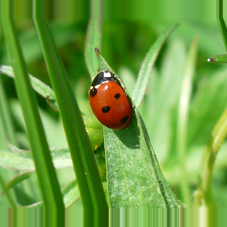
\includegraphics[height=2cm]{data/ladybug.png}
			};

			\newcommand{\outerarrow}{{Latex[length=0.2cm, width=0.3cm]}}
			\draw[-\outerarrow, line width=4pt, draw=gray] (input) to (n00);

		\end{tikzpicture}
	\end{frame}

	% XAI: Fifth layer
	\begin{frame}{Forklarbar AI: Layerwise relevance propagation}
		\begin{tikzpicture}
			\newcommand{\nodesize}{8pt}
			\newcommand{\hsep}{24pt}
			\newcommand{\vsep}{12pt}

			\newcommand{\arrowwidth}{0.05cm}
			\newcommand{\innerarrow}{{Latex[length=0.1cm, width=0.15cm]}}

			\newcommand{\modellocation}[1]{($ (0, 0) + ####1 $)}

			\node[circle, inner sep=0pt, fill=none, outer sep=0pt, line width=0pt, draw=none] (n00) at \modellocation{(-3 * \hsep, 0)} {};
			\node[] at (-5.5, 1.5) {};
			\node[] at (5.1, -1.2) {};

			\draw[black, fill=gray!20] (n00.center) --
							($ (n00) + (0, 2*\vsep+0.5*\nodesize+2pt) $) --
							($ (n00) + (6*\hsep+0.5*\nodesize+2pt, 2*\vsep+0.5*\nodesize+2pt) $) --
							($ (n00) + (6*\hsep+0.5*\nodesize+2pt, -2*\vsep-0.5*\nodesize-2pt) $) --
							($ (n00) + (0, -2*\vsep-0.5*\nodesize-2pt) $) --
							(n00.center);


			\node[circle, draw=black, minimum size=\nodesize, inner sep=0pt, fill=train-fill!35, outer sep=0pt, line width=0pt, draw=train-fill!35] (n10) at \modellocation{(-2 * \hsep, 2 * \vsep)} {};
			\node[circle, minimum size=\nodesize, inner sep=0pt, fill=train-fill, outer sep=0pt, line width=0pt, draw=train-fill] (n11) at \modellocation{(-2 * \hsep, 1 * \vsep)} {};
			\node[circle, minimum size=\nodesize, inner sep=0pt, fill=train-fill!15, outer sep=0pt, line width=0pt, draw=train-fill!15] (n12) at \modellocation{(-2 * \hsep, 0)} {};
			\node[circle, minimum size=\nodesize, inner sep=0pt, fill=train-fill!85, outer sep=0pt, line width=0pt, draw=train-fill!85] (n13) at \modellocation{(-2 * \hsep, -1 * \vsep)} {};
			\node[circle, minimum size=\nodesize, inner sep=0pt, fill=train-fill!90, outer sep=0pt, line width=0pt, draw=train-fill!90] (n14) at \modellocation{(-2 * \hsep, -2 * \vsep)} {};

			\node[circle, minimum size=\nodesize, inner sep=0pt, fill=train-fill!55, outer sep=0pt, line width=0pt, draw=train-fill!55] (n20) at \modellocation{(-1 * \hsep, 1.5 * \vsep)} {};
			\node[circle, minimum size=\nodesize, inner sep=0pt, fill=train-fill!20, outer sep=0pt, line width=0pt, draw=train-fill!20] (n21) at \modellocation{(-1 * \hsep, 0.5 * \vsep)} {};
			\node[circle, minimum size=\nodesize, inner sep=0pt, fill=train-fill!90, outer sep=0pt, line width=0pt, draw=train-fill!50] (n22) at \modellocation{(-1 * \hsep, -0.5 * \vsep)} {};
			\node[circle, minimum size=\nodesize, inner sep=0pt, fill=train-fill!35, outer sep=0pt, line width=0pt, draw=train-fill!35] (n23) at \modellocation{(-1 * \hsep, -1.5 * \vsep)} {};

			\node[circle, minimum size=\nodesize, inner sep=0pt, fill=train-fill!95, outer sep=0pt, line width=0pt, draw=train-fill!65] (n30) at \modellocation{(0 * \hsep, 1.5 * \vsep)} {};
			\node[circle, minimum size=\nodesize, inner sep=0pt, fill=train-fill!20, outer sep=0pt, line width=0pt, draw=train-fill!20] (n31) at \modellocation{(0 * \hsep, 0.5 * \vsep)} {};
			\node[circle, minimum size=\nodesize, inner sep=0pt, fill=train-fill!90, outer sep=0pt, line width=0pt, draw=train-fill!90] (n32) at \modellocation{(0 * \hsep, -0.5 * \vsep)} {};
			\node[circle, minimum size=\nodesize, inner sep=0pt, fill=train-fill!80, outer sep=0pt, line width=0pt, draw=train-fill!80] (n33) at \modellocation{(0 * \hsep, -1.5 * \vsep)} {};

			\node[circle, minimum size=\nodesize, inner sep=0pt, fill=train-fill!50, outer sep=0pt, line width=0pt, draw=train-fill!50] (n40) at \modellocation{(1 * \hsep, 1*\vsep)} {};
			\node[circle, minimum size=\nodesize, inner sep=0pt, fill=train-fill!90, outer sep=0pt, line width=0pt, draw=train-fill!70] (n41) at \modellocation{(1 * \hsep, 0*\vsep)} {};
			\node[circle, minimum size=\nodesize, inner sep=0pt, fill=train-fill!70, outer sep=0pt, line width=0pt, draw=train-fill!30] (n42) at \modellocation{(1 * \hsep, -1*\vsep)} {};

			\node[circle, minimum size=\nodesize, inner sep=0pt, fill=train-fill, outer sep=0pt, line width=0pt, draw=train-fill] (n50) at \modellocation{(2 * \hsep, 1*\vsep)} {};
			\node[circle, minimum size=\nodesize, inner sep=0pt, fill=train-fill!70, outer sep=0pt, line width=0pt, draw=train-fill!70] (n51) at \modellocation{(2 * \hsep, 0*\vsep)} {};
			\node[circle, minimum size=\nodesize, inner sep=0pt, fill=train-fill!30, outer sep=0pt, line width=0pt, draw=train-fill!30] (n52) at \modellocation{(2 * \hsep, -1*\vsep)} {};

			\node[circle, minimum size=\nodesize, inner sep=0pt, fill=gray, outer sep=0pt, line width=0pt, draw=gray] (n60) at \modellocation{(3 * \hsep, 0)} {};

			\draw[
				color=train-fill!35,
				-\innerarrow,
				line width=\arrowwidth
			] (n00) to [out=20,in=200] (n10) {};
			\draw[
				color=train-fill,
				-\innerarrow,
				line width=\arrowwidth
			] (n00) to [out=10,in=190] (n11) {};
			\draw[
				color=train-fill!15,
				-\innerarrow,
				line width=\arrowwidth
			] (n00) to [out=0,in=180] (n12) {};
			\draw[
				color=train-fill!85,
				-\innerarrow,
				line width=\arrowwidth
			] (n00) to [out=-10,in=170] (n13) {};
			\draw[
				color=train-fill!90,
				-\innerarrow,
				line width=\arrowwidth
			] (n00) to [out=-20,in=160] (n14) {};

			\draw[
				color=train-fill!35,
				-\innerarrow,
				line width=\arrowwidth
			] (n10) to [out=-5,in=175] (n20) {};
			\draw[
				color=train-fill!10,
				-\innerarrow,
				line width=\arrowwidth
			] (n10) to [out=-15,in=165] (n21) {};
			\draw[
				color=train-fill!70,
				-\innerarrow,
				line width=\arrowwidth
			] (n10) to [out=-25,in=155] (n22) {};
			\draw[
				color=train-fill!50,
				-\innerarrow,
				line width=\arrowwidth
			] (n10) to [out=-35,in=145] (n23) {};

			\draw[
				color=train-fill!30,
				-\innerarrow,
				line width=\arrowwidth
			] (n11) to [out=5,in=185] (n20) {};
			\draw[
				color=train-fill!25,
				-\innerarrow,
				line width=\arrowwidth
			] (n11) to [out=-5,in=175] (n21) {};
			\draw[
				color=train-fill!95,
				-\innerarrow,
				line width=\arrowwidth
			] (n11) to [out=-15,in=165] (n22) {};
			\draw[
				color=train-fill!35,
				-\innerarrow,
				line width=\arrowwidth
			] (n11) to [out=-25,in=155] (n23) {};

			\draw[
				color=train-fill!70,
				-\innerarrow,
				line width=\arrowwidth
			] (n12) to [out=15,in=195] (n20) {};
			\draw[
				color=train-fill!20,
				-\innerarrow,
				line width=\arrowwidth
			] (n12) to [out=5,in=185] (n21) {};
			\draw[
				color=train-fill!80,
				-\innerarrow,
				line width=\arrowwidth
			] (n12) to [out=-5,in=175] (n22) {};
			\draw[
				color=train-fill,
				-\innerarrow,
				line width=\arrowwidth
			] (n12) to [out=-15,in=165] (n23) {};

			\draw[
				color=train-fill!40,
				-\innerarrow,
				line width=\arrowwidth
			] (n13) to [out=25,in=205] (n20) {};
			\draw[
				color=train-fill!35,
				-\innerarrow,
				line width=\arrowwidth
			] (n13) to [out=15,in=195] (n21) {};
			\draw[
				color=train-fill!20,
				-\innerarrow,
				line width=\arrowwidth
			] (n13) to [out=5,in=185] (n22) {};
			\draw[
				color=white,
				-\innerarrow,
				line width=\arrowwidth
			] (n13) to [out=-5,in=175] (n23) {};

			\draw[
				color=train-fill!40,
				-\innerarrow,
				line width=\arrowwidth
			] (n14) to [out=35,in=215] (n20) {};
			\draw[
				color=train-fill!85,
				-\innerarrow,
				line width=\arrowwidth
			] (n14) to [out=25,in=205] (n21) {};
			\draw[
				color=train-fill!35,
				-\innerarrow,
				line width=\arrowwidth
			] (n14) to [out=15,in=195] (n22) {};
			\draw[
				color=train-fill,
				-\innerarrow,
				line width=\arrowwidth
			] (n14) to [out=5,in=185] (n23) {};

			\draw[
				color=train-fill!85,
				-\innerarrow,
				line width=\arrowwidth
			] (n20) to [out=0,in=180] (n30) {};
			\draw[
				color=train-fill!50,
				-\innerarrow,
				line width=\arrowwidth
			] (n20) to [out=-10,in=170] (n31) {};
			\draw[
				color=train-fill!75,
				-\innerarrow,
				line width=\arrowwidth
			] (n20) to [out=-20,in=160] (n32) {};
			\draw[
				color=white,
				-\innerarrow,
				line width=\arrowwidth
			] (n20) to [out=-30,in=150] (n33) {};

			\draw[
				color=train-fill,
				-\innerarrow,
				line width=\arrowwidth
			] (n21) to [out=10,in=190] (n30) {};
			\draw[
				color=train-fill!30,
				-\innerarrow,
				line width=\arrowwidth
			] (n21) to [out=0,in=180] (n31) {};
			\draw[
				color=train-fill!25,
				-\innerarrow,
				line width=\arrowwidth
			] (n21) to [out=-10,in=170] (n32) {};
			\draw[
				color=white,
				-\innerarrow,
				line width=\arrowwidth
			] (n21) to [out=-20,in=160] (n33) {};

			\draw[
				color=train-fill!35,
				-\innerarrow,
				line width=\arrowwidth
			] (n22) to [out=20,in=200] (n30) {};
			\draw[
				color=train-fill!95,
				-\innerarrow,
				line width=\arrowwidth
			] (n22) to [out=10,in=190] (n31) {};
			\draw[
				color=train-fill!80,
				-\innerarrow,
				line width=\arrowwidth
			] (n22) to [out=0,in=180] (n32) {};
			\draw[
				color=white,
				-\innerarrow,
				line width=\arrowwidth
			] (n22) to [out=-10,in=170] (n33) {};

			\draw[
				color=train-fill!45,
				-\innerarrow,
				line width=\arrowwidth
			] (n23) to [out=30,in=210] (n30) {};
			\draw[
				color=train-fill!70,
				-\innerarrow,
				line width=\arrowwidth
			] (n23) to [out=20,in=200] (n31) {};
			\draw[
				color=train-fill!10,
				-\innerarrow,
				line width=\arrowwidth
			] (n23) to [out=10,in=190] (n32) {};
			\draw[
				color=train-fill!20,
				-\innerarrow,
				line width=\arrowwidth
			] (n23) to [out=0,in=180] (n33) {};

			\draw[
				color=train-fill!50,
				-\innerarrow,
				line width=\arrowwidth
			] (n30) to [out=-5,in=175] (n40) {};
			\draw[
				color=train-fill!30,
				-\innerarrow,
				line width=\arrowwidth
			] (n30) to [out=-15,in=165] (n41) {};
			\draw[
				color=train-fill,
				-\innerarrow,
				line width=\arrowwidth
			] (n30) to [out=-25,in=155] (n42) {};

			\draw[
				color=train-fill!45,
				-\innerarrow,
				line width=\arrowwidth
			] (n31) to [out=5,in=185] (n40) {};
			\draw[
				color=train-fill!90,
				-\innerarrow,
				line width=\arrowwidth
			] (n31) to [out=-5,in=175] (n41) {};
			\draw[
				color=train-fill!45,
				-\innerarrow,
				line width=\arrowwidth
			] (n31) to [out=-15,in=165] (n42) {};

			\draw[
				color=train-fill!15,
				-\innerarrow,
				line width=\arrowwidth
			] (n32) to [out=15,in=195] (n40) {};
			\draw[
				color=train-fill!70,
				-\innerarrow,
				line width=\arrowwidth
			] (n32) to [out=5,in=185] (n41) {};
			\draw[
				color=train-fill!50,
				-\innerarrow,
				line width=\arrowwidth
			] (n32) to [out=-5,in=175] (n42) {};

			\draw[
				color=train-fill!40,
				-\innerarrow,
				line width=\arrowwidth
			] (n33) to [out=25,in=205] (n40) {};
			\draw[
				color=train-fill!20,
				-\innerarrow,
				line width=\arrowwidth
			] (n33) to [out=15,in=195] (n41) {};
			\draw[
				color=train-fill!90,
				-\innerarrow,
				line width=\arrowwidth
			] (n33) to [out=5,in=185] (n42) {};

			\draw[
				color=train-fill!25,
				-\innerarrow,
				line width=\arrowwidth
			] (n40) to [out=0,in=180] (n50) {};
			\draw[
				color=train-fill!15,
				-\innerarrow,
				line width=\arrowwidth
			] (n40) to [out=-10,in=170] (n51) {};
			\draw[
				color=train-fill,
				-\innerarrow,
				line width=\arrowwidth
			] (n40) to [out=-20,in=160] (n52) {};

			\draw[
				color=train-fill!35,
				-\innerarrow,
				line width=\arrowwidth
			] (n41) to [out=10,in=190] (n50) {};
			\draw[
				color=train-fill!10,
				-\innerarrow,
				line width=\arrowwidth
			] (n41) to [out=0,in=180] (n51) {};
			\draw[
				color=train-fill!90,
				-\innerarrow,
				line width=\arrowwidth
			] (n41) to [out=-10,in=170] (n52) {};

			\draw[
				color=train-fill!50,
				-\innerarrow,
				line width=\arrowwidth
			] (n42) to [out=20,in=200] (n50) {};
			\draw[
				color=train-fill!40,
				-\innerarrow,
				line width=\arrowwidth
			] (n42) to [out=10,in=190] (n51) {};
			\draw[
				color=train-fill!20,
				-\innerarrow,
				line width=\arrowwidth
			] (n42) to [out=0,in=180] (n52) {};

			\draw[
				color=gray!70,
				-\innerarrow,
				line width=\arrowwidth,
			] (n50) to [out=-10,in=170] (n60) {};
			\draw[
				color=gray!70,
				-\innerarrow,
				line width=\arrowwidth,
			] (n51) to [out=0,in=180] (n60) {};
			\draw[
				color=gray!70,
				-\innerarrow,
				line width=\arrowwidth,
			] (n52) to [out=10,in=190] (n60) {};


			\node[] at ($ (n30) + (0, \vsep+0.75*\nodesize) $) {Konvolusjonelt nevralt nettverk};

			\node[inner sep=0pt, outer sep=0pt, draw=black] (input) at ($ (n00) - (2, 0) $) {
				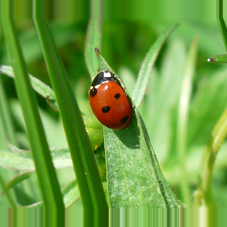
\includegraphics[height=2cm]{data/ladybug.png}
			};

			\newcommand{\outerarrow}{{Latex[length=0.2cm, width=0.3cm]}}
			\draw[-\outerarrow, line width=4pt, draw=gray] (input) to (n00);

		\end{tikzpicture}
	\end{frame}

	% XAI: Final layer
	\begin{frame}{Forklarbar AI: Layerwise relevance propagation}
		\begin{tikzpicture}
			\newcommand{\nodesize}{8pt}
			\newcommand{\hsep}{24pt}
			\newcommand{\vsep}{12pt}

			\newcommand{\arrowwidth}{0.05cm}
			\newcommand{\innerarrow}{{Latex[length=0.1cm, width=0.15cm]}}

			\newcommand{\modellocation}[1]{($ (0, 0) + ####1 $)}

			\node[circle, inner sep=0pt, fill=none, outer sep=0pt, line width=0pt, draw=none] (n00) at \modellocation{(-3 * \hsep, 0)} {};
			\node[] at (-5.5, 1.5) {};
			\node[] at (5.1, -1.2) {};

			\draw[black, fill=gray!20] (n00.center) --
							($ (n00) + (0, 2*\vsep+0.5*\nodesize+2pt) $) --
							($ (n00) + (6*\hsep+0.5*\nodesize+2pt, 2*\vsep+0.5*\nodesize+2pt) $) --
							($ (n00) + (6*\hsep+0.5*\nodesize+2pt, -2*\vsep-0.5*\nodesize-2pt) $) --
							($ (n00) + (0, -2*\vsep-0.5*\nodesize-2pt) $) --
							(n00.center);


			\node[circle, draw=black, minimum size=\nodesize, inner sep=0pt, fill=train-fill!35, outer sep=0pt, line width=0pt, draw=train-fill!35] (n10) at \modellocation{(-2 * \hsep, 2 * \vsep)} {};
			\node[circle, minimum size=\nodesize, inner sep=0pt, fill=train-fill, outer sep=0pt, line width=0pt, draw=train-fill] (n11) at \modellocation{(-2 * \hsep, 1 * \vsep)} {};
			\node[circle, minimum size=\nodesize, inner sep=0pt, fill=train-fill!15, outer sep=0pt, line width=0pt, draw=train-fill!15] (n12) at \modellocation{(-2 * \hsep, 0)} {};
			\node[circle, minimum size=\nodesize, inner sep=0pt, fill=train-fill!85, outer sep=0pt, line width=0pt, draw=train-fill!85] (n13) at \modellocation{(-2 * \hsep, -1 * \vsep)} {};
			\node[circle, minimum size=\nodesize, inner sep=0pt, fill=train-fill!90, outer sep=0pt, line width=0pt, draw=train-fill!90] (n14) at \modellocation{(-2 * \hsep, -2 * \vsep)} {};

			\node[circle, minimum size=\nodesize, inner sep=0pt, fill=train-fill!55, outer sep=0pt, line width=0pt, draw=train-fill!55] (n20) at \modellocation{(-1 * \hsep, 1.5 * \vsep)} {};
			\node[circle, minimum size=\nodesize, inner sep=0pt, fill=train-fill!20, outer sep=0pt, line width=0pt, draw=train-fill!20] (n21) at \modellocation{(-1 * \hsep, 0.5 * \vsep)} {};
			\node[circle, minimum size=\nodesize, inner sep=0pt, fill=train-fill!90, outer sep=0pt, line width=0pt, draw=train-fill!50] (n22) at \modellocation{(-1 * \hsep, -0.5 * \vsep)} {};
			\node[circle, minimum size=\nodesize, inner sep=0pt, fill=train-fill!35, outer sep=0pt, line width=0pt, draw=train-fill!35] (n23) at \modellocation{(-1 * \hsep, -1.5 * \vsep)} {};

			\node[circle, minimum size=\nodesize, inner sep=0pt, fill=train-fill!95, outer sep=0pt, line width=0pt, draw=train-fill!65] (n30) at \modellocation{(0 * \hsep, 1.5 * \vsep)} {};
			\node[circle, minimum size=\nodesize, inner sep=0pt, fill=train-fill!20, outer sep=0pt, line width=0pt, draw=train-fill!20] (n31) at \modellocation{(0 * \hsep, 0.5 * \vsep)} {};
			\node[circle, minimum size=\nodesize, inner sep=0pt, fill=train-fill!90, outer sep=0pt, line width=0pt, draw=train-fill!90] (n32) at \modellocation{(0 * \hsep, -0.5 * \vsep)} {};
			\node[circle, minimum size=\nodesize, inner sep=0pt, fill=train-fill!80, outer sep=0pt, line width=0pt, draw=train-fill!80] (n33) at \modellocation{(0 * \hsep, -1.5 * \vsep)} {};

			\node[circle, minimum size=\nodesize, inner sep=0pt, fill=train-fill!50, outer sep=0pt, line width=0pt, draw=train-fill!50] (n40) at \modellocation{(1 * \hsep, 1*\vsep)} {};
			\node[circle, minimum size=\nodesize, inner sep=0pt, fill=train-fill!90, outer sep=0pt, line width=0pt, draw=train-fill!70] (n41) at \modellocation{(1 * \hsep, 0*\vsep)} {};
			\node[circle, minimum size=\nodesize, inner sep=0pt, fill=train-fill!70, outer sep=0pt, line width=0pt, draw=train-fill!30] (n42) at \modellocation{(1 * \hsep, -1*\vsep)} {};

			\node[circle, minimum size=\nodesize, inner sep=0pt, fill=train-fill, outer sep=0pt, line width=0pt, draw=train-fill] (n50) at \modellocation{(2 * \hsep, 1*\vsep)} {};
			\node[circle, minimum size=\nodesize, inner sep=0pt, fill=train-fill!70, outer sep=0pt, line width=0pt, draw=train-fill!70] (n51) at \modellocation{(2 * \hsep, 0*\vsep)} {};
			\node[circle, minimum size=\nodesize, inner sep=0pt, fill=train-fill!30, outer sep=0pt, line width=0pt, draw=train-fill!30] (n52) at \modellocation{(2 * \hsep, -1*\vsep)} {};

			\node[circle, minimum size=\nodesize, inner sep=0pt, fill=train-fill!80, outer sep=0pt, line width=0pt, draw=train-fill!65] (n60) at \modellocation{(3 * \hsep, 0)} {};

			\draw[
				color=train-fill!35,
				-\innerarrow,
				line width=\arrowwidth
			] (n00) to [out=20,in=200] (n10) {};
			\draw[
				color=train-fill,
				-\innerarrow,
				line width=\arrowwidth
			] (n00) to [out=10,in=190] (n11) {};
			\draw[
				color=train-fill!15,
				-\innerarrow,
				line width=\arrowwidth
			] (n00) to [out=0,in=180] (n12) {};
			\draw[
				color=train-fill!85,
				-\innerarrow,
				line width=\arrowwidth
			] (n00) to [out=-10,in=170] (n13) {};
			\draw[
				color=train-fill!90,
				-\innerarrow,
				line width=\arrowwidth
			] (n00) to [out=-20,in=160] (n14) {};

			\draw[
				color=train-fill!35,
				-\innerarrow,
				line width=\arrowwidth
			] (n10) to [out=-5,in=175] (n20) {};
			\draw[
				color=train-fill!10,
				-\innerarrow,
				line width=\arrowwidth
			] (n10) to [out=-15,in=165] (n21) {};
			\draw[
				color=train-fill!70,
				-\innerarrow,
				line width=\arrowwidth
			] (n10) to [out=-25,in=155] (n22) {};
			\draw[
				color=train-fill!50,
				-\innerarrow,
				line width=\arrowwidth
			] (n10) to [out=-35,in=145] (n23) {};

			\draw[
				color=train-fill!30,
				-\innerarrow,
				line width=\arrowwidth
			] (n11) to [out=5,in=185] (n20) {};
			\draw[
				color=train-fill!25,
				-\innerarrow,
				line width=\arrowwidth
			] (n11) to [out=-5,in=175] (n21) {};
			\draw[
				color=train-fill!95,
				-\innerarrow,
				line width=\arrowwidth
			] (n11) to [out=-15,in=165] (n22) {};
			\draw[
				color=train-fill!35,
				-\innerarrow,
				line width=\arrowwidth
			] (n11) to [out=-25,in=155] (n23) {};

			\draw[
				color=train-fill!70,
				-\innerarrow,
				line width=\arrowwidth
			] (n12) to [out=15,in=195] (n20) {};
			\draw[
				color=train-fill!20,
				-\innerarrow,
				line width=\arrowwidth
			] (n12) to [out=5,in=185] (n21) {};
			\draw[
				color=train-fill!80,
				-\innerarrow,
				line width=\arrowwidth
			] (n12) to [out=-5,in=175] (n22) {};
			\draw[
				color=train-fill,
				-\innerarrow,
				line width=\arrowwidth
			] (n12) to [out=-15,in=165] (n23) {};

			\draw[
				color=train-fill!40,
				-\innerarrow,
				line width=\arrowwidth
			] (n13) to [out=25,in=205] (n20) {};
			\draw[
				color=train-fill!35,
				-\innerarrow,
				line width=\arrowwidth
			] (n13) to [out=15,in=195] (n21) {};
			\draw[
				color=train-fill!20,
				-\innerarrow,
				line width=\arrowwidth
			] (n13) to [out=5,in=185] (n22) {};
			\draw[
				color=white,
				-\innerarrow,
				line width=\arrowwidth
			] (n13) to [out=-5,in=175] (n23) {};

			\draw[
				color=train-fill!40,
				-\innerarrow,
				line width=\arrowwidth
			] (n14) to [out=35,in=215] (n20) {};
			\draw[
				color=train-fill!85,
				-\innerarrow,
				line width=\arrowwidth
			] (n14) to [out=25,in=205] (n21) {};
			\draw[
				color=train-fill!35,
				-\innerarrow,
				line width=\arrowwidth
			] (n14) to [out=15,in=195] (n22) {};
			\draw[
				color=train-fill,
				-\innerarrow,
				line width=\arrowwidth
			] (n14) to [out=5,in=185] (n23) {};

			\draw[
				color=train-fill!85,
				-\innerarrow,
				line width=\arrowwidth
			] (n20) to [out=0,in=180] (n30) {};
			\draw[
				color=train-fill!50,
				-\innerarrow,
				line width=\arrowwidth
			] (n20) to [out=-10,in=170] (n31) {};
			\draw[
				color=train-fill!75,
				-\innerarrow,
				line width=\arrowwidth
			] (n20) to [out=-20,in=160] (n32) {};
			\draw[
				color=white,
				-\innerarrow,
				line width=\arrowwidth
			] (n20) to [out=-30,in=150] (n33) {};

			\draw[
				color=train-fill,
				-\innerarrow,
				line width=\arrowwidth
			] (n21) to [out=10,in=190] (n30) {};
			\draw[
				color=train-fill!30,
				-\innerarrow,
				line width=\arrowwidth
			] (n21) to [out=0,in=180] (n31) {};
			\draw[
				color=train-fill!25,
				-\innerarrow,
				line width=\arrowwidth
			] (n21) to [out=-10,in=170] (n32) {};
			\draw[
				color=white,
				-\innerarrow,
				line width=\arrowwidth
			] (n21) to [out=-20,in=160] (n33) {};

			\draw[
				color=train-fill!35,
				-\innerarrow,
				line width=\arrowwidth
			] (n22) to [out=20,in=200] (n30) {};
			\draw[
				color=train-fill!95,
				-\innerarrow,
				line width=\arrowwidth
			] (n22) to [out=10,in=190] (n31) {};
			\draw[
				color=train-fill!80,
				-\innerarrow,
				line width=\arrowwidth
			] (n22) to [out=0,in=180] (n32) {};
			\draw[
				color=white,
				-\innerarrow,
				line width=\arrowwidth
			] (n22) to [out=-10,in=170] (n33) {};

			\draw[
				color=train-fill!45,
				-\innerarrow,
				line width=\arrowwidth
			] (n23) to [out=30,in=210] (n30) {};
			\draw[
				color=train-fill!70,
				-\innerarrow,
				line width=\arrowwidth
			] (n23) to [out=20,in=200] (n31) {};
			\draw[
				color=train-fill!10,
				-\innerarrow,
				line width=\arrowwidth
			] (n23) to [out=10,in=190] (n32) {};
			\draw[
				color=train-fill!20,
				-\innerarrow,
				line width=\arrowwidth
			] (n23) to [out=0,in=180] (n33) {};

			\draw[
				color=train-fill!50,
				-\innerarrow,
				line width=\arrowwidth
			] (n30) to [out=-5,in=175] (n40) {};
			\draw[
				color=train-fill!30,
				-\innerarrow,
				line width=\arrowwidth
			] (n30) to [out=-15,in=165] (n41) {};
			\draw[
				color=train-fill,
				-\innerarrow,
				line width=\arrowwidth
			] (n30) to [out=-25,in=155] (n42) {};

			\draw[
				color=train-fill!45,
				-\innerarrow,
				line width=\arrowwidth
			] (n31) to [out=5,in=185] (n40) {};
			\draw[
				color=train-fill!90,
				-\innerarrow,
				line width=\arrowwidth
			] (n31) to [out=-5,in=175] (n41) {};
			\draw[
				color=train-fill!45,
				-\innerarrow,
				line width=\arrowwidth
			] (n31) to [out=-15,in=165] (n42) {};

			\draw[
				color=train-fill!15,
				-\innerarrow,
				line width=\arrowwidth
			] (n32) to [out=15,in=195] (n40) {};
			\draw[
				color=train-fill!70,
				-\innerarrow,
				line width=\arrowwidth
			] (n32) to [out=5,in=185] (n41) {};
			\draw[
				color=train-fill!50,
				-\innerarrow,
				line width=\arrowwidth
			] (n32) to [out=-5,in=175] (n42) {};

			\draw[
				color=train-fill!40,
				-\innerarrow,
				line width=\arrowwidth
			] (n33) to [out=25,in=205] (n40) {};
			\draw[
				color=train-fill!20,
				-\innerarrow,
				line width=\arrowwidth
			] (n33) to [out=15,in=195] (n41) {};
			\draw[
				color=train-fill!90,
				-\innerarrow,
				line width=\arrowwidth
			] (n33) to [out=5,in=185] (n42) {};

			\draw[
				color=train-fill!25,
				-\innerarrow,
				line width=\arrowwidth
			] (n40) to [out=0,in=180] (n50) {};
			\draw[
				color=train-fill!15,
				-\innerarrow,
				line width=\arrowwidth
			] (n40) to [out=-10,in=170] (n51) {};
			\draw[
				color=train-fill,
				-\innerarrow,
				line width=\arrowwidth
			] (n40) to [out=-20,in=160] (n52) {};

			\draw[
				color=train-fill!35,
				-\innerarrow,
				line width=\arrowwidth
			] (n41) to [out=10,in=190] (n50) {};
			\draw[
				color=train-fill!10,
				-\innerarrow,
				line width=\arrowwidth
			] (n41) to [out=0,in=180] (n51) {};
			\draw[
				color=train-fill!90,
				-\innerarrow,
				line width=\arrowwidth
			] (n41) to [out=-10,in=170] (n52) {};

			\draw[
				color=train-fill!50,
				-\innerarrow,
				line width=\arrowwidth
			] (n42) to [out=20,in=200] (n50) {};
			\draw[
				color=train-fill!40,
				-\innerarrow,
				line width=\arrowwidth
			] (n42) to [out=10,in=190] (n51) {};
			\draw[
				color=train-fill!20,
				-\innerarrow,
				line width=\arrowwidth
			] (n42) to [out=0,in=180] (n52) {};

			\draw[
				color=train-fill!80,
				-\innerarrow,
				line width=\arrowwidth,
			] (n50) to [out=-10,in=170] (n60) {};
			\draw[
				color=train-fill!90,
				-\innerarrow,
				line width=\arrowwidth,
			] (n51) to [out=0,in=180] (n60) {};
			\draw[
				color=train-fill!30,
				-\innerarrow,
				line width=\arrowwidth,
			] (n52) to [out=10,in=190] (n60) {};


			\node[] at ($ (n30) + (0, \vsep+0.75*\nodesize) $) {Konvolusjonelt nevralt nettverk};

			\node[inner sep=0pt, outer sep=0pt, draw=black] (input) at ($ (n00) - (2, 0) $) {
				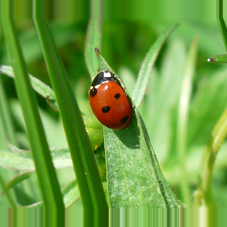
\includegraphics[height=2cm]{data/ladybug.png}
			};

			\newcommand{\outerarrow}{{Latex[length=0.2cm, width=0.3cm]}}
			\draw[-\outerarrow, line width=4pt, draw=gray] (input) to (n00);

		\end{tikzpicture}
	\end{frame}

	% XAI: Prediction
	\begin{frame}{Forklarbar AI: Layerwise relevance propagation}
		\begin{tikzpicture}
			\newcommand{\nodesize}{8pt}
			\newcommand{\hsep}{24pt}
			\newcommand{\vsep}{12pt}

			\newcommand{\arrowwidth}{0.05cm}
			\newcommand{\innerarrow}{{Latex[length=0.1cm, width=0.15cm]}}

			\newcommand{\modellocation}[1]{($ (0, 0) + ####1 $)}

			\node[circle, inner sep=0pt, fill=none, outer sep=0pt, line width=0pt, draw=none] (n00) at \modellocation{(-3 * \hsep, 0)} {};
			\node[] at (-5.5, 1.5) {};
			\node[] at (5.1, -1.2) {};

			\draw[black, fill=gray!20] (n00.center) --
							($ (n00) + (0, 2*\vsep+0.5*\nodesize+2pt) $) --
							($ (n00) + (6*\hsep+0.5*\nodesize+2pt, 2*\vsep+0.5*\nodesize+2pt) $) --
							($ (n00) + (6*\hsep+0.5*\nodesize+2pt, -2*\vsep-0.5*\nodesize-2pt) $) --
							($ (n00) + (0, -2*\vsep-0.5*\nodesize-2pt) $) --
							(n00.center);


			\node[circle, draw=black, minimum size=\nodesize, inner sep=0pt, fill=train-fill!35, outer sep=0pt, line width=0pt, draw=train-fill!35] (n10) at \modellocation{(-2 * \hsep, 2 * \vsep)} {};
			\node[circle, minimum size=\nodesize, inner sep=0pt, fill=train-fill, outer sep=0pt, line width=0pt, draw=train-fill] (n11) at \modellocation{(-2 * \hsep, 1 * \vsep)} {};
			\node[circle, minimum size=\nodesize, inner sep=0pt, fill=train-fill!15, outer sep=0pt, line width=0pt, draw=train-fill!15] (n12) at \modellocation{(-2 * \hsep, 0)} {};
			\node[circle, minimum size=\nodesize, inner sep=0pt, fill=train-fill!85, outer sep=0pt, line width=0pt, draw=train-fill!85] (n13) at \modellocation{(-2 * \hsep, -1 * \vsep)} {};
			\node[circle, minimum size=\nodesize, inner sep=0pt, fill=train-fill!90, outer sep=0pt, line width=0pt, draw=train-fill!90] (n14) at \modellocation{(-2 * \hsep, -2 * \vsep)} {};

			\node[circle, minimum size=\nodesize, inner sep=0pt, fill=train-fill!55, outer sep=0pt, line width=0pt, draw=train-fill!55] (n20) at \modellocation{(-1 * \hsep, 1.5 * \vsep)} {};
			\node[circle, minimum size=\nodesize, inner sep=0pt, fill=train-fill!20, outer sep=0pt, line width=0pt, draw=train-fill!20] (n21) at \modellocation{(-1 * \hsep, 0.5 * \vsep)} {};
			\node[circle, minimum size=\nodesize, inner sep=0pt, fill=train-fill!90, outer sep=0pt, line width=0pt, draw=train-fill!50] (n22) at \modellocation{(-1 * \hsep, -0.5 * \vsep)} {};
			\node[circle, minimum size=\nodesize, inner sep=0pt, fill=train-fill!35, outer sep=0pt, line width=0pt, draw=train-fill!35] (n23) at \modellocation{(-1 * \hsep, -1.5 * \vsep)} {};

			\node[circle, minimum size=\nodesize, inner sep=0pt, fill=train-fill!95, outer sep=0pt, line width=0pt, draw=train-fill!65] (n30) at \modellocation{(0 * \hsep, 1.5 * \vsep)} {};
			\node[circle, minimum size=\nodesize, inner sep=0pt, fill=train-fill!20, outer sep=0pt, line width=0pt, draw=train-fill!20] (n31) at \modellocation{(0 * \hsep, 0.5 * \vsep)} {};
			\node[circle, minimum size=\nodesize, inner sep=0pt, fill=train-fill!90, outer sep=0pt, line width=0pt, draw=train-fill!90] (n32) at \modellocation{(0 * \hsep, -0.5 * \vsep)} {};
			\node[circle, minimum size=\nodesize, inner sep=0pt, fill=train-fill!80, outer sep=0pt, line width=0pt, draw=train-fill!80] (n33) at \modellocation{(0 * \hsep, -1.5 * \vsep)} {};

			\node[circle, minimum size=\nodesize, inner sep=0pt, fill=train-fill!50, outer sep=0pt, line width=0pt, draw=train-fill!50] (n40) at \modellocation{(1 * \hsep, 1*\vsep)} {};
			\node[circle, minimum size=\nodesize, inner sep=0pt, fill=train-fill!90, outer sep=0pt, line width=0pt, draw=train-fill!70] (n41) at \modellocation{(1 * \hsep, 0*\vsep)} {};
			\node[circle, minimum size=\nodesize, inner sep=0pt, fill=train-fill!70, outer sep=0pt, line width=0pt, draw=train-fill!30] (n42) at \modellocation{(1 * \hsep, -1*\vsep)} {};

			\node[circle, minimum size=\nodesize, inner sep=0pt, fill=train-fill, outer sep=0pt, line width=0pt, draw=train-fill] (n50) at \modellocation{(2 * \hsep, 1*\vsep)} {};
			\node[circle, minimum size=\nodesize, inner sep=0pt, fill=train-fill!70, outer sep=0pt, line width=0pt, draw=train-fill!70] (n51) at \modellocation{(2 * \hsep, 0*\vsep)} {};
			\node[circle, minimum size=\nodesize, inner sep=0pt, fill=train-fill!30, outer sep=0pt, line width=0pt, draw=train-fill!30] (n52) at \modellocation{(2 * \hsep, -1*\vsep)} {};

			\node[circle, minimum size=\nodesize, inner sep=0pt, fill=train-fill!80, outer sep=0pt, line width=0pt, draw=train-fill!65] (n60) at \modellocation{(3 * \hsep, 0)} {};

			\draw[
				color=train-fill!35,
				-\innerarrow,
				line width=\arrowwidth
			] (n00) to [out=20,in=200] (n10) {};
			\draw[
				color=train-fill,
				-\innerarrow,
				line width=\arrowwidth
			] (n00) to [out=10,in=190] (n11) {};
			\draw[
				color=train-fill!15,
				-\innerarrow,
				line width=\arrowwidth
			] (n00) to [out=0,in=180] (n12) {};
			\draw[
				color=train-fill!85,
				-\innerarrow,
				line width=\arrowwidth
			] (n00) to [out=-10,in=170] (n13) {};
			\draw[
				color=train-fill!90,
				-\innerarrow,
				line width=\arrowwidth
			] (n00) to [out=-20,in=160] (n14) {};

			\draw[
				color=train-fill!35,
				-\innerarrow,
				line width=\arrowwidth
			] (n10) to [out=-5,in=175] (n20) {};
			\draw[
				color=train-fill!10,
				-\innerarrow,
				line width=\arrowwidth
			] (n10) to [out=-15,in=165] (n21) {};
			\draw[
				color=train-fill!70,
				-\innerarrow,
				line width=\arrowwidth
			] (n10) to [out=-25,in=155] (n22) {};
			\draw[
				color=train-fill!50,
				-\innerarrow,
				line width=\arrowwidth
			] (n10) to [out=-35,in=145] (n23) {};

			\draw[
				color=train-fill!30,
				-\innerarrow,
				line width=\arrowwidth
			] (n11) to [out=5,in=185] (n20) {};
			\draw[
				color=train-fill!25,
				-\innerarrow,
				line width=\arrowwidth
			] (n11) to [out=-5,in=175] (n21) {};
			\draw[
				color=train-fill!95,
				-\innerarrow,
				line width=\arrowwidth
			] (n11) to [out=-15,in=165] (n22) {};
			\draw[
				color=train-fill!35,
				-\innerarrow,
				line width=\arrowwidth
			] (n11) to [out=-25,in=155] (n23) {};

			\draw[
				color=train-fill!70,
				-\innerarrow,
				line width=\arrowwidth
			] (n12) to [out=15,in=195] (n20) {};
			\draw[
				color=train-fill!20,
				-\innerarrow,
				line width=\arrowwidth
			] (n12) to [out=5,in=185] (n21) {};
			\draw[
				color=train-fill!80,
				-\innerarrow,
				line width=\arrowwidth
			] (n12) to [out=-5,in=175] (n22) {};
			\draw[
				color=train-fill,
				-\innerarrow,
				line width=\arrowwidth
			] (n12) to [out=-15,in=165] (n23) {};

			\draw[
				color=train-fill!40,
				-\innerarrow,
				line width=\arrowwidth
			] (n13) to [out=25,in=205] (n20) {};
			\draw[
				color=train-fill!35,
				-\innerarrow,
				line width=\arrowwidth
			] (n13) to [out=15,in=195] (n21) {};
			\draw[
				color=train-fill!20,
				-\innerarrow,
				line width=\arrowwidth
			] (n13) to [out=5,in=185] (n22) {};
			\draw[
				color=white,
				-\innerarrow,
				line width=\arrowwidth
			] (n13) to [out=-5,in=175] (n23) {};

			\draw[
				color=train-fill!40,
				-\innerarrow,
				line width=\arrowwidth
			] (n14) to [out=35,in=215] (n20) {};
			\draw[
				color=train-fill!85,
				-\innerarrow,
				line width=\arrowwidth
			] (n14) to [out=25,in=205] (n21) {};
			\draw[
				color=train-fill!35,
				-\innerarrow,
				line width=\arrowwidth
			] (n14) to [out=15,in=195] (n22) {};
			\draw[
				color=train-fill,
				-\innerarrow,
				line width=\arrowwidth
			] (n14) to [out=5,in=185] (n23) {};

			\draw[
				color=train-fill!85,
				-\innerarrow,
				line width=\arrowwidth
			] (n20) to [out=0,in=180] (n30) {};
			\draw[
				color=train-fill!50,
				-\innerarrow,
				line width=\arrowwidth
			] (n20) to [out=-10,in=170] (n31) {};
			\draw[
				color=train-fill!75,
				-\innerarrow,
				line width=\arrowwidth
			] (n20) to [out=-20,in=160] (n32) {};
			\draw[
				color=white,
				-\innerarrow,
				line width=\arrowwidth
			] (n20) to [out=-30,in=150] (n33) {};

			\draw[
				color=train-fill,
				-\innerarrow,
				line width=\arrowwidth
			] (n21) to [out=10,in=190] (n30) {};
			\draw[
				color=train-fill!30,
				-\innerarrow,
				line width=\arrowwidth
			] (n21) to [out=0,in=180] (n31) {};
			\draw[
				color=train-fill!25,
				-\innerarrow,
				line width=\arrowwidth
			] (n21) to [out=-10,in=170] (n32) {};
			\draw[
				color=white,
				-\innerarrow,
				line width=\arrowwidth
			] (n21) to [out=-20,in=160] (n33) {};

			\draw[
				color=train-fill!35,
				-\innerarrow,
				line width=\arrowwidth
			] (n22) to [out=20,in=200] (n30) {};
			\draw[
				color=train-fill!95,
				-\innerarrow,
				line width=\arrowwidth
			] (n22) to [out=10,in=190] (n31) {};
			\draw[
				color=train-fill!80,
				-\innerarrow,
				line width=\arrowwidth
			] (n22) to [out=0,in=180] (n32) {};
			\draw[
				color=white,
				-\innerarrow,
				line width=\arrowwidth
			] (n22) to [out=-10,in=170] (n33) {};

			\draw[
				color=train-fill!45,
				-\innerarrow,
				line width=\arrowwidth
			] (n23) to [out=30,in=210] (n30) {};
			\draw[
				color=train-fill!70,
				-\innerarrow,
				line width=\arrowwidth
			] (n23) to [out=20,in=200] (n31) {};
			\draw[
				color=train-fill!10,
				-\innerarrow,
				line width=\arrowwidth
			] (n23) to [out=10,in=190] (n32) {};
			\draw[
				color=train-fill!20,
				-\innerarrow,
				line width=\arrowwidth
			] (n23) to [out=0,in=180] (n33) {};

			\draw[
				color=train-fill!50,
				-\innerarrow,
				line width=\arrowwidth
			] (n30) to [out=-5,in=175] (n40) {};
			\draw[
				color=train-fill!30,
				-\innerarrow,
				line width=\arrowwidth
			] (n30) to [out=-15,in=165] (n41) {};
			\draw[
				color=train-fill,
				-\innerarrow,
				line width=\arrowwidth
			] (n30) to [out=-25,in=155] (n42) {};

			\draw[
				color=train-fill!45,
				-\innerarrow,
				line width=\arrowwidth
			] (n31) to [out=5,in=185] (n40) {};
			\draw[
				color=train-fill!90,
				-\innerarrow,
				line width=\arrowwidth
			] (n31) to [out=-5,in=175] (n41) {};
			\draw[
				color=train-fill!45,
				-\innerarrow,
				line width=\arrowwidth
			] (n31) to [out=-15,in=165] (n42) {};

			\draw[
				color=train-fill!15,
				-\innerarrow,
				line width=\arrowwidth
			] (n32) to [out=15,in=195] (n40) {};
			\draw[
				color=train-fill!70,
				-\innerarrow,
				line width=\arrowwidth
			] (n32) to [out=5,in=185] (n41) {};
			\draw[
				color=train-fill!50,
				-\innerarrow,
				line width=\arrowwidth
			] (n32) to [out=-5,in=175] (n42) {};

			\draw[
				color=train-fill!40,
				-\innerarrow,
				line width=\arrowwidth
			] (n33) to [out=25,in=205] (n40) {};
			\draw[
				color=train-fill!20,
				-\innerarrow,
				line width=\arrowwidth
			] (n33) to [out=15,in=195] (n41) {};
			\draw[
				color=train-fill!90,
				-\innerarrow,
				line width=\arrowwidth
			] (n33) to [out=5,in=185] (n42) {};

			\draw[
				color=train-fill!25,
				-\innerarrow,
				line width=\arrowwidth
			] (n40) to [out=0,in=180] (n50) {};
			\draw[
				color=train-fill!15,
				-\innerarrow,
				line width=\arrowwidth
			] (n40) to [out=-10,in=170] (n51) {};
			\draw[
				color=train-fill,
				-\innerarrow,
				line width=\arrowwidth
			] (n40) to [out=-20,in=160] (n52) {};

			\draw[
				color=train-fill!35,
				-\innerarrow,
				line width=\arrowwidth
			] (n41) to [out=10,in=190] (n50) {};
			\draw[
				color=train-fill!10,
				-\innerarrow,
				line width=\arrowwidth
			] (n41) to [out=0,in=180] (n51) {};
			\draw[
				color=train-fill!90,
				-\innerarrow,
				line width=\arrowwidth
			] (n41) to [out=-10,in=170] (n52) {};

			\draw[
				color=train-fill!50,
				-\innerarrow,
				line width=\arrowwidth
			] (n42) to [out=20,in=200] (n50) {};
			\draw[
				color=train-fill!40,
				-\innerarrow,
				line width=\arrowwidth
			] (n42) to [out=10,in=190] (n51) {};
			\draw[
				color=train-fill!20,
				-\innerarrow,
				line width=\arrowwidth
			] (n42) to [out=0,in=180] (n52) {};

			\draw[
				color=train-fill!80,
				-\innerarrow,
				line width=\arrowwidth,
			] (n50) to [out=-10,in=170] (n60) {};
			\draw[
				color=train-fill!90,
				-\innerarrow,
				line width=\arrowwidth,
			] (n51) to [out=0,in=180] (n60) {};
			\draw[
				color=train-fill!30,
				-\innerarrow,
				line width=\arrowwidth,
			] (n52) to [out=10,in=190] (n60) {};


			\node[] at ($ (n30) + (0, \vsep+0.75*\nodesize) $) {Konvolusjonelt nevralt nettverk};

			\node[inner sep=0pt, outer sep=0pt, draw=black] (input) at ($ (n00) - (2, 0) $) {
				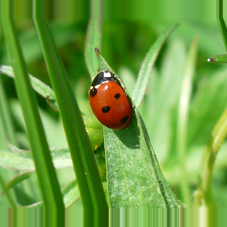
\includegraphics[height=2cm]{data/ladybug.png}
			};
			\node[] (output) at ($ (n60) + (2, 0) $) {
				"marihøne"
			};

			\newcommand{\outerarrow}{{Latex[length=0.2cm, width=0.3cm]}}
			\draw[-\outerarrow, line width=4pt, draw=gray] (input) to (n00);
			\draw[-\outerarrow, line width=4pt, draw=gray] ($ (n60.east) + (0.076, 0) $) to (output);


		\end{tikzpicture}
	\end{frame}

	% XAI: LRP prediction
	\begin{frame}{Forklarbar AI: Layerwise relevance propagation}
		\begin{tikzpicture}
			\newcommand{\nodesize}{8pt}
			\newcommand{\hsep}{24pt}
			\newcommand{\vsep}{12pt}

			\newcommand{\arrowwidth}{0.05cm}
			\newcommand{\innerarrow}{{Latex[length=0.1cm, width=0.15cm]}}

			\newcommand{\modellocation}[1]{($ (0, 0) + ####1 $)}

			\node[circle, inner sep=0pt, fill=none, outer sep=0pt, line width=0pt, draw=none] (n00) at \modellocation{(-3 * \hsep, 0)} {};
			\node[] at (-5.5, 1.5) {};
			\node[] at (5.1, -1.2) {};

			\draw[black, fill=gray!20] (n00.center) --
							($ (n00) + (0, 2*\vsep+0.5*\nodesize+2pt) $) --
							($ (n00) + (6*\hsep+0.5*\nodesize+2pt, 2*\vsep+0.5*\nodesize+2pt) $) --
							($ (n00) + (6*\hsep+0.5*\nodesize+2pt, -2*\vsep-0.5*\nodesize-2pt) $) --
							($ (n00) + (0, -2*\vsep-0.5*\nodesize-2pt) $) --
							(n00.center);


			\node[circle, draw=black, minimum size=\nodesize, inner sep=0pt, fill=train-fill!35, outer sep=0pt, line width=0pt, draw=train-fill!35] (n10) at \modellocation{(-2 * \hsep, 2 * \vsep)} {};
			\node[circle, minimum size=\nodesize, inner sep=0pt, fill=train-fill, outer sep=0pt, line width=0pt, draw=train-fill] (n11) at \modellocation{(-2 * \hsep, 1 * \vsep)} {};
			\node[circle, minimum size=\nodesize, inner sep=0pt, fill=train-fill!15, outer sep=0pt, line width=0pt, draw=train-fill!15] (n12) at \modellocation{(-2 * \hsep, 0)} {};
			\node[circle, minimum size=\nodesize, inner sep=0pt, fill=train-fill!85, outer sep=0pt, line width=0pt, draw=train-fill!85] (n13) at \modellocation{(-2 * \hsep, -1 * \vsep)} {};
			\node[circle, minimum size=\nodesize, inner sep=0pt, fill=train-fill!90, outer sep=0pt, line width=0pt, draw=train-fill!90] (n14) at \modellocation{(-2 * \hsep, -2 * \vsep)} {};

			\node[circle, minimum size=\nodesize, inner sep=0pt, fill=train-fill!55, outer sep=0pt, line width=0pt, draw=train-fill!55] (n20) at \modellocation{(-1 * \hsep, 1.5 * \vsep)} {};
			\node[circle, minimum size=\nodesize, inner sep=0pt, fill=train-fill!20, outer sep=0pt, line width=0pt, draw=train-fill!20] (n21) at \modellocation{(-1 * \hsep, 0.5 * \vsep)} {};
			\node[circle, minimum size=\nodesize, inner sep=0pt, fill=train-fill!90, outer sep=0pt, line width=0pt, draw=train-fill!50] (n22) at \modellocation{(-1 * \hsep, -0.5 * \vsep)} {};
			\node[circle, minimum size=\nodesize, inner sep=0pt, fill=train-fill!35, outer sep=0pt, line width=0pt, draw=train-fill!35] (n23) at \modellocation{(-1 * \hsep, -1.5 * \vsep)} {};

			\node[circle, minimum size=\nodesize, inner sep=0pt, fill=train-fill!95, outer sep=0pt, line width=0pt, draw=train-fill!65] (n30) at \modellocation{(0 * \hsep, 1.5 * \vsep)} {};
			\node[circle, minimum size=\nodesize, inner sep=0pt, fill=train-fill!20, outer sep=0pt, line width=0pt, draw=train-fill!20] (n31) at \modellocation{(0 * \hsep, 0.5 * \vsep)} {};
			\node[circle, minimum size=\nodesize, inner sep=0pt, fill=train-fill!90, outer sep=0pt, line width=0pt, draw=train-fill!90] (n32) at \modellocation{(0 * \hsep, -0.5 * \vsep)} {};
			\node[circle, minimum size=\nodesize, inner sep=0pt, fill=train-fill!80, outer sep=0pt, line width=0pt, draw=train-fill!80] (n33) at \modellocation{(0 * \hsep, -1.5 * \vsep)} {};

			\node[circle, minimum size=\nodesize, inner sep=0pt, fill=train-fill!50, outer sep=0pt, line width=0pt, draw=train-fill!50] (n40) at \modellocation{(1 * \hsep, 1*\vsep)} {};
			\node[circle, minimum size=\nodesize, inner sep=0pt, fill=train-fill!90, outer sep=0pt, line width=0pt, draw=train-fill!70] (n41) at \modellocation{(1 * \hsep, 0*\vsep)} {};
			\node[circle, minimum size=\nodesize, inner sep=0pt, fill=train-fill!70, outer sep=0pt, line width=0pt, draw=train-fill!30] (n42) at \modellocation{(1 * \hsep, -1*\vsep)} {};

			\node[circle, minimum size=\nodesize, inner sep=0pt, fill=train-fill, outer sep=0pt, line width=0pt, draw=train-fill] (n50) at \modellocation{(2 * \hsep, 1*\vsep)} {};
			\node[circle, minimum size=\nodesize, inner sep=0pt, fill=train-fill!70, outer sep=0pt, line width=0pt, draw=train-fill!70] (n51) at \modellocation{(2 * \hsep, 0*\vsep)} {};
			\node[circle, minimum size=\nodesize, inner sep=0pt, fill=train-fill!30, outer sep=0pt, line width=0pt, draw=train-fill!30] (n52) at \modellocation{(2 * \hsep, -1*\vsep)} {};

			\node[circle, minimum size=\nodesize, inner sep=0pt, fill={rgb:orange,7;yellow,4;black,1}, outer sep=0pt, line width=0pt, draw={rgb:orange,7;yellow,4;black,1}] (n60) at \modellocation{(3 * \hsep, 0)} {};

			\draw[
				color=train-fill!35,
				-\innerarrow,
				line width=\arrowwidth
			] (n00) to [out=20,in=200] (n10) {};
			\draw[
				color=train-fill,
				-\innerarrow,
				line width=\arrowwidth
			] (n00) to [out=10,in=190] (n11) {};
			\draw[
				color=train-fill!15,
				-\innerarrow,
				line width=\arrowwidth
			] (n00) to [out=0,in=180] (n12) {};
			\draw[
				color=train-fill!85,
				-\innerarrow,
				line width=\arrowwidth
			] (n00) to [out=-10,in=170] (n13) {};
			\draw[
				color=train-fill!90,
				-\innerarrow,
				line width=\arrowwidth
			] (n00) to [out=-20,in=160] (n14) {};

			\draw[
				color=train-fill!35,
				-\innerarrow,
				line width=\arrowwidth
			] (n10) to [out=-5,in=175] (n20) {};
			\draw[
				color=train-fill!10,
				-\innerarrow,
				line width=\arrowwidth
			] (n10) to [out=-15,in=165] (n21) {};
			\draw[
				color=train-fill!70,
				-\innerarrow,
				line width=\arrowwidth
			] (n10) to [out=-25,in=155] (n22) {};
			\draw[
				color=train-fill!50,
				-\innerarrow,
				line width=\arrowwidth
			] (n10) to [out=-35,in=145] (n23) {};

			\draw[
				color=train-fill!30,
				-\innerarrow,
				line width=\arrowwidth
			] (n11) to [out=5,in=185] (n20) {};
			\draw[
				color=train-fill!25,
				-\innerarrow,
				line width=\arrowwidth
			] (n11) to [out=-5,in=175] (n21) {};
			\draw[
				color=train-fill!95,
				-\innerarrow,
				line width=\arrowwidth
			] (n11) to [out=-15,in=165] (n22) {};
			\draw[
				color=train-fill!35,
				-\innerarrow,
				line width=\arrowwidth
			] (n11) to [out=-25,in=155] (n23) {};

			\draw[
				color=train-fill!70,
				-\innerarrow,
				line width=\arrowwidth
			] (n12) to [out=15,in=195] (n20) {};
			\draw[
				color=train-fill!20,
				-\innerarrow,
				line width=\arrowwidth
			] (n12) to [out=5,in=185] (n21) {};
			\draw[
				color=train-fill!80,
				-\innerarrow,
				line width=\arrowwidth
			] (n12) to [out=-5,in=175] (n22) {};
			\draw[
				color=train-fill,
				-\innerarrow,
				line width=\arrowwidth
			] (n12) to [out=-15,in=165] (n23) {};

			\draw[
				color=train-fill!40,
				-\innerarrow,
				line width=\arrowwidth
			] (n13) to [out=25,in=205] (n20) {};
			\draw[
				color=train-fill!35,
				-\innerarrow,
				line width=\arrowwidth
			] (n13) to [out=15,in=195] (n21) {};
			\draw[
				color=train-fill!20,
				-\innerarrow,
				line width=\arrowwidth
			] (n13) to [out=5,in=185] (n22) {};
			\draw[
				color=white,
				-\innerarrow,
				line width=\arrowwidth
			] (n13) to [out=-5,in=175] (n23) {};

			\draw[
				color=train-fill!40,
				-\innerarrow,
				line width=\arrowwidth
			] (n14) to [out=35,in=215] (n20) {};
			\draw[
				color=train-fill!85,
				-\innerarrow,
				line width=\arrowwidth
			] (n14) to [out=25,in=205] (n21) {};
			\draw[
				color=train-fill!35,
				-\innerarrow,
				line width=\arrowwidth
			] (n14) to [out=15,in=195] (n22) {};
			\draw[
				color=train-fill,
				-\innerarrow,
				line width=\arrowwidth
			] (n14) to [out=5,in=185] (n23) {};

			\draw[
				color=train-fill!85,
				-\innerarrow,
				line width=\arrowwidth
			] (n20) to [out=0,in=180] (n30) {};
			\draw[
				color=train-fill!50,
				-\innerarrow,
				line width=\arrowwidth
			] (n20) to [out=-10,in=170] (n31) {};
			\draw[
				color=train-fill!75,
				-\innerarrow,
				line width=\arrowwidth
			] (n20) to [out=-20,in=160] (n32) {};
			\draw[
				color=white,
				-\innerarrow,
				line width=\arrowwidth
			] (n20) to [out=-30,in=150] (n33) {};

			\draw[
				color=train-fill,
				-\innerarrow,
				line width=\arrowwidth
			] (n21) to [out=10,in=190] (n30) {};
			\draw[
				color=train-fill!30,
				-\innerarrow,
				line width=\arrowwidth
			] (n21) to [out=0,in=180] (n31) {};
			\draw[
				color=train-fill!25,
				-\innerarrow,
				line width=\arrowwidth
			] (n21) to [out=-10,in=170] (n32) {};
			\draw[
				color=white,
				-\innerarrow,
				line width=\arrowwidth
			] (n21) to [out=-20,in=160] (n33) {};

			\draw[
				color=train-fill!35,
				-\innerarrow,
				line width=\arrowwidth
			] (n22) to [out=20,in=200] (n30) {};
			\draw[
				color=train-fill!95,
				-\innerarrow,
				line width=\arrowwidth
			] (n22) to [out=10,in=190] (n31) {};
			\draw[
				color=train-fill!80,
				-\innerarrow,
				line width=\arrowwidth
			] (n22) to [out=0,in=180] (n32) {};
			\draw[
				color=white,
				-\innerarrow,
				line width=\arrowwidth
			] (n22) to [out=-10,in=170] (n33) {};

			\draw[
				color=train-fill!45,
				-\innerarrow,
				line width=\arrowwidth
			] (n23) to [out=30,in=210] (n30) {};
			\draw[
				color=train-fill!70,
				-\innerarrow,
				line width=\arrowwidth
			] (n23) to [out=20,in=200] (n31) {};
			\draw[
				color=train-fill!10,
				-\innerarrow,
				line width=\arrowwidth
			] (n23) to [out=10,in=190] (n32) {};
			\draw[
				color=train-fill!20,
				-\innerarrow,
				line width=\arrowwidth
			] (n23) to [out=0,in=180] (n33) {};

			\draw[
				color=train-fill!50,
				-\innerarrow,
				line width=\arrowwidth
			] (n30) to [out=-5,in=175] (n40) {};
			\draw[
				color=train-fill!30,
				-\innerarrow,
				line width=\arrowwidth
			] (n30) to [out=-15,in=165] (n41) {};
			\draw[
				color=train-fill,
				-\innerarrow,
				line width=\arrowwidth
			] (n30) to [out=-25,in=155] (n42) {};

			\draw[
				color=train-fill!45,
				-\innerarrow,
				line width=\arrowwidth
			] (n31) to [out=5,in=185] (n40) {};
			\draw[
				color=train-fill!90,
				-\innerarrow,
				line width=\arrowwidth
			] (n31) to [out=-5,in=175] (n41) {};
			\draw[
				color=train-fill!45,
				-\innerarrow,
				line width=\arrowwidth
			] (n31) to [out=-15,in=165] (n42) {};

			\draw[
				color=train-fill!15,
				-\innerarrow,
				line width=\arrowwidth
			] (n32) to [out=15,in=195] (n40) {};
			\draw[
				color=train-fill!70,
				-\innerarrow,
				line width=\arrowwidth
			] (n32) to [out=5,in=185] (n41) {};
			\draw[
				color=train-fill!50,
				-\innerarrow,
				line width=\arrowwidth
			] (n32) to [out=-5,in=175] (n42) {};

			\draw[
				color=train-fill!40,
				-\innerarrow,
				line width=\arrowwidth
			] (n33) to [out=25,in=205] (n40) {};
			\draw[
				color=train-fill!20,
				-\innerarrow,
				line width=\arrowwidth
			] (n33) to [out=15,in=195] (n41) {};
			\draw[
				color=train-fill!90,
				-\innerarrow,
				line width=\arrowwidth
			] (n33) to [out=5,in=185] (n42) {};

			\draw[
				color=train-fill!25,
				-\innerarrow,
				line width=\arrowwidth
			] (n40) to [out=0,in=180] (n50) {};
			\draw[
				color=train-fill!15,
				-\innerarrow,
				line width=\arrowwidth
			] (n40) to [out=-10,in=170] (n51) {};
			\draw[
				color=train-fill,
				-\innerarrow,
				line width=\arrowwidth
			] (n40) to [out=-20,in=160] (n52) {};

			\draw[
				color=train-fill!35,
				-\innerarrow,
				line width=\arrowwidth
			] (n41) to [out=10,in=190] (n50) {};
			\draw[
				color=train-fill!10,
				-\innerarrow,
				line width=\arrowwidth
			] (n41) to [out=0,in=180] (n51) {};
			\draw[
				color=train-fill!90,
				-\innerarrow,
				line width=\arrowwidth
			] (n41) to [out=-10,in=170] (n52) {};

			\draw[
				color=train-fill!50,
				-\innerarrow,
				line width=\arrowwidth
			] (n42) to [out=20,in=200] (n50) {};
			\draw[
				color=train-fill!40,
				-\innerarrow,
				line width=\arrowwidth
			] (n42) to [out=10,in=190] (n51) {};
			\draw[
				color=train-fill!20,
				-\innerarrow,
				line width=\arrowwidth
			] (n42) to [out=0,in=180] (n52) {};

			\draw[
				color=train-fill!80,
				-\innerarrow,
				line width=\arrowwidth,
			] (n50) to [out=-10,in=170] (n60) {};
			\draw[
				color=train-fill!90,
				-\innerarrow,
				line width=\arrowwidth,
			] (n51) to [out=0,in=180] (n60) {};
			\draw[
				color=train-fill!30,
				-\innerarrow,
				line width=\arrowwidth,
			] (n52) to [out=10,in=190] (n60) {};


			\node[] at ($ (n30) + (0, \vsep+0.75*\nodesize) $) {Konvolusjonelt nevralt nettverk};

			\node[inner sep=0pt, outer sep=0pt, draw=black] (input) at ($ (n00) - (2, 0) $) {
				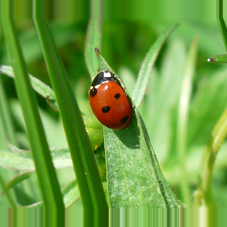
\includegraphics[height=2cm]{data/ladybug.png}
			};
			\node[] (output) at ($ (n60) + (2, 0) $) {
				"marihøne"
			};

			\newcommand{\outerarrow}{{Latex[length=0.2cm, width=0.3cm]}}
			\draw[-\outerarrow, line width=4pt, draw=gray] (input) to (n00);
			\draw[-\outerarrow, line width=4pt, draw=gray] (output) to ($ (n60.east) + (0.076, 0) $);


		\end{tikzpicture}
	\end{frame}

	% XAI: LRP first layer
	\begin{frame}{Forklarbar AI: Layerwise relevance propagation}
		\begin{tikzpicture}
			\newcommand{\nodesize}{8pt}
			\newcommand{\hsep}{24pt}
			\newcommand{\vsep}{12pt}

			\newcommand{\arrowwidth}{0.05cm}
			\newcommand{\innerarrow}{{Latex[length=0.1cm, width=0.15cm]}}

			\newcommand{\modellocation}[1]{($ (0, 0) + ####1 $)}

			\node[circle, inner sep=0pt, fill=none, outer sep=0pt, line width=0pt, draw=none] (n00) at \modellocation{(-3 * \hsep, 0)} {};
			\node[] at (-5.5, 1.5) {};
			\node[] at (5.1, -1.2) {};

			\draw[black, fill=gray!20] (n00.center) --
							($ (n00) + (0, 2*\vsep+0.5*\nodesize+2pt) $) --
							($ (n00) + (6*\hsep+0.5*\nodesize+2pt, 2*\vsep+0.5*\nodesize+2pt) $) --
							($ (n00) + (6*\hsep+0.5*\nodesize+2pt, -2*\vsep-0.5*\nodesize-2pt) $) --
							($ (n00) + (0, -2*\vsep-0.5*\nodesize-2pt) $) --
							(n00.center);


			\node[circle, draw=black, minimum size=\nodesize, inner sep=0pt, fill=train-fill!35, outer sep=0pt, line width=0pt, draw=train-fill!35] (n10) at \modellocation{(-2 * \hsep, 2 * \vsep)} {};
			\node[circle, minimum size=\nodesize, inner sep=0pt, fill=train-fill, outer sep=0pt, line width=0pt, draw=train-fill] (n11) at \modellocation{(-2 * \hsep, 1 * \vsep)} {};
			\node[circle, minimum size=\nodesize, inner sep=0pt, fill=train-fill!15, outer sep=0pt, line width=0pt, draw=train-fill!15] (n12) at \modellocation{(-2 * \hsep, 0)} {};
			\node[circle, minimum size=\nodesize, inner sep=0pt, fill=train-fill!85, outer sep=0pt, line width=0pt, draw=train-fill!85] (n13) at \modellocation{(-2 * \hsep, -1 * \vsep)} {};
			\node[circle, minimum size=\nodesize, inner sep=0pt, fill=train-fill!90, outer sep=0pt, line width=0pt, draw=train-fill!90] (n14) at \modellocation{(-2 * \hsep, -2 * \vsep)} {};

			\node[circle, minimum size=\nodesize, inner sep=0pt, fill=train-fill!55, outer sep=0pt, line width=0pt, draw=train-fill!55] (n20) at \modellocation{(-1 * \hsep, 1.5 * \vsep)} {};
			\node[circle, minimum size=\nodesize, inner sep=0pt, fill=train-fill!20, outer sep=0pt, line width=0pt, draw=train-fill!20] (n21) at \modellocation{(-1 * \hsep, 0.5 * \vsep)} {};
			\node[circle, minimum size=\nodesize, inner sep=0pt, fill=train-fill!90, outer sep=0pt, line width=0pt, draw=train-fill!50] (n22) at \modellocation{(-1 * \hsep, -0.5 * \vsep)} {};
			\node[circle, minimum size=\nodesize, inner sep=0pt, fill=train-fill!35, outer sep=0pt, line width=0pt, draw=train-fill!35] (n23) at \modellocation{(-1 * \hsep, -1.5 * \vsep)} {};

			\node[circle, minimum size=\nodesize, inner sep=0pt, fill=train-fill!95, outer sep=0pt, line width=0pt, draw=train-fill!65] (n30) at \modellocation{(0 * \hsep, 1.5 * \vsep)} {};
			\node[circle, minimum size=\nodesize, inner sep=0pt, fill=train-fill!20, outer sep=0pt, line width=0pt, draw=train-fill!20] (n31) at \modellocation{(0 * \hsep, 0.5 * \vsep)} {};
			\node[circle, minimum size=\nodesize, inner sep=0pt, fill=train-fill!90, outer sep=0pt, line width=0pt, draw=train-fill!90] (n32) at \modellocation{(0 * \hsep, -0.5 * \vsep)} {};
			\node[circle, minimum size=\nodesize, inner sep=0pt, fill=train-fill!80, outer sep=0pt, line width=0pt, draw=train-fill!80] (n33) at \modellocation{(0 * \hsep, -1.5 * \vsep)} {};

			\node[circle, minimum size=\nodesize, inner sep=0pt, fill=train-fill!50, outer sep=0pt, line width=0pt, draw=train-fill!50] (n40) at \modellocation{(1 * \hsep, 1*\vsep)} {};
			\node[circle, minimum size=\nodesize, inner sep=0pt, fill=train-fill!90, outer sep=0pt, line width=0pt, draw=train-fill!70] (n41) at \modellocation{(1 * \hsep, 0*\vsep)} {};
			\node[circle, minimum size=\nodesize, inner sep=0pt, fill=train-fill!70, outer sep=0pt, line width=0pt, draw=train-fill!30] (n42) at \modellocation{(1 * \hsep, -1*\vsep)} {};

			\node[circle, minimum size=\nodesize, inner sep=0pt, fill={rgb:red,5;black,1;yellow,2}, outer sep=0pt, line width=0pt, draw={rgb:red,5;black,1;yellow,2}] (n50) at \modellocation{(2 * \hsep, 1*\vsep)} {};
			\node[circle, minimum size=\nodesize, inner sep=0pt, fill={rgb:gray,5;red,1}, outer sep=0pt, line width=0pt, draw={rgb:gray,5;red,1}] (n51) at \modellocation{(2 * \hsep, 0*\vsep)} {};
			\node[circle, minimum size=\nodesize, inner sep=0pt, fill={rgb:yellow,5;orange,1}, outer sep=0pt, line width=0pt, draw={rgb:yellow,5;orange,1}] (n52) at \modellocation{(2 * \hsep, -1*\vsep)} {};

			\node[circle, minimum size=\nodesize, inner sep=0pt, fill={rgb:orange,7;yellow,4;black,1}, outer sep=0pt, line width=0pt, draw={rgb:orange,7;yellow,4;black,1}] (n60) at \modellocation{(3 * \hsep, 0)} {};

			\draw[
				color=train-fill!35,
				-\innerarrow,
				line width=\arrowwidth
			] (n00) to [out=20,in=200] (n10) {};
			\draw[
				color=train-fill,
				-\innerarrow,
				line width=\arrowwidth
			] (n00) to [out=10,in=190] (n11) {};
			\draw[
				color=train-fill!15,
				-\innerarrow,
				line width=\arrowwidth
			] (n00) to [out=0,in=180] (n12) {};
			\draw[
				color=train-fill!85,
				-\innerarrow,
				line width=\arrowwidth
			] (n00) to [out=-10,in=170] (n13) {};
			\draw[
				color=train-fill!90,
				-\innerarrow,
				line width=\arrowwidth
			] (n00) to [out=-20,in=160] (n14) {};

			\draw[
				color=train-fill!35,
				-\innerarrow,
				line width=\arrowwidth
			] (n10) to [out=-5,in=175] (n20) {};
			\draw[
				color=train-fill!10,
				-\innerarrow,
				line width=\arrowwidth
			] (n10) to [out=-15,in=165] (n21) {};
			\draw[
				color=train-fill!70,
				-\innerarrow,
				line width=\arrowwidth
			] (n10) to [out=-25,in=155] (n22) {};
			\draw[
				color=train-fill!50,
				-\innerarrow,
				line width=\arrowwidth
			] (n10) to [out=-35,in=145] (n23) {};

			\draw[
				color=train-fill!30,
				-\innerarrow,
				line width=\arrowwidth
			] (n11) to [out=5,in=185] (n20) {};
			\draw[
				color=train-fill!25,
				-\innerarrow,
				line width=\arrowwidth
			] (n11) to [out=-5,in=175] (n21) {};
			\draw[
				color=train-fill!95,
				-\innerarrow,
				line width=\arrowwidth
			] (n11) to [out=-15,in=165] (n22) {};
			\draw[
				color=train-fill!35,
				-\innerarrow,
				line width=\arrowwidth
			] (n11) to [out=-25,in=155] (n23) {};

			\draw[
				color=train-fill!70,
				-\innerarrow,
				line width=\arrowwidth
			] (n12) to [out=15,in=195] (n20) {};
			\draw[
				color=train-fill!20,
				-\innerarrow,
				line width=\arrowwidth
			] (n12) to [out=5,in=185] (n21) {};
			\draw[
				color=train-fill!80,
				-\innerarrow,
				line width=\arrowwidth
			] (n12) to [out=-5,in=175] (n22) {};
			\draw[
				color=train-fill,
				-\innerarrow,
				line width=\arrowwidth
			] (n12) to [out=-15,in=165] (n23) {};

			\draw[
				color=train-fill!40,
				-\innerarrow,
				line width=\arrowwidth
			] (n13) to [out=25,in=205] (n20) {};
			\draw[
				color=train-fill!35,
				-\innerarrow,
				line width=\arrowwidth
			] (n13) to [out=15,in=195] (n21) {};
			\draw[
				color=train-fill!20,
				-\innerarrow,
				line width=\arrowwidth
			] (n13) to [out=5,in=185] (n22) {};
			\draw[
				color=white,
				-\innerarrow,
				line width=\arrowwidth
			] (n13) to [out=-5,in=175] (n23) {};

			\draw[
				color=train-fill!40,
				-\innerarrow,
				line width=\arrowwidth
			] (n14) to [out=35,in=215] (n20) {};
			\draw[
				color=train-fill!85,
				-\innerarrow,
				line width=\arrowwidth
			] (n14) to [out=25,in=205] (n21) {};
			\draw[
				color=train-fill!35,
				-\innerarrow,
				line width=\arrowwidth
			] (n14) to [out=15,in=195] (n22) {};
			\draw[
				color=train-fill,
				-\innerarrow,
				line width=\arrowwidth
			] (n14) to [out=5,in=185] (n23) {};

			\draw[
				color=train-fill!85,
				-\innerarrow,
				line width=\arrowwidth
			] (n20) to [out=0,in=180] (n30) {};
			\draw[
				color=train-fill!50,
				-\innerarrow,
				line width=\arrowwidth
			] (n20) to [out=-10,in=170] (n31) {};
			\draw[
				color=train-fill!75,
				-\innerarrow,
				line width=\arrowwidth
			] (n20) to [out=-20,in=160] (n32) {};
			\draw[
				color=white,
				-\innerarrow,
				line width=\arrowwidth
			] (n20) to [out=-30,in=150] (n33) {};

			\draw[
				color=train-fill,
				-\innerarrow,
				line width=\arrowwidth
			] (n21) to [out=10,in=190] (n30) {};
			\draw[
				color=train-fill!30,
				-\innerarrow,
				line width=\arrowwidth
			] (n21) to [out=0,in=180] (n31) {};
			\draw[
				color=train-fill!25,
				-\innerarrow,
				line width=\arrowwidth
			] (n21) to [out=-10,in=170] (n32) {};
			\draw[
				color=white,
				-\innerarrow,
				line width=\arrowwidth
			] (n21) to [out=-20,in=160] (n33) {};

			\draw[
				color=train-fill!35,
				-\innerarrow,
				line width=\arrowwidth
			] (n22) to [out=20,in=200] (n30) {};
			\draw[
				color=train-fill!95,
				-\innerarrow,
				line width=\arrowwidth
			] (n22) to [out=10,in=190] (n31) {};
			\draw[
				color=train-fill!80,
				-\innerarrow,
				line width=\arrowwidth
			] (n22) to [out=0,in=180] (n32) {};
			\draw[
				color=white,
				-\innerarrow,
				line width=\arrowwidth
			] (n22) to [out=-10,in=170] (n33) {};

			\draw[
				color=train-fill!45,
				-\innerarrow,
				line width=\arrowwidth
			] (n23) to [out=30,in=210] (n30) {};
			\draw[
				color=train-fill!70,
				-\innerarrow,
				line width=\arrowwidth
			] (n23) to [out=20,in=200] (n31) {};
			\draw[
				color=train-fill!10,
				-\innerarrow,
				line width=\arrowwidth
			] (n23) to [out=10,in=190] (n32) {};
			\draw[
				color=train-fill!20,
				-\innerarrow,
				line width=\arrowwidth
			] (n23) to [out=0,in=180] (n33) {};

			\draw[
				color=train-fill!50,
				-\innerarrow,
				line width=\arrowwidth
			] (n30) to [out=-5,in=175] (n40) {};
			\draw[
				color=train-fill!30,
				-\innerarrow,
				line width=\arrowwidth
			] (n30) to [out=-15,in=165] (n41) {};
			\draw[
				color=train-fill,
				-\innerarrow,
				line width=\arrowwidth
			] (n30) to [out=-25,in=155] (n42) {};

			\draw[
				color=train-fill!45,
				-\innerarrow,
				line width=\arrowwidth
			] (n31) to [out=5,in=185] (n40) {};
			\draw[
				color=train-fill!90,
				-\innerarrow,
				line width=\arrowwidth
			] (n31) to [out=-5,in=175] (n41) {};
			\draw[
				color=train-fill!45,
				-\innerarrow,
				line width=\arrowwidth
			] (n31) to [out=-15,in=165] (n42) {};

			\draw[
				color=train-fill!15,
				-\innerarrow,
				line width=\arrowwidth
			] (n32) to [out=15,in=195] (n40) {};
			\draw[
				color=train-fill!70,
				-\innerarrow,
				line width=\arrowwidth
			] (n32) to [out=5,in=185] (n41) {};
			\draw[
				color=train-fill!50,
				-\innerarrow,
				line width=\arrowwidth
			] (n32) to [out=-5,in=175] (n42) {};

			\draw[
				color=train-fill!40,
				-\innerarrow,
				line width=\arrowwidth
			] (n33) to [out=25,in=205] (n40) {};
			\draw[
				color=train-fill!20,
				-\innerarrow,
				line width=\arrowwidth
			] (n33) to [out=15,in=195] (n41) {};
			\draw[
				color=train-fill!90,
				-\innerarrow,
				line width=\arrowwidth
			] (n33) to [out=5,in=185] (n42) {};

			\draw[
				color=train-fill!25,
				-\innerarrow,
				line width=\arrowwidth
			] (n40) to [out=0,in=180] (n50) {};
			\draw[
				color=train-fill!15,
				-\innerarrow,
				line width=\arrowwidth
			] (n40) to [out=-10,in=170] (n51) {};
			\draw[
				color=train-fill,
				-\innerarrow,
				line width=\arrowwidth
			] (n40) to [out=-20,in=160] (n52) {};

			\draw[
				color=train-fill!35,
				-\innerarrow,
				line width=\arrowwidth
			] (n41) to [out=10,in=190] (n50) {};
			\draw[
				color=train-fill!10,
				-\innerarrow,
				line width=\arrowwidth
			] (n41) to [out=0,in=180] (n51) {};
			\draw[
				color=train-fill!90,
				-\innerarrow,
				line width=\arrowwidth
			] (n41) to [out=-10,in=170] (n52) {};

			\draw[
				color=train-fill!50,
				-\innerarrow,
				line width=\arrowwidth
			] (n42) to [out=20,in=200] (n50) {};
			\draw[
				color=train-fill!40,
				-\innerarrow,
				line width=\arrowwidth
			] (n42) to [out=10,in=190] (n51) {};
			\draw[
				color=train-fill!20,
				-\innerarrow,
				line width=\arrowwidth
			] (n42) to [out=0,in=180] (n52) {};

			\draw[
				color={rgb:red,5;black,1;yellow,2},
				\innerarrow-,
				line width=\arrowwidth
			] (n50) to [out=-10,in=170] (n60) {};
			\draw[
				color={rgb:gray,5;red,1},
				\innerarrow-,
				line width=\arrowwidth
			] (n51) to [out=0,in=180] (n60) {};
			\draw[
				color={rgb:yellow,5;orange,1},
				\innerarrow-,
				line width=\arrowwidth
			] (n52) to [out=10,in=190] (n60) {};


			\node[] at ($ (n30) + (0, \vsep+0.75*\nodesize) $) {Konvolusjonelt nevralt nettverk};

			\node[inner sep=0pt, outer sep=0pt, draw=black] (input) at ($ (n00) - (2, 0) $) {
				\includegraphics[height=2cm]{data/ladybug.png}
			};
			\node[] (output) at ($ (n60) + (2, 0) $) {
				"marihøne"
			};

			\newcommand{\outerarrow}{{Latex[length=0.2cm, width=0.3cm]}}
			\draw[-\outerarrow, line width=4pt, draw=gray] (input) to (n00);
			\draw[-\outerarrow, line width=4pt, draw=gray] (output) to ($ (n60.east) + (0.076, 0) $);


		\end{tikzpicture}
	\end{frame}

	% XAI: LRP second layer
	\begin{frame}{Forklarbar AI: Layerwise relevance propagation}
		\begin{tikzpicture}
			\newcommand{\nodesize}{8pt}
			\newcommand{\hsep}{24pt}
			\newcommand{\vsep}{12pt}

			\newcommand{\arrowwidth}{0.05cm}
			\newcommand{\innerarrow}{{Latex[length=0.1cm, width=0.15cm]}}

			\newcommand{\modellocation}[1]{($ (0, 0) + ####1 $)}

			\node[circle, inner sep=0pt, fill=none, outer sep=0pt, line width=0pt, draw=none] (n00) at \modellocation{(-3 * \hsep, 0)} {};
			\node[] at (-5.5, 1.5) {};
			\node[] at (5.1, -1.2) {};

			\draw[black, fill=gray!20] (n00.center) --
							($ (n00) + (0, 2*\vsep+0.5*\nodesize+2pt) $) --
							($ (n00) + (6*\hsep+0.5*\nodesize+2pt, 2*\vsep+0.5*\nodesize+2pt) $) --
							($ (n00) + (6*\hsep+0.5*\nodesize+2pt, -2*\vsep-0.5*\nodesize-2pt) $) --
							($ (n00) + (0, -2*\vsep-0.5*\nodesize-2pt) $) --
							(n00.center);


			\node[circle, draw=black, minimum size=\nodesize, inner sep=0pt, fill=train-fill!35, outer sep=0pt, line width=0pt, draw=train-fill!35] (n10) at \modellocation{(-2 * \hsep, 2 * \vsep)} {};
			\node[circle, minimum size=\nodesize, inner sep=0pt, fill=train-fill, outer sep=0pt, line width=0pt, draw=train-fill] (n11) at \modellocation{(-2 * \hsep, 1 * \vsep)} {};
			\node[circle, minimum size=\nodesize, inner sep=0pt, fill=train-fill!15, outer sep=0pt, line width=0pt, draw=train-fill!15] (n12) at \modellocation{(-2 * \hsep, 0)} {};
			\node[circle, minimum size=\nodesize, inner sep=0pt, fill=train-fill!85, outer sep=0pt, line width=0pt, draw=train-fill!85] (n13) at \modellocation{(-2 * \hsep, -1 * \vsep)} {};
			\node[circle, minimum size=\nodesize, inner sep=0pt, fill=train-fill!90, outer sep=0pt, line width=0pt, draw=train-fill!90] (n14) at \modellocation{(-2 * \hsep, -2 * \vsep)} {};

			\node[circle, minimum size=\nodesize, inner sep=0pt, fill=train-fill!55, outer sep=0pt, line width=0pt, draw=train-fill!55] (n20) at \modellocation{(-1 * \hsep, 1.5 * \vsep)} {};
			\node[circle, minimum size=\nodesize, inner sep=0pt, fill=train-fill!20, outer sep=0pt, line width=0pt, draw=train-fill!20] (n21) at \modellocation{(-1 * \hsep, 0.5 * \vsep)} {};
			\node[circle, minimum size=\nodesize, inner sep=0pt, fill=train-fill!90, outer sep=0pt, line width=0pt, draw=train-fill!50] (n22) at \modellocation{(-1 * \hsep, -0.5 * \vsep)} {};
			\node[circle, minimum size=\nodesize, inner sep=0pt, fill=train-fill!35, outer sep=0pt, line width=0pt, draw=train-fill!35] (n23) at \modellocation{(-1 * \hsep, -1.5 * \vsep)} {};

			\node[circle, minimum size=\nodesize, inner sep=0pt, fill=train-fill!95, outer sep=0pt, line width=0pt, draw=train-fill!65] (n30) at \modellocation{(0 * \hsep, 1.5 * \vsep)} {};
			\node[circle, minimum size=\nodesize, inner sep=0pt, fill=train-fill!20, outer sep=0pt, line width=0pt, draw=train-fill!20] (n31) at \modellocation{(0 * \hsep, 0.5 * \vsep)} {};
			\node[circle, minimum size=\nodesize, inner sep=0pt, fill=train-fill!90, outer sep=0pt, line width=0pt, draw=train-fill!90] (n32) at \modellocation{(0 * \hsep, -0.5 * \vsep)} {};
			\node[circle, minimum size=\nodesize, inner sep=0pt, fill=train-fill!80, outer sep=0pt, line width=0pt, draw=train-fill!80] (n33) at \modellocation{(0 * \hsep, -1.5 * \vsep)} {};

			\node[circle, minimum size=\nodesize, inner sep=0pt, fill={rgb:yellow,10;orange,1}, outer sep=0pt, line width=0pt, draw={rgb:yellow,10;orange,1}] (n40) at \modellocation{(1 * \hsep, 1*\vsep)} {};
			\node[circle, minimum size=\nodesize, inner sep=0pt, fill={rgb:red,1}, outer sep=0pt, line width=0pt, draw={rgb:red,1}] (n41) at \modellocation{(1 * \hsep, 0*\vsep)} {};
			\node[circle, minimum size=\nodesize, inner sep=0pt, fill={rgb:black,10;white,15;red,2}, outer sep=0pt, line width=0pt, draw={rgb:black,10;white,15;red,2}] (n42) at \modellocation{(1 * \hsep, -1*\vsep)} {};

			\node[circle, minimum size=\nodesize, inner sep=0pt, fill={rgb:red,5;black,1;yellow,2}, outer sep=0pt, line width=0pt, draw={rgb:red,5;black,1;yellow,2}] (n50) at \modellocation{(2 * \hsep, 1*\vsep)} {};
			\node[circle, minimum size=\nodesize, inner sep=0pt, fill={rgb:gray,5;red,1}, outer sep=0pt, line width=0pt, draw={rgb:gray,5;red,1}] (n51) at \modellocation{(2 * \hsep, 0*\vsep)} {};
			\node[circle, minimum size=\nodesize, inner sep=0pt, fill={rgb:yellow,5;orange,1}, outer sep=0pt, line width=0pt, draw={rgb:yellow,5;orange,1}] (n52) at \modellocation{(2 * \hsep, -1*\vsep)} {};

			\node[circle, minimum size=\nodesize, inner sep=0pt, fill={rgb:orange,7;yellow,4;black,1}, outer sep=0pt, line width=0pt, draw={rgb:orange,7;yellow,4;black,1}] (n60) at \modellocation{(3 * \hsep, 0)} {};

			\draw[
				color=train-fill!35,
				-\innerarrow,
				line width=\arrowwidth
			] (n00) to [out=20,in=200] (n10) {};
			\draw[
				color=train-fill,
				-\innerarrow,
				line width=\arrowwidth
			] (n00) to [out=10,in=190] (n11) {};
			\draw[
				color=train-fill!15,
				-\innerarrow,
				line width=\arrowwidth
			] (n00) to [out=0,in=180] (n12) {};
			\draw[
				color=train-fill!85,
				-\innerarrow,
				line width=\arrowwidth
			] (n00) to [out=-10,in=170] (n13) {};
			\draw[
				color=train-fill!90,
				-\innerarrow,
				line width=\arrowwidth
			] (n00) to [out=-20,in=160] (n14) {};

			\draw[
				color=train-fill!35,
				-\innerarrow,
				line width=\arrowwidth
			] (n10) to [out=-5,in=175] (n20) {};
			\draw[
				color=train-fill!10,
				-\innerarrow,
				line width=\arrowwidth
			] (n10) to [out=-15,in=165] (n21) {};
			\draw[
				color=train-fill!70,
				-\innerarrow,
				line width=\arrowwidth
			] (n10) to [out=-25,in=155] (n22) {};
			\draw[
				color=train-fill!50,
				-\innerarrow,
				line width=\arrowwidth
			] (n10) to [out=-35,in=145] (n23) {};

			\draw[
				color=train-fill!30,
				-\innerarrow,
				line width=\arrowwidth
			] (n11) to [out=5,in=185] (n20) {};
			\draw[
				color=train-fill!25,
				-\innerarrow,
				line width=\arrowwidth
			] (n11) to [out=-5,in=175] (n21) {};
			\draw[
				color=train-fill!95,
				-\innerarrow,
				line width=\arrowwidth
			] (n11) to [out=-15,in=165] (n22) {};
			\draw[
				color=train-fill!35,
				-\innerarrow,
				line width=\arrowwidth
			] (n11) to [out=-25,in=155] (n23) {};

			\draw[
				color=train-fill!70,
				-\innerarrow,
				line width=\arrowwidth
			] (n12) to [out=15,in=195] (n20) {};
			\draw[
				color=train-fill!20,
				-\innerarrow,
				line width=\arrowwidth
			] (n12) to [out=5,in=185] (n21) {};
			\draw[
				color=train-fill!80,
				-\innerarrow,
				line width=\arrowwidth
			] (n12) to [out=-5,in=175] (n22) {};
			\draw[
				color=train-fill,
				-\innerarrow,
				line width=\arrowwidth
			] (n12) to [out=-15,in=165] (n23) {};

			\draw[
				color=train-fill!40,
				-\innerarrow,
				line width=\arrowwidth
			] (n13) to [out=25,in=205] (n20) {};
			\draw[
				color=train-fill!35,
				-\innerarrow,
				line width=\arrowwidth
			] (n13) to [out=15,in=195] (n21) {};
			\draw[
				color=train-fill!20,
				-\innerarrow,
				line width=\arrowwidth
			] (n13) to [out=5,in=185] (n22) {};
			\draw[
				color=white,
				-\innerarrow,
				line width=\arrowwidth
			] (n13) to [out=-5,in=175] (n23) {};

			\draw[
				color=train-fill!40,
				-\innerarrow,
				line width=\arrowwidth
			] (n14) to [out=35,in=215] (n20) {};
			\draw[
				color=train-fill!85,
				-\innerarrow,
				line width=\arrowwidth
			] (n14) to [out=25,in=205] (n21) {};
			\draw[
				color=train-fill!35,
				-\innerarrow,
				line width=\arrowwidth
			] (n14) to [out=15,in=195] (n22) {};
			\draw[
				color=train-fill,
				-\innerarrow,
				line width=\arrowwidth
			] (n14) to [out=5,in=185] (n23) {};

			\draw[
				color=train-fill!85,
				-\innerarrow,
				line width=\arrowwidth
			] (n20) to [out=0,in=180] (n30) {};
			\draw[
				color=train-fill!50,
				-\innerarrow,
				line width=\arrowwidth
			] (n20) to [out=-10,in=170] (n31) {};
			\draw[
				color=train-fill!75,
				-\innerarrow,
				line width=\arrowwidth
			] (n20) to [out=-20,in=160] (n32) {};
			\draw[
				color=white,
				-\innerarrow,
				line width=\arrowwidth
			] (n20) to [out=-30,in=150] (n33) {};

			\draw[
				color=train-fill,
				-\innerarrow,
				line width=\arrowwidth
			] (n21) to [out=10,in=190] (n30) {};
			\draw[
				color=train-fill!30,
				-\innerarrow,
				line width=\arrowwidth
			] (n21) to [out=0,in=180] (n31) {};
			\draw[
				color=train-fill!25,
				-\innerarrow,
				line width=\arrowwidth
			] (n21) to [out=-10,in=170] (n32) {};
			\draw[
				color=white,
				-\innerarrow,
				line width=\arrowwidth
			] (n21) to [out=-20,in=160] (n33) {};

			\draw[
				color=train-fill!35,
				-\innerarrow,
				line width=\arrowwidth
			] (n22) to [out=20,in=200] (n30) {};
			\draw[
				color=train-fill!95,
				-\innerarrow,
				line width=\arrowwidth
			] (n22) to [out=10,in=190] (n31) {};
			\draw[
				color=train-fill!80,
				-\innerarrow,
				line width=\arrowwidth
			] (n22) to [out=0,in=180] (n32) {};
			\draw[
				color=white,
				-\innerarrow,
				line width=\arrowwidth
			] (n22) to [out=-10,in=170] (n33) {};

			\draw[
				color=train-fill!45,
				-\innerarrow,
				line width=\arrowwidth
			] (n23) to [out=30,in=210] (n30) {};
			\draw[
				color=train-fill!70,
				-\innerarrow,
				line width=\arrowwidth
			] (n23) to [out=20,in=200] (n31) {};
			\draw[
				color=train-fill!10,
				-\innerarrow,
				line width=\arrowwidth
			] (n23) to [out=10,in=190] (n32) {};
			\draw[
				color=train-fill!20,
				-\innerarrow,
				line width=\arrowwidth
			] (n23) to [out=0,in=180] (n33) {};

			\draw[
				color=train-fill!50,
				-\innerarrow,
				line width=\arrowwidth
			] (n30) to [out=-5,in=175] (n40) {};
			\draw[
				color=train-fill!30,
				-\innerarrow,
				line width=\arrowwidth
			] (n30) to [out=-15,in=165] (n41) {};
			\draw[
				color=train-fill,
				-\innerarrow,
				line width=\arrowwidth
			] (n30) to [out=-25,in=155] (n42) {};

			\draw[
				color=train-fill!45,
				-\innerarrow,
				line width=\arrowwidth
			] (n31) to [out=5,in=185] (n40) {};
			\draw[
				color=train-fill!90,
				-\innerarrow,
				line width=\arrowwidth
			] (n31) to [out=-5,in=175] (n41) {};
			\draw[
				color=train-fill!45,
				-\innerarrow,
				line width=\arrowwidth
			] (n31) to [out=-15,in=165] (n42) {};

			\draw[
				color=train-fill!15,
				-\innerarrow,
				line width=\arrowwidth
			] (n32) to [out=15,in=195] (n40) {};
			\draw[
				color=train-fill!70,
				-\innerarrow,
				line width=\arrowwidth
			] (n32) to [out=5,in=185] (n41) {};
			\draw[
				color=train-fill!50,
				-\innerarrow,
				line width=\arrowwidth
			] (n32) to [out=-5,in=175] (n42) {};

			\draw[
				color=train-fill!40,
				-\innerarrow,
				line width=\arrowwidth
			] (n33) to [out=25,in=205] (n40) {};
			\draw[
				color=train-fill!20,
				-\innerarrow,
				line width=\arrowwidth
			] (n33) to [out=15,in=195] (n41) {};
			\draw[
				color=train-fill!90,
				-\innerarrow,
				line width=\arrowwidth
			] (n33) to [out=5,in=185] (n42) {};

			\draw[
				color={rgb:red,3;yellow,1},
				\innerarrow-,
				line width=\arrowwidth
			] (n40) to [out=0,in=180] (n50) {};
			\draw[
				color={rgb:gray,2;orange,1},
				\innerarrow-,
				line width=\arrowwidth
			] (n40) to [out=-10,in=170] (n51) {};
			\draw[
				color={rgb:yellow,10;orange,1},
				\innerarrow-,
				line width=\arrowwidth
			] (n40) to [out=-20,in=160] (n52) {};

			\draw[
				color={rgb:red,5;black,1;yellow,2},
				\innerarrow-,
				line width=\arrowwidth
			] (n41) to [out=10,in=190] (n50) {};
			\draw[
				color={rgb:gray,7;orange,3},
				\innerarrow-,
				line width=\arrowwidth
			] (n41) to [out=0,in=180] (n51) {};
			\draw[
				color={rgb:yellow,1;orange,2},
				\innerarrow-,
				line width=\arrowwidth
			] (n41) to [out=-10,in=170] (n52) {};

			\draw[
				color={rgb:gray,7;orange,2},
				\innerarrow-,
				line width=\arrowwidth
			] (n42) to [out=20,in=200] (n50) {};
			\draw[
				color={rgb:gray,5;red,1},
				\innerarrow-,
				line width=\arrowwidth
			] (n42) to [out=10,in=190] (n51) {};
			\draw[
				color={rgb:gray,5;red,1;black,2},
				\innerarrow-,
				line width=\arrowwidth
			] (n42) to [out=0,in=180] (n52) {};

			\draw[
				color={rgb:red,5;black,1;yellow,2},
				\innerarrow-,
				line width=\arrowwidth
			] (n50) to [out=-10,in=170] (n60) {};
			\draw[
				color={rgb:gray,5;red,1},
				\innerarrow-,
				line width=\arrowwidth
			] (n51) to [out=0,in=180] (n60) {};
			\draw[
				color={rgb:yellow,5;orange,1},
				\innerarrow-,
				line width=\arrowwidth
			] (n52) to [out=10,in=190] (n60) {};


			\node[] at ($ (n30) + (0, \vsep+0.75*\nodesize) $) {Konvolusjonelt nevralt nettverk};

			\node[inner sep=0pt, outer sep=0pt, draw=black] (input) at ($ (n00) - (2, 0) $) {
				\includegraphics[height=2cm]{data/ladybug.png}
			};
			\node[] (output) at ($ (n60) + (2, 0) $) {
				"marihøne"
			};

			\newcommand{\outerarrow}{{Latex[length=0.2cm, width=0.3cm]}}
			\draw[-\outerarrow, line width=4pt, draw=gray] (input) to (n00);
			\draw[-\outerarrow, line width=4pt, draw=gray] (output) to ($ (n60.east) + (0.076, 0) $);


		\end{tikzpicture}
	\end{frame}


	% XAI: LRP third layer
	\begin{frame}{Forklarbar AI: Layerwise relevance propagation}
		\begin{tikzpicture}
			\newcommand{\nodesize}{8pt}
			\newcommand{\hsep}{24pt}
			\newcommand{\vsep}{12pt}

			\newcommand{\arrowwidth}{0.05cm}
			\newcommand{\innerarrow}{{Latex[length=0.1cm, width=0.15cm]}}

			\newcommand{\modellocation}[1]{($ (0, 0) + ####1 $)}

			\node[circle, inner sep=0pt, fill=none, outer sep=0pt, line width=0pt, draw=none] (n00) at \modellocation{(-3 * \hsep, 0)} {};
			\node[] at (-5.5, 1.5) {};
			\node[] at (5.1, -1.2) {};

			\draw[black, fill=gray!20] (n00.center) --
							($ (n00) + (0, 2*\vsep+0.5*\nodesize+2pt) $) --
							($ (n00) + (6*\hsep+0.5*\nodesize+2pt, 2*\vsep+0.5*\nodesize+2pt) $) --
							($ (n00) + (6*\hsep+0.5*\nodesize+2pt, -2*\vsep-0.5*\nodesize-2pt) $) --
							($ (n00) + (0, -2*\vsep-0.5*\nodesize-2pt) $) --
							(n00.center);


			\node[circle, draw=black, minimum size=\nodesize, inner sep=0pt, fill=train-fill!35, outer sep=0pt, line width=0pt, draw=train-fill!35] (n10) at \modellocation{(-2 * \hsep, 2 * \vsep)} {};
			\node[circle, minimum size=\nodesize, inner sep=0pt, fill=train-fill, outer sep=0pt, line width=0pt, draw=train-fill] (n11) at \modellocation{(-2 * \hsep, 1 * \vsep)} {};
			\node[circle, minimum size=\nodesize, inner sep=0pt, fill=train-fill!15, outer sep=0pt, line width=0pt, draw=train-fill!15] (n12) at \modellocation{(-2 * \hsep, 0)} {};
			\node[circle, minimum size=\nodesize, inner sep=0pt, fill=train-fill!85, outer sep=0pt, line width=0pt, draw=train-fill!85] (n13) at \modellocation{(-2 * \hsep, -1 * \vsep)} {};
			\node[circle, minimum size=\nodesize, inner sep=0pt, fill=train-fill!90, outer sep=0pt, line width=0pt, draw=train-fill!90] (n14) at \modellocation{(-2 * \hsep, -2 * \vsep)} {};

			\node[circle, minimum size=\nodesize, inner sep=0pt, fill=train-fill!55, outer sep=0pt, line width=0pt, draw=train-fill!55] (n20) at \modellocation{(-1 * \hsep, 1.5 * \vsep)} {};
			\node[circle, minimum size=\nodesize, inner sep=0pt, fill=train-fill!20, outer sep=0pt, line width=0pt, draw=train-fill!20] (n21) at \modellocation{(-1 * \hsep, 0.5 * \vsep)} {};
			\node[circle, minimum size=\nodesize, inner sep=0pt, fill=train-fill!90, outer sep=0pt, line width=0pt, draw=train-fill!50] (n22) at \modellocation{(-1 * \hsep, -0.5 * \vsep)} {};
			\node[circle, minimum size=\nodesize, inner sep=0pt, fill=train-fill!35, outer sep=0pt, line width=0pt, draw=train-fill!35] (n23) at \modellocation{(-1 * \hsep, -1.5 * \vsep)} {};

			\node[circle, minimum size=\nodesize, inner sep=0pt, fill={rgb:red,3;orange,2}, outer sep=0pt, line width=0pt, draw={rgb:red,3;orange,1}] (n30) at \modellocation{(0 * \hsep, 1.5 * \vsep)} {};
			\node[circle, minimum size=\nodesize, inner sep=0pt, fill={rgb:yellow,3;orange,1}, outer sep=0pt, line width=0pt, draw={rgb:yellow,3;orange,1}] (n31) at \modellocation{(0 * \hsep, 0.5 * \vsep)} {};
			\node[circle, minimum size=\nodesize, inner sep=0pt, fill={rgb:black,10;white,5;red,1}, outer sep=0pt, line width=0pt, draw={rgb:black,10;white,5;red,1}] (n32) at \modellocation{(0 * \hsep, -0.5 * \vsep)} {};
			\node[circle, minimum size=\nodesize, inner sep=0pt, fill={rgb:gray,5;red,1}, outer sep=0pt, line width=0pt, draw={rgb:gray,5;red,1}] (n33) at \modellocation{(0 * \hsep, -1.5 * \vsep)} {};

			\node[circle, minimum size=\nodesize, inner sep=0pt, fill={rgb:yellow,10;orange,1}, outer sep=0pt, line width=0pt, draw={rgb:yellow,10;orange,1}] (n40) at \modellocation{(1 * \hsep, 1*\vsep)} {};
			\node[circle, minimum size=\nodesize, inner sep=0pt, fill={rgb:red,1}, outer sep=0pt, line width=0pt, draw={rgb:red,1}] (n41) at \modellocation{(1 * \hsep, 0*\vsep)} {};
			\node[circle, minimum size=\nodesize, inner sep=0pt, fill={rgb:black,10;white,15;red,2}, outer sep=0pt, line width=0pt, draw={rgb:black,10;white,15;red,2}] (n42) at \modellocation{(1 * \hsep, -1*\vsep)} {};

			\node[circle, minimum size=\nodesize, inner sep=0pt, fill={rgb:red,5;black,1;yellow,2}, outer sep=0pt, line width=0pt, draw={rgb:red,5;black,1;yellow,2}] (n50) at \modellocation{(2 * \hsep, 1*\vsep)} {};
			\node[circle, minimum size=\nodesize, inner sep=0pt, fill={rgb:gray,5;red,1}, outer sep=0pt, line width=0pt, draw={rgb:gray,5;red,1}] (n51) at \modellocation{(2 * \hsep, 0*\vsep)} {};
			\node[circle, minimum size=\nodesize, inner sep=0pt, fill={rgb:yellow,5;orange,1}, outer sep=0pt, line width=0pt, draw={rgb:yellow,5;orange,1}] (n52) at \modellocation{(2 * \hsep, -1*\vsep)} {};

			\node[circle, minimum size=\nodesize, inner sep=0pt, fill={rgb:orange,7;yellow,4;black,1}, outer sep=0pt, line width=0pt, draw={rgb:orange,7;yellow,4;black,1}] (n60) at \modellocation{(3 * \hsep, 0)} {};

			\draw[
				color=train-fill!35,
				-\innerarrow,
				line width=\arrowwidth
			] (n00) to [out=20,in=200] (n10) {};
			\draw[
				color=train-fill,
				-\innerarrow,
				line width=\arrowwidth
			] (n00) to [out=10,in=190] (n11) {};
			\draw[
				color=train-fill!15,
				-\innerarrow,
				line width=\arrowwidth
			] (n00) to [out=0,in=180] (n12) {};
			\draw[
				color=train-fill!85,
				-\innerarrow,
				line width=\arrowwidth
			] (n00) to [out=-10,in=170] (n13) {};
			\draw[
				color=train-fill!90,
				-\innerarrow,
				line width=\arrowwidth
			] (n00) to [out=-20,in=160] (n14) {};

			\draw[
				color=train-fill!35,
				-\innerarrow,
				line width=\arrowwidth
			] (n10) to [out=-5,in=175] (n20) {};
			\draw[
				color=train-fill!10,
				-\innerarrow,
				line width=\arrowwidth
			] (n10) to [out=-15,in=165] (n21) {};
			\draw[
				color=train-fill!70,
				-\innerarrow,
				line width=\arrowwidth
			] (n10) to [out=-25,in=155] (n22) {};
			\draw[
				color=train-fill!50,
				-\innerarrow,
				line width=\arrowwidth
			] (n10) to [out=-35,in=145] (n23) {};

			\draw[
				color=train-fill!30,
				-\innerarrow,
				line width=\arrowwidth
			] (n11) to [out=5,in=185] (n20) {};
			\draw[
				color=train-fill!25,
				-\innerarrow,
				line width=\arrowwidth
			] (n11) to [out=-5,in=175] (n21) {};
			\draw[
				color=train-fill!95,
				-\innerarrow,
				line width=\arrowwidth
			] (n11) to [out=-15,in=165] (n22) {};
			\draw[
				color=train-fill!35,
				-\innerarrow,
				line width=\arrowwidth
			] (n11) to [out=-25,in=155] (n23) {};

			\draw[
				color=train-fill!70,
				-\innerarrow,
				line width=\arrowwidth
			] (n12) to [out=15,in=195] (n20) {};
			\draw[
				color=train-fill!20,
				-\innerarrow,
				line width=\arrowwidth
			] (n12) to [out=5,in=185] (n21) {};
			\draw[
				color=train-fill!80,
				-\innerarrow,
				line width=\arrowwidth
			] (n12) to [out=-5,in=175] (n22) {};
			\draw[
				color=train-fill,
				-\innerarrow,
				line width=\arrowwidth
			] (n12) to [out=-15,in=165] (n23) {};

			\draw[
				color=train-fill!40,
				-\innerarrow,
				line width=\arrowwidth
			] (n13) to [out=25,in=205] (n20) {};
			\draw[
				color=train-fill!35,
				-\innerarrow,
				line width=\arrowwidth
			] (n13) to [out=15,in=195] (n21) {};
			\draw[
				color=train-fill!20,
				-\innerarrow,
				line width=\arrowwidth
			] (n13) to [out=5,in=185] (n22) {};
			\draw[
				color=white,
				-\innerarrow,
				line width=\arrowwidth
			] (n13) to [out=-5,in=175] (n23) {};

			\draw[
				color=train-fill!40,
				-\innerarrow,
				line width=\arrowwidth
			] (n14) to [out=35,in=215] (n20) {};
			\draw[
				color=train-fill!85,
				-\innerarrow,
				line width=\arrowwidth
			] (n14) to [out=25,in=205] (n21) {};
			\draw[
				color=train-fill!35,
				-\innerarrow,
				line width=\arrowwidth
			] (n14) to [out=15,in=195] (n22) {};
			\draw[
				color=train-fill,
				-\innerarrow,
				line width=\arrowwidth
			] (n14) to [out=5,in=185] (n23) {};

			\draw[
				color=train-fill!85,
				-\innerarrow,
				line width=\arrowwidth
			] (n20) to [out=0,in=180] (n30) {};
			\draw[
				color=train-fill!50,
				-\innerarrow,
				line width=\arrowwidth
			] (n20) to [out=-10,in=170] (n31) {};
			\draw[
				color=train-fill!75,
				-\innerarrow,
				line width=\arrowwidth
			] (n20) to [out=-20,in=160] (n32) {};
			\draw[
				color=white,
				-\innerarrow,
				line width=\arrowwidth
			] (n20) to [out=-30,in=150] (n33) {};

			\draw[
				color=train-fill,
				-\innerarrow,
				line width=\arrowwidth
			] (n21) to [out=10,in=190] (n30) {};
			\draw[
				color=train-fill!30,
				-\innerarrow,
				line width=\arrowwidth
			] (n21) to [out=0,in=180] (n31) {};
			\draw[
				color=train-fill!25,
				-\innerarrow,
				line width=\arrowwidth
			] (n21) to [out=-10,in=170] (n32) {};
			\draw[
				color=white,
				-\innerarrow,
				line width=\arrowwidth
			] (n21) to [out=-20,in=160] (n33) {};

			\draw[
				color=train-fill!35,
				-\innerarrow,
				line width=\arrowwidth
			] (n22) to [out=20,in=200] (n30) {};
			\draw[
				color=train-fill!95,
				-\innerarrow,
				line width=\arrowwidth
			] (n22) to [out=10,in=190] (n31) {};
			\draw[
				color=train-fill!80,
				-\innerarrow,
				line width=\arrowwidth
			] (n22) to [out=0,in=180] (n32) {};
			\draw[
				color=white,
				-\innerarrow,
				line width=\arrowwidth
			] (n22) to [out=-10,in=170] (n33) {};

			\draw[
				color=train-fill!45,
				-\innerarrow,
				line width=\arrowwidth
			] (n23) to [out=30,in=210] (n30) {};
			\draw[
				color=train-fill!70,
				-\innerarrow,
				line width=\arrowwidth
			] (n23) to [out=20,in=200] (n31) {};
			\draw[
				color=train-fill!10,
				-\innerarrow,
				line width=\arrowwidth
			] (n23) to [out=10,in=190] (n32) {};
			\draw[
				color=train-fill!20,
				-\innerarrow,
				line width=\arrowwidth
			] (n23) to [out=0,in=180] (n33) {};

			\draw[
				color={rgb:orange,3;red,1},
				\innerarrow-,
				line width=\arrowwidth
			] (n30) to [out=-5,in=175] (n40) {};
			\draw[
				color={rgb:gray,1;orange,1;red,2},
				\innerarrow-,
				line width=\arrowwidth
			] (n30) to [out=-15,in=165] (n41) {};
			\draw[
				color={rgb:orange,2;black,2;white,1},
				\innerarrow-,
				line width=\arrowwidth
			] (n30) to [out=-25,in=155] (n42) {};

			\draw[
				color={rgb:yellow,5;orange,1},
				\innerarrow-,
				line width=\arrowwidth
			] (n31) to [out=5,in=185] (n40) {};
			\draw[
				color={rgb:red,3;orange,1},
				\innerarrow-,
				line width=\arrowwidth
			] (n31) to [out=-5,in=175] (n41) {};
			\draw[
				color={rgb:gray,1;red,2},
				\innerarrow-,
				line width=\arrowwidth
			] (n31) to [out=-15,in=165] (n42) {};

			\draw[
				color={rgb:gray,3;orange,1},
				\innerarrow-,
				line width=\arrowwidth
			] (n32) to [out=15,in=195] (n40) {};
			\draw[
				color={rgb:gray,1;red,1},
				\innerarrow-,
				line width=\arrowwidth
			] (n32) to [out=5,in=185] (n41) {};
			\draw[
				color={rgb:gray,1},
				\innerarrow-,
				line width=\arrowwidth
			] (n32) to [out=-5,in=175] (n42) {};

			\draw[
				color={rgb:gray,2;orange,3},
				\innerarrow-,
				line width=\arrowwidth
			] (n33) to [out=25,in=205] (n40) {};
			\draw[
				color={rgb:gray,1;orange,1},
				\innerarrow-,
				line width=\arrowwidth
			] (n33) to [out=15,in=195] (n41) {};
			\draw[
				color={rgb:gray,3;red,1},
				\innerarrow-,
				line width=\arrowwidth
			] (n33) to [out=5,in=185] (n42) {};

			\draw[
				color={rgb:red,3;yellow,1},
				\innerarrow-,
				line width=\arrowwidth
			] (n40) to [out=0,in=180] (n50) {};
			\draw[
				color={rgb:gray,2;orange,1},
				\innerarrow-,
				line width=\arrowwidth
			] (n40) to [out=-10,in=170] (n51) {};
			\draw[
				color={rgb:yellow,10;orange,1},
				\innerarrow-,
				line width=\arrowwidth
			] (n40) to [out=-20,in=160] (n52) {};

			\draw[
				color={rgb:red,5;black,1;yellow,2},
				\innerarrow-,
				line width=\arrowwidth
			] (n41) to [out=10,in=190] (n50) {};
			\draw[
				color={rgb:gray,7;orange,3},
				\innerarrow-,
				line width=\arrowwidth
			] (n41) to [out=0,in=180] (n51) {};
			\draw[
				color={rgb:yellow,1;orange,2},
				\innerarrow-,
				line width=\arrowwidth
			] (n41) to [out=-10,in=170] (n52) {};

			\draw[
				color={rgb:gray,7;orange,2},
				\innerarrow-,
				line width=\arrowwidth
			] (n42) to [out=20,in=200] (n50) {};
			\draw[
				color={rgb:gray,5;red,1},
				\innerarrow-,
				line width=\arrowwidth
			] (n42) to [out=10,in=190] (n51) {};
			\draw[
				color={rgb:gray,5;red,1;black,2},
				\innerarrow-,
				line width=\arrowwidth
			] (n42) to [out=0,in=180] (n52) {};

			\draw[
				color={rgb:red,5;black,1;yellow,2},
				\innerarrow-,
				line width=\arrowwidth
			] (n50) to [out=-10,in=170] (n60) {};
			\draw[
				color={rgb:gray,5;red,1},
				\innerarrow-,
				line width=\arrowwidth
			] (n51) to [out=0,in=180] (n60) {};
			\draw[
				color={rgb:yellow,5;orange,1},
				\innerarrow-,
				line width=\arrowwidth
			] (n52) to [out=10,in=190] (n60) {};


			\node[] at ($ (n30) + (0, \vsep+0.75*\nodesize) $) {Konvolusjonelt nevralt nettverk};

			\node[inner sep=0pt, outer sep=0pt, draw=black] (input) at ($ (n00) - (2, 0) $) {
				\includegraphics[height=2cm]{data/ladybug.png}
			};
			\node[] (output) at ($ (n60) + (2, 0) $) {
				"marihøne"
			};

			\newcommand{\outerarrow}{{Latex[length=0.2cm, width=0.3cm]}}
			\draw[-\outerarrow, line width=4pt, draw=gray] (input) to (n00);
			\draw[-\outerarrow, line width=4pt, draw=gray] (output) to ($ (n60.east) + (0.076, 0) $);


		\end{tikzpicture}
	\end{frame}

	% XAI: LRP fourth layer
	\begin{frame}{Forklarbar AI: Layerwise relevance propagation}
		\begin{tikzpicture}
			\newcommand{\nodesize}{8pt}
			\newcommand{\hsep}{24pt}
			\newcommand{\vsep}{12pt}

			\newcommand{\arrowwidth}{0.05cm}
			\newcommand{\innerarrow}{{Latex[length=0.1cm, width=0.15cm]}}

			\newcommand{\modellocation}[1]{($ (0, 0) + ####1 $)}

			\node[circle, inner sep=0pt, fill=none, outer sep=0pt, line width=0pt, draw=none] (n00) at \modellocation{(-3 * \hsep, 0)} {};
			\node[] at (-5.5, 1.5) {};
			\node[] at (5.1, -1.2) {};

			\draw[black, fill=gray!20] (n00.center) --
							($ (n00) + (0, 2*\vsep+0.5*\nodesize+2pt) $) --
							($ (n00) + (6*\hsep+0.5*\nodesize+2pt, 2*\vsep+0.5*\nodesize+2pt) $) --
							($ (n00) + (6*\hsep+0.5*\nodesize+2pt, -2*\vsep-0.5*\nodesize-2pt) $) --
							($ (n00) + (0, -2*\vsep-0.5*\nodesize-2pt) $) --
							(n00.center);


			\node[circle, draw=black, minimum size=\nodesize, inner sep=0pt, fill=train-fill!35, outer sep=0pt, line width=0pt, draw=train-fill!35] (n10) at \modellocation{(-2 * \hsep, 2 * \vsep)} {};
			\node[circle, minimum size=\nodesize, inner sep=0pt, fill=train-fill, outer sep=0pt, line width=0pt, draw=train-fill] (n11) at \modellocation{(-2 * \hsep, 1 * \vsep)} {};
			\node[circle, minimum size=\nodesize, inner sep=0pt, fill=train-fill!15, outer sep=0pt, line width=0pt, draw=train-fill!15] (n12) at \modellocation{(-2 * \hsep, 0)} {};
			\node[circle, minimum size=\nodesize, inner sep=0pt, fill=train-fill!85, outer sep=0pt, line width=0pt, draw=train-fill!85] (n13) at \modellocation{(-2 * \hsep, -1 * \vsep)} {};
			\node[circle, minimum size=\nodesize, inner sep=0pt, fill=train-fill!90, outer sep=0pt, line width=0pt, draw=train-fill!90] (n14) at \modellocation{(-2 * \hsep, -2 * \vsep)} {};

			\node[circle, minimum size=\nodesize, inner sep=0pt, fill={rgb:black,5;white,2;orange,1}, outer sep=0pt, line width=0pt, draw={rgb:black,5;white,2;orange,1}] (n20) at \modellocation{(-1 * \hsep, 1.5 * \vsep)} {};
			\node[circle, minimum size=\nodesize, inner sep=0pt, fill={rgb:red,10;yellow,6}, outer sep=0pt, line width=0pt, draw={rgb:red,10;yellow,4}] (n21) at \modellocation{(-1 * \hsep, 0.5 * \vsep)} {};
			\node[circle, minimum size=\nodesize, inner sep=0pt, fill={rgb:red,10;yellow,1}, outer sep=0pt, line width=0pt, draw={rgb:red,10;yellow,1}] (n22) at \modellocation{(-1 * \hsep, -0.5 * \vsep)} {};
			\node[circle, minimum size=\nodesize, inner sep=0pt, fill={rgb:black,10;red,2}, outer sep=0pt, line width=0pt, draw={rgb:black,10;red,2}] (n23) at \modellocation{(-1 * \hsep, -1.5 * \vsep)} {};

			\node[circle, minimum size=\nodesize, inner sep=0pt, fill={rgb:red,3;orange,2}, outer sep=0pt, line width=0pt, draw={rgb:red,3;orange,1}] (n30) at \modellocation{(0 * \hsep, 1.5 * \vsep)} {};
			\node[circle, minimum size=\nodesize, inner sep=0pt, fill={rgb:yellow,3;orange,1}, outer sep=0pt, line width=0pt, draw={rgb:yellow,3;orange,1}] (n31) at \modellocation{(0 * \hsep, 0.5 * \vsep)} {};
			\node[circle, minimum size=\nodesize, inner sep=0pt, fill={rgb:black,10;white,5;red,1}, outer sep=0pt, line width=0pt, draw={rgb:black,10;white,5;red,1}] (n32) at \modellocation{(0 * \hsep, -0.5 * \vsep)} {};
			\node[circle, minimum size=\nodesize, inner sep=0pt, fill={rgb:gray,5;red,1}, outer sep=0pt, line width=0pt, draw={rgb:gray,5;red,1}] (n33) at \modellocation{(0 * \hsep, -1.5 * \vsep)} {};

			\node[circle, minimum size=\nodesize, inner sep=0pt, fill={rgb:yellow,10;orange,1}, outer sep=0pt, line width=0pt, draw={rgb:yellow,10;orange,1}] (n40) at \modellocation{(1 * \hsep, 1*\vsep)} {};
			\node[circle, minimum size=\nodesize, inner sep=0pt, fill={rgb:red,1}, outer sep=0pt, line width=0pt, draw={rgb:red,1}] (n41) at \modellocation{(1 * \hsep, 0*\vsep)} {};
			\node[circle, minimum size=\nodesize, inner sep=0pt, fill={rgb:black,10;white,15;red,2}, outer sep=0pt, line width=0pt, draw={rgb:black,10;white,15;red,2}] (n42) at \modellocation{(1 * \hsep, -1*\vsep)} {};

			\node[circle, minimum size=\nodesize, inner sep=0pt, fill={rgb:red,5;black,1;yellow,2}, outer sep=0pt, line width=0pt, draw={rgb:red,5;black,1;yellow,2}] (n50) at \modellocation{(2 * \hsep, 1*\vsep)} {};
			\node[circle, minimum size=\nodesize, inner sep=0pt, fill={rgb:gray,5;red,1}, outer sep=0pt, line width=0pt, draw={rgb:gray,5;red,1}] (n51) at \modellocation{(2 * \hsep, 0*\vsep)} {};
			\node[circle, minimum size=\nodesize, inner sep=0pt, fill={rgb:yellow,5;orange,1}, outer sep=0pt, line width=0pt, draw={rgb:yellow,5;orange,1}] (n52) at \modellocation{(2 * \hsep, -1*\vsep)} {};

			\node[circle, minimum size=\nodesize, inner sep=0pt, fill={rgb:orange,7;yellow,4;black,1}, outer sep=0pt, line width=0pt, draw={rgb:orange,7;yellow,4;black,1}] (n60) at \modellocation{(3 * \hsep, 0)} {};

			\draw[
				color=train-fill!35,
				-\innerarrow,
				line width=\arrowwidth
			] (n00) to [out=20,in=200] (n10) {};
			\draw[
				color=train-fill,
				-\innerarrow,
				line width=\arrowwidth
			] (n00) to [out=10,in=190] (n11) {};
			\draw[
				color=train-fill!15,
				-\innerarrow,
				line width=\arrowwidth
			] (n00) to [out=0,in=180] (n12) {};
			\draw[
				color=train-fill!85,
				-\innerarrow,
				line width=\arrowwidth
			] (n00) to [out=-10,in=170] (n13) {};
			\draw[
				color=train-fill!90,
				-\innerarrow,
				line width=\arrowwidth
			] (n00) to [out=-20,in=160] (n14) {};

			\draw[
				color=train-fill!35,
				-\innerarrow,
				line width=\arrowwidth
			] (n10) to [out=-5,in=175] (n20) {};
			\draw[
				color=train-fill!10,
				-\innerarrow,
				line width=\arrowwidth
			] (n10) to [out=-15,in=165] (n21) {};
			\draw[
				color=train-fill!70,
				-\innerarrow,
				line width=\arrowwidth
			] (n10) to [out=-25,in=155] (n22) {};
			\draw[
				color=train-fill!50,
				-\innerarrow,
				line width=\arrowwidth
			] (n10) to [out=-35,in=145] (n23) {};

			\draw[
				color=train-fill!30,
				-\innerarrow,
				line width=\arrowwidth
			] (n11) to [out=5,in=185] (n20) {};
			\draw[
				color=train-fill!25,
				-\innerarrow,
				line width=\arrowwidth
			] (n11) to [out=-5,in=175] (n21) {};
			\draw[
				color=train-fill!95,
				-\innerarrow,
				line width=\arrowwidth
			] (n11) to [out=-15,in=165] (n22) {};
			\draw[
				color=train-fill!35,
				-\innerarrow,
				line width=\arrowwidth
			] (n11) to [out=-25,in=155] (n23) {};

			\draw[
				color=train-fill!70,
				-\innerarrow,
				line width=\arrowwidth
			] (n12) to [out=15,in=195] (n20) {};
			\draw[
				color=train-fill!20,
				-\innerarrow,
				line width=\arrowwidth
			] (n12) to [out=5,in=185] (n21) {};
			\draw[
				color=train-fill!80,
				-\innerarrow,
				line width=\arrowwidth
			] (n12) to [out=-5,in=175] (n22) {};
			\draw[
				color=train-fill,
				-\innerarrow,
				line width=\arrowwidth
			] (n12) to [out=-15,in=165] (n23) {};

			\draw[
				color=train-fill!40,
				-\innerarrow,
				line width=\arrowwidth
			] (n13) to [out=25,in=205] (n20) {};
			\draw[
				color=train-fill!35,
				-\innerarrow,
				line width=\arrowwidth
			] (n13) to [out=15,in=195] (n21) {};
			\draw[
				color=train-fill!20,
				-\innerarrow,
				line width=\arrowwidth
			] (n13) to [out=5,in=185] (n22) {};
			\draw[
				color=white,
				-\innerarrow,
				line width=\arrowwidth
			] (n13) to [out=-5,in=175] (n23) {};

			\draw[
				color=train-fill!40,
				-\innerarrow,
				line width=\arrowwidth
			] (n14) to [out=35,in=215] (n20) {};
			\draw[
				color=train-fill!85,
				-\innerarrow,
				line width=\arrowwidth
			] (n14) to [out=25,in=205] (n21) {};
			\draw[
				color=train-fill!35,
				-\innerarrow,
				line width=\arrowwidth
			] (n14) to [out=15,in=195] (n22) {};
			\draw[
				color=train-fill,
				-\innerarrow,
				line width=\arrowwidth
			] (n14) to [out=5,in=185] (n23) {};

			\draw[
				color={rgb:black,1;red,1},
				\innerarrow-,
				line width=\arrowwidth
			] (n20) to [out=0,in=180] (n30) {};
			\draw[
				color={rgb:black,3;orange,1},
				\innerarrow-,
				line width=\arrowwidth
			] (n20) to [out=-10,in=170] (n31) {};
			\draw[
				color={rgb:black,10;red,1},
				\innerarrow-,
				line width=\arrowwidth
			] (n20) to [out=-20,in=160] (n32) {};
			\draw[
				color={rgb:black,5;red,1},
				\innerarrow-,
				line width=\arrowwidth
			] (n20) to [out=-30,in=150] (n33) {};

			\draw[
				color={rgb:orange,5;red,2},
				\innerarrow-,
				line width=\arrowwidth
			] (n21) to [out=10,in=190] (n30) {};
			\draw[
				color={rgb:yellow,10;orange,4},
				\innerarrow-,
				line width=\arrowwidth
			] (n21) to [out=0,in=180] (n31) {};
			\draw[
				color={rgb:black,2;red,1},
				\innerarrow-,
				line width=\arrowwidth
			] (n21) to [out=-10,in=170] (n32) {};
			\draw[
				color={rgb:black,1;orange,2;red,1},
				\innerarrow-,
				line width=\arrowwidth
			] (n21) to [out=-20,in=160] (n33) {};

			\draw[
				color={rgb:red,2;orange,1},
				\innerarrow-,
				line width=\arrowwidth
			] (n22) to [out=20,in=200] (n30) {};
			\draw[
				color={rgb:yellow,2;orange,1},
				\innerarrow-,
				line width=\arrowwidth
			] (n22) to [out=10,in=190] (n31) {};
			\draw[
				color={rgb:black,2;red,2},
				\innerarrow-,
				line width=\arrowwidth
			] (n22) to [out=0,in=180] (n32) {};
			\draw[
				color={rgb:black,2;orange,1},
				\innerarrow-,
				line width=\arrowwidth
			] (n22) to [out=-10,in=170] (n33) {};

			\draw[
				color={rgb:black,4;red,2},
				\innerarrow-,
				line width=\arrowwidth
			] (n23) to [out=30,in=210] (n30) {};
			\draw[
				color={rgb:orange,2;black,1},
				\innerarrow-,
				line width=\arrowwidth
			] (n23) to [out=20,in=200] (n31) {};
			\draw[
				color={rgb:black,5;orange,1},
				\innerarrow-,
				line width=\arrowwidth
			] (n23) to [out=10,in=190] (n32) {};
			\draw[
				color={rgb:black,5;red,2},
				\innerarrow-,
				line width=\arrowwidth
			] (n23) to [out=0,in=180] (n33) {};
			\draw[
				color={rgb:orange,3;red,1},
				\innerarrow-,
				line width=\arrowwidth
			] (n30) to [out=-5,in=175] (n40) {};
			\draw[
				color={rgb:gray,1;orange,1;red,2},
				\innerarrow-,
				line width=\arrowwidth
			] (n30) to [out=-15,in=165] (n41) {};
			\draw[
				color={rgb:orange,2;black,2;white,1},
				\innerarrow-,
				line width=\arrowwidth
			] (n30) to [out=-25,in=155] (n42) {};

			\draw[
				color={rgb:yellow,5;orange,1},
				\innerarrow-,
				line width=\arrowwidth
			] (n31) to [out=5,in=185] (n40) {};
			\draw[
				color={rgb:red,3;orange,1},
				\innerarrow-,
				line width=\arrowwidth
			] (n31) to [out=-5,in=175] (n41) {};
			\draw[
				color={rgb:gray,1;red,2},
				\innerarrow-,
				line width=\arrowwidth
			] (n31) to [out=-15,in=165] (n42) {};

			\draw[
				color={rgb:gray,3;orange,1},
				\innerarrow-,
				line width=\arrowwidth
			] (n32) to [out=15,in=195] (n40) {};
			\draw[
				color={rgb:gray,1;red,1},
				\innerarrow-,
				line width=\arrowwidth
			] (n32) to [out=5,in=185] (n41) {};
			\draw[
				color={rgb:gray,1},
				\innerarrow-,
				line width=\arrowwidth
			] (n32) to [out=-5,in=175] (n42) {};

			\draw[
				color={rgb:gray,2;orange,3},
				\innerarrow-,
				line width=\arrowwidth
			] (n33) to [out=25,in=205] (n40) {};
			\draw[
				color={rgb:gray,1;orange,1},
				\innerarrow-,
				line width=\arrowwidth
			] (n33) to [out=15,in=195] (n41) {};
			\draw[
				color={rgb:gray,3;red,1},
				\innerarrow-,
				line width=\arrowwidth
			] (n33) to [out=5,in=185] (n42) {};

			\draw[
				color={rgb:red,3;yellow,1},
				\innerarrow-,
				line width=\arrowwidth
			] (n40) to [out=0,in=180] (n50) {};
			\draw[
				color={rgb:gray,2;orange,1},
				\innerarrow-,
				line width=\arrowwidth
			] (n40) to [out=-10,in=170] (n51) {};
			\draw[
				color={rgb:yellow,10;orange,1},
				\innerarrow-,
				line width=\arrowwidth
			] (n40) to [out=-20,in=160] (n52) {};

			\draw[
				color={rgb:red,5;black,1;yellow,2},
				\innerarrow-,
				line width=\arrowwidth
			] (n41) to [out=10,in=190] (n50) {};
			\draw[
				color={rgb:gray,7;orange,3},
				\innerarrow-,
				line width=\arrowwidth
			] (n41) to [out=0,in=180] (n51) {};
			\draw[
				color={rgb:yellow,1;orange,2},
				\innerarrow-,
				line width=\arrowwidth
			] (n41) to [out=-10,in=170] (n52) {};

			\draw[
				color={rgb:gray,7;orange,2},
				\innerarrow-,
				line width=\arrowwidth
			] (n42) to [out=20,in=200] (n50) {};
			\draw[
				color={rgb:gray,5;red,1},
				\innerarrow-,
				line width=\arrowwidth
			] (n42) to [out=10,in=190] (n51) {};
			\draw[
				color={rgb:gray,5;red,1;black,2},
				\innerarrow-,
				line width=\arrowwidth
			] (n42) to [out=0,in=180] (n52) {};

			\draw[
				color={rgb:red,5;black,1;yellow,2},
				\innerarrow-,
				line width=\arrowwidth
			] (n50) to [out=-10,in=170] (n60) {};
			\draw[
				color={rgb:gray,5;red,1},
				\innerarrow-,
				line width=\arrowwidth
			] (n51) to [out=0,in=180] (n60) {};
			\draw[
				color={rgb:yellow,5;orange,1},
				\innerarrow-,
				line width=\arrowwidth
			] (n52) to [out=10,in=190] (n60) {};


			\node[] at ($ (n30) + (0, \vsep+0.75*\nodesize) $) {Konvolusjonelt nevralt nettverk};

			\node[inner sep=0pt, outer sep=0pt, draw=black] (input) at ($ (n00) - (2, 0) $) {
				\includegraphics[height=2cm]{data/ladybug.png}
			};
			\node[] (output) at ($ (n60) + (2, 0) $) {
				"marihøne"
			};

			\newcommand{\outerarrow}{{Latex[length=0.2cm, width=0.3cm]}}
			\draw[-\outerarrow, line width=4pt, draw=gray] (input) to (n00);
			\draw[-\outerarrow, line width=4pt, draw=gray] (output) to ($ (n60.east) + (0.076, 0) $);


		\end{tikzpicture}
	\end{frame}

	% XAI: LRP fifth layer
	\begin{frame}{Forklarbar AI: Layerwise relevance propagation}
		\begin{tikzpicture}
			\newcommand{\nodesize}{8pt}
			\newcommand{\hsep}{24pt}
			\newcommand{\vsep}{12pt}

			\newcommand{\arrowwidth}{0.05cm}
			\newcommand{\innerarrow}{{Latex[length=0.1cm, width=0.15cm]}}

			\newcommand{\modellocation}[1]{($ (0, 0) + ####1 $)}

			\node[circle, inner sep=0pt, fill=none, outer sep=0pt, line width=0pt, draw=none] (n00) at \modellocation{(-3 * \hsep, 0)} {};
			\node[] at (-5.5, 1.5) {};
			\node[] at (5.1, -1.2) {};

			\draw[black, fill=gray!20] (n00.center) --
							($ (n00) + (0, 2*\vsep+0.5*\nodesize+2pt) $) --
							($ (n00) + (6*\hsep+0.5*\nodesize+2pt, 2*\vsep+0.5*\nodesize+2pt) $) --
							($ (n00) + (6*\hsep+0.5*\nodesize+2pt, -2*\vsep-0.5*\nodesize-2pt) $) --
							($ (n00) + (0, -2*\vsep-0.5*\nodesize-2pt) $) --
							(n00.center);



			\node[circle, minimum size=\nodesize, inner sep=0pt, fill={rgb:black,5;orange,1}, outer sep=0pt, line width=0pt, draw={rgb:black,5;orange,1}] (n10) at \modellocation{(-2 * \hsep, 2 * \vsep)} {};
			\node[circle, minimum size=\nodesize, inner sep=0pt, fill={rgb:black,3;red,1}, outer sep=0pt, line width=0pt, draw={rgb:black,3;red,1}] (n11) at \modellocation{(-2 * \hsep, 1 * \vsep)} {};
			\node[circle, minimum size=\nodesize, inner sep=0pt, fill=yellow, outer sep=0pt, line width=0pt, draw=yellow] (n12) at \modellocation{(-2 * \hsep, 0)} {};
			\node[circle, minimum size=\nodesize, inner sep=0pt, fill=black, outer sep=0pt, line width=0pt, draw=black] (n13) at \modellocation{(-2 * \hsep, -1 * \vsep)} {};
			\node[circle, minimum size=\nodesize, inner sep=0pt, fill=red, outer sep=0pt, line width=0pt, draw=red] (n14) at \modellocation{(-2 * \hsep, -2 * \vsep)} {};

			\node[circle, minimum size=\nodesize, inner sep=0pt, fill={rgb:black,5;white,2;orange,1}, outer sep=0pt, line width=0pt, draw={rgb:black,5;white,2;orange,1}] (n20) at \modellocation{(-1 * \hsep, 1.5 * \vsep)} {};
			\node[circle, minimum size=\nodesize, inner sep=0pt, fill={rgb:red,10;yellow,6}, outer sep=0pt, line width=0pt, draw={rgb:red,10;yellow,4}] (n21) at \modellocation{(-1 * \hsep, 0.5 * \vsep)} {};
			\node[circle, minimum size=\nodesize, inner sep=0pt, fill={rgb:red,10;yellow,1}, outer sep=0pt, line width=0pt, draw={rgb:red,10;yellow,1}] (n22) at \modellocation{(-1 * \hsep, -0.5 * \vsep)} {};
			\node[circle, minimum size=\nodesize, inner sep=0pt, fill={rgb:black,10;red,2}, outer sep=0pt, line width=0pt, draw={rgb:black,10;red,2}] (n23) at \modellocation{(-1 * \hsep, -1.5 * \vsep)} {};

			\node[circle, minimum size=\nodesize, inner sep=0pt, fill={rgb:red,3;orange,2}, outer sep=0pt, line width=0pt, draw={rgb:red,3;orange,1}] (n30) at \modellocation{(0 * \hsep, 1.5 * \vsep)} {};
			\node[circle, minimum size=\nodesize, inner sep=0pt, fill={rgb:yellow,3;orange,1}, outer sep=0pt, line width=0pt, draw={rgb:yellow,3;orange,1}] (n31) at \modellocation{(0 * \hsep, 0.5 * \vsep)} {};
			\node[circle, minimum size=\nodesize, inner sep=0pt, fill={rgb:black,10;white,5;red,1}, outer sep=0pt, line width=0pt, draw={rgb:black,10;white,5;red,1}] (n32) at \modellocation{(0 * \hsep, -0.5 * \vsep)} {};
			\node[circle, minimum size=\nodesize, inner sep=0pt, fill={rgb:gray,5;red,1}, outer sep=0pt, line width=0pt, draw={rgb:gray,5;red,1}] (n33) at \modellocation{(0 * \hsep, -1.5 * \vsep)} {};

			\node[circle, minimum size=\nodesize, inner sep=0pt, fill={rgb:yellow,10;orange,1}, outer sep=0pt, line width=0pt, draw={rgb:yellow,10;orange,1}] (n40) at \modellocation{(1 * \hsep, 1*\vsep)} {};
			\node[circle, minimum size=\nodesize, inner sep=0pt, fill={rgb:red,1}, outer sep=0pt, line width=0pt, draw={rgb:red,1}] (n41) at \modellocation{(1 * \hsep, 0*\vsep)} {};
			\node[circle, minimum size=\nodesize, inner sep=0pt, fill={rgb:black,10;white,15;red,2}, outer sep=0pt, line width=0pt, draw={rgb:black,10;white,15;red,2}] (n42) at \modellocation{(1 * \hsep, -1*\vsep)} {};

			\node[circle, minimum size=\nodesize, inner sep=0pt, fill={rgb:red,5;black,1;yellow,2}, outer sep=0pt, line width=0pt, draw={rgb:red,5;black,1;yellow,2}] (n50) at \modellocation{(2 * \hsep, 1*\vsep)} {};
			\node[circle, minimum size=\nodesize, inner sep=0pt, fill={rgb:gray,5;red,1}, outer sep=0pt, line width=0pt, draw={rgb:gray,5;red,1}] (n51) at \modellocation{(2 * \hsep, 0*\vsep)} {};
			\node[circle, minimum size=\nodesize, inner sep=0pt, fill={rgb:yellow,5;orange,1}, outer sep=0pt, line width=0pt, draw={rgb:yellow,5;orange,1}] (n52) at \modellocation{(2 * \hsep, -1*\vsep)} {};

			\node[circle, minimum size=\nodesize, inner sep=0pt, fill={rgb:orange,7;yellow,4;black,1}, outer sep=0pt, line width=0pt, draw={rgb:orange,7;yellow,4;black,1}] (n60) at \modellocation{(3 * \hsep, 0)} {};

			\draw[
				color=train-fill!35,
				-\innerarrow,
				line width=\arrowwidth
			] (n00) to [out=20,in=200] (n10) {};
			\draw[
				color=train-fill,
				-\innerarrow,
				line width=\arrowwidth
			] (n00) to [out=10,in=190] (n11) {};
			\draw[
				color=train-fill!15,
				-\innerarrow,
				line width=\arrowwidth
			] (n00) to [out=0,in=180] (n12) {};
			\draw[
				color=train-fill!85,
				-\innerarrow,
				line width=\arrowwidth
			] (n00) to [out=-10,in=170] (n13) {};
			\draw[
				color=train-fill!90,
				-\innerarrow,
				line width=\arrowwidth
			] (n00) to [out=-20,in=160] (n14) {};

			\draw[
				color={rgb:black,5;white,1;orange,1},
				\innerarrow-,
				line width=\arrowwidth
			] (n10) to [out=-5,in=175] (n20) {};
			\draw[
				color={rgb:black,3;orange,1},
				\innerarrow-,
				line width=\arrowwidth
			] (n10) to [out=-15,in=165] (n21) {};
			\draw[
				color={rgb:black,4;red,2;yellow,1},
				\innerarrow-,
				line width=\arrowwidth
			] (n10) to [out=-25,in=155] (n22) {};
			\draw[
				color={rgb:black,3;red,1},
				\innerarrow-,
				line width=\arrowwidth
			] (n10) to [out=-35,in=145] (n23) {};

			\draw[
				color={rgb:black,10;orange,2},
				\innerarrow-,
				line width=\arrowwidth
			] (n11) to [out=5,in=185] (n20) {};
			\draw[
				color={rgb:black,3;orange,1},
				\innerarrow-,
				line width=\arrowwidth
			] (n11) to [out=-5,in=175] (n21) {};
			\draw[
				color={rgb:black,3;red,1},
				\innerarrow-,
				line width=\arrowwidth
			] (n11) to [out=-15,in=165] (n22) {};
			\draw[
				color={rgb:black,10;red,1},
				\innerarrow-,
				line width=\arrowwidth
			] (n11) to [out=-25,in=155] (n23) {};

			\draw[
				color={rgb:black,5;orange,3},
				\innerarrow-,
				line width=\arrowwidth
			] (n12) to [out=15,in=195] (n20) {};
			\draw[
				color={rgb:red,3;yellow,5},
				\innerarrow-,
				line width=\arrowwidth
			] (n12) to [out=5,in=185] (n21) {};
			\draw[
				color={rgb:red,5;yellow,3},
				\innerarrow-,
				line width=\arrowwidth
			] (n12) to [out=-5,in=175] (n22) {};
			\draw[
				color={rgb:black,5;orange,2},
				\innerarrow-,
				line width=\arrowwidth
			] (n12) to [out=-15,in=165] (n23) {};

			\draw[
				color={rgb:black,5;red,1},
				\innerarrow-,
				line width=\arrowwidth
			] (n13) to [out=25,in=205] (n20) {};
			\draw[
				color={rgb:black,5;orange,2},
				\innerarrow-,
				line width=\arrowwidth
			] (n13) to [out=15,in=195] (n21) {};
			\draw[
				color={rgb:black,5;red,3},
				\innerarrow-,
				line width=\arrowwidth
			] (n13) to [out=5,in=185] (n22) {};
			\draw[
				color=black,
				\innerarrow-,
				line width=\arrowwidth
			] (n13) to [out=-5,in=175] (n23) {};

			\draw[
				color={rgb:black,5;orange,2},
				\innerarrow-,
				line width=\arrowwidth
			] (n14) to [out=35,in=215] (n20) {};
			\draw[
				color={rgb:red,3;orange,1},
				\innerarrow-,
				line width=\arrowwidth
			] (n14) to [out=25,in=205] (n21) {};
			\draw[
				color={rgb:red,5;yellow,2},
				\innerarrow-,
				line width=\arrowwidth
			] (n14) to [out=15,in=195] (n22) {};
			\draw[
				color={rgb:black,5;red,3},
				\innerarrow-,
				line width=\arrowwidth
			] (n14) to [out=5,in=185] (n23) {};

			\draw[
				color={rgb:black,1;red,1},
				\innerarrow-,
				line width=\arrowwidth
			] (n20) to [out=0,in=180] (n30) {};
			\draw[
				color={rgb:black,3;orange,1},
				\innerarrow-,
				line width=\arrowwidth
			] (n20) to [out=-10,in=170] (n31) {};
			\draw[
				color={rgb:black,10;red,1},
				\innerarrow-,
				line width=\arrowwidth
			] (n20) to [out=-20,in=160] (n32) {};
			\draw[
				color={rgb:black,5;red,1},
				\innerarrow-,
				line width=\arrowwidth
			] (n20) to [out=-30,in=150] (n33) {};

			\draw[
				color={rgb:orange,5;red,2},
				\innerarrow-,
				line width=\arrowwidth
			] (n21) to [out=10,in=190] (n30) {};
			\draw[
				color={rgb:yellow,10;orange,4},
				\innerarrow-,
				line width=\arrowwidth
			] (n21) to [out=0,in=180] (n31) {};
			\draw[
				color={rgb:black,2;red,1},
				\innerarrow-,
				line width=\arrowwidth
			] (n21) to [out=-10,in=170] (n32) {};
			\draw[
				color={rgb:black,1;orange,2;red,1},
				\innerarrow-,
				line width=\arrowwidth
			] (n21) to [out=-20,in=160] (n33) {};

			\draw[
				color={rgb:red,2;orange,1},
				\innerarrow-,
				line width=\arrowwidth
			] (n22) to [out=20,in=200] (n30) {};
			\draw[
				color={rgb:yellow,2;orange,1},
				\innerarrow-,
				line width=\arrowwidth
			] (n22) to [out=10,in=190] (n31) {};
			\draw[
				color={rgb:black,2;red,2},
				\innerarrow-,
				line width=\arrowwidth
			] (n22) to [out=0,in=180] (n32) {};
			\draw[
				color={rgb:black,2;orange,1},
				\innerarrow-,
				line width=\arrowwidth
			] (n22) to [out=-10,in=170] (n33) {};

			\draw[
				color={rgb:black,4;red,2},
				\innerarrow-,
				line width=\arrowwidth
			] (n23) to [out=30,in=210] (n30) {};
			\draw[
				color={rgb:orange,2;black,1},
				\innerarrow-,
				line width=\arrowwidth
			] (n23) to [out=20,in=200] (n31) {};
			\draw[
				color={rgb:black,5;orange,1},
				\innerarrow-,
				line width=\arrowwidth
			] (n23) to [out=10,in=190] (n32) {};
			\draw[
				color={rgb:black,5;red,2},
				\innerarrow-,
				line width=\arrowwidth
			] (n23) to [out=0,in=180] (n33) {};
			\draw[
				color={rgb:orange,3;red,1},
				\innerarrow-,
				line width=\arrowwidth
			] (n30) to [out=-5,in=175] (n40) {};
			\draw[
				color={rgb:gray,1;orange,1;red,2},
				\innerarrow-,
				line width=\arrowwidth
			] (n30) to [out=-15,in=165] (n41) {};
			\draw[
				color={rgb:orange,2;black,2;white,1},
				\innerarrow-,
				line width=\arrowwidth
			] (n30) to [out=-25,in=155] (n42) {};

			\draw[
				color={rgb:yellow,5;orange,1},
				\innerarrow-,
				line width=\arrowwidth
			] (n31) to [out=5,in=185] (n40) {};
			\draw[
				color={rgb:red,3;orange,1},
				\innerarrow-,
				line width=\arrowwidth
			] (n31) to [out=-5,in=175] (n41) {};
			\draw[
				color={rgb:gray,1;red,2},
				\innerarrow-,
				line width=\arrowwidth
			] (n31) to [out=-15,in=165] (n42) {};

			\draw[
				color={rgb:gray,3;orange,1},
				\innerarrow-,
				line width=\arrowwidth
			] (n32) to [out=15,in=195] (n40) {};
			\draw[
				color={rgb:gray,1;red,1},
				\innerarrow-,
				line width=\arrowwidth
			] (n32) to [out=5,in=185] (n41) {};
			\draw[
				color={rgb:gray,1},
				\innerarrow-,
				line width=\arrowwidth
			] (n32) to [out=-5,in=175] (n42) {};

			\draw[
				color={rgb:gray,2;orange,3},
				\innerarrow-,
				line width=\arrowwidth
			] (n33) to [out=25,in=205] (n40) {};
			\draw[
				color={rgb:gray,1;orange,1},
				\innerarrow-,
				line width=\arrowwidth
			] (n33) to [out=15,in=195] (n41) {};
			\draw[
				color={rgb:gray,3;red,1},
				\innerarrow-,
				line width=\arrowwidth
			] (n33) to [out=5,in=185] (n42) {};

			\draw[
				color={rgb:red,3;yellow,1},
				\innerarrow-,
				line width=\arrowwidth
			] (n40) to [out=0,in=180] (n50) {};
			\draw[
				color={rgb:gray,2;orange,1},
				\innerarrow-,
				line width=\arrowwidth
			] (n40) to [out=-10,in=170] (n51) {};
			\draw[
				color={rgb:yellow,10;orange,1},
				\innerarrow-,
				line width=\arrowwidth
			] (n40) to [out=-20,in=160] (n52) {};

			\draw[
				color={rgb:red,5;black,1;yellow,2},
				\innerarrow-,
				line width=\arrowwidth
			] (n41) to [out=10,in=190] (n50) {};
			\draw[
				color={rgb:gray,7;orange,3},
				\innerarrow-,
				line width=\arrowwidth
			] (n41) to [out=0,in=180] (n51) {};
			\draw[
				color={rgb:yellow,1;orange,2},
				\innerarrow-,
				line width=\arrowwidth
			] (n41) to [out=-10,in=170] (n52) {};

			\draw[
				color={rgb:gray,7;orange,2},
				\innerarrow-,
				line width=\arrowwidth
			] (n42) to [out=20,in=200] (n50) {};
			\draw[
				color={rgb:gray,5;red,1},
				\innerarrow-,
				line width=\arrowwidth
			] (n42) to [out=10,in=190] (n51) {};
			\draw[
				color={rgb:gray,5;red,1;black,2},
				\innerarrow-,
				line width=\arrowwidth
			] (n42) to [out=0,in=180] (n52) {};

			\draw[
				color={rgb:red,5;black,1;yellow,2},
				\innerarrow-,
				line width=\arrowwidth
			] (n50) to [out=-10,in=170] (n60) {};
			\draw[
				color={rgb:gray,5;red,1},
				\innerarrow-,
				line width=\arrowwidth
			] (n51) to [out=0,in=180] (n60) {};
			\draw[
				color={rgb:yellow,5;orange,1},
				\innerarrow-,
				line width=\arrowwidth
			] (n52) to [out=10,in=190] (n60) {};


			\node[] at ($ (n30) + (0, \vsep+0.75*\nodesize) $) {Konvolusjonelt nevralt nettverk};

			\node[inner sep=0pt, outer sep=0pt, draw=black] (input) at ($ (n00) - (2, 0) $) {
				\includegraphics[height=2cm]{data/ladybug.png}
			};
			\node[] (output) at ($ (n60) + (2, 0) $) {
				"marihøne"
			};

			\newcommand{\outerarrow}{{Latex[length=0.2cm, width=0.3cm]}}
			\draw[-\outerarrow, line width=4pt, draw=gray] (input) to (n00);
			\draw[-\outerarrow, line width=4pt, draw=gray] (output) to ($ (n60.east) + (0.076, 0) $);


		\end{tikzpicture}
	\end{frame}

	% XAI: Heatmap
	\begin{frame}{Forklarbar AI: Layerwise relevance propagation}
		\begin{tikzpicture}
			\newcommand{\nodesize}{8pt}
			\newcommand{\hsep}{24pt}
			\newcommand{\vsep}{12pt}

			\newcommand{\arrowwidth}{0.05cm}
			\newcommand{\innerarrow}{{Latex[length=0.1cm, width=0.15cm]}}

			\newcommand{\lrplocation}[1]{($ (0, 0) + ####1 $)}

			\colorlet{lrp-fill}{red}
			\colorlet{predict-fill}{blue}

			\node[circle, inner sep=0pt, fill=none, outer sep=0pt, line width=0pt, draw=none] (n00) at \lrplocation{(-3 * \hsep, 0)} {};
			\node[] at (-5.5, 1.5) {};
			\node[] at (5.1, -1.2) {};

			\draw[black, fill=gray!20] (n00.center) --
							($ (n00) + (0, 2*\vsep+0.5*\nodesize+2pt) $) --
							($ (n00) + (6*\hsep+0.5*\nodesize+2pt, 2*\vsep+0.5*\nodesize+2pt) $) --
							($ (n00) + (6*\hsep+0.5*\nodesize+2pt, -2*\vsep-0.5*\nodesize-2pt) $) --
							($ (n00) + (0, -2*\vsep-0.5*\nodesize-2pt) $) --
							(n00.center);


			\node[circle, inner sep=0pt, fill=none, outer sep=0pt, line width=0pt, draw=none] (n00) at \lrplocation{(-3 * \hsep, 0)} {};

			\node[circle, minimum size=\nodesize, inner sep=0pt, fill={rgb:black,5;orange,1}, outer sep=0pt, line width=0pt, draw={rgb:black,5;orange,1}] (n10) at \lrplocation{(-2 * \hsep, 2 * \vsep)} {};
			\node[circle, minimum size=\nodesize, inner sep=0pt, fill={rgb:black,3;red,1}, outer sep=0pt, line width=0pt, draw={rgb:black,3;red,1}] (n11) at \lrplocation{(-2 * \hsep, 1 * \vsep)} {};
			\node[circle, minimum size=\nodesize, inner sep=0pt, fill=yellow, outer sep=0pt, line width=0pt, draw=yellow] (n12) at \lrplocation{(-2 * \hsep, 0)} {};
			\node[circle, minimum size=\nodesize, inner sep=0pt, fill=black, outer sep=0pt, line width=0pt, draw=black] (n13) at \lrplocation{(-2 * \hsep, -1 * \vsep)} {};
			\node[circle, minimum size=\nodesize, inner sep=0pt, fill=red, outer sep=0pt, line width=0pt, draw=red] (n14) at \lrplocation{(-2 * \hsep, -2 * \vsep)} {};

			\node[circle, minimum size=\nodesize, inner sep=0pt, fill={rgb:black,5;white,2;orange,1}, outer sep=0pt, line width=0pt, draw={rgb:black,5;white,2;orange,1}] (n20) at \lrplocation{(-1 * \hsep, 1.5 * \vsep)} {};
			\node[circle, minimum size=\nodesize, inner sep=0pt, fill={rgb:red,10;yellow,6}, outer sep=0pt, line width=0pt, draw={rgb:red,10;yellow,4}] (n21) at \lrplocation{(-1 * \hsep, 0.5 * \vsep)} {};
			\node[circle, minimum size=\nodesize, inner sep=0pt, fill={rgb:red,10;yellow,1}, outer sep=0pt, line width=0pt, draw={rgb:red,10;yellow,1}] (n22) at \lrplocation{(-1 * \hsep, -0.5 * \vsep)} {};
			\node[circle, minimum size=\nodesize, inner sep=0pt, fill={rgb:black,10;red,2}, outer sep=0pt, line width=0pt, draw={rgb:black,10;red,2}] (n23) at \lrplocation{(-1 * \hsep, -1.5 * \vsep)} {};

			\node[circle, minimum size=\nodesize, inner sep=0pt, fill={rgb:red,3;orange,2}, outer sep=0pt, line width=0pt, draw={rgb:red,3;orange,1}] (n30) at \lrplocation{(0 * \hsep, 1.5 * \vsep)} {};
			\node[circle, minimum size=\nodesize, inner sep=0pt, fill={rgb:yellow,3;orange,1}, outer sep=0pt, line width=0pt, draw={rgb:yellow,3;orange,1}] (n31) at \lrplocation{(0 * \hsep, 0.5 * \vsep)} {};
			\node[circle, minimum size=\nodesize, inner sep=0pt, fill={rgb:black,10;white,5;red,1}, outer sep=0pt, line width=0pt, draw={rgb:black,10;white,5;red,1}] (n32) at \lrplocation{(0 * \hsep, -0.5 * \vsep)} {};
			\node[circle, minimum size=\nodesize, inner sep=0pt, fill={rgb:gray,5;red,1}, outer sep=0pt, line width=0pt, draw={rgb:gray,5;red,1}] (n33) at \lrplocation{(0 * \hsep, -1.5 * \vsep)} {};

			\node[circle, minimum size=\nodesize, inner sep=0pt, fill={rgb:yellow,10;orange,1}, outer sep=0pt, line width=0pt, draw={rgb:yellow,10;orange,1}] (n40) at \lrplocation{(1 * \hsep, 1*\vsep)} {};
			\node[circle, minimum size=\nodesize, inner sep=0pt, fill={rgb:red,1}, outer sep=0pt, line width=0pt, draw={rgb:red,1}] (n41) at \lrplocation{(1 * \hsep, 0*\vsep)} {};
			\node[circle, minimum size=\nodesize, inner sep=0pt, fill={rgb:black,10;white,15;red,2}, outer sep=0pt, line width=0pt, draw={rgb:black,10;white,15;red,2}] (n42) at \lrplocation{(1 * \hsep, -1*\vsep)} {};

			\node[circle, minimum size=\nodesize, inner sep=0pt, fill={rgb:red,5;black,1;yellow,2}, outer sep=0pt, line width=0pt, draw={rgb:red,5;black,1;yellow,2}] (n50) at \lrplocation{(2 * \hsep, 1*\vsep)} {};
			\node[circle, minimum size=\nodesize, inner sep=0pt, fill={rgb:gray,5;red,1}, outer sep=0pt, line width=0pt, draw={rgb:gray,5;red,1}] (n51) at \lrplocation{(2 * \hsep, 0*\vsep)} {};
			\node[circle, minimum size=\nodesize, inner sep=0pt, fill={rgb:yellow,5;orange,1}, outer sep=0pt, line width=0pt, draw={rgb:yellow,5;orange,1}] (n52) at \lrplocation{(2 * \hsep, -1*\vsep)} {};

			\node[circle, minimum size=\nodesize, inner sep=0pt, fill={rgb:orange,7;yellow,4;black,1}, outer sep=0pt, line width=0pt, draw={rgb:orange,7;yellow,4;black,1}] (n60) at \lrplocation{(3 * \hsep, 0)} {};

			\draw[
				color={rgb:black,5;orange,1},
				\innerarrow-,
				line width=\arrowwidth
			] (n00) to [out=20,in=200] (n10) {};
			\draw[
				color={rgb:black,3;red,1},
				\innerarrow-,
				line width=\arrowwidth
			] (n00) to [out=10,in=190] (n11) {};
			\draw[
				color=yellow,
				\innerarrow-,
				line width=\arrowwidth
			] (n00) to [out=0,in=180] (n12) {};
			\draw[
				color=black,
				\innerarrow-,
				line width=\arrowwidth
			] (n00) to [out=-10,in=170] (n13) {};
			\draw[
				color=red,
				\innerarrow-,
				line width=\arrowwidth
			] (n00) to [out=-20,in=160] (n14) {};

			\draw[
				color={rgb:black,5;white,1;orange,1},
				\innerarrow-,
				line width=\arrowwidth
			] (n10) to [out=-5,in=175] (n20) {};
			\draw[
				color={rgb:black,3;orange,1},
				\innerarrow-,
				line width=\arrowwidth
			] (n10) to [out=-15,in=165] (n21) {};
			\draw[
				color={rgb:black,4;red,2;yellow,1},
				\innerarrow-,
				line width=\arrowwidth
			] (n10) to [out=-25,in=155] (n22) {};
			\draw[
				color={rgb:black,3;red,1},
				\innerarrow-,
				line width=\arrowwidth
			] (n10) to [out=-35,in=145] (n23) {};

			\draw[
				color={rgb:black,10;orange,2},
				\innerarrow-,
				line width=\arrowwidth
			] (n11) to [out=5,in=185] (n20) {};
			\draw[
				color={rgb:black,3;orange,1},
				\innerarrow-,
				line width=\arrowwidth
			] (n11) to [out=-5,in=175] (n21) {};
			\draw[
				color={rgb:black,3;red,1},
				\innerarrow-,
				line width=\arrowwidth
			] (n11) to [out=-15,in=165] (n22) {};
			\draw[
				color={rgb:black,10;red,1},
				\innerarrow-,
				line width=\arrowwidth
			] (n11) to [out=-25,in=155] (n23) {};

			\draw[
				color={rgb:black,5;orange,3},
				\innerarrow-,
				line width=\arrowwidth
			] (n12) to [out=15,in=195] (n20) {};
			\draw[
				color={rgb:red,3;yellow,5},
				\innerarrow-,
				line width=\arrowwidth
			] (n12) to [out=5,in=185] (n21) {};
			\draw[
				color={rgb:red,5;yellow,3},
				\innerarrow-,
				line width=\arrowwidth
			] (n12) to [out=-5,in=175] (n22) {};
			\draw[
				color={rgb:black,5;orange,2},
				\innerarrow-,
				line width=\arrowwidth
			] (n12) to [out=-15,in=165] (n23) {};

			\draw[
				color={rgb:black,5;red,1},
				\innerarrow-,
				line width=\arrowwidth
			] (n13) to [out=25,in=205] (n20) {};
			\draw[
				color={rgb:black,5;orange,2},
				\innerarrow-,
				line width=\arrowwidth
			] (n13) to [out=15,in=195] (n21) {};
			\draw[
				color={rgb:black,5;red,3},
				\innerarrow-,
				line width=\arrowwidth
			] (n13) to [out=5,in=185] (n22) {};
			\draw[
				color=black,
				\innerarrow-,
				line width=\arrowwidth
			] (n13) to [out=-5,in=175] (n23) {};

			\draw[
				color={rgb:black,5;orange,2},
				\innerarrow-,
				line width=\arrowwidth
			] (n14) to [out=35,in=215] (n20) {};
			\draw[
				color={rgb:red,3;orange,1},
				\innerarrow-,
				line width=\arrowwidth
			] (n14) to [out=25,in=205] (n21) {};
			\draw[
				color={rgb:red,5;yellow,2},
				\innerarrow-,
				line width=\arrowwidth
			] (n14) to [out=15,in=195] (n22) {};
			\draw[
				color={rgb:black,5;red,3},
				\innerarrow-,
				line width=\arrowwidth
			] (n14) to [out=5,in=185] (n23) {};

			\draw[
				color={rgb:black,1;red,1},
				\innerarrow-,
				line width=\arrowwidth
			] (n20) to [out=0,in=180] (n30) {};
			\draw[
				color={rgb:black,3;orange,1},
				\innerarrow-,
				line width=\arrowwidth
			] (n20) to [out=-10,in=170] (n31) {};
			\draw[
				color={rgb:black,10;red,1},
				\innerarrow-,
				line width=\arrowwidth
			] (n20) to [out=-20,in=160] (n32) {};
			\draw[
				color={rgb:black,5;red,1},
				\innerarrow-,
				line width=\arrowwidth
			] (n20) to [out=-30,in=150] (n33) {};

			\draw[
				color={rgb:orange,5;red,2},
				\innerarrow-,
				line width=\arrowwidth
			] (n21) to [out=10,in=190] (n30) {};
			\draw[
				color={rgb:yellow,10;orange,4},
				\innerarrow-,
				line width=\arrowwidth
			] (n21) to [out=0,in=180] (n31) {};
			\draw[
				color={rgb:black,2;red,1},
				\innerarrow-,
				line width=\arrowwidth
			] (n21) to [out=-10,in=170] (n32) {};
			\draw[
				color={rgb:black,1;orange,2;red,1},
				\innerarrow-,
				line width=\arrowwidth
			] (n21) to [out=-20,in=160] (n33) {};

			\draw[
				color={rgb:red,2;orange,1},
				\innerarrow-,
				line width=\arrowwidth
			] (n22) to [out=20,in=200] (n30) {};
			\draw[
				color={rgb:yellow,2;orange,1},
				\innerarrow-,
				line width=\arrowwidth
			] (n22) to [out=10,in=190] (n31) {};
			\draw[
				color={rgb:black,2;red,2},
				\innerarrow-,
				line width=\arrowwidth
			] (n22) to [out=0,in=180] (n32) {};
			\draw[
				color={rgb:black,2;orange,1},
				\innerarrow-,
				line width=\arrowwidth
			] (n22) to [out=-10,in=170] (n33) {};

			\draw[
				color={rgb:black,4;red,2},
				\innerarrow-,
				line width=\arrowwidth
			] (n23) to [out=30,in=210] (n30) {};
			\draw[
				color={rgb:orange,2;black,1},
				\innerarrow-,
				line width=\arrowwidth
			] (n23) to [out=20,in=200] (n31) {};
			\draw[
				color={rgb:black,5;orange,1},
				\innerarrow-,
				line width=\arrowwidth
			] (n23) to [out=10,in=190] (n32) {};
			\draw[
				color={rgb:black,5;red,2},
				\innerarrow-,
				line width=\arrowwidth
			] (n23) to [out=0,in=180] (n33) {};

			\draw[
				color={rgb:orange,3;red,1},
				\innerarrow-,
				line width=\arrowwidth
			] (n30) to [out=-5,in=175] (n40) {};
			\draw[
				color={rgb:gray,1;orange,1;red,2},
				\innerarrow-,
				line width=\arrowwidth
			] (n30) to [out=-15,in=165] (n41) {};
			\draw[
				color={rgb:orange,2;black,2;white,1},
				\innerarrow-,
				line width=\arrowwidth
			] (n30) to [out=-25,in=155] (n42) {};

			\draw[
				color={rgb:yellow,5;orange,1},
				\innerarrow-,
				line width=\arrowwidth
			] (n31) to [out=5,in=185] (n40) {};
			\draw[
				color={rgb:red,3;orange,1},
				\innerarrow-,
				line width=\arrowwidth
			] (n31) to [out=-5,in=175] (n41) {};
			\draw[
				color={rgb:gray,1;red,2},
				\innerarrow-,
				line width=\arrowwidth
			] (n31) to [out=-15,in=165] (n42) {};

			\draw[
				color={rgb:gray,3;orange,1},
				\innerarrow-,
				line width=\arrowwidth
			] (n32) to [out=15,in=195] (n40) {};
			\draw[
				color={rgb:gray,1;red,1},
				\innerarrow-,
				line width=\arrowwidth
			] (n32) to [out=5,in=185] (n41) {};
			\draw[
				color={rgb:gray,1},
				\innerarrow-,
				line width=\arrowwidth
			] (n32) to [out=-5,in=175] (n42) {};

			\draw[
				color={rgb:gray,2;orange,3},
				\innerarrow-,
				line width=\arrowwidth
			] (n33) to [out=25,in=205] (n40) {};
			\draw[
				color={rgb:gray,1;orange,1},
				\innerarrow-,
				line width=\arrowwidth
			] (n33) to [out=15,in=195] (n41) {};
			\draw[
				color={rgb:gray,3;red,1},
				\innerarrow-,
				line width=\arrowwidth
			] (n33) to [out=5,in=185] (n42) {};

			\draw[
				color={rgb:red,3;yellow,1},
				\innerarrow-,
				line width=\arrowwidth
			] (n40) to [out=0,in=180] (n50) {};
			\draw[
				color={rgb:gray,2;orange,1},
				\innerarrow-,
				line width=\arrowwidth
			] (n40) to [out=-10,in=170] (n51) {};
			\draw[
				color={rgb:yellow,10;orange,1},
				\innerarrow-,
				line width=\arrowwidth
			] (n40) to [out=-20,in=160] (n52) {};

			\draw[
				color={rgb:red,5;black,1;yellow,2},
				\innerarrow-,
				line width=\arrowwidth
			] (n41) to [out=10,in=190] (n50) {};
			\draw[
				color={rgb:gray,7;orange,3},
				\innerarrow-,
				line width=\arrowwidth
			] (n41) to [out=0,in=180] (n51) {};
			\draw[
				color={rgb:yellow,1;orange,2},
				\innerarrow-,
				line width=\arrowwidth
			] (n41) to [out=-10,in=170] (n52) {};

			\draw[
				color={rgb:gray,7;orange,2},
				\innerarrow-,
				line width=\arrowwidth
			] (n42) to [out=20,in=200] (n50) {};
			\draw[
				color={rgb:gray,5;red,1},
				\innerarrow-,
				line width=\arrowwidth
			] (n42) to [out=10,in=190] (n51) {};
			\draw[
				color={rgb:gray,5;red,1;black,2},
				\innerarrow-,
				line width=\arrowwidth
			] (n42) to [out=0,in=180] (n52) {};

			\draw[
				color={rgb:red,5;black,1;yellow,2},
				\innerarrow-,
				line width=\arrowwidth
			] (n50) to [out=-10,in=170] (n60) {};
			\draw[
				color={rgb:gray,5;red,1},
				\innerarrow-,
				line width=\arrowwidth
			] (n51) to [out=0,in=180] (n60) {};
			\draw[
				color={rgb:yellow,5;orange,1},
				\innerarrow-,
				line width=\arrowwidth
			] (n52) to [out=10,in=190] (n60) {};


			\node[] at ($ (n30) + (0, \vsep+0.75*\nodesize) $) {Konvolusjonelt nevralt nettverk};

			\node[inner sep=0pt, outer sep=0pt, draw=black] (input) at ($ (n00) - (2, 0) $) {
				\includegraphics[height=2cm]{data/ladybug_explanation.png}
			};
			\node[] (output) at ($ (n60) + (2, 0) $) {
				"marihøne"
			};

			\newcommand{\outerarrow}{{Latex[length=0.2cm, width=0.3cm]}}
			\draw[\outerarrow-, line width=4pt, draw=gray] (input) to (n00);
			\draw[\outerarrow-, line width=4pt, draw=gray] ($ (n60.east) + (0.076, 0) $) to (output);


		\end{tikzpicture}
	\end{frame}

	% XAI: Flip
	\begin{frame}{Forklarbar AI: Layerwise relevance propagation}
		\begin{tikzpicture}
			\newcommand{\nodesize}{8pt}
			\newcommand{\hsep}{24pt}
			\newcommand{\vsep}{12pt}

			\newcommand{\arrowwidth}{0.05cm}
			\newcommand{\innerarrow}{{Latex[length=0.1cm, width=0.15cm]}}

			\newcommand{\lrplocation}[1]{($ (0, 0) + ####1 $)}

			\colorlet{lrp-fill}{red}
			\colorlet{predict-fill}{blue}

			\node[circle, inner sep=0pt, fill=none, outer sep=0pt, line width=0pt, draw=none] (n00) at \lrplocation{(-3 * \hsep, 0)} {};
			\node[] at (-5.5, 1.5) {};
			\node[] at (5.1, -1.2) {};

			\draw[black, fill=gray!20] (n00.center) --
							($ (n00) + (0, 2*\vsep+0.5*\nodesize+2pt) $) --
							($ (n00) + (6*\hsep+0.5*\nodesize+2pt, 2*\vsep+0.5*\nodesize+2pt) $) --
							($ (n00) + (6*\hsep+0.5*\nodesize+2pt, -2*\vsep-0.5*\nodesize-2pt) $) --
							($ (n00) + (0, -2*\vsep-0.5*\nodesize-2pt) $) --
							(n00.center);


			\node[circle, inner sep=0pt, fill=none, outer sep=0pt, line width=0pt, draw=none] (n00) at \lrplocation{(-3 * \hsep, 0)} {};

			\node[circle, minimum size=\nodesize, inner sep=0pt, fill={rgb:black,5;orange,1}, outer sep=0pt, line width=0pt, draw={rgb:black,5;orange,1}] (n10) at \lrplocation{(-2 * \hsep, 2 * \vsep)} {};
			\node[circle, minimum size=\nodesize, inner sep=0pt, fill={rgb:black,3;red,1}, outer sep=0pt, line width=0pt, draw={rgb:black,3;red,1}] (n11) at \lrplocation{(-2 * \hsep, 1 * \vsep)} {};
			\node[circle, minimum size=\nodesize, inner sep=0pt, fill=yellow, outer sep=0pt, line width=0pt, draw=yellow] (n12) at \lrplocation{(-2 * \hsep, 0)} {};
			\node[circle, minimum size=\nodesize, inner sep=0pt, fill=black, outer sep=0pt, line width=0pt, draw=black] (n13) at \lrplocation{(-2 * \hsep, -1 * \vsep)} {};
			\node[circle, minimum size=\nodesize, inner sep=0pt, fill=red, outer sep=0pt, line width=0pt, draw=red] (n14) at \lrplocation{(-2 * \hsep, -2 * \vsep)} {};

			\node[circle, minimum size=\nodesize, inner sep=0pt, fill={rgb:black,5;white,2;orange,1}, outer sep=0pt, line width=0pt, draw={rgb:black,5;white,2;orange,1}] (n20) at \lrplocation{(-1 * \hsep, 1.5 * \vsep)} {};
			\node[circle, minimum size=\nodesize, inner sep=0pt, fill={rgb:red,10;yellow,6}, outer sep=0pt, line width=0pt, draw={rgb:red,10;yellow,4}] (n21) at \lrplocation{(-1 * \hsep, 0.5 * \vsep)} {};
			\node[circle, minimum size=\nodesize, inner sep=0pt, fill={rgb:red,10;yellow,1}, outer sep=0pt, line width=0pt, draw={rgb:red,10;yellow,1}] (n22) at \lrplocation{(-1 * \hsep, -0.5 * \vsep)} {};
			\node[circle, minimum size=\nodesize, inner sep=0pt, fill={rgb:black,10;red,2}, outer sep=0pt, line width=0pt, draw={rgb:black,10;red,2}] (n23) at \lrplocation{(-1 * \hsep, -1.5 * \vsep)} {};

			\node[circle, minimum size=\nodesize, inner sep=0pt, fill={rgb:red,3;orange,2}, outer sep=0pt, line width=0pt, draw={rgb:red,3;orange,1}] (n30) at \lrplocation{(0 * \hsep, 1.5 * \vsep)} {};
			\node[circle, minimum size=\nodesize, inner sep=0pt, fill={rgb:yellow,3;orange,1}, outer sep=0pt, line width=0pt, draw={rgb:yellow,3;orange,1}] (n31) at \lrplocation{(0 * \hsep, 0.5 * \vsep)} {};
			\node[circle, minimum size=\nodesize, inner sep=0pt, fill={rgb:black,10;white,5;red,1}, outer sep=0pt, line width=0pt, draw={rgb:black,10;white,5;red,1}] (n32) at \lrplocation{(0 * \hsep, -0.5 * \vsep)} {};
			\node[circle, minimum size=\nodesize, inner sep=0pt, fill={rgb:gray,5;red,1}, outer sep=0pt, line width=0pt, draw={rgb:gray,5;red,1}] (n33) at \lrplocation{(0 * \hsep, -1.5 * \vsep)} {};

			\node[circle, minimum size=\nodesize, inner sep=0pt, fill={rgb:yellow,10;orange,1}, outer sep=0pt, line width=0pt, draw={rgb:yellow,10;orange,1}] (n40) at \lrplocation{(1 * \hsep, 1*\vsep)} {};
			\node[circle, minimum size=\nodesize, inner sep=0pt, fill={rgb:red,1}, outer sep=0pt, line width=0pt, draw={rgb:red,1}] (n41) at \lrplocation{(1 * \hsep, 0*\vsep)} {};
			\node[circle, minimum size=\nodesize, inner sep=0pt, fill={rgb:black,10;white,15;red,2}, outer sep=0pt, line width=0pt, draw={rgb:black,10;white,15;red,2}] (n42) at \lrplocation{(1 * \hsep, -1*\vsep)} {};

			\node[circle, minimum size=\nodesize, inner sep=0pt, fill={rgb:red,5;black,1;yellow,2}, outer sep=0pt, line width=0pt, draw={rgb:red,5;black,1;yellow,2}] (n50) at \lrplocation{(2 * \hsep, 1*\vsep)} {};
			\node[circle, minimum size=\nodesize, inner sep=0pt, fill={rgb:gray,5;red,1}, outer sep=0pt, line width=0pt, draw={rgb:gray,5;red,1}] (n51) at \lrplocation{(2 * \hsep, 0*\vsep)} {};
			\node[circle, minimum size=\nodesize, inner sep=0pt, fill={rgb:yellow,5;orange,1}, outer sep=0pt, line width=0pt, draw={rgb:yellow,5;orange,1}] (n52) at \lrplocation{(2 * \hsep, -1*\vsep)} {};

			\node[circle, minimum size=\nodesize, inner sep=0pt, fill={rgb:orange,7;yellow,4;black,1}, outer sep=0pt, line width=0pt, draw={rgb:orange,7;yellow,4;black,1}] (n60) at \lrplocation{(3 * \hsep, 0)} {};

			\draw[
				color={rgb:black,5;orange,1},
				\innerarrow-,
				line width=\arrowwidth
			] (n00) to [out=20,in=200] (n10) {};
			\draw[
				color={rgb:black,3;red,1},
				\innerarrow-,
				line width=\arrowwidth
			] (n00) to [out=10,in=190] (n11) {};
			\draw[
				color=yellow,
				\innerarrow-,
				line width=\arrowwidth
			] (n00) to [out=0,in=180] (n12) {};
			\draw[
				color=black,
				\innerarrow-,
				line width=\arrowwidth
			] (n00) to [out=-10,in=170] (n13) {};
			\draw[
				color=red,
				\innerarrow-,
				line width=\arrowwidth
			] (n00) to [out=-20,in=160] (n14) {};

			\draw[
				color={rgb:black,5;white,1;orange,1},
				\innerarrow-,
				line width=\arrowwidth
			] (n10) to [out=-5,in=175] (n20) {};
			\draw[
				color={rgb:black,3;orange,1},
				\innerarrow-,
				line width=\arrowwidth
			] (n10) to [out=-15,in=165] (n21) {};
			\draw[
				color={rgb:black,4;red,2;yellow,1},
				\innerarrow-,
				line width=\arrowwidth
			] (n10) to [out=-25,in=155] (n22) {};
			\draw[
				color={rgb:black,3;red,1},
				\innerarrow-,
				line width=\arrowwidth
			] (n10) to [out=-35,in=145] (n23) {};

			\draw[
				color={rgb:black,10;orange,2},
				\innerarrow-,
				line width=\arrowwidth
			] (n11) to [out=5,in=185] (n20) {};
			\draw[
				color={rgb:black,3;orange,1},
				\innerarrow-,
				line width=\arrowwidth
			] (n11) to [out=-5,in=175] (n21) {};
			\draw[
				color={rgb:black,3;red,1},
				\innerarrow-,
				line width=\arrowwidth
			] (n11) to [out=-15,in=165] (n22) {};
			\draw[
				color={rgb:black,10;red,1},
				\innerarrow-,
				line width=\arrowwidth
			] (n11) to [out=-25,in=155] (n23) {};

			\draw[
				color={rgb:black,5;orange,3},
				\innerarrow-,
				line width=\arrowwidth
			] (n12) to [out=15,in=195] (n20) {};
			\draw[
				color={rgb:red,3;yellow,5},
				\innerarrow-,
				line width=\arrowwidth
			] (n12) to [out=5,in=185] (n21) {};
			\draw[
				color={rgb:red,5;yellow,3},
				\innerarrow-,
				line width=\arrowwidth
			] (n12) to [out=-5,in=175] (n22) {};
			\draw[
				color={rgb:black,5;orange,2},
				\innerarrow-,
				line width=\arrowwidth
			] (n12) to [out=-15,in=165] (n23) {};

			\draw[
				color={rgb:black,5;red,1},
				\innerarrow-,
				line width=\arrowwidth
			] (n13) to [out=25,in=205] (n20) {};
			\draw[
				color={rgb:black,5;orange,2},
				\innerarrow-,
				line width=\arrowwidth
			] (n13) to [out=15,in=195] (n21) {};
			\draw[
				color={rgb:black,5;red,3},
				\innerarrow-,
				line width=\arrowwidth
			] (n13) to [out=5,in=185] (n22) {};
			\draw[
				color=black,
				\innerarrow-,
				line width=\arrowwidth
			] (n13) to [out=-5,in=175] (n23) {};

			\draw[
				color={rgb:black,5;orange,2},
				\innerarrow-,
				line width=\arrowwidth
			] (n14) to [out=35,in=215] (n20) {};
			\draw[
				color={rgb:red,3;orange,1},
				\innerarrow-,
				line width=\arrowwidth
			] (n14) to [out=25,in=205] (n21) {};
			\draw[
				color={rgb:red,5;yellow,2},
				\innerarrow-,
				line width=\arrowwidth
			] (n14) to [out=15,in=195] (n22) {};
			\draw[
				color={rgb:black,5;red,3},
				\innerarrow-,
				line width=\arrowwidth
			] (n14) to [out=5,in=185] (n23) {};

			\draw[
				color={rgb:black,1;red,1},
				\innerarrow-,
				line width=\arrowwidth
			] (n20) to [out=0,in=180] (n30) {};
			\draw[
				color={rgb:black,3;orange,1},
				\innerarrow-,
				line width=\arrowwidth
			] (n20) to [out=-10,in=170] (n31) {};
			\draw[
				color={rgb:black,10;red,1},
				\innerarrow-,
				line width=\arrowwidth
			] (n20) to [out=-20,in=160] (n32) {};
			\draw[
				color={rgb:black,5;red,1},
				\innerarrow-,
				line width=\arrowwidth
			] (n20) to [out=-30,in=150] (n33) {};

			\draw[
				color={rgb:orange,5;red,2},
				\innerarrow-,
				line width=\arrowwidth
			] (n21) to [out=10,in=190] (n30) {};
			\draw[
				color={rgb:yellow,10;orange,4},
				\innerarrow-,
				line width=\arrowwidth
			] (n21) to [out=0,in=180] (n31) {};
			\draw[
				color={rgb:black,2;red,1},
				\innerarrow-,
				line width=\arrowwidth
			] (n21) to [out=-10,in=170] (n32) {};
			\draw[
				color={rgb:black,1;orange,2;red,1},
				\innerarrow-,
				line width=\arrowwidth
			] (n21) to [out=-20,in=160] (n33) {};

			\draw[
				color={rgb:red,2;orange,1},
				\innerarrow-,
				line width=\arrowwidth
			] (n22) to [out=20,in=200] (n30) {};
			\draw[
				color={rgb:yellow,2;orange,1},
				\innerarrow-,
				line width=\arrowwidth
			] (n22) to [out=10,in=190] (n31) {};
			\draw[
				color={rgb:black,2;red,2},
				\innerarrow-,
				line width=\arrowwidth
			] (n22) to [out=0,in=180] (n32) {};
			\draw[
				color={rgb:black,2;orange,1},
				\innerarrow-,
				line width=\arrowwidth
			] (n22) to [out=-10,in=170] (n33) {};

			\draw[
				color={rgb:black,4;red,2},
				\innerarrow-,
				line width=\arrowwidth
			] (n23) to [out=30,in=210] (n30) {};
			\draw[
				color={rgb:orange,2;black,1},
				\innerarrow-,
				line width=\arrowwidth
			] (n23) to [out=20,in=200] (n31) {};
			\draw[
				color={rgb:black,5;orange,1},
				\innerarrow-,
				line width=\arrowwidth
			] (n23) to [out=10,in=190] (n32) {};
			\draw[
				color={rgb:black,5;red,2},
				\innerarrow-,
				line width=\arrowwidth
			] (n23) to [out=0,in=180] (n33) {};

			\draw[
				color={rgb:orange,3;red,1},
				\innerarrow-,
				line width=\arrowwidth
			] (n30) to [out=-5,in=175] (n40) {};
			\draw[
				color={rgb:gray,1;orange,1;red,2},
				\innerarrow-,
				line width=\arrowwidth
			] (n30) to [out=-15,in=165] (n41) {};
			\draw[
				color={rgb:orange,2;black,2;white,1},
				\innerarrow-,
				line width=\arrowwidth
			] (n30) to [out=-25,in=155] (n42) {};

			\draw[
				color={rgb:yellow,5;orange,1},
				\innerarrow-,
				line width=\arrowwidth
			] (n31) to [out=5,in=185] (n40) {};
			\draw[
				color={rgb:red,3;orange,1},
				\innerarrow-,
				line width=\arrowwidth
			] (n31) to [out=-5,in=175] (n41) {};
			\draw[
				color={rgb:gray,1;red,2},
				\innerarrow-,
				line width=\arrowwidth
			] (n31) to [out=-15,in=165] (n42) {};

			\draw[
				color={rgb:gray,3;orange,1},
				\innerarrow-,
				line width=\arrowwidth
			] (n32) to [out=15,in=195] (n40) {};
			\draw[
				color={rgb:gray,1;red,1},
				\innerarrow-,
				line width=\arrowwidth
			] (n32) to [out=5,in=185] (n41) {};
			\draw[
				color={rgb:gray,1},
				\innerarrow-,
				line width=\arrowwidth
			] (n32) to [out=-5,in=175] (n42) {};

			\draw[
				color={rgb:gray,2;orange,3},
				\innerarrow-,
				line width=\arrowwidth
			] (n33) to [out=25,in=205] (n40) {};
			\draw[
				color={rgb:gray,1;orange,1},
				\innerarrow-,
				line width=\arrowwidth
			] (n33) to [out=15,in=195] (n41) {};
			\draw[
				color={rgb:gray,3;red,1},
				\innerarrow-,
				line width=\arrowwidth
			] (n33) to [out=5,in=185] (n42) {};

			\draw[
				color={rgb:red,3;yellow,1},
				\innerarrow-,
				line width=\arrowwidth
			] (n40) to [out=0,in=180] (n50) {};
			\draw[
				color={rgb:gray,2;orange,1},
				\innerarrow-,
				line width=\arrowwidth
			] (n40) to [out=-10,in=170] (n51) {};
			\draw[
				color={rgb:yellow,10;orange,1},
				\innerarrow-,
				line width=\arrowwidth
			] (n40) to [out=-20,in=160] (n52) {};

			\draw[
				color={rgb:red,5;black,1;yellow,2},
				\innerarrow-,
				line width=\arrowwidth
			] (n41) to [out=10,in=190] (n50) {};
			\draw[
				color={rgb:gray,7;orange,3},
				\innerarrow-,
				line width=\arrowwidth
			] (n41) to [out=0,in=180] (n51) {};
			\draw[
				color={rgb:yellow,1;orange,2},
				\innerarrow-,
				line width=\arrowwidth
			] (n41) to [out=-10,in=170] (n52) {};

			\draw[
				color={rgb:gray,7;orange,2},
				\innerarrow-,
				line width=\arrowwidth
			] (n42) to [out=20,in=200] (n50) {};
			\draw[
				color={rgb:gray,5;red,1},
				\innerarrow-,
				line width=\arrowwidth
			] (n42) to [out=10,in=190] (n51) {};
			\draw[
				color={rgb:gray,5;red,1;black,2},
				\innerarrow-,
				line width=\arrowwidth
			] (n42) to [out=0,in=180] (n52) {};

			\draw[
				color={rgb:red,5;black,1;yellow,2},
				\innerarrow-,
				line width=\arrowwidth
			] (n50) to [out=-10,in=170] (n60) {};
			\draw[
				color={rgb:gray,5;red,1},
				\innerarrow-,
				line width=\arrowwidth
			] (n51) to [out=0,in=180] (n60) {};
			\draw[
				color={rgb:yellow,5;orange,1},
				\innerarrow-,
				line width=\arrowwidth
			] (n52) to [out=10,in=190] (n60) {};


			\node[] at ($ (n30) + (0, \vsep+0.75*\nodesize) $) {Konvolusjonelt nevralt nettverk};

			\node[inner sep=0pt, outer sep=0pt, draw=black] (input) at ($ (n00) - (2, 0) $) {
				\scalebox{1}[-1]{\includegraphics[height=2cm]{data/ladybug_explanation.png}}
			};
			\node[] (output) at ($ (n60) + (2, 0) $) {
				"marihøne"
			};

			\newcommand{\outerarrow}{{Latex[length=0.2cm, width=0.3cm]}}
			\draw[\outerarrow-, line width=4pt, draw=gray] (input) to (n00);
			\draw[\outerarrow-, line width=4pt, draw=gray] ($ (n60.east) + (0.076, 0) $) to (output);


		\end{tikzpicture}
	\end{frame}

	\setbeamertemplate{footline}[xai]

	\definecolor{cases-default}{HTML}{EB5353}
	\definecolor{controls-default}{HTML}{0079FF}
	\definecolor{healthy-default}{HTML}{36AE7C}

	\begin{frame}{Forklarbar demens-prediksjon: Datasett} % Full dataset
		\pgfplotstableread[col sep=comma]{data/dementia_dataset/dementia_full.csv}\dementiafull
		\pgfplotstableread[col sep=comma]{data/dementia_dataset/dementia_addneuromed_GE_MEDICAL_SYSTEMS.csv}\dementiage
		\pgfplotstableread[col sep=comma]{data/dementia_dataset/dementia_addneuromed_PICKER_International_Inc.csv}\dementiapicker
		\pgfplotstableread[col sep=comma]{data/dementia_dataset/dementia_ADNI_15T.csv}\dementiaadnione
		\pgfplotstableread[col sep=comma]{data/dementia_dataset/dementia_ADNI_30T.csv}\dementiaadnithree
		\pgfplotstableread[col sep=comma]{data/dementia_dataset/dementia_AIBL_10.csv}\dementiaaiblone
		\pgfplotstableread[col sep=comma]{data/dementia_dataset/dementia_AIBL_20.csv}\dementiaaibltwo
		\pgfplotstableread[col sep=comma]{data/dementia_dataset/dementia_miriad_15_T_Signa.csv}\dementiamiriad
		\pgfplotstableread[col sep=comma]{data/dementia_dataset/dementia_oasis3_15T.csv}\dementiaoasisone
		\pgfplotstableread[col sep=comma]{data/dementia_dataset/dementia_oasis3_30T.csv}\dementiaoasisthree
		\pgfplotstableread[col sep=comma]{data/dementia_dataset/dementia_Oslo_GE750.csv}\dementiaoslo
		\pgfplotstableread[col sep=comma]{data/dementia_dataset/dementia_timepoints.csv}\dementiatimepoints

		\def\xmin{46}
		\def\xmax{99}
		\def\ymin{-1.4}
		\def\ymax{1.2}

		\centering
		\vfill
		\begin{tikzpicture}
            \begin{axis}[
                width=\textwidth,
                height=0.45\textwidth,
                xmin=\xmin,
                xmax=\xmax,
                ymin=-1.6,
                ymax=\ymax,
                xtick={55,60,65,70,75,80,85,90,95},
				axis lines=center,
				axis y line=none,
				clip=false
            ]
                \addplot[name path=zero, draw=none] coordinates {(47,0) (97,0)};
                \addplot[name path=fcases, draw=cases-default, very thick] table [x=x, y=F-cases]{\dementiafull};\label{trace:cases}
                \addplot[fill=cases-default, opacity=0.2] fill between [of=zero and fcases];
                \addplot[name path=fcontrols, draw=controls-default, very thick] table [x=x, y=F-controls]{\dementiafull};\label{trace:controls}
                \addplot[fill=controls-default, opacity=0.2] fill between [of=zero and fcontrols];
                \addplot[name path=mcases, draw=cases-default, very thick] table [x=x,y expr=\thisrow{M-cases} * -1]{\dementiafull};
                \addplot[fill=cases-default, opacity=0.2] fill between [of=zero and mcases];
                \addplot[name path=mcontrols, draw=controls-default, very thick] table [x=x,y expr=\thisrow{M-controls} * -1]{\dementiafull};
                \addplot[fill=controls-default, opacity=0.2] fill between [of=zero and mcontrols];
                \node[anchor=south west] at (axis cs: 46, 0.07) {\textbf{FEMALE}};
                \node[anchor=north west] at (axis cs: 46, -0.07) {\textbf{MALE}};
                \node[anchor=south, align=center] (n) at (axis cs: 72.5,-1.6) {n=1708};
                \node[anchor=north,font=\footnotesize] at ($(n.south) + (0,-2.5) $) {\ref{trace:controls} Controls\hspace{0.3cm}\ref{trace:cases} Cases};
            \end{axis}
        \end{tikzpicture}
		\vspace{-0.1cm}

		\newcommand{\scannersubplot}[3]{
			\nextgroupplot[
					axis lines=center,
					axis y line=none,
					xmin=\xmin,
					xmax=\xmax,
					ymin=\ymin - 0.25,
					ymax=\ymax + 0.25,
					xmajorticks=false,
					axis line style={-}
				]

					\addplot[name path=zero, draw=none] coordinates {(\xmin,0) (\xmax,0)};
					\addplot[name path=fcases, draw=cases-default, very thick] table [x=x, y=F-cases]{####1};
					\addplot[fill=cases-default, opacity=0.2] fill between [of=zero and fcases];
					\addplot[name path=fcontrols, draw=controls-default, very thick] table [x=x, y=F-controls]{####1};
					\addplot[fill=controls-default, opacity=0.2] fill between [of=zero and fcontrols];
					\addplot[name path=mcases, draw=cases-default, very thick] table [x=x,y expr=\thisrow{M-cases} * -1]{####1};
					\addplot[fill=cases-default, opacity=0.2] fill between [of=zero and mcases];
					\addplot[name path=mcontrols, draw=controls-default, very thick] table [x=x,y expr=\thisrow{M-controls} * -1]{####1};
					\addplot[fill=controls-default, opacity=0.2] fill between [of=zero and mcontrols];
					\node[anchor=south] at (axis cs: 72.5,1) {\tiny{####2}};
					\node[anchor=north] at (axis cs: 72.5,-1) {\tiny{\textbf{n=####3}}};
		}
		\begin{tikzpicture}
			\begin{groupplot}[
				group style={
					group size=5 by 2,
					horizontal sep=0.25cm,
					vertical sep=0.25cm
				},
				height=0.314\textwidth,
				width=0.314\textwidth
			]
				\scannersubplot{\dementiaadnithree}{ADNI 3.0T}{506}
				\scannersubplot{\dementiaoasisthree}{OASIS3 3.0T}{438}
				\scannersubplot{\dementiaadnione}{ADNI 1.5T}{290}
				\scannersubplot{\dementiaoslo}{Oslo GE750}{226}
				\scannersubplot{\dementiaaiblone}{AIBL Site 1}{92}
				\scannersubplot{\dementiage}{ANM GE}{74}
				\scannersubplot{\dementiamiriad}{MIRIAD}{38}
				\scannersubplot{\dementiaaibltwo}{AIBL Site 2}{22}
				\scannersubplot{\dementiapicker}{ANM Picker}{12}
				\scannersubplot{\dementiaoasisone}{OASIS3 1.5T}{10}
			\end{groupplot}
		\end{tikzpicture}

		\vfill
	\end{frame}

	\begin{frame}{Forklarbar demens-prediksjon: Prediksjoner} % Predictions
		\pgfplotstableread[col sep=comma]{data/test_distributions.csv}\testdistributions
		\pgfplotstableread[col sep=comma]{data/test_predictions.csv}\testpredictions

		\newcommand{\ymin}{-0.35}
		\newcommand{\ymax}{1.05}

		\begin{tikzpicture}
            \begin{axis}[
                name=distributions,
                height=0.4\textwidth,
                width=0.94\textwidth,
                xtick pos=bottom,
                ymajorticks=false,
                xmin=0,
                xmax=1,
                ymin=\ymin,
                ymax=\ymax,
                xlabel=\small{Prediksjon},
                every tick label/.append style={font=\footnotesize}
            ]
                \addplot[name path=controls, draw=controls-default, very thick] table [x=prediction,y=controls]{\testdistributions};
                \addplot[name path=cases, draw=cases-default, very thick] table [x=prediction,y=cases]{\testdistributions};
                \addplot[name path=zero, draw=black] coordinates {(0,0) (1,0)};
                \addplot[fill=controls-default, opacity=0.2] fill between [of=zero and controls];
                \addplot[fill=cases-default, opacity=0.2] fill between [of=zero and cases];
                \addplot[
                    scatter/classes={
                        control={controls-default, draw=black, opacity=0.5},
                        case={cases-default, draw=black, opacity=0.5}
                    },
                    scatter,
                    mark=*,
                    only marks,
                    point meta=explicit symbolic
                ] table [
                    y expr=\thisrow{y} * -0.15 - 0.1,
                    meta=class,
                ] {\testpredictions};
                \addplot[dashed] coordinates {(0.5, \ymin) (0.5, \ymax)};
            \end{axis}
            % ONLY FOR ALIGNMENT
            \node[anchor=south east] at ($ (distributions.south west) + (0,0.28) $) {\textcolor{white}{\tiny{Kontroller}}};
            \node[anchor=south east] at ($ (distributions.south west) + (0,0.0) $) {\textcolor{white}{\tiny{Pasienter}}};

            \node[anchor=south west] at ($ (distributions.south east) + (0,0.28) $) {\tiny{Kontroller}};
            \node[anchor=south west] at ($ (distributions.south east) + (0,0.0) $) {\tiny{Pasienter}};
            \node[anchor=south,align=center] at (distributions.north) {\tiny{$t=0.5$}};
        \end{tikzpicture}
	\end{frame}

	\begin{frame}{Forklarbar demens-prediksjon: Forklaringer} % Example relevance maps
		\centering
		\vfill
		\begin{tikzpicture}
			\node[
				minimum height=0.41\textwidth,
				minimum width=0.32\textwidth,
				fill=black
			] (box1) at (0, 0) {};
			\node[anchor=south] at (box1.south) {
				\includegraphics[width=0.31\textwidth]{data/subject1.png}
			};
			\node[anchor=north,inner sep=2pt, text=white, font=\footnotesize] at (box1.north) {Pasient 1};

			\node
				[minimum height=0.41\textwidth,
				minimum width=0.32\textwidth,
				fill=black,
				anchor=west
			] (box2) at ($ (box1.east) + (0.05,0) $) {};
			\node[anchor=south] at (box2.south) {
				\includegraphics[width=0.31\textwidth]{data/subject2.png}
			};
			\node[anchor=north,inner sep=3pt, text=white, font=\footnotesize] at (box2.north) {Pasient 2};

			\node
				[minimum height=0.41\textwidth,
				minimum width=0.32\textwidth,
				fill=black,
				anchor=west
			] (box3) at ($ (box2.east) + (0.05,0) $) {};
			\node[anchor=south] at (box3.south) {
				\includegraphics[width=0.31\textwidth]{data/subject3.png}
			};
			\node[anchor=north,inner sep=3pt, text=white, font=\footnotesize] at (box3.north) {Pasient 3};

		\end{tikzpicture}
		\vfill
	\end{frame}

	\begin{frame}{Forklarbar demens-prediksjon: Validering} % Average maps
		\centering
		\vfill
		\begin{tikzpicture}
			\node[draw=none] at (-2, -2) {};
			\node[draw=none] at (6.5, 2.5) {};
			\node[label={[text depth=0]above:LRP}] at (0, 0) {
				\includegraphics[width=0.31\textwidth]{data/dementia.png}
			};
		\end{tikzpicture}
		\vfill
	\end{frame}

	\begin{frame}{Forklarbar demens-prediksjon: Validering} % Average maps
		\centering
		\vfill
		\begin{tikzpicture}
			\node[draw=none] at (-2, -2) {};
			\node[draw=none] at (6.5, 2.5) {};
			\node[label={[text depth=0]above:LRP}] at (0, 0) {
				\includegraphics[width=0.31\textwidth]{data/dementia.png}
			};

			\node[label={[text depth=0]above:GingerALE}] at (4.5, 0) {
				\includegraphics[width=0.31\textwidth]{data/ALE.png}
			};
		\end{tikzpicture}
		\vfill
	\end{frame}

	\begin{frame}{Forklarbar demens-prediksjon: Validering} % Overlap
		\centering
		\vfill
		\begin{tikzpicture}

            \node
                [minimum height=0.45\textwidth,
                minimum width=0.33\textwidth,
                fill=black,
                anchor=west
            ] (box2) at ($ (box1.east) + (0.05,0) $) {};
            \node[anchor=south] at ($ (box2.south) + (0, 0.3) $) {
                \includegraphics[width=0.31\textwidth]{data/test_70.png}
            };
            \node[anchor=south, inner sep=0pt, text depth=0] (overlap) at ($ (box2.south) + (0.1, 0.15) $) {\textcolor{white}{\scriptsize{Overlap}}};
            \node[anchor=east, inner sep=2pt, fill=yellow] (overlap-box) at ($ (overlap.west) + (-0.07, 0) $) {};
            \node[anchor=east, inner sep=0pt,text depth=0] (lrp) at ($ (overlap-box.west) + (-0.2, 0) $) {\textcolor{white}{\scriptsize{LRP}}};
            \node[anchor=east, inner sep=2pt, fill=green] at ($ (lrp.west) + (-0.07, 0) $) {};
            \node[anchor=west, inner sep=2pt, fill=red] (ale-box) at ($ (overlap.east) + (0.2, 0) $) {};
            \node[anchor=west, inner sep=0pt, text depth=0] at ($ (ale-box.east) + (0.07, 0) $) {\textcolor{white}{\scriptsize{ALE}}};

        \end{tikzpicture}
		\vfill
	\end{frame}


	\begin{frame}{Forklarbar demens-prediksjon: Validering} % Regions
        \newcommand{\annotation}[4]{
            \node[anchor=####4,align=center,font=\tiny\linespread{0.8}\selectfont,inner sep=2.5pt] at (axis cs: ####2,####3) {####1};
        }
		\vfill
		\centering
		\begin{tikzpicture}
            \begin{axis}[
                width=\textwidth,
                height=0.7\textwidth,
                ylabel=ALE activation,
                xlabel=LRP activation,
                ticks=none,
                xmin=0,
                xmax=1.25,
                ymin=0,
                ymax=1.1,
                axis y line=left,
                axis x line=bottom
            ]
                \addplot[only marks, fill=healthy-default, draw=black] table [col sep=comma, x=lrp, y=ale] {data/regions.csv};

                \annotation{Left Accumbens}{0.90}{1.01}{south}
                \annotation{Right Accumbens}{0.730}{0.865}{south}
                \annotation{Left Amygdala}{1}{0.704}{south}
                \annotation{Right Amygdala}{0.767}{0.651}{north}
                \annotation{Parahippocampal\\Gyrus}{0.591}{0.412}{south}
                \annotation{Heschl's\\Gyrus}{0.782}{0.294}{south}
                \annotation{Lingual\\Gyrus}{0.522}{0.314}{north}
                \annotation{Planum\\Temporale}{0.409}{0.141}{north}
            \end{axis}
        \end{tikzpicture}
		\vfill
	\end{frame}

	\begin{frame}{Forklarbar demens-prediksjon: Klinisk usecase} % Trajectories
		\centering
		\vfill
		\begin{tikzpicture}
			\begin{axis}[
				height=0.6\textwidth,
				width=0.8\textwidth,
				xlabel={Alder},
				ylabel={Kognitiv funksjon},
				ticks=none,
				axis x line=bottom,
				axis y line=left,
				y axis line style={-|},
				xmin=0,
				xmax=1.4,
				ymin=0,
				ymax=1,
				clip=false
			]
			\addplot[draw=healthy-default, smooth, line width=4pt, opacity=0.5] coordinates {
				(0, 0.9)
				(0.25, 0.87)
				(0.5, 0.77)
				(0.6, 0.72)
				(0.8, 0.63)
				(0.9, 0.72)
				(1.4, 0.67)
			};
			\addplot[draw=controls-default, smooth, line width=4pt, opacity=0.5] coordinates {
				(0, 0.9)
				(0.25, 0.87)
				(0.5, 0.77)
				(0.6, 0.72)
				(0.8, 0.63)
				(0.9, 0.61)
				(1.4, 0.54)
			};
			\addplot[draw=cases-default, smooth, line width=4pt, opacity=0.5] coordinates {
				(0, 0.9)
				(0.25, 0.87)
				(0.5, 0.77)
				(0.6, 0.72)
				(0.8, 0.625)
				(1.1, 0.48)
				(1.4, 0.3)
			};
			\addplot[dashed] coordinates {
				(0, 0.65)
				(1.4, 0.65)
			};
			\addplot[dashed] coordinates {
				(0, 0.4)
				(1.4, 0.4)
			};
			\node[anchor=south west] at (axis cs: 0.1, 0.64) {\scriptsize{Normal kognisjon}};
			\node[anchor=north west] at (axis cs: 0.1, 0.66) {\scriptsize{Mild kognitiv svikt}};
			\node[anchor=north west] at (axis cs: 0.1, 0.41) {\scriptsize{Demens}};
			\node[anchor=west] at (axis cs: 1.4, 0.67) {\textcolor{healthy-default}{\footnotesize{Midlertidig (n=80)}}};
			\node[anchor=west] at (axis cs: 1.4, 0.53) {\textcolor{controls-default}{\footnotesize{Stabil (n=754)}}};
			\node[anchor=west] at (axis cs: 1.4, 0.3) {\textcolor{cases-default}{\footnotesize{Progressiv (n=354)}}};
			\end{axis}
		\end{tikzpicture}
		\vfill
	\end{frame}

	\begin{frame}{Forklarbar demens-prediksjon: Klinisk usecase} % Predictions
		\begin{tikzpicture}
			\begin{axis}[
				height=0.6\textwidth,
				width=1.1\textwidth,
				xmin=0,
				xmax=1,
				ymin=0,
				ymax=1.05,
				ymajorticks=false,
				xtick pos=bottom,
				xlabel={Demensprediksjon},
			]
				\addplot[draw=none, name path=zero] coordinates {(0, 0) (1, 0)};
				\addplot[
					draw=healthy-default,
					very thick,
					name path=improved
				] table [
					col sep=comma,
					x=points,
					y=improved,
				] {data/distributions.csv};

				\addplot[healthy-default, opacity=0.2] fill between [
					of=zero and improved
				];

				\addplot[
					draw=controls-default,
					very thick,
					name path=stable
				] table [
					col sep=comma,
					x=points,
					y=stable
				] {data/distributions.csv};

				\addplot[controls-default, opacity=0.2] fill between [
					of=zero and stable
				];

				\addplot[
					draw=cases-default,
					very thick,
					name path=declined
				] table [
					col sep=comma,
					x=points,
					y=declined
				] {data/distributions.csv};

				\addplot[cases-default, opacity=0.2] fill between [
					of=zero and declined
				];

				\addplot[
					only marks,
					fill=healthy-default,
					mark options={mark size=3pt},
					draw=healthy-default
				] coordinates {(0.105, 4.418/7.838)};

				\addplot[
					only marks,
					fill=controls-default,
					mark options={mark size=3pt},
					draw=controls-default
				] coordinates {(0.333, 0.592/7.838)};

				\addplot[
					only marks,
					fill=cases-default,
					mark options={mark size=3pt},
					draw=cases-default
				] coordinates {(0.649, 0.829/7.838)};

				\node[anchor=south] at (axis cs: 0.649, 0.95/7.838) {\scriptsize{\textcolor{cases-default}{0.649}}};
				\node[anchor=south] at (axis cs: 0.333, 0.72/7.838) {\scriptsize{\textcolor{controls-default}{0.333}}};
				\node[anchor=west] at (axis cs: 0.11, 4.418/7.838) {\scriptsize{\textcolor{healthy-default}{0.105}}};

				\node[circle, inner sep=2pt, label={[text depth=0]right:Midlertidig}, fill=healthy-default!20, draw=healthy-default] (imci) at (axis cs: 0.81, 0.98) {};
				\node[circle, inner sep=2pt, anchor=north, label={[text depth=0]right:Stabil}, fill=controls-default!20, draw=controls-default] (smci) at ($ (imci.south) + (0, -2) $) {};
				\node[circle, inner sep=2pt, anchor=north, label={[text depth=0]right:Progressiv}, fill=cases-default!20, draw=cases-default] (pmci) at ($ (smci.south) + (0, -2) $) {};
			\end{axis}
	\end{tikzpicture}
	\end{frame}

	\begin{frame}{Forklarbar demens-prediksjon: Klinisk usecase} % Prognosis
		\centering
		\vfill
		\begin{tikzpicture}
			\begin{axis}[
				height=0.6\textwidth,
				width=0.8\textwidth,
				xlabel={Alder},
				ylabel={Kognitiv funksjon},
				ticks=none,
				axis x line=bottom,
				axis y line=left,
				y axis line style={-|},
				xmin=0,
				xmax=1.4,
				ymin=0,
				ymax=1,
				clip=false
			]
			\addplot[draw=healthy-default, smooth, line width=4pt, opacity=0.5] coordinates {
				(0, 0.9)
				(0.25, 0.87)
				(0.5, 0.77)
				(0.6, 0.72)
				(0.8, 0.63)
				(0.9, 0.72)
				(1.4, 0.67)
			};
			\addplot[draw=controls-default, smooth, line width=4pt, opacity=0.5] coordinates {
				(0, 0.9)
				(0.25, 0.87)
				(0.5, 0.77)
				(0.6, 0.72)
				(0.8, 0.63)
				(0.9, 0.61)
				(1.4, 0.54)
			};
			\addplot[draw=cases-default, smooth, line width=4pt, opacity=0.5] coordinates {
				(0, 0.9)
				(0.25, 0.87)
				(0.5, 0.77)
				(0.6, 0.72)
				(0.8, 0.625)
				(1.1, 0.48)
				(1.4, 0.3)
			};
			\addplot[dashed] coordinates {
				(0, 0.65)
				(1.4, 0.65)
			};
			\addplot[dashed] coordinates {
				(0, 0.4)
				(1.4, 0.4)
			};
			\node[anchor=south west] at (axis cs: 0.1, 0.64) {\scriptsize{Normal kognisjon}};
			\node[anchor=north west] at (axis cs: 0.1, 0.66) {\scriptsize{Mild kognitiv svikt}};
			\node[anchor=north west] at (axis cs: 0.1, 0.41) {\scriptsize{Demens}};
			\node[anchor=west] at (axis cs: 1.4, 0.67) {\textcolor{healthy-default}{\footnotesize{Midlertidig}}};
			\node[anchor=west] at (axis cs: 1.4, 0.53) {\textcolor{controls-default}{\footnotesize{Stabil}}};
			\node[anchor=west] at (axis cs: 1.4, 0.3) {\textcolor{cases-default}{\footnotesize{Progressiv}}};
			\node[] at (axis cs: 1.7, 0.6) {};
			\end{axis}
		\end{tikzpicture}
		\vfill
	\end{frame}

	\begin{frame}{Forklarbar demens-prediksjon: Klinisk usecase} % Timepoint
		\centering
		\vfill
		\begin{tikzpicture}
			\begin{axis}[
				height=0.6\textwidth,
				width=0.8\textwidth,
				xlabel={Alder},
				ylabel={Kognitiv funksjon},
				ticks=none,
				axis x line=bottom,
				axis y line=left,
				y axis line style={-|},
				xmin=0,
				xmax=1.4,
				ymin=0,
				ymax=1,
				clip=false
			]
			\addplot[draw=healthy-default, smooth, line width=4pt, opacity=0.5] coordinates {
				(0, 0.9)
				(0.25, 0.87)
				(0.5, 0.77)
				(0.6, 0.72)
				(0.8, 0.63)
				(0.9, 0.72)
				(1.4, 0.67)
			};
			\addplot[draw=controls-default, smooth, line width=4pt, opacity=0.5] coordinates {
				(0, 0.9)
				(0.25, 0.87)
				(0.5, 0.77)
				(0.6, 0.72)
				(0.8, 0.63)
				(0.9, 0.61)
				(1.4, 0.54)
			};
			\addplot[draw=cases-default, smooth, line width=4pt, opacity=0.5] coordinates {
				(0, 0.9)
				(0.25, 0.87)
				(0.5, 0.77)
				(0.6, 0.72)
				(0.8, 0.625)
				(1.1, 0.48)
				(1.4, 0.3)
			};
			\addplot[dashed] coordinates {
				(0, 0.65)
				(1.4, 0.65)
			};
			\addplot[dashed] coordinates {
				(0, 0.4)
				(1.4, 0.4)
			};
			\node[anchor=south west] at (axis cs: 0.1, 0.64) {\scriptsize{Normal kognisjon}};
			\node[anchor=north west] at (axis cs: 0.1, 0.66) {\scriptsize{Mild kognitiv svikt}};
			\node[anchor=north west] at (axis cs: 0.1, 0.41) {\scriptsize{Demens}};
			\node[anchor=west] at (axis cs: 1.4, 0.67) {\textcolor{healthy-default}{\footnotesize{Midlertidig}}};
			\node[anchor=west] at (axis cs: 1.4, 0.53) {\textcolor{controls-default}{\footnotesize{Stabil}}};
			\node[anchor=west] at (axis cs: 1.4, 0.3) {\textcolor{cases-default}{\footnotesize{Progressiv}}};
			\draw[-stealth, red, thick] (axis cs: 0.8, 0.8) -- (axis cs: 0.8, 0.67);
			\node[anchor=south] at (axis cs: 0.8, 0.8) {\textcolor{red}{\footnotesize{t}}};
			\node[] at (axis cs: 1.7, 0.6) {};
			\end{axis}
		\end{tikzpicture}
		\vfill
	\end{frame}

	\begin{frame}{Forklarbar demens-prediksjon: Klinisk usecase} % Combination
		\centering
		\vfill
		\begin{tikzpicture}
			\begin{axis}[
				height=0.6\textwidth,
				width=0.8\textwidth,
				xlabel={Alder},
				ylabel={Kognitiv funksjon},
				ticks=none,
				axis x line=bottom,
				axis y line=left,
				y axis line style={-|},
				xmin=0,
				xmax=1.4,
				ymin=0,
				ymax=1,
				clip=false
			]
			\addplot[draw=controls-default!50!healthy-default, smooth, line width=4pt, opacity=0.5] coordinates {
				(0, 0.9)
				(0.25, 0.87)
				(0.5, 0.77)
				(0.6, 0.72)
				(0.8, 0.63)
				(0.9, 0.72)
				(1.4, 0.67)
			};
			\addplot[draw=controls-default!50!healthy-default, smooth, line width=4pt, opacity=0.5] coordinates {
				(0, 0.9)
				(0.25, 0.87)
				(0.5, 0.77)
				(0.6, 0.72)
				(0.8, 0.63)
				(0.9, 0.61)
				(1.4, 0.54)
			};
			\addplot[draw=cases-default, smooth, line width=4pt, opacity=0.5] coordinates {
				(0, 0.9)
				(0.25, 0.87)
				(0.5, 0.77)
				(0.6, 0.72)
				(0.8, 0.625)
				(1.1, 0.48)
				(1.4, 0.3)
			};
			\addplot[dashed] coordinates {
				(0, 0.65)
				(1.4, 0.65)
			};
			\addplot[dashed] coordinates {
				(0, 0.4)
				(1.4, 0.4)
			};
			\node[anchor=south west] at (axis cs: 0.1, 0.64) {\scriptsize{Normal kognisjon}};
			\node[anchor=north west] at (axis cs: 0.1, 0.66) {\scriptsize{Mild kognitiv svikt}};
			\node[anchor=north west] at (axis cs: 0.1, 0.41) {\scriptsize{Demens}};
			\node[anchor=west] at (axis cs: 1.4, 0.60) {\textcolor{controls-default!50!healthy-default}{\footnotesize{Ikke-progressiv}}};
			\node[anchor=west] at (axis cs: 1.4, 0.3) {\textcolor{cases-default}{\footnotesize{Progressiv}}};
			\draw[-stealth, red, thick] (axis cs: 0.8, 0.8) -- (axis cs: 0.8, 0.67);
			\node[anchor=south] at (axis cs: 0.8, 0.8) {\textcolor{red}{\footnotesize{t}}};
			\node[] at (axis cs: 1.7, 0.6) {};
			\end{axis}
		\end{tikzpicture}
		\vfill
	\end{frame}

	\begin{frame}{Forklarbar demens-prediksjon: Klinisk usecase} % Future timepoints
		\centering
		\vfill
		\begin{tikzpicture}
			\begin{axis}[
				height=0.6\textwidth,
				width=0.8\textwidth,
				xlabel={Alder},
				ylabel={Kognitiv funksjon},
				ticks=none,
				axis x line=bottom,
				axis y line=left,
				y axis line style={-|},
				xmin=0,
				xmax=1.4,
				ymin=0,
				ymax=1,
				clip=false
			]
			\addplot[draw=controls-default!50!healthy-default, smooth, line width=4pt, opacity=0.5] coordinates {
				(0, 0.9)
				(0.25, 0.87)
				(0.5, 0.77)
				(0.6, 0.72)
				(0.8, 0.63)
				(0.9, 0.72)
				(1.4, 0.67)
			};
			\addplot[draw=controls-default!50!healthy-default, smooth, line width=4pt, opacity=0.5] coordinates {
				(0, 0.9)
				(0.25, 0.87)
				(0.5, 0.77)
				(0.6, 0.72)
				(0.8, 0.63)
				(0.9, 0.61)
				(1.4, 0.54)
			};
			\addplot[draw=cases-default, smooth, line width=4pt, opacity=0.5] coordinates {
				(0, 0.9)
				(0.25, 0.87)
				(0.5, 0.77)
				(0.6, 0.72)
				(0.8, 0.625)
				(1.1, 0.48)
				(1.4, 0.3)
			};
			\addplot[dashed] coordinates {
				(0, 0.65)
				(1.4, 0.65)
			};
			\addplot[dashed] coordinates {
				(0, 0.4)
				(1.4, 0.4)
			};
			\node[anchor=south west] at (axis cs: 0.1, 0.64) {\scriptsize{Normal kognisjon}};
			\node[anchor=north west] at (axis cs: 0.1, 0.66) {\scriptsize{Mild kognitiv svikt}};
			\node[anchor=north west] at (axis cs: 0.1, 0.41) {\scriptsize{Demens}};
			\node[anchor=west] at (axis cs: 1.4, 0.60) {\textcolor{controls-default!50!healthy-default}{\footnotesize{Ikke-progressiv}}};
			\node[anchor=west] at (axis cs: 1.4, 0.3) {\textcolor{cases-default}{\footnotesize{Progressiv}}};
			\draw[-stealth, red, thick] (axis cs: 0.8, 0.8) -- (axis cs: 0.8, 0.67);
			\node[anchor=south] at (axis cs: 0.8, 0.8) {\textcolor{red}{\footnotesize{t}}};
			\draw[densely dotted] (axis cs: 0.9, 0.8) -- (axis cs: 0.9, 0.3);
			\draw[densely dotted] (axis cs: 1, 0.8) -- (axis cs: 1, 0.3);
			\draw[densely dotted] (axis cs: 1.1, 0.8) -- (axis cs: 1.1, 0.3);
			\draw[densely dotted] (axis cs: 1.2, 0.8) -- (axis cs: 1.2, 0.3);
			\draw[densely dotted] (axis cs: 1.3, 0.8) -- (axis cs: 1.3, 0.3);
			\node[anchor=south] at (axis cs: 0.9, 0.8) {\footnotesize{t+1}};
			\node[anchor=south] at (axis cs: 1, 0.8) {\footnotesize{t+2}};
			\node[anchor=south] at (axis cs: 1.1, 0.8) {\footnotesize{t+3}};
			\node[anchor=south] at (axis cs: 1.2, 0.8) {\footnotesize{t+4}};
			\node[anchor=south] at (axis cs: 1.3, 0.8) {\footnotesize{t+5}};
			\node[] at (axis cs: 1.7, 0.6) {};
			\end{axis}
		\end{tikzpicture}
		\vfill
	\end{frame}

	\definecolor{baseline}{HTML}{FAEAB1}
	\definecolor{preds}{HTML}{E5BA73}
	\definecolor{maps}{HTML}{C58940}

	\begin{frame}{Forklarbar demens-prediksjon: Klinisk usecase} % Baseline
		\centering
		\vfill
		\newsavebox{\resultsboxtwo}
		\sbox{\resultsboxtwo}{%
			\begin{tikzpicture}
				\begin{axis}[
					height=2.9cm,
					width=4.1cm,
					xmajorticks=false,
					xmin=0.5,
					xmax=5.5,
					ymin=0,
					ymax=1,
					ylabel=\tiny{AUC},
					ymajorticks=false,
					ymajorgrids=true,
					ytick={0.25, 0.50, 0.75}
				]
					\addplot[mark=*, draw=black, mark options={fill=baseline}] coordinates {
						(1, 0.506)
						(2, 0.474)
						(3, 0.536)
						(4, 0.529)
						(5, 0.515)
					};
				\end{axis}
			\end{tikzpicture}
		}
		\begin{tikzpicture}
			\begin{axis}[
				height=0.6\textwidth,
				width=0.8\textwidth,
				xlabel={Alder},
				ylabel={Kognitiv funksjon},
				ticks=none,
				axis x line=bottom,
				axis y line=left,
				y axis line style={-|},
				xmin=0,
				xmax=1.4,
				ymin=0,
				ymax=1,
				clip=false
			]
			\addplot[draw=controls-default!50!healthy-default, smooth, line width=4pt, opacity=0.5] coordinates {
				(0, 0.9)
				(0.25, 0.87)
				(0.5, 0.77)
				(0.6, 0.72)
				(0.8, 0.63)
				(0.9, 0.72)
				(1.4, 0.67)
			};
			\addplot[draw=controls-default!50!healthy-default, smooth, line width=4pt, opacity=0.5] coordinates {
				(0, 0.9)
				(0.25, 0.87)
				(0.5, 0.77)
				(0.6, 0.72)
				(0.8, 0.63)
				(0.9, 0.61)
				(1.4, 0.54)
			};
			\addplot[draw=cases-default, smooth, line width=4pt, opacity=0.5] coordinates {
				(0, 0.9)
				(0.25, 0.87)
				(0.5, 0.77)
				(0.6, 0.72)
				(0.8, 0.625)
				(1.1, 0.48)
				(1.4, 0.3)
			};
			\addplot[dashed] coordinates {
				(0, 0.65)
				(1.4, 0.65)
			};
			\addplot[dashed] coordinates {
				(0, 0.4)
				(1.4, 0.4)
			};
			\node[anchor=south west] at (axis cs: 0.1, 0.64) {\scriptsize{Normal kognisjon}};
			\node[anchor=north west] at (axis cs: 0.1, 0.66) {\scriptsize{Mild kognitiv svikt}};
			\node[anchor=north west] at (axis cs: 0.1, 0.41) {\scriptsize{Demens}};
			\node[anchor=west] at (axis cs: 1.4, 0.60) {\textcolor{controls-default!50!healthy-default}{\footnotesize{Ikke-progressiv}}};
			\node[anchor=west] at (axis cs: 1.4, 0.3) {\textcolor{cases-default}{\footnotesize{Progressiv}}};
			\draw[-stealth, red, thick] (axis cs: 0.8, 0.8) -- (axis cs: 0.8, 0.67);
			\node[anchor=south] at (axis cs: 0.8, 0.8) {\textcolor{red}{\footnotesize{t}}};
			\draw[densely dotted] (axis cs: 0.9, 0.8) -- (axis cs: 0.9, 0.3);
			\draw[densely dotted] (axis cs: 1, 0.8) -- (axis cs: 1, 0.3);
			\draw[densely dotted] (axis cs: 1.1, 0.8) -- (axis cs: 1.1, 0.3);
			\draw[densely dotted] (axis cs: 1.2, 0.8) -- (axis cs: 1.2, 0.3);
			\draw[densely dotted] (axis cs: 1.3, 0.8) -- (axis cs: 1.3, 0.3);
			\node[anchor=south] at (axis cs: 0.9, 0.8) {\footnotesize{t+1}};
			\node[anchor=south] at (axis cs: 1, 0.8) {\footnotesize{t+2}};
			\node[anchor=south] at (axis cs: 1.1, 0.8) {\footnotesize{t+3}};
			\node[anchor=south] at (axis cs: 1.2, 0.8) {\footnotesize{t+4}};
			\node[anchor=south] at (axis cs: 1.3, 0.8) {\footnotesize{t+5}};
			\node[] at (axis cs: 1.0755, 0.155) {
				\usebox{\resultsboxtwo}
			};
			\node[anchor=west] at (axis cs: 1.34, 0.158) {\footnotesize{0.51}};
			\node[] at (axis cs: 1.7, 0.6) {};
			\end{axis}
		\end{tikzpicture}
		\vfill
	\end{frame}

	\begin{frame}{Forklarbar demens-prediksjon: Klinisk usecase} % Predictions
		\centering
		\vfill
		\newsavebox{\resultsboxone}
			\sbox{\resultsboxone}{%
			\begin{tikzpicture}
				\begin{axis}[
					height=2.9cm,
					width=4.1cm,
					xmajorticks=false,
					xmin=0.5,
					xmax=5.5,
					ymin=0,
					ymax=1,
					ylabel=\tiny{AUC},
					ymajorticks=false,
					ymajorgrids=true,
					ytick={0.25, 0.50, 0.75}
				]
					\addplot[mark=*, draw=black, mark options={fill=baseline}] coordinates {
						(1, 0.506)
						(2, 0.474)
						(3, 0.536)
						(4, 0.529)
						(5, 0.515)
					};
					\addplot[mark=*, draw=black, mark options={fill=preds}] coordinates {
						(1, 0.666)
						(2, 0.742)
						(3, 0.797)
						(4, 0.844)
						(5, 0.889)
					};
				\end{axis}
			\end{tikzpicture}
		}
		\begin{tikzpicture}
			\begin{axis}[
				height=0.6\textwidth,
				width=0.8\textwidth,
				xlabel={Alder},
				ylabel={Kognitiv funksjon},
				ticks=none,
				axis x line=bottom,
				axis y line=left,
				y axis line style={-|},
				xmin=0,
				xmax=1.4,
				ymin=0,
				ymax=1,
				clip=false
			]
			\addplot[draw=controls-default!50!healthy-default, smooth, line width=4pt, opacity=0.5] coordinates {
				(0, 0.9)
				(0.25, 0.87)
				(0.5, 0.77)
				(0.6, 0.72)
				(0.8, 0.63)
				(0.9, 0.72)
				(1.4, 0.67)
			};
			\addplot[draw=controls-default!50!healthy-default, smooth, line width=4pt, opacity=0.5] coordinates {
				(0, 0.9)
				(0.25, 0.87)
				(0.5, 0.77)
				(0.6, 0.72)
				(0.8, 0.63)
				(0.9, 0.61)
				(1.4, 0.54)
			};
			\addplot[draw=cases-default, smooth, line width=4pt, opacity=0.5] coordinates {
				(0, 0.9)
				(0.25, 0.87)
				(0.5, 0.77)
				(0.6, 0.72)
				(0.8, 0.625)
				(1.1, 0.48)
				(1.4, 0.3)
			};
			\addplot[dashed] coordinates {
				(0, 0.65)
				(1.4, 0.65)
			};
			\addplot[dashed] coordinates {
				(0, 0.4)
				(1.4, 0.4)
			};
			\node[anchor=south west] at (axis cs: 0.1, 0.64) {\scriptsize{Normal kognisjon}};
			\node[anchor=north west] at (axis cs: 0.1, 0.66) {\scriptsize{Mild kognitiv svikt}};
			\node[anchor=north west] at (axis cs: 0.1, 0.41) {\scriptsize{Demens}};
			\node[anchor=west] at (axis cs: 1.4, 0.60) {\textcolor{controls-default!50!healthy-default}{\footnotesize{Ikke-progressiv}}};
			\node[anchor=west] at (axis cs: 1.4, 0.3) {\textcolor{cases-default}{\footnotesize{Progressiv}}};
			\draw[-stealth, red, thick] (axis cs: 0.8, 0.8) -- (axis cs: 0.8, 0.67);
			\node[anchor=south] at (axis cs: 0.8, 0.8) {\textcolor{red}{\footnotesize{t}}};
			\draw[densely dotted] (axis cs: 0.9, 0.8) -- (axis cs: 0.9, 0.3);
			\draw[densely dotted] (axis cs: 1, 0.8) -- (axis cs: 1, 0.3);
			\draw[densely dotted] (axis cs: 1.1, 0.8) -- (axis cs: 1.1, 0.3);
			\draw[densely dotted] (axis cs: 1.2, 0.8) -- (axis cs: 1.2, 0.3);
			\draw[densely dotted] (axis cs: 1.3, 0.8) -- (axis cs: 1.3, 0.3);
			\node[anchor=south] at (axis cs: 0.9, 0.8) {\footnotesize{t+1}};
			\node[anchor=south] at (axis cs: 1, 0.8) {\footnotesize{t+2}};
			\node[anchor=south] at (axis cs: 1.1, 0.8) {\footnotesize{t+3}};
			\node[anchor=south] at (axis cs: 1.2, 0.8) {\footnotesize{t+4}};
			\node[anchor=south] at (axis cs: 1.3, 0.8) {\footnotesize{t+5}};
			\node[] at (axis cs: 1.0755, 0.155) {
				\usebox{\resultsboxone}
			};
			\node[anchor=west] at (axis cs: 1.34, 0.261) {\footnotesize{0.88}};
			\node[] at (axis cs: 1.7, 0.6) {};
			\end{axis}
		\end{tikzpicture}
		\vfill
	\end{frame}

	\begin{frame}{Forklarbar demens-prediksjon: Klinisk usecase} % Heatmaps
		\centering
		\vfill
		\newsavebox{\resultsbox}
			\sbox{\resultsbox}{%
			\begin{tikzpicture}
				\begin{axis}[
					height=2.9cm,
					width=4.1cm,
					xmajorticks=false,
					xmin=0.5,
					xmax=5.5,
					ymin=0,
					ymax=1,
					ylabel=\tiny{AUC},
					ymajorticks=false,
					ymajorgrids=true,
					ytick={0.25, 0.50, 0.75}
				]
					\addplot[mark=*, draw=black, mark options={fill=baseline}] coordinates {
						(1, 0.506)
						(2, 0.474)
						(3, 0.536)
						(4, 0.529)
						(5, 0.515)
					};
					\addplot[mark=*, draw=black, mark options={fill=preds}] coordinates {
						(1, 0.666)
						(2, 0.742)
						(3, 0.797)
						(4, 0.844)
						(5, 0.889)
					};
					\addplot[mark=*, draw=black, mark options={fill=maps}] coordinates {
						(1, 0.743)
						(2, 0.786)
						(3, 0.808)
						(4, 0.867)
						(5, 0.903)
					};
				\end{axis}
			\end{tikzpicture}
		}
		\begin{tikzpicture}
			\begin{axis}[
				height=0.6\textwidth,
				width=0.8\textwidth,
				xlabel={Alder},
				ylabel={Kognitiv funksjon},
				ticks=none,
				axis x line=bottom,
				axis y line=left,
				y axis line style={-|},
				xmin=0,
				xmax=1.4,
				ymin=0,
				ymax=1,
				clip=false
			]
			\addplot[draw=controls-default!50!healthy-default, smooth, line width=4pt, opacity=0.5] coordinates {
				(0, 0.9)
				(0.25, 0.87)
				(0.5, 0.77)
				(0.6, 0.72)
				(0.8, 0.63)
				(0.9, 0.72)
				(1.4, 0.67)
			};
			\addplot[draw=controls-default!50!healthy-default, smooth, line width=4pt, opacity=0.5] coordinates {
				(0, 0.9)
				(0.25, 0.87)
				(0.5, 0.77)
				(0.6, 0.72)
				(0.8, 0.63)
				(0.9, 0.61)
				(1.4, 0.54)
			};
			\addplot[draw=cases-default, smooth, line width=4pt, opacity=0.5] coordinates {
				(0, 0.9)
				(0.25, 0.87)
				(0.5, 0.77)
				(0.6, 0.72)
				(0.8, 0.625)
				(1.1, 0.48)
				(1.4, 0.3)
			};
			\addplot[dashed] coordinates {
				(0, 0.65)
				(1.4, 0.65)
			};
			\addplot[dashed] coordinates {
				(0, 0.4)
				(1.4, 0.4)
			};
			\node[anchor=south west] at (axis cs: 0.1, 0.64) {\scriptsize{Normal kognisjon}};
			\node[anchor=north west] at (axis cs: 0.1, 0.66) {\scriptsize{Mild kognitiv svikt}};
			\node[anchor=north west] at (axis cs: 0.1, 0.41) {\scriptsize{Demens}};
			\node[anchor=west] at (axis cs: 1.4, 0.60) {\textcolor{controls-default!50!healthy-default}{\footnotesize{Ikke-progressiv}}};
			\node[anchor=west] at (axis cs: 1.4, 0.3) {\textcolor{cases-default}{\footnotesize{Progressiv}}};
			\draw[-stealth, red, thick] (axis cs: 0.8, 0.8) -- (axis cs: 0.8, 0.67);
			\node[anchor=south] at (axis cs: 0.8, 0.8) {\textcolor{red}{\footnotesize{t}}};
			\draw[densely dotted] (axis cs: 0.9, 0.8) -- (axis cs: 0.9, 0.3);
			\draw[densely dotted] (axis cs: 1, 0.8) -- (axis cs: 1, 0.3);
			\draw[densely dotted] (axis cs: 1.1, 0.8) -- (axis cs: 1.1, 0.3);
			\draw[densely dotted] (axis cs: 1.2, 0.8) -- (axis cs: 1.2, 0.3);
			\draw[densely dotted] (axis cs: 1.3, 0.8) -- (axis cs: 1.3, 0.3);
			\node[anchor=south] at (axis cs: 0.9, 0.8) {\footnotesize{t+1}};
			\node[anchor=south] at (axis cs: 1, 0.8) {\footnotesize{t+2}};
			\node[anchor=south] at (axis cs: 1.1, 0.8) {\footnotesize{t+3}};
			\node[anchor=south] at (axis cs: 1.2, 0.8) {\footnotesize{t+4}};
			\node[anchor=south] at (axis cs: 1.3, 0.8) {\footnotesize{t+5}};
			\node[] at (axis cs: 1.0755, 0.155) {
				\usebox{\resultsbox}
			};
			\node[anchor=west] at (axis cs: 1.34, 0.262) {\footnotesize{0.90}};
			\node[] at (axis cs: 1.7, 0.6) {};
			\end{axis}
		\end{tikzpicture}
		\vfill
	\end{frame}

	\definecolor{color0}{rgb}{0.62, 0.004, 0.259}
	\definecolor{color1}{rgb}{0.755, 0.154, 0.291}
	\definecolor{color2}{rgb}{0.866, 0.29, 0.298}
	\definecolor{color3}{rgb}{0.943, 0.406, 0.268}
	\definecolor{color4}{rgb}{0.975, 0.557, 0.323}
	\definecolor{color5}{rgb}{0.993, 0.709, 0.403}
	\definecolor{color6}{rgb}{0.995, 0.832, 0.506}
	\definecolor{color7}{rgb}{0.998, 0.926, 0.625}
	\definecolor{color8}{rgb}{0.998, 0.999, 0.746}
	\definecolor{color9}{rgb}{0.937, 0.975, 0.65}
	\definecolor{color10}{rgb}{0.838, 0.935, 0.609}
	\definecolor{color11}{rgb}{0.693, 0.876, 0.639}
	\definecolor{color12}{rgb}{0.527, 0.811, 0.645}
	\definecolor{color13}{rgb}{0.368, 0.725, 0.662}
	\definecolor{color14}{rgb}{0.24, 0.582, 0.721}
	\definecolor{color15}{rgb}{0.267, 0.441, 0.698}
	\definecolor{color16}{rgb}{0.369, 0.31, 0.635}

	\newcommand{\mriwidth}{2.2cm}
	\newcommand{\gap}{0.00cm}

	\newcommand{\correlationplot}[4]{
		\begin{tikzpicture}
			\begin{axis}[
				height=1.715 * \mriwidth,
				width=1.715 * \mriwidth,
				xmajorticks=false,
				ylabel=#3,
				ytick={0, 2, 4, 6, 8},
				yticklabels=#2,
				xmin=-1,
				xmax=17,
				ymin=0,
				ymax=9,
				every tick label/.append style={font=\tiny},
				ytick pos=left,
				scatter/classes={
					ADNI_EF={color0, draw=black},
					ADNI_MEM={color1, draw=black},
					CDCARE={color2, draw=black},
					CDCOMMUN={color3, draw=black},
					CDGLOBAL={color4, draw=black},
					CDHOME={color5, draw=black},
					CDJUDGE={color6, draw=black},
					CDMEMORY={color7, draw=black},
					CDORIENT={color8, draw=black},
					FAQTOTAL={color9, draw=black},
					GDTOTAL={color10, draw=black},
					MMSCORE={color11, draw=black},
					NPISCORE={color12, draw=black},
					PHC_EXF={color13, draw=black},
					PHC_LAN={color14, draw=black},
					PHC_MEM={color15, draw=black},
					PHC_VSP={color16, draw=black}
				},
				y label style={at={(-0.1,0.5)}},
				ymajorgrids=true,
				ytick style={draw=none},
				clip=false,
				grid style={draw=gray!20},
				axis line style={draw=gray!70}
			]
				\addplot[
					only marks,
					scatter,
					scatter src=explicit symbolic
				] table [
					col sep=comma,
					x=index,
					y=component_#1,
					meta=symptom
				] {data/correlations.csv};
				\addplot[dashed,red, thick] coordinates {
					(-1, 2.76)
					(17, 2.76)
				};
				#4
			\end{axis}
		\end{tikzpicture}
	}

	\begin{frame}{Forklarbar demens-prediksjon: Klinisk usecase} % Correlations
		\def\mriwidth{2.2cm}
		\def\gap{0.00cm}

        \begin{tikzpicture}
            \node[] (first) at (0, 0) {
                \includegraphics[
                    width=\mriwidth,
                    clip=true,
                    trim = 192mm 232mm 0mm 0mm
                ]{data/components/component_0.png}
            };

            \node[anchor=west] (second) at ($ (first.east) + (\gap, 0) $) {
                \includegraphics[
                    width=\mriwidth,
                    clip=true,
                    trim = 192mm 232mm 0mm 0mm
                ]{data/components/component_1.png}
            };

            \node[anchor=west] (third) at ($ (second.east) + (\gap, 0) $) {
                \includegraphics[
                    width=\mriwidth,
                    clip=true,
                    trim = 192mm 232mm 0mm 0mm
                ]{data/components/component_2.png}
            };

            \node[anchor=west] (fourth) at ($ (third.east) + (\gap, 0) $) {
                \includegraphics[
                    width=\mriwidth,
                    clip=true,
                    trim = 192mm 232mm 0mm 0mm
                ]{data/components/component_3.png}
            };
			\node[] at (-1.8, 1.5) {};
			\node[] at (9, -3.8) {};
        \end{tikzpicture}
	\end{frame}

	\begin{frame}{Forklarbar demens-prediksjon: Klinisk usecase} % Correlations
		\def\mriwidth{2.2cm}
		\def\gap{0.00cm}

        \newsavebox{\firstcorrelations}
        \sbox{\firstcorrelations}{%
            \correlationplot{0}{{0, 2, 4, 6, 8}}{\scriptsize{$-log_{10}(p)$}}{
                \node[] at (axis cs: 14, 6.09) {\tiny{PHC\_LAN}};
            }
        }
        \newsavebox{\secondcorrelations}
        \sbox{\secondcorrelations}{%
            \correlationplot{1}{{,,}}{{}}{
                \node[] at (axis cs: 9, 3.64) {\tiny{FAQTOTAL}};
            }
        }
        \newsavebox{\thirdcorrelations}
        \sbox{\thirdcorrelations}{%
            \correlationplot{2}{{,,}}{{}}{
                \node[] at (axis cs: 0, 6.34) {\tiny{ADNI\_EF}};
                \node[] at (axis cs: 13, 7.85) {\tiny{PHC\_EXF}};
            }
        }
        \newsavebox{\fourthcorrelations}
        \sbox{\fourthcorrelations}{%
            \correlationplot{3}{{,,}}{{}}{
                \node[] at (axis cs: 0, 8.92) {\tiny{ADNI\_EF}};
                \node[] at (axis cs: 13, 8.65) {\tiny{PHC\_EXF}};
                \node[] at (axis cs: 14, 5.84) {\tiny{PHC\_LAN}};
                \node[] at (axis cs: 6, 5.08) {\tiny{CDJUDGE}};
                \node[] at (axis cs: 11, 3.89) {\tiny{MMSCORE}};
            }
        }

        \begin{tikzpicture}
            \node[] (first) at (0, 0) {
                \includegraphics[
                    width=\mriwidth,
                    clip=true,
                    trim = 192mm 232mm 0mm 0mm
                ]{data/components/component_0.png}
            };
            \node[anchor=north west] (first-correlation) at ($ (first.south west) + (-0.68, 0.1) $) {
                \usebox{\firstcorrelations}
            };

            \node[anchor=west] (second) at ($ (first.east) + (\gap, 0) $) {
                \includegraphics[
                    width=\mriwidth,
                    clip=true,
                    trim = 192mm 232mm 0mm 0mm
                ]{data/components/component_1.png}
            };
            \node[anchor=north west] (second-correlation) at ($ (first-correlation.north east) - (0.5, 0) $) {
                \usebox{\secondcorrelations}
            };

            \node[anchor=west] (third) at ($ (second.east) + (\gap, 0) $) {
                \includegraphics[
                    width=\mriwidth,
                    clip=true,
                    trim = 192mm 232mm 0mm 0mm
                ]{data/components/component_2.png}
            };
            \node[anchor=north west] (third-correlation) at ($ (second-correlation.north east) - (0.54, 0) $) {
                \usebox{\thirdcorrelations}
            };

            \node[anchor=west] (fourth) at ($ (third.east) + (\gap, 0) $) {
                \includegraphics[
                    width=\mriwidth,
                    clip=true,
                    trim = 192mm 232mm 0mm 0mm
                ]{data/components/component_3.png}
            };
            \node[anchor=north west] (fourth-correlation) at ($ (third-correlation.north east) - (0.52, -0.135) $) {
                \usebox{\fourthcorrelations}
            };
			\node[] at (-1.8, 1.5) {};
			\node[] at (9, -3.8) {};
        \end{tikzpicture}
	\end{frame}

	\begin{frame}{Forklarbar demens-prediksjon: Klinisk usecase}
		\centering
		\colorlet{ninety}{cases-default}
		\colorlet{fifty}{controls-default}
		\colorlet{ten}{healthy-default}

		\def\mriwidth{2.59cm}
		\def\gap{0.00cm}

		\newsavebox{\survival}
		\sbox{\survival}{%
			\begin{tikzpicture}
				\begin{axis}[
					height=2.5cm,
					width=3.5cm,
					every tick label/.append style={font=\tiny},
					xtick pos=bottom,
					ytick={0, 0.2, 0.4, 0.6, 0.8, 1.0},
					ymin=0,
					ymax=1,
					xmin=62,
					xmax=95,
					ytick pos=right,
					ytick style={draw=none},
					ymajorgrids=true,
					grid style={line width=.5pt, draw=gray!25},
				]

				\addplot[gray, very thick] table [col sep=comma, x=age, y=baseline] {data/subject_survival.csv};
				\addplot[cases-default, very thick] table [col sep=comma, x=age, y=subject] {data/subject_survival.csv};
				\addplot[cases-default, only marks, draw=black] coordinates {(66, 0.98)};

				\end{axis}
			\end{tikzpicture}
			}
		\begin{tikzpicture}[scale=0.75]

			\def\xmin{1.15}
			\def\xmax{10.99}
			\def\ymin{-3.5}
			\def\ymax{-0.5}
			\def\xstep{0.492}
			\node[draw=none,anchor=north west] at (0, 0) {};
			\node[draw=none,anchor=south east] at (12.14, -5){};

			\colorlet{faded-black}{black!30}
			\colorlet{faded-white}{white!30}
			\colorlet{faded-cases}{cases-default!30}

			\draw[black] (\xmin, \ymax) -- (\xmax, \ymax) -- (\xmax, \ymin) -- (\xmin, \ymin) -- (\xmin, \ymax);
			\node[anchor=east] at (\xmin, -0.5) {\footnotesize{1.0}};
			\node[anchor=east] at (\xmin, -1.1) {\footnotesize{0.8}};
			\node[anchor=east] at (\xmin, -1.7) {\footnotesize{0.6}};
			\node[anchor=east] at (\xmin, -2.3) {\footnotesize{0.4}};
			\node[anchor=east] at (\xmin, -2.9) {\footnotesize{0.2}};
			\node[anchor=east] at (\xmin, -3.5) {\footnotesize{0.0}};
			\node[rotate=90,anchor=south] at ($ (\xmin, -2) - (0.7, 0) $) {\footnotesize{Dementia prediction}};

			\draw[gray!50, thin] (\xmin, -1.1) -- (\xmax, -1.1);
			\draw[gray!50, thin] (\xmin, -1.7) -- (\xmax, -1.7);
			\draw[gray!50, thin] (\xmin, -2.3) -- (\xmax, -2.3);
			\draw[gray!50, thin] (\xmin, -2.9) -- (\xmax, -2.9);

			\draw[dashed] (\xmin + 3.99 * \xstep, \ymin) -- (\xmin + 3.99 * \xstep, \ymax);

			\newcommand{\prediction}[5]{
				\node[circle, inner sep=0pt, outer sep=0pt, minimum size=6pt, draw=####5, fill=####3] (####4) at (\xmin + ####1 * \xstep, \ymin+3*####2) {};
			}

			\prediction{1}{0.5369713}{controls-default}{p1}{black}
			\prediction{3}{0.5685464}{controls-default}{p2}{black}
			\prediction{5}{0.72608125}{faded-cases}{p3}{faded-black}
			\prediction{7}{0.7650767}{faded-cases}{p4}{faded-black}
			\prediction{9}{0.78441274}{faded-cases}{p5}{faded-black}
			\prediction{11}{0.77807206}{faded-cases}{p6}{faded-black}
			\prediction{13}{0.96812713}{faded-cases}{p7}{faded-black}
			\prediction{15}{0.9813527}{faded-cases}{p8}{faded-black}
			\prediction{17}{0.99700356}{faded-cases}{p9}{faded-black}
			\prediction{19}{0.998078}{faded-cases}{p10}{faded-black}

			\node[anchor=north] at (\xmin + 3.1 * \xstep, \ymin + 3 * 0.5585) {\scriptsize{$0.57$}};
			\node[anchor=south, rotate=6] at (\xmin + 2 * \xstep, \ymin + 3 * 0.542) {\scriptsize{$\angle 0.05$}};

			\draw[controls-default, thick] (p1) -- (p2);
			\draw[faded-cases, thick] (p2) -- (p3) -- (p4) -- (p5) -- (p6) -- (p7) -- (p8) -- (p9) -- (p10);

			\node[anchor=north, inner sep=0pt, outer sep=0pt] (masks) at (\xmin + 10*\xstep+0.001 + 0.002, \ymin) {
				{\transparent{0.3}\includegraphics[width=0.684\textwidth]{data/MCI_to_AD.png}}
			};

			% Opaque images
			\node[anchor=north west, inner sep=0pt, outer sep=0pt] at ($ (masks.north west) + (-0.008, 0) $) {
				\includegraphics[
					width=0.1362\textwidth,
					trim={0cm 0cm 51.42cm 0cm},
					clip=true
				]{data/MCI_to_AD.png}
			};

			\newcommand{\datenode}[4]{
				\node[fill=####3,inner sep=0pt,anchor=north,font=\tiny\selectfont] at ($ (\xmin, \ymin) + (####2 * \xstep, -0.1) $) {\textcolor{####4}{####1}};
			}

			\datenode{17.07.06}{1}{black}{white}
			\datenode{22.02.07}{3}{black}{white}
			\datenode{05.09.07}{5}{faded-black}{faded-white}
			\datenode{03.04.08}{7}{faded-black}{faded-white}
			\datenode{29.09.08}{9}{faded-black}{faded-white}
			\datenode{13.08.09}{11}{faded-black}{faded-white}
			\datenode{22.07.10}{13}{faded-black}{faded-white}
			\datenode{16.08.11}{15}{faded-black}{faded-white}
			\datenode{07.08.12}{17}{faded-black}{faded-white}
			\datenode{16.08.13}{19}{faded-black}{faded-white}

			\node[] at (\xmin + 7 * \xstep, \ymax + 0.2) {\footnotesize{$72.41\%$}};
			\node[] at (\xmin + 11 * \xstep, \ymax + 0.2) {\footnotesize{$81.17\%$}};
			\node[] at (\xmin + 15 * \xstep, \ymax + 0.2) {\footnotesize{$89.96\%$}};
			\node[] at (\xmin + 19 * \xstep, \ymax + 0.2) {\footnotesize{$94.89\%$}};
			\node[] at (\xmin + 13 * \xstep, \ymax + 0.6) {\textbf{\footnotesize{\textit{Predicted probability of progression}}}};

			\node[anchor=south, text depth=0] (mcitext) at (\xmin + 8.47 * \xstep, \ymin + 3 * 0.02) {\footnotesize{MCI}};
			\node[
				anchor=east,
				circle,
				inner sep=0pt,
				outer sep=0pt,
				minimum size=6pt,
				draw=black,
				fill=controls-default
			] (mcidot) at (mcitext.west) {};
			\node[
				anchor=west,
				circle,
				inner sep=0pt,
				outer sep=0pt,
				minimum size=6pt,
				draw=faded-black,
				fill=faded-cases
			] (dementiadot) at ($ (mcitext.east) + (0.1, 0) $) {};
			\node[anchor=west, text depth=0] at (dementiadot.east) {\textcolor{faded-black}{\footnotesize{Dementia}}};

			\node[anchor=north] (survivalnode) at (\xmin + 2.7 * \xstep, \ymin - 2.7 * 1.7) {
				\usebox{\survival}
			};

			\node[] (averagetext) at ($ (survivalnode.south) + (-0.15, 0) $) {\scriptsize{Average}};
			\draw[gray, very thick] (averagetext.west) -- ($ (averagetext.west) - (0.25, 0) $);
			\draw[cases-default, very thick] ($ (averagetext.west) - (0, 0.3) $) -- ($ (averagetext.west) - (0.25, 0.3) $);
			\node[] at ($ (averagetext) - (0, 0.3) $) {\scriptsize{Patient}};

			\node[
				anchor=north west,
			] (header) at ($ (survivalnode.north east) + (0.6, -0.12) $) {
				\footnotesize{\textbf{\textit{Expected cognitive deviations:}}}
			};
			\node[
				anchor=north west,
				font=\footnotesize\linespread{0.85}\selectfont,
				align=left,
			] at ($ (header.south west)  + (0, 0.1)$) {
				\bullet\hspace{0.05cm} \textit{The patient is predicted to have}\\
				\textit{impaired executive function.}
			};

			\node[anchor=south east, text depth=0] at (\xmin + 4 * \xstep, \ymax - 0.2 * 3) {\Large{\textbf{a}}};
			\node[anchor=south west, text depth=0] at (\xmin + 4 * \xstep, \ymax - 0.2 * 3) {\Large{\textbf{b}}};
			\node[text depth=0] at (\xmin + 7.1 * \xstep, \ymax + 0.26 * 3) {\Large{\textbf{c}}};
			\node[anchor=north east, text depth=0] (d) at ($ (survivalnode.north west) + (0.1, -0.15) $) {\Large{\textbf{d}}};
			\node[anchor=south west, text depth=0] (d) at ($ (d.south east) + (3.6, 0) $) {\Large{\textbf{e}}};
		\end{tikzpicture}
	\end{frame}

	\begin{frame}{Takk for meg!}
		\begin{tikzpicture}
			\node[draw=black, label=below:{Yunpeng Wang}, inner sep=0pt] at (0, 0) {
				\includegraphics[width=3cm]{data/yunpeng.png}
			};
			\node[draw=black, label=below:{Lars T. Westlye}, inner sep=0pt] at (4, 0) {
				\includegraphics[width=3cm]{data/lars.jpeg}
			};
			\node[draw=black, label=below:{Thomas Wolfers}, inner sep=0pt] at (8, 0) {
				\includegraphics[width=3cm]{data/thomas.jpeg}
			};
			\node[label=below:{Hjernealder}] at (2.5, -3.8) {
				\includegraphics[width=2cm]{data/qr1.png}
			};
			\node[label=below:{Forklarbar AI}] at (5.5, -3.8) {
				\includegraphics[width=2cm]{data/qr2.png}
			};
		\end{tikzpicture}
	\end{frame}

\end{document}
